% This is the Reed College LaTeX thesis template. Most of the work
% for the document class was done by Sam Noble (SN), as well as this
% template. Later comments etc. by Ben Salzberg (BTS). Additional
% restructuring and APA support by Jess Youngberg (JY).
% Your comments and suggestions are more than welcome; please email
% them to cus@reed.edu
%
% See http://web.reed.edu/cis/help/latex.html for help. There are a
% great bunch of help pages there, with notes on
% getting started, bibtex, etc. Go there and read it if you're not
% already familiar with LaTeX.
%
% Any line that starts with a percent symbol is a comment.
% They won't show up in the document, and are useful for notes
% to yourself and explaining commands.
% Commenting also removes a line from the document;
% very handy for troubleshooting problems. -BTS

% As far as I know, this follows the requirements laid out in
% the 2002-2003 Senior Handbook. Ask a librarian to check the
% document before binding. -SN

%%
%% Preamble
%%
% \documentclass{<something>} must begin each LaTeX document
\documentclass[12pt,twoside]{reedthesis}
% Packages are extensions to the basic LaTeX functions. Whatever you
% want to typeset, there is probably a package out there for it.
% Chemistry (chemtex), screenplays, you name it.
% Check out CTAN to see: http://www.ctan.org/
%%
\usepackage{graphicx,latexsym}
\usepackage{amsmath}
\usepackage{amssymb,amsthm}
\usepackage{longtable,booktabs,setspace}
\usepackage{chemarr} %% Useful for one reaction arrow, useless if you're not a chem major
\usepackage[hyphens]{url}
% Added by CII
\usepackage{hyperref}
\usepackage{lmodern}
% End of CII addition
\usepackage{rotating}

% Next line commented out by CII
%%% \usepackage{natbib}
% Comment out the natbib line above and uncomment the following two lines to use the new 
% biblatex-chicago style, for Chicago A. Also make some changes at the end where the 
% bibliography is included. 
%\usepackage{biblatex-chicago}
%\bibliography{thesis}


% Added by CII (Thanks, Hadley!)
% Use ref for internal links
\renewcommand{\hyperref}[2][???]{\autoref{#1}}
\def\chapterautorefname{Chapter}
\def\sectionautorefname{Section}
\def\subsectionautorefname{Subsection}
% End of CII addition

% Added by CII 
\usepackage{caption}
\captionsetup{width=5in}
% End of CII addition

% \usepackage{times} % other fonts are available like times, bookman, charter, palatino


% To pass between YAML and LaTeX the dollar signs are added by CII
\title{La ocurrencia y variación de la promiscuidad en rutas del metabolismo
especializado son reveladas por herramientas bioinformáticas evolutivas.}
\author{Nelly Selem}
% The month and year that you submit your FINAL draft TO THE LIBRARY (May or December)
\date{Enero 2019}
\division{}
\advisor{Francisco Barona Gomez}
%If you have two advisors for some reason, you can use the following
% Uncommented out by CII
% End of CII addition

%%% Remember to use the correct department!
\department{Evolución de la diversidad metabólica}
% if you're writing a thesis in an interdisciplinary major,
% uncomment the line below and change the text as appropriate.
% check the Senior Handbook if unsure.
%\thedivisionof{The Established Interdisciplinary Committee for}
% if you want the approval page to say "Approved for the Committee",
% uncomment the next line
%\approvedforthe{Committee}

% Added by CII
%%% Copied from knitr
%% maxwidth is the original width if it's less than linewidth
%% otherwise use linewidth (to make sure the graphics do not exceed the margin)
\makeatletter
\def\maxwidth{ %
  \ifdim\Gin@nat@width>\linewidth
    \linewidth
  \else
    \Gin@nat@width
  \fi
}
\makeatother

\renewcommand{\contentsname}{Table of Contents}
% End of CII addition

\setlength{\parskip}{0pt}

% Added by CII
  %\setlength{\parskip}{\baselineskip}
  \usepackage[parfill]{parskip}

\providecommand{\tightlist}{%
  \setlength{\itemsep}{0pt}\setlength{\parskip}{0pt}}

\Acknowledgements{
Quiero agradecer por todas las enseñanzas a mis compañeros de trabajo
Pablo Cruz, Hilda Ramos, Ernesto Verduzco, Christian Eduardo, César
Aguilar, Karina Verdel, Lianet Noda, Adriana Espinosa y Abraham Avelar.
A Manu y Vero por su interés en emprender proyectos. A Dany mi veranito
, a Ernesto de keri, secretaria inovacion, DNABits y Strain.
}

\Dedication{
You can have a dedication here if you wish.
}

\Preface{
This is an example of a thesis setup to use the reed thesis document
class.
}

\Abstract{
The preface pretty much says it all. \par  Second paragraph of abstract
starts here.
}

% End of CII addition
%%
%% End Preamble
%%
%

\begin{document}

% Everything below added by CII
      \maketitle
  
  \frontmatter % this stuff will be roman-numbered
  \pagestyle{empty} % this removes page numbers from the frontmatter

      \begin{acknowledgements}
      Quiero agradecer por todas las enseñanzas a mis compañeros de trabajo
      Pablo Cruz, Hilda Ramos, Ernesto Verduzco, Christian Eduardo, César
      Aguilar, Karina Verdel, Lianet Noda, Adriana Espinosa y Abraham Avelar.
      A Manu y Vero por su interés en emprender proyectos. A Dany mi veranito
      , a Ernesto de keri, secretaria inovacion, DNABits y Strain.
    \end{acknowledgements}
  
      \begin{preface}
      This is an example of a thesis setup to use the reed thesis document
      class.
    \end{preface}
  
      \hypersetup{linkcolor=black}
    \setcounter{tocdepth}{3}
    \tableofcontents
  
      \listoftables
  
      \listoffigures
  
      \begin{abstract}
      The preface pretty much says it all. \par  Second paragraph of abstract
      starts here.
    \end{abstract}
  
      \begin{dedication}
      You can have a dedication here if you wish.
    \end{dedication}
  
  \mainmatter % here the regular arabic numbering starts
  \pagestyle{fancyplain} % turns page numbering back on

  \chapter*{Introducción}\label{introduccion}
  \addcontentsline{toc}{chapter}{Introducción}
  
  Las enzimas catalizan reacciones químicas transformando sustratos en
  productos. During 20th century enzymes were percived as highly specific
  catalizer, nevertheless this percepcion changed with the discovery that
  they can . This abilty to catalice several chemical functions its known
  as enzyme promscuity. Escherichia coli contains at least 404 promiscuous
  enzymes. La relevancia de la promiscuidad radica tanto en su papel como
  mecanismo de evolucion de la funcion enzimatica, asi como en la
  necesidad de su deteccion para la correccion de modelos de flujo
  metabolico y la determinacion de efectos secundarios en drogas
  farmacologicas. A pesar de su frecuencia e importancia aun se esta en el
  proceso de entender las causas y las caracteristicas observables de la
  promiscuidad enzimatica.
  
  Para estudiar la promiscuidad es necesario contar con una definicion,
  algunos autores emplean el termino promiscuidad para describir
  actividades enzimaticas distintas a la funcion principal
  {[}\protect\hyperlink{ref-khersonsky_enzyme_2010}{1}{]} otros lo ven
  como una actividad secundaria fortuita
  {[}\protect\hyperlink{ref-copley_enzymes_2003}{2}{]} que pudo aparecer
  de forma accidental o inducida artificialmente
  {[}\protect\hyperlink{ref-hult_enzyme_2007}{3}{]}. Otros mas, cuando una
  enzima puede operar sobre un amplio rango de sustratos, prefieren
  llamarla multiespecifica
  {[}\protect\hyperlink{ref-khersonsky_enzyme_2010}{1}{]}. A la accion de
  realizar distintas funciones cataliticas, ya sea al catalizar varias
  reacciones quimicas o bien una misma reaccion en sustratos diferentes se
  le conoce como promiscuidad enzimatica
  {[}\protect\hyperlink{ref-obrien_catalytic_1999}{4}{]}. Existen varios
  tipos de promiscuidad enzimatica.
  
  Por sustrato cuando la reaccion es la misma pero se lleva a cabo en
  distintos sustratos ejemplo la familia PriA
  {[}\protect\hyperlink{ref-baronagomez_occurrence_2003}{5}{]} y la
  familia de betalactamasas
  {[}\protect\hyperlink{ref-risso_phenotypic_2014}{6}{]}
  
  Catalitica cuando la enzima utiliza diferentes mecanismos de reaccion
  y/o residuos cataliticos, e.g.~la quimotripsina puede catalizar
  reacciones de amidasa y fosfotriesterasa en un mismo sitio activo.
  {[}\protect\hyperlink{ref-obrien_catalytic_1999}{4}{]} Por condiciones
  del entorno, cuando la enzima cambia su conformacion dependiendo de las
  condiciones quimicas y fisicas presentes como pH, temperatura, solventes
  organicos y salinidad e.g.~algunas lipasas pueden actuar como
  sintetizadoras de esteres en lugar de hidrolasas en presencia de
  solventes organicos {[}\protect\hyperlink{ref-hult_enzyme_2007}{3}{]}.
  
  Este trabajo se enfocara a la promiscuidad por sustrato, entendiendo asi
  que la enzima es capaz de catalizar la misma reaccion quimica en al
  menos dos sustratos. La promiscuidad por sustrato es importante en
  terminos evolutivos, por ejemplo la enzyme commission number (EC) separa
  las enzimas en clases, a cada enzima se asignan 4 digitos, los tres
  primeros corresponden a la reaccion y el ultimo al sustrato; el mayor
  numero de sustratos (4306 clases) que de reacciones quimicas (234 en el
  tercer nivel) sugiere que la mayor variacion evolutiva se da a nivel de
  sustrato y no de reaccion
  {[}\protect\hyperlink{ref-li_computational_2004}{8}{]}. Otra evidencia
  de la importancia de la multiespecificidad por sustrato esta en el
  descubrimiento de las superfamilias, enzimas mecanistica y
  estructuralmente relacionadas que divergen en su afinidad por sustrato
  {[}\protect\hyperlink{ref-glasner_evolution_2006}{9}{]}
  
  Si bien existen familias de enzimas con alta especificidad por sustrato,
  otras familias como el citocromo P450
  {[}\protect\hyperlink{ref-bloom_neutral_2007}{11}{]} y las beta
  lactamasas {[}\protect\hyperlink{ref-zou_evolution_2015}{13}{]} son
  promiscuas. Es posible que la vision previa de alta especificidad se
  deba a que las primeras rutas metabolicas estudiadas pertenecen al
  metabolismo central, donde la especificidad puede haber sido favorecida
  por presiones de seleccion
  {[}\protect\hyperlink{ref-firn_darwinian_2009}{14}{]}. Esta vision ha
  cambiado debido al conocimiento de mas enzimas con multifuncionalidad
  {[}\protect\hyperlink{ref-jia_multifunctional_2013}{15}{]}, sin afectar
  la eficiencia catalitica por la funcion primaria
  {[}\protect\hyperlink{ref-aharoni_evolvability_2005}{16}{]}. En 1976 el
  interes por la promiscuidad comenzo por su influencia en la evolucion de
  la funcion
  enzimatica{[}\protect\hyperlink{ref-jensen_enzyme_1976}{17}{]}, las
  aproximaciones variaron desde la aparicion de la sintesis funcional
  {[}\protect\hyperlink{ref-dean_mechanistic_2007}{19}{]}, cuando la
  disponibilidad de genomas permitio la combinacion de analisis
  filogeneticos con tecnicas de biologia molecular, bioquimica y biofisica
  (Fig 1). En 2003 la biofisica de las proteinas entra en escena al
  postularse que la diversidad conformacional durante la dinamica
  molecular debe incidir en la aceptacion de distintos sustratos.
  Recientemente se ha investigado su papel en efectos secundarios en
  drogas farmacologicas
  {[}\protect\hyperlink{ref-nobeli_protein_2009}{20}{]}. Entre 2005 y 2010
  se avanza del estudio de una sola familia enzimatica hacia el interes
  por propiedades globales, por ejemplo dado un genoma se investiga la
  distribucion de familias promiscuas en subsistemas metabolicos. En estos
  años, surge el desarrollo de indices que reflejen las caracteristicas
  bioquimicas de enzimas promiscuas. En 2010, comienzan los intentos por
  desarrollar un metodo computacional de prediccion de promiscuidad. Desde
  2012 a la fecha, a la par que las aproximaciones bioinformaticas se
  multiplican, se desarrollan investigaciones de aspectos biofisicos,
  bioquimicos y evolutivos de enzimas promiscuas reafirmando que todos
  estos aspectos estan relacionados al fenomeno. En las siguientes
  secciones se describiran trabajos importantes sobre la relacion que
  guarda la promiscuidad con expansiones genomicas y flexibilidad
  molecular. Ademas se hablara sobre analisis bioquimicos y metabolicos
  para la descripcion del fenomeno.
  
  \subsection{Funcion biologica de la promiscuidad
  enzimatica}\label{funcion-biologica-de-la-promiscuidad-enzimatica}
  
  ¿Por que existe la promiscuidad enzimatica? Se tiene evidencia de dos
  papeles biologicos: el primero proporcionar robustez a la red metabolica
  de un organismo mediante redundancia de reacciones de otras enzimas; el
  segundo permitir plasticidad evolutiva, es decir materia prima para la
  adaptacion a variaciones ambientales
  {[}\protect\hyperlink{ref-aharoni_evolvability_2005}{16}{]} mediante la
  adquisicion de nuevas funciones quimicas. Respecto a la robustez, se
  probo que sobreexpresar enzimas promiscuas puede rescatar perdidas
  genicas {[}\protect\hyperlink{ref-patrick_multicopy_2007}{27}{]}. De 104
  knockout sencillos de genes esenciales para E. coli K-12, 20\% de las
  auxotrofias pudieron ser suprimidas por la sobreexpresion de plasmidos
  que contenian enzimas promiscuas. Otro ejemplo que aporta a la robustez
  es PriA, enzima de la ruta de histidina que realiza en la ruta del
  triptofano la reaccion E.C. 5.3.1.24
  {[}\protect\hyperlink{ref-baronagomez_occurrence_2003}{5}{]}. En cuanto
  a la plasticidad se propone que para que la promiscuidad pueda dar
  origen a la aparicion de nuevas funciones la actividad promiscua debe
  proveer una ventaja fisiologica inmediata para poder ser seleccionada
  positivamente, ademas una vez que una funcion promiscua se vuelva
  relevante se debe poder mejorar mediante pocas mutaciones derivando en
  el intercambio entre la actividad promiscua y la
  principal{[}\protect\hyperlink{ref-khersonsky_enzyme_2010}{1}{]}.
  
  Aun cuando el producto de la promiscuidad genera metabolitos que no se
  integran al metabolismo central de la celula, su efecto es positivo ya
  que estos metabolitos podrian colaborar a la adaptacion al entorno
  participando por ejemplo en una relacion de simbiosis o de competencia
  con otros organismos. Este tipo de metabolitos, por lo general, no son
  dañinos {[}\protect\hyperlink{ref-notebaart_network-level_2014}{28}{]} y
  pueden servir como bloques de construccion para vias metabolicas nuevas
  {[}\protect\hyperlink{ref-ma_unconventional_2013}{31}{]}. La respuesta
  inmediata de adaptacion de un organismo podria ser una consecuencia de
  su grado de promiscuidad.
  
  \subsection{Relacion del pangenoma con la promiscuidad
  enzimatica}\label{relacion-del-pangenoma-con-la-promiscuidad-enzimatica}
  
  El core genome de un grupo taxonomico es el conjunto de secuencias
  codificantes presentes en todos los organismos del grupo. En el Dominio
  Bacteria el core esta estimado entre 200 y 300 secuencias
  {[}\protect\hyperlink{ref-halachev_calculating_2011}{34}{]}. Dada su
  conservacion el core genome puede utilizarse para trazar mejores
  relaciones filogeneticas que las obtenidas con el uso exclusivo de
  marcadores como la subunidad 16s del RNA ribosomal o el gen rpoB. El
  pangenoma es el conjunto complemento del core genome, es decir todas
  aquellas secuencias que estan ausentes de uno o mas organismos del grupo
  y por lo tanto no son necesarias para todos, sino solo posiblemente para
  el organismo que las posee. Como en el pangenoma la presion de seleccion
  esta relajada respecto al core-genome
  {[}\protect\hyperlink{ref-firn_darwinian_2009}{14}{]} es el conjunto
  donde la plasticidad genomica tiene facilidades para desarrollarse.
  
  Esta idea puede restringirse a subsistemas metabolicos para identificar
  genes cuyas enzimas estan en proceso de cambio de funcion quimica, por
  ejemplo, en este trabajo se encontro que el gen trpF esta presente en
  solo 49 de 290 genomas analizados del genero Streptomyces por lo que se
  encuentra en el pangenoma de triptofano de este genero taxonomico,
  posiblemente adquiriendo una nueva funcion
  {[}\protect\hyperlink{ref-ma_unconventional_2013}{31}{]}. Para evitar
  problemas tecnicos del calculo del pangenoma existen otros modelos de
  medicion de variabilidad del genomica entre especies bacterianas
  {[}\protect\hyperlink{ref-kislyuk_genomic_2011}{35}{]}.
  
  \subsection{Modelos bioinformaticos de
  promiscuidad}\label{modelos-bioinformaticos-de-promiscuidad}
  
  Con el fin de reducir la inversion en el proceso de experimentacion, se
  han implementado en los ultimos años algoritmos computacionales para
  predecir promiscuidad enzimatica
  {[}\protect\hyperlink{ref-carbonell_molecular_2010}{36}{]}. Estos
  procedimientos cuentan con un conjunto de aprendizaje, unos descriptores
  del conjunto, una fase de ajuste de parametros y finalmente una
  prediccion. En 2010, Carbonell propone un algoritmo de soporte vectorial
  basado en subsecuencias de distinto tamaño que llama huellas
  moleculares. En este trabajo aplicado sobre 500,000 proteinas reportadas
  en la enciclopedia de Kyoto de genes y genomas (KEGG) se reporta 85\% de
  exito en deteccion de enzimas promiscuas anotadas en KEGG. En 2012,
  Cheng compara los metodos de random forest y soporte vectorial en 6799
  proteinas provenientes de la base de datos Universal Protein Resource
  (UniProt). Las enzimas son descritas con subsecuencias de aminoacidos
  incorporando ademas caracteristicas biofisicas como polaridad. Se
  utiliza como grupo de control a familias de enzimas donde nunca se ha
  reportado una enzima promiscua.
  
  Un aspecto no considerado en estos metodos es que hay familias de
  enzimas con alta identidad de secuencia entre sus miembros, con cambios
  bruscos en promiscuidad, debidos por ejemplo a la dinamica genomica
  {[}\protect\hyperlink{ref-noda-garcia_evolution_2013}{41}{]}, lo que
  dificulta que considerar solo la secuencia conlleve a buenos predictores
  de promiscuidad. Cuando se obtiene una prediccion positiva utilizando
  los modelos existentes, lo que significa es que dada esa secuencia, en
  su familia se conoce previamente un elemento promiscuo y que ademas sus
  subsecuencias de cierto tamaño son suficientemente similares. Estos
  enfoques no pueden predecir de novo, en familias donde la promiscuidad
  no ha sido previamente detectada experimentalmente, pues no consideran
  aspectos evolutivos ni mecanisticos de las enzimas.
  
  Otra limitante a los enfoques descritos es que mezclan en su conjunto de
  entrenamiento fenomenos distintos de promiscuidad. Cheng p.~g. incluye
  enzimas moonlight que si bien poseen funciones adicionales a la
  catalizacion, son distantes a las enzimas promiscuas
  {[}\protect\hyperlink{ref-copley_enzymes_2003}{2}{]}. Ademas en ambos
  casos mezclan en el mismo conjunto enzimas bacterianas y eucariotas, con
  lo que si existia una huella basada en secuencia entonces esta puede
  diluirse por la gran distancia taxonomica entre estos grupos (Tabla 1).
  
  \subsection{Promiscuidad in vitro y promiscuidad in
  vivo}\label{promiscuidad-in-vitro-y-promiscuidad-in-vivo}
  
  La ganancia de promiscuidad no solo puede entenderse como la capacidad
  de convertir mas sustratos
  {[}\protect\hyperlink{ref-carbonell_molecular_2010}{36}{]}, sino tambien
  como la mejora de la capacidad catalitica respecto a ellos. El I-index
  {[}\protect\hyperlink{ref-nath_quantitative_2008}{12}{]}, esta definido
  como un rango de valores entre 0 y 1 que tiende a 1 entre mas parecida
  sea la actividad de la enzima sobre distintos sustratos, la capacidad
  catalitica es medida en terminos del cociente de Michaelis - Menten
  \(\frac{K_{cat}}{K_m}\). El indice ha sido utilizado para predecir la
  afinidad por sustrato del citocromo P450
  {[}\protect\hyperlink{ref-nath_quantifying_2010}{22}{]}. Una limitante
  del indice \(I\) es que se deben conocer los sustratos a los que la
  enzima es afin; sin embargo se puede sospechar que una enzima ha ganado
  promiscuidad aun sin conocer sus potenciales sustratos. Otro punto a
  señalar es que las variables Kcat,Kmson mediciones realizadas in vitro y
  no se consideran todos los sustratos presentes in vivo. Para solventar
  esta dificultad e investigar variaciones de sustratos nativos se pueden
  buscar productos similares a los ya conocidos por medio de analisis
  metabolicos {[}\protect\hyperlink{ref-nesvizhskii_analysis_2007}{43}{]}
  como los empleados en la deteccion de rutas no conservadas en la
  biosintesis de productos naturales
  {[}\protect\hyperlink{ref-medema_computational_2015}{44}{]}. En
  particular para este fin se ha utilizado espectrometria de masas MS/MS,
  {[}\protect\hyperlink{ref-nesvizhskii_analysis_2007}{43}{]} combinada
  con molecular networking para identificar productos similares
  {[}\protect\hyperlink{ref-yang_molecular_2013}{46}{]}
  
  \subsection{El papel de la dinamica molecular en la
  promiscuidad}\label{el-papel-de-la-dinamica-molecular-en-la-promiscuidad}
  
  La estructura tridimensional de una proteina es obtenida mediante previa
  purificacion y cristalizacion. Aunque mucho se ha hablado de la relacion
  estructura funcion, al cristalizar se obtienen estados conformacionales
  homogeneos, que bien pueden no ser la unica conformacion que adopta la
  proteina en solucion.
  {[}\protect\hyperlink{ref-james_conformational_2003}{48}{]}. En
  particular en el problema de promiscuidad, se ha observado que la
  variacion funcional no queda obviamente reflejada en la variacion
  estructural, lo que sugiere un rol significativo para la dinamica
  molecular {[}\protect\hyperlink{ref-parisi_conformational_2015}{49}{]}.
  Se postula que un aspecto de la dinamica molecular relevante para la
  diversificacion de especificidad por sustrato es el numero de
  conformeros {[}\protect\hyperlink{ref-javier_zea_protein_2013}{50}{]}.
  Por ejemplo, en la actinobacteria Corynebacterium diphtheriae parece que
  el contexto genomico correlaciona con perdida de promiscuidad de PriA ya
  que al poseer el genoma una copia de trpF, la enzima perdio esta funcion
  quimica conservando solo la funcion EC 5.3.1.16 correspondiente a la
  ruta de histidina. Esta sub-funcionalizacion se refleja en la perdida de
  estados conformacionales cambiando desde 1 estado en C. diphtheriae
  hasta 4 presentes en la dinamica de PriA de M. tuberculosis
  {[}\protect\hyperlink{ref-noda-garcia_evolution_2013}{41}{]}.
  
  Las regiones rigidas de una enzima proporcionan orientacion adecuada con
  respecto a los grupos cataliticos, mientras que las regiones flexibles
  permiten al sitio activo adaptarse a los sustratos con diferentes formas
  y tamaños {[}\protect\hyperlink{ref-copley_enzymes_2003}{2}{]}. Esta
  consideracion sugiere que la flexibilidad del sitio activo es otra
  caracteristica de la dinamica molecular a considerar para obtener
  informacion de la capacidad de ligacion de una enzima a distintos
  sustratos
  {[}\protect\hyperlink{ref-gatti-lafranconi_flexibility_2013}{51}{]}.
  Recientemente el indice de flexibilidad dinamica (dfi) se utilizo como
  una medida cuantitativa basado en la respuesta a perturbaciones de
  aminoacidos (PRS). Este indice se incremento en regiones cercanas al
  sitio activo de beta lactamasas promiscuas respecto al correspondiente
  dfi de \(\noindent\beta\) -lactamasas especialistas existentes
  {[}\protect\hyperlink{ref-zou_evolution_2015}{13}{]}.
  
  \subsection{Modelo biologico diversidad de
  Actinobacteria}\label{modelo-biologico-diversidad-de-actinobacteria}
  
  Al escoger un conjunto acotado para investigar familias de enzimas
  promiscuas se debe recordar que la funcionalidad es jerarquica por lo
  que para mejorar la anotacion, es deseable reflejar el proceso evolutivo
  y restringirse a un grupo de organismos taxonomicamente relacionados
  {[}\protect\hyperlink{ref-cruz-morales_phylogenomic_2016}{52}{]}.
  Actinobacteria es un phylum que posee promiscuidad tanto en el
  metabolismo periferico como en el core metabolico. Entre datos publicos
  (NCBI) y privados estan disponibles alrededor de 1200 genomas no
  redundantes de especies de Actinobacteria. Como punto de partida, se han
  estudiado las relaciones filogeneticas y grupos de ortologia
  {[}\protect\hyperlink{ref-li_orthomcl_2003}{53}{]}, en particular en
  Actinobacteria para identificar relaciones entre las familias del
  phylum, se obtuvieron arboles multilocus de entre 100 y 157 genomas
  {[}\protect\hyperlink{ref-gao_phylogenetic_2012}{55}{]}. Estos estudios
  sugieren como separar los genomas disponibles para hacer el calculo de
  grupos de ortologia. Finalmente, se han realizado estudios de
  plasticidad genomica en Streptomyces considerando 5 y 17 organismos de
  los 300 genomas disponibles en la actualidad
  {[}\protect\hyperlink{ref-zhou_genome_2012}{57}{]} donde reportan 2,018
  familias en el core genome y 32,574 en el pangenoma.
  
  \subsection{Modelo metabolico biosintesis de
  aminoacidos.}\label{modelo-metabolico-biosintesis-de-aminoacidos.}
  
  Al hacer el calculo vemos que Streptomyces, un genero del phylum
  Actinobacteria cuenta en su genoma con un promedio de 8316 secuencias
  codificantes segun la especie. Gran parte de estas secuencias pueden ser
  agrupadas en subsistemas metabolicos como metabolismo de carbohidratos o
  de lipidos; de estos subsistemas uno de los mas amplios es el
  metabolismo de aminoacidos con entre 429 y 910 secuencias segun el
  organismo. La sintesis de aminoacidos es un subsistema presente en todas
  las especies pero con suficientes variaciones que permiten hacer
  observaciones evolutivas. En un gran numero de Actinobacterias las rutas
  de histidina y triptofano de 7 y 11 pasos respectivamente convergen en
  una enzima bifuncional llamada PriA, que realiza tanto la funcion de
  HisA como la de TrpF
  {[}\protect\hyperlink{ref-baronagomez_occurrence_2003}{5}{]}. La
  cantidad de familias en el subsistema de metabolismo de aminoacidos, su
  variabilidad, su conservacion entre distintos grupos taxonomicos y la
  existencia de estos ejemplos en Actinobacteria lo posicionan como un
  buen punto de partida para la busqueda de promiscuidad tanto de familias
  promiscuas como de miembros promiscuos de las mismas.
  
  En las cuatro decadas de estudio de la promiscuidad enzimatica, hemos
  aprendido que es un fenomeno distribuido en distintos subsistemas
  metabolicos {[}\protect\hyperlink{ref-nam_network_2012}{59}{]} y que su
  existencia puede deberse tanto al desarrollo de nuevas funciones para
  fines adaptativos {[}\protect\hyperlink{ref-jensen_enzyme_1976}{17}{]},
  como al rescate de una funcion perdida
  {[}\protect\hyperlink{ref-patrick_multicopy_2007}{27}{]}. Por ello la
  dinamica de perdida y ganancia de genes asociada al contexto genomico en
  bacterias se relaciona con cambio en la funcion enzimatica
  {[}\protect\hyperlink{ref-zhao_discovery_2013}{61}{]}. Precisando,
  respecto a la ganancia de genes, se postula que la bifuncionalidad
  precede la duplicacion
  {[}\protect\hyperlink{ref-hughes_evolution_1994}{62}{]}. Lo que implica
  que dada una duplicacion muy posiblemente previamente la promiscuidad
  estuvo presente {[}\protect\hyperlink{ref-gerlt_divergent_2001}{63}{]}.
  
  Se han desarrollado tecnicas bioquimicas y metabolicas de medicion
  {[}\protect\hyperlink{ref-nath_quantitative_2008}{12}{]}, asi como
  algoritmos computacionales de prediccion de promiscuidad
  {[}\protect\hyperlink{ref-carbonell_molecular_2010}{36}{]}. Un aspecto a
  mejorar dentro del modelado es la restriccion del conjunto de estudio a
  un grupo taxonomico tan reducido que exista congruencia en las familias
  de ortologia y a la vez tan amplio que permita observar efectos
  evolutivos; el phylum Actinobacteria ha probado tener ejemplos de
  promiscuidad. Si bien la secuencia no ha sido suficiente para la
  correcta prediccion de promiscuidad
  {[}\protect\hyperlink{ref-verdel-aranda_molecular_2015}{42}{]}, es
  posible que dentro de las tecnicas computacionales la flexibilidad
  durante la dinamica molecular este correlacionada con la promiscuidad de
  los miembros de una familia
  {[}\protect\hyperlink{ref-james_conformational_2003}{48}{]}.
  
  \subsection{Modelo biologico}\label{modelo-biologico}
  
  De los mas de mil genomas actualmente disponibles de Actinobacterias, se
  seleccionaron 888 (correspondientes a 49 familias), que no estan
  excesivamente fragmentados; es decir con un estimado de al menos 5 genes
  por contig (Tabla 2). Estos genomas fueron divididos en tres grupos
  (\url{http://pubseed.theseed.org/wc.cgi?request=show_otus\&base=/homes/nselem/Data/CS}),
  uno de ellos correspondiente a Streptomycetaceae, la familia con la
  mayor cantidad de genomas disponibles; los otros dos grupos siguieron la
  taxonomia propuesta por Gao \& Gupta en 2012. En el grupo de 290 genomas
  de Streptomycetaceae 2,126,832 ORFS fueron clasificados en 288,390
  familias; de las 919,292 ORF del grupo I de Actinobacteria resultaron
  269,406 familias. Las relaciones taxonomicas fueron corroboradas con
  algoritmos propios basados en best bidirectional hits (BBH).
  
  \subsection{Subsistemas metabolicos}\label{subsistemas-metabolicos}
  
  Los operones his y trp de histidina
  {[}\protect\hyperlink{ref-fondi_evolution_2009}{65}{]} y triptofano
  {[}\protect\hyperlink{ref-merino_evolution_2008}{66}{]} respectivamente,
  participantes del metabolismo de aminoacidos estan ampliamente
  distribuidos en los organismos bacterianos. En Actinobacteria la familia
  promiscua PriA participa en ambas rutas biosinteticas, para su estudio
  se han generado datos bioquimicos, genomicos y estructurales(Tabla 3).
  En bacterias gram negativas estan presentes los operones his y trp y en
  lugar de PriA su familia homologa HisA. PriA comprende un conjunto de
  subfamilias en Actinobacteria. En Streptomyces, el gen trpF se desplaza
  de la vecindad genomica de trp, con lo que el homologo de hisA gana
  promiscuidad aunque con baja actividad de TrpF, a esta subfamilia se le
  llama PriB
  {[}\protect\hyperlink{ref-verduzco-castro_co-occurrence_2016}{67}{]}. En
  otras Actinobacterias trpF se pierde totalmente y la familia homologa de
  HisA, se vuelve promiscua
  {[}\protect\hyperlink{ref-baronagomez_occurrence_2003}{5}{]} realizando
  tanto la funcion quimica correspondiente a HisA como la de TrpF.
  Finalmente en la familia subHisA se pierde la funcion TrpF debido
  posiblemente a la ganancia del operon trp completo
  {[}\protect\hyperlink{ref-noda-garcia_evolution_2013}{41}{]} y en la
  familia subtrpF se conserva solo a la funcion TrpF debido a la perdida
  del operon his {[}Juarez vazquez et al 2015 in prep{]}. Existen al menos
  43 familias de Actinobacteria sin explorar respecto a la funcionalidad
  de PriA.
  
  \section{Modelos computacionales}\label{modelos-computacionales}
  
  Para desarrollar herramientas se adoptó el enfoque de los contenedores
  bioinformáticos, todo el código fue depositado y documentado en GitHub y
  distribuido a través de un contenedor Docker
  
  \clearpage  
  
  \chapter*{Antecedentes}\label{antecedentes}
  \addcontentsline{toc}{chapter}{Antecedentes}
  
  \begin{figure}[h!tbp]
  \centering
  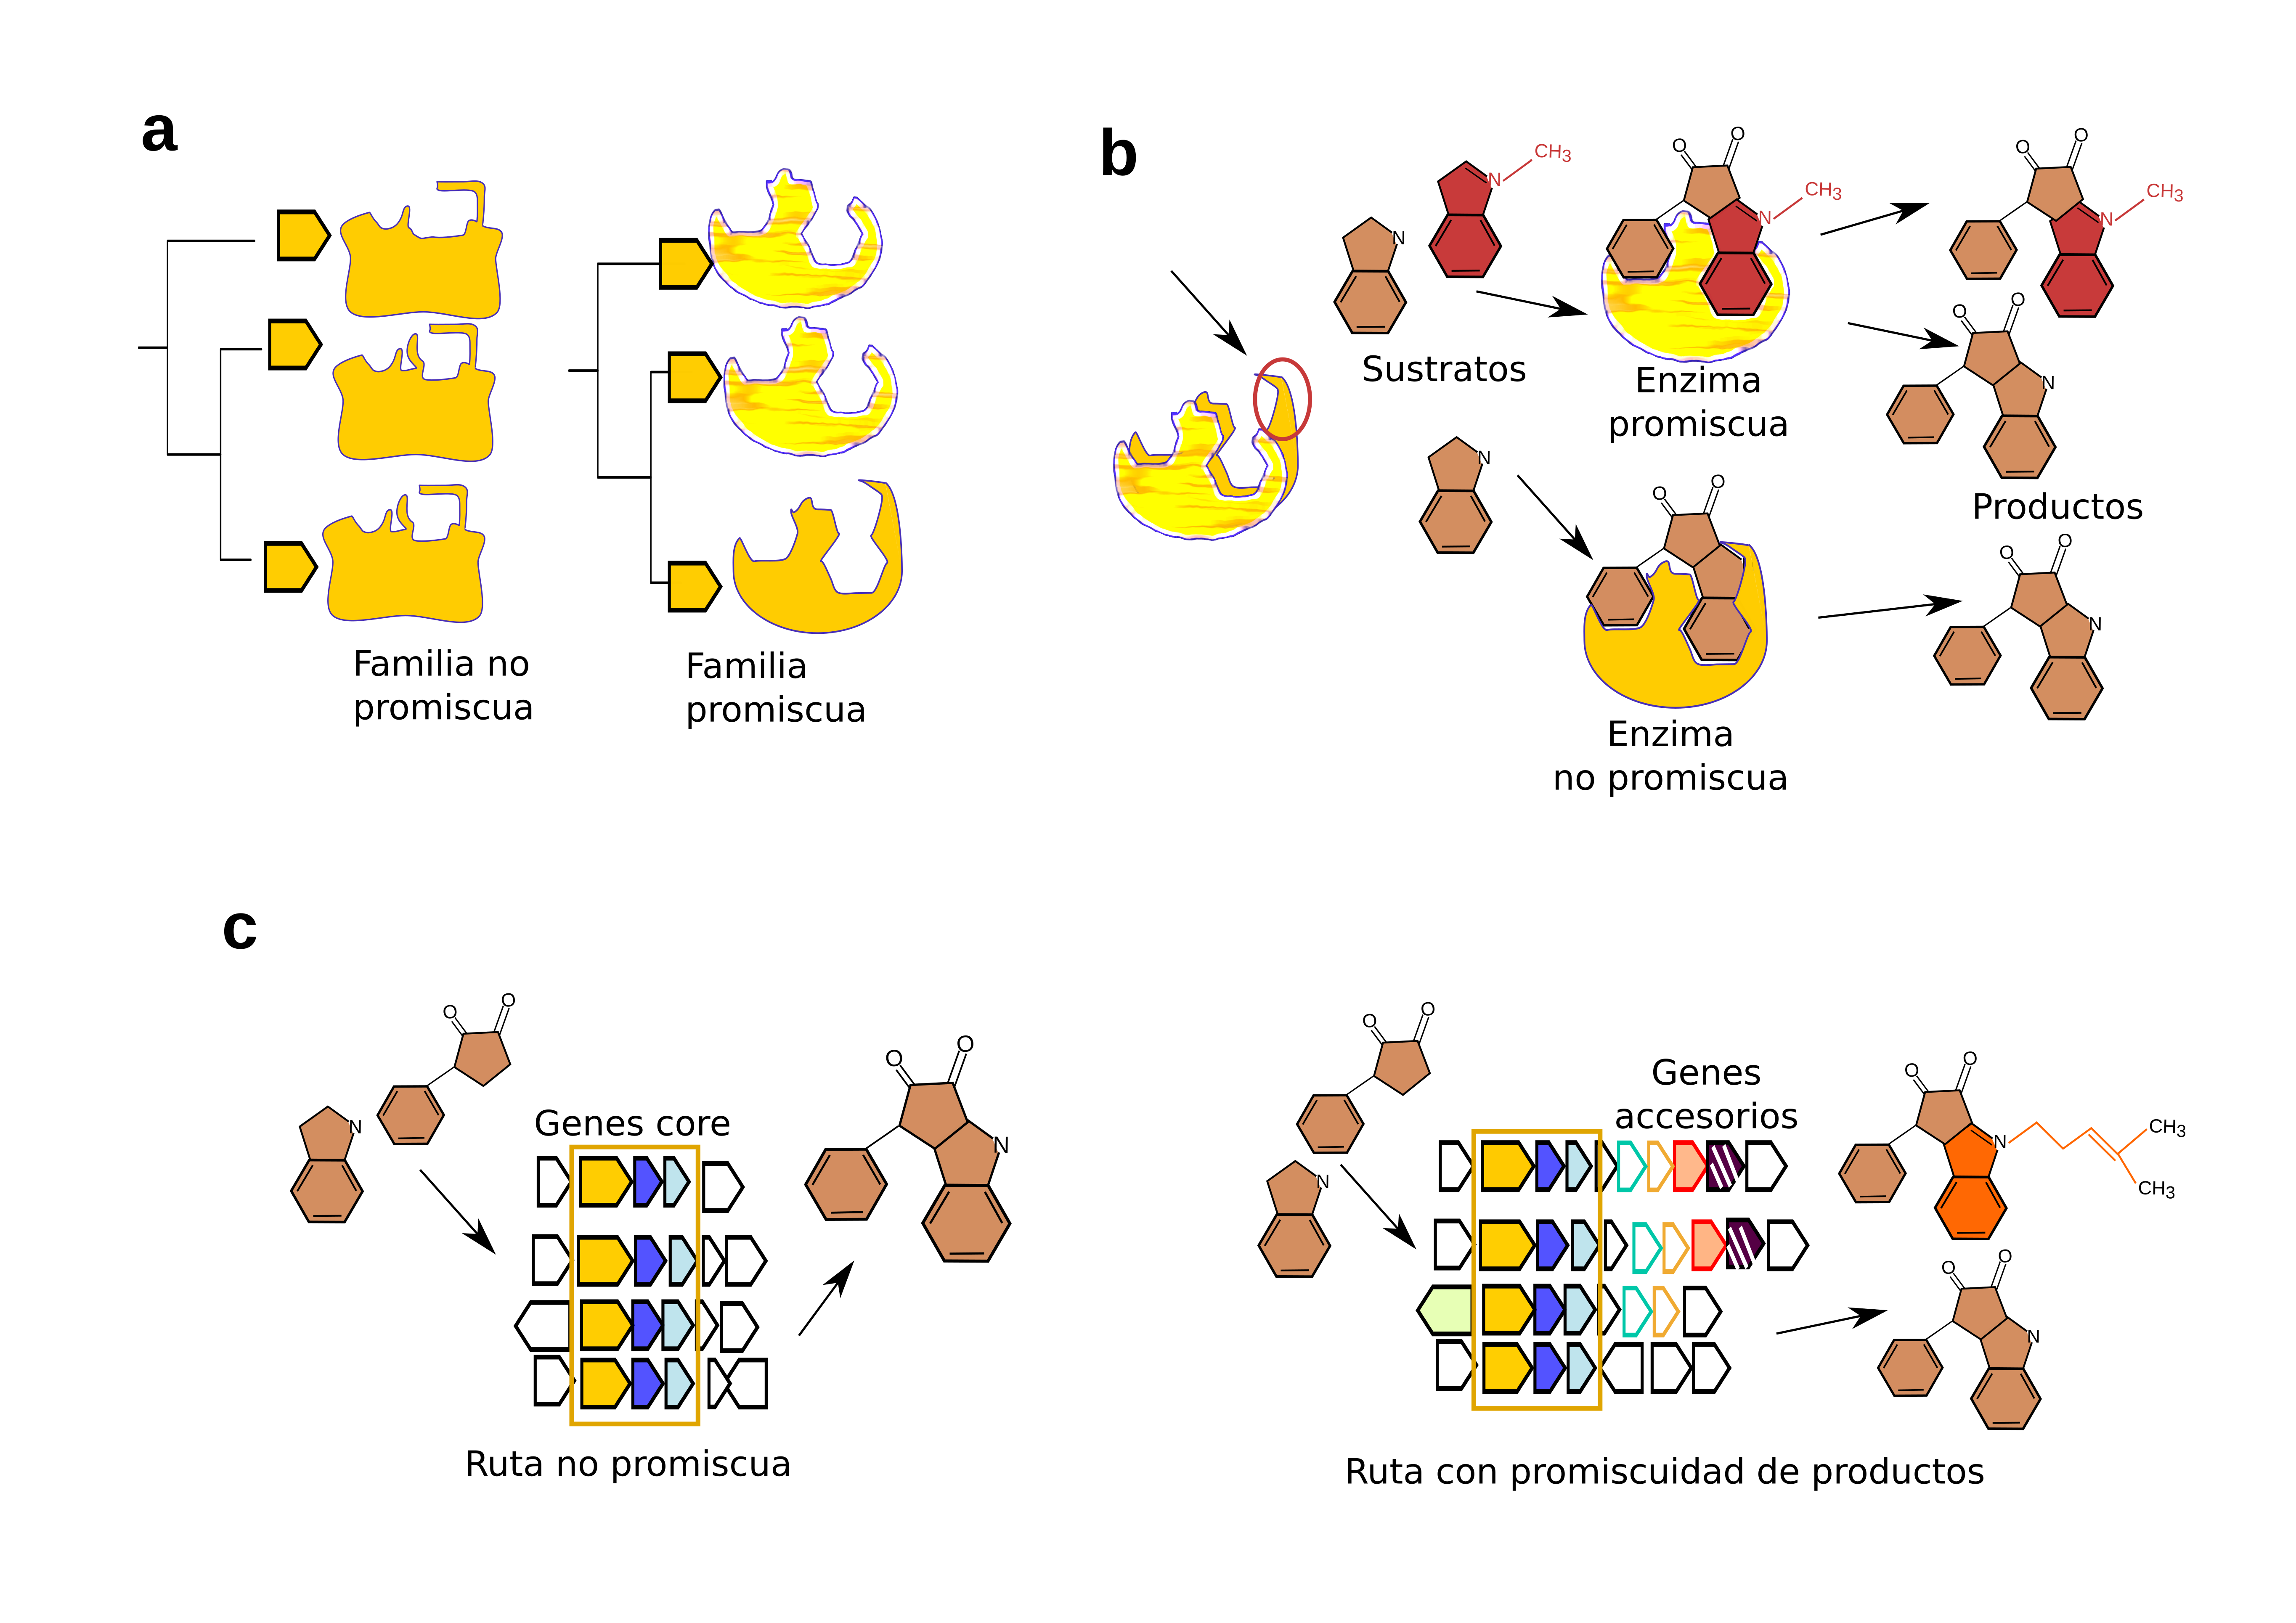
\includegraphics[angle = 0,scale = 0.6]{chapter0/NivelesPromiscuidad.png}
  \caption[Antecedentes Conceptuales]{\normalsize{Antecedentes Conceptuales}}
  \label{fig:La promiscuidad puede entenderse a distintos niveles metabólicos: enzima, familia enzimática y ruta biosintética}
  \end{figure}
  
  \nocite{}
  \nocite{@nobeli_protein_2009,@lamble_archaea_promiscuou_pathways_2003,@weng_promiscuity_specialized_pathways_2012,@baronagomez_occurrence_2003,@juarez-vazquez_evolution_2017}
  
  \section{La promiscuidad puede abordarse a distintos niveles incluyendo
  enzima, familia y ruta de
  metabólica.}\label{la-promiscuidad-puede-abordarse-a-distintos-niveles-incluyendo-enzima-familia-y-ruta-de-metabolica.}
  
  Si se entiende a la promiscuidad como funciones alternativas de alguna
  unidad molecular, puede observarse promiscuidad a distintos niveles:
  desde un mismo gen que presenta splicing alternativo, una misma enzima
  con funciones alternativas, o bien una familia enzimática donde al menos
  algunos homologos codifican enzimas promiscuas
  {[}\protect\hyperlink{ref-nobeli_protein_2009}{20}{]}. Existen también
  rutas que generan productos metabólicos
  alternativos{[}\protect\hyperlink{ref-lamble_archaea_promiscuou_pathways_2003}{68}{]},
  si se considera como la unidad de estudio a una ruta biosintética
  podemos generalizar la noción de promiscuidad al concepto de rutas
  promiscuas. La \emph{Figura 1} muestra tres niveles en los que se puede
  estudiar la promiscuidad: i) Distinguiendo familias de enzimas
  promiscuas de familias especialistas, ii) Distinguiendo enzimas
  específicas de enzimas especialistas en una familia enzimática promiscua
  y finalmente iii) encontrando promiscuidad en rutas de metabolismo
  especializado.
  
  PriA en Actinobacteria y HisA en enterobacteria son familias que ambas
  isomerizan proFAR en la ruta de síntesis de histidina pero solo la
  familia PriA es promiscua pues puede además isomerizar el sustrato PRA
  durante la síntesis de triptofano
  {[}\protect\hyperlink{ref-baronagomez_occurrence_2003}{5}{]}. Sin
  embargo dentro de Actinobacteria, existen miembros no promiscuos de
  PriA, en algunas especies de Actinomyces los homólogos de \emph{priA}
  codifican para enzimas monofuncionales en alguno de los dos sustratos,
  al menos en análisis in vitro
  {[}\protect\hyperlink{ref-juarez-vazquez_evolution_2017}{70}{]}. Así
  pues dentro de una familia promiscua no todos los miembros tienen esta
  propiedad.
  
  En este trabajo se buscará encontrar marcas de promiscuidad a nivel
  familia, enzima y ruta biosintética en el metabolismo especializado.
  
  \begin{figure}[h!tbp]
  \centering
  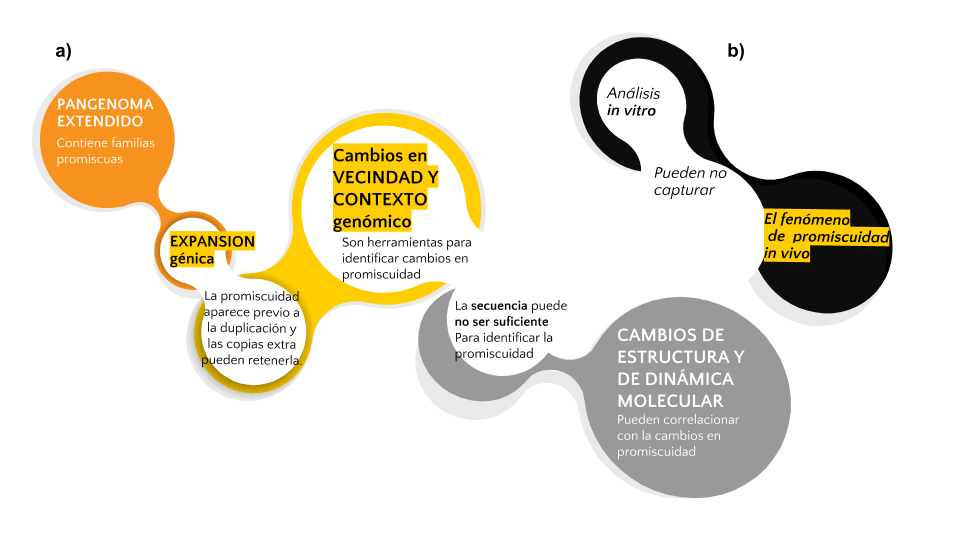
\includegraphics[angle = 0,scale = 0.5]{chapter0/AntecedentesConceptuales.png}
  \caption[Antecedentes Conceptuales]{\normalsize{Antecedentes Conceptuales}}
  \label{fig:Antecedentes conceptuales de promiscuidad}
  \end{figure}
  
  \nocite{@carbonell_molecular_2010,@juarez-vazquez_evolution_2017,@noda_tesis_2012,@soskine_mutational_2010,@aharoni_evolvability_2005,@bloom_neutral_2007,@zhao__function_prediction_neighbourhood_2014,@juarez-vazquez_evolution_2017,@martinez-nunez_lifestyle_2015,@zou_evolution_2015, @gatti-lafranconi_flexibility_2013}
  
  \section{Antecedentes conceptuales}\label{antecedentes-conceptuales}
  
  Se ha intentado identificar enzimas promiscuas mediante aprendizaje
  máquina utilizando únicamente la secuencia de aminoácidos. Estos
  enfoques no han distiguido entre identificación de familias promiscuas e
  identificación a nivel de enzima.
  {[}\protect\hyperlink{ref-carbonell_molecular_2010}{36}{]} Hasta ahora
  al utilizar únicamente la información de la secuencia no ha sido posible
  identificar una familia promiscua sin conocer previamente al menos un
  miembro promiscuo de ella. Por otra parte, diferenciar la promiscuidad a
  nivel de enzima se dificulta cuando la identidad de secuencia es alta,
  como en el caso de las PriA que han perdido la promiscuidad en
  Actinomyces
  {[}\protect\hyperlink{ref-juarez-vazquez_evolution_2017}{70}{]}
  
  Para mejorar nuestro entendimiento del fenomeno además de la comparación
  de secuencias es necesario integrar otros elementos al análisis, Figura
  2. Es difícil medir la promiscuidad en términos absolutos, por ejemplo,
  no se puede aseverar que una enzima es no promiscua sin haber
  previamente descartado todos los posibles sustratos del universo
  químico. Además incluso enzimas que resultan no promiscuas en análisis
  in vivo si son promiscuas al examinarlas in vivo
  {[}\protect\hyperlink{ref-noda_tesis_2012}{71}{]}. Sin embargo debido a
  que al adquirir una nueva función existe un umbral donde la función
  ancestral es conservada, es plausible estudiar transformar el problema
  de encontrar promiscuidad al de encontrar cambios en promiscuidad al
  relacionar estos últimos con las huellas que dejan los cambios
  funcionales{[}\protect\hyperlink{ref-soskine_mutational_2010}{33}{]}.
  Entre los elementos relevantes que correlacionan con la adquisición de
  una función alternativa se encuentran además de divergencia de
  secuencia, diversidad en vecindad
  genomica{[}\protect\hyperlink{ref-zhao__function_prediction_neighbourhood_2014}{72}{]},
  la perdida o ganancia de
  genes{[}\protect\hyperlink{ref-juarez-vazquez_evolution_2017}{70}{]},
  las expansiones genicas, i.e.~el crecimiento del pangenoma endtro de un
  grupo taxonómico
  {[}\protect\hyperlink{ref-martinez-nunez_lifestyle_2015}{26}{]} y
  finalmente cambios estructurales o de flexibilidad durante la dinámica
  molecular{[}\protect\hyperlink{ref-zou_evolution_2015}{13}{]}. Estos
  elementos tienen en común que reflejan un cambio en alguna propiedad
  genómica o biofísica observable en el registro evolutivo, de lo que se
  deriva que el buscar cambios en la promiscuidad de una enzima, familia o
  ruta, resulta mas factible por ahora que la búsqueda intrínseca de
  promiscuidad.
  
  Debido a la abundancia de datos genómicos los primeros capítulos de este
  trabajo se centran en encontrar variaciones en secuencia, distribución
  del pangenoma, y vecindades genómicas para encontrar candidatos de
  familias, enzimas y rutas promiscuas.\\
  
  \section{El establecimiento de un marco de conservación permite
  distinguir
  cambios}\label{el-establecimiento-de-un-marco-de-conservacion-permite-distinguir-cambios}
  
  La función de una enzima es un concepto jerárquico, dependiente de la
  filogenia de un organismo
  {[}\protect\hyperlink{ref-szklarczyk_string_2015}{73}{]}. Por ello, para
  poder encontrar marcas de cambio funcional, por ejemplo diferencias en
  número de copias de una familia, primero es importante trabajar en la
  construcción de un marco filogenético consistente que permita ordenar
  inclusive organismos de la misma especie. La dificultad de esta tarea
  consiste en que si los organismos que se desea ordenar son muy cercanos,
  marcadores clásicos como el 16s son también muy parecidos en secuencia y
  no permiten resolver las relaciones entre ellos. Este caso dificultó la
  construcción de un árbol filogenético de \emph{Actinomyces} y con ello
  se imposibilitaba encontrar patrones en la matriz de presencia /
  ausencia de genes
  {[}\protect\hyperlink{ref-juarez-vazquez_evolution_2017}{70}{]}.
  
  Para solventar la falta de resolución de genes individuales en
  organismos cercanos puede utilizarse el conjunto de todos los genes
  comunes en un linaje. Este conjunto es conocido como el core genome. Se
  han desarrollado herramientas bioinformáticas para este problema, por
  ejemplo phyloPhlan fija 400 genes comunes en bacteria y trata de
  localizarlos dado un conjunto de genomas sin importar su linaje
  {[}\protect\hyperlink{ref-segata_phylophlan_2013}{74}{]}. Sin embargo el
  contenido de genomas procariontes suele ser muy variable debido a
  mecanismos como transferencia horizontal y duplicación génica
  {[}\protect\hyperlink{ref-land_insights_2015}{75}{]}. Esta variabilidad
  puede dificultar encontrar muchos de estos 400 genes o bien puede ser
  que en cierto linaje no sean tan informativos. Entre organismos de la
  misma especie pueden suceder fenómenos como que el core siempre se
  reduzca al aumentar un nuevo genoma y que el conjunto total de familias
  geńicas (pangenoma) siempre aumente. Aunado a esta observación biológica
  están también las limitaciones técnicas, hay genes que no aparecen en un
  genóma porque este fue mal secuenciado o ensamblado y por lo tanto estos
  genes disminuyen el tamaño del core.
  
  Asi pues para distinguir cambios genómicos ayuda establecer primero un
  orden entre los genomas del linaje a analizar. Para ello, un camino es
  localizar los genes del core exclusivos de cada grupo de genomas y
  libres de parálogos. Aunque al momento existe publicada \emph{metaphor},
  una herramienta de selección de ortólogos
  {[}\protect\hyperlink{ref-van_der_veen_metaphor_2014}{77}{]}, al
  comenzar este trabajo no existía un método disponible para ello.
  Finalmente una vez obtenidos los genes del core es deseable contar con
  un algoritmo que además los concatene y entregue un árbol filogenético.
  
  \section{La genómica comparativa como herramienta en la distinción de
  familias y enzimas promiscuas que participan en el metabolismo
  especializado.}\label{la-genomica-comparativa-como-herramienta-en-la-distincion-de-familias-y-enzimas-promiscuas-que-participan-en-el-metabolismo-especializado.}
  
  Una parte del metabolismo especializado está compuesta por familias
  enzimáticas que evolucionaron de rutas de metabolismo central
  {[}\protect\hyperlink{ref-caetano-anolles_origin_metabolism_2009}{78}{]}.
  En las familias expandidas, ya sea por duplicación o por transferencia
  horizontal, las expansiones pueden retener la función química de las
  rutas centrales
  {[}\protect\hyperlink{ref-schniete_expanding_2018}{79}{]}, así como
  también la función alternativa suele estár presente presente aún a bajos
  niveles antes de la divergencia o duplicación
  {[}\protect\hyperlink{ref-soskine_mutational_2010}{33}{]}. Por tanto las
  familias con expansiones en un linaje son candidatas a ser familias
  promiscuas en él. Se ha notado que en el linaje en que una familia
  enzimática es promiscua hay una zona de cambio en promiscuidad
  {[}\protect\hyperlink{ref-noda-garcia_insights_2015}{39}{]}, Las
  expansiones de rutas centrales que participan en la síntesis de
  productos naturales son candidatos a presentar cambios en promiscuidad
  tanto a nivel familia como a nivel enzima.
  
  por ello la observación de la retención de función ancestral al aparecer
  una función alternativa proporciona una zona favorable para la búsqueda
  de promiscuidad a nivel de enzima. En la familia existirá un gradiente
  de promiscuidad, las más cercanas a la zona de duplicación o divergencia
  tienen más posibilidades de tener un cambio en promiscuidad que las más
  conservadas y cercanas al metabolismo central.
  
  Después de que en la sección anterior se estableció la posibilidad de
  mejorar las relaciones filogenéticas de un linaje, se abre la
  posibilidad de buscar en él expansiones de familias génicas de
  metabolismo central. Estas copias extra son candidatas a pertenecer a
  rutas de metabolismo especializado. Como prueba de concepto esta idea de
  minar genomas incorporando información evolutiva permitió la
  identificacion de la biosintesis de arsenolipidos
  {[}\protect\hyperlink{ref-cruz-morales_phylogenomic_2016}{52}{]}. La
  busqueda de productos naturales cuenta entre sus premisas que estos se
  producen en vecindades genomicas llamadas clusters y que ademas clusters
  cercanos (ya sea en contenido genico o en la secuencia de sus
  componentes), exploran variaciones metabolicas, es decir sus enzimas
  catalizan reacciones sobre sustratos parecidos aunque no identicos
  {[}\protect\hyperlink{ref-cruz-morales_phylogenomic_2016}{52}{]}.
  
  La primera versión de evomining cuenta con 200 genomas de
  Actinobacteria, una base de datos de secuencias de enzimas de productos
  naturales y otra base de datos de secuencias de enzimas de rutas
  centrales curada a mano.
  
  1 ARTS {[}\protect\hyperlink{ref-alanjary_antibiotic_2017}{80}{]} 2
  EvoMining
  {[}\protect\hyperlink{ref-cruz-morales_phylogenomic_2016}{52}{]} Se ha
  avanzado en archaea
  {[}\protect\hyperlink{ref-martinez-nunez_promiscuity_Archaea_2017}{81}{]}
  
  Desarrollarla en combinacion con algoritmos de busqueda de cambios en la
  vecindad genomica la haran una plataforma ideal para abordar el problema
  de las familias, proporcionando una solucion a la dificultad de no tener
  conocimiento previo de un miembro promiscuo en la familia investigada.
  
  Respecto al problema de los miembros, se propone explorar variaciones en
  vecindad genomica, flujo genico y dinamica molecular, como candidatos a
  reflejar la variacion en promiscuidad. Finalmente,
  
  tomando como modelo biologico el phylum Actinobacteria, un grupo de
  bacterias reconocido por su diversidad metabolica donde se ha probado la
  existencia de promiscuidad enzimatica.
  
  Evomining es una plataforma bioinformatica pensada para la
  identificacion de productos naturales\\
  Si se combinara evomining con la premisa de que vecindades distintas son
  marcadoras de funciones quimicas distintas, al encontrar una familia
  expandida con vecindades genomicas diferentes se podria solventar la
  deficiencia de otros metodos bioinformaticos consistente en que para
  identificar familias promiscuas se debe conocer previamente un miembro
  promiscuo de la misma. (Fig 4) Asi pues al combinar evomining con
  herramientas de vecindad genomica tanto de comparacion como de
  visualizacion estaremos mejorando su funcionalidad en la identificacion
  de familias promiscuas. En la siguiente sección BLA BKA
  
  la variación es la materia prima de la evolucion.
  
  \section{La genómica comparativa como herramienta en la priorización de
  clusters
  promiscuos}\label{la-genomica-comparativa-como-herramienta-en-la-priorizacion-de-clusters-promiscuos}
  
  La promiscuidad nos interesa por su produccion de variantes. Si bien en
  rutas centrales rescata la función en metaboismo secundario crea nuevas
  variantes moleculares que permiten adaptación, de hecho pangenomas
  grandes correlacioan con aparición de nuevas funciones enzimáticas.
  Considero que el concepto de promiscuidad puede ser extendido a un nuevo
  niivel. Promiscuidad enzimatica, promiscuida de familia, promiscuidad de
  cluster. En rutas centrales robustez, pero en metabolismo secundario
  platicidad. Pangenoma abierto cerrado, Aqui proponemos organizar los
  clusters y finalmente la medida de su apertura. variantes de clusters
  producen nuevos compuestos, ya sea por promiscuidad enzimática en un
  core conservado o por variación en la presencia / ausencia de genes. Un
  cluster recibe los mismos sustratos y los transforma en diferentes
  productos.
  
  \subsection{Expansion y contextos genomicos como herramienta de
  anotacion
  funcional}\label{expansion-y-contextos-genomicos-como-herramienta-de-anotacion-funcional}
  
  Al evaluar la herramienta de análisis de promiscuidad PROMISE
  {[}\protect\hyperlink{ref-carbonell_molecular_2010}{36}{]} en un set de
  datos de la familia HisA/PriA
  {[}\protect\hyperlink{ref-noda-garcia_insights_2015}{39}{]} obtuve que
  en su mejor desempeño es (huella molecular de tamaño 6) clasifica
  correctamente casi todas las no promiscuas, (HisA) pero no sucede lo
  mismo con la familia PriA donde tiene exito en 16 de 45 casos. Al
  aplicar el mismo tamaño de huella a 9 miembros promiscuos de la familia
  IlvC no consigue predecir correctamente ninguno de ellos reflejando tal
  vez que en su conjunto de entrenamiento no había miembros promiscuos
  ilvC. Por lo menos para estas familias el conjunto de entrenamiento o
  los descriptores no son suficientes para la anotacion de promiscuidad.
  
  La diversidad enzimática existente es el resultado de un proceso de
  expansion, mutacion y seleccion que se ha desarrollado durante el
  transcurso de la historia evolutiva
  {[}\protect\hyperlink{ref-khersonsky_enzyme_2010}{1}{]}. Existe
  evidencia de que cierto grado de promiscuidad o divergencia funcional
  precede a la duplicacion genica
  {[}\protect\hyperlink{ref-hughes_evolution_1994}{62}{]}. Por este motivo
  detectar expansiones ya sea duplicaciones o transferencias horizontales
  {[}\protect\hyperlink{ref-treangen_horizontal_2011}{83}{]}, puede ser un
  buen punto de partida para determinar divergencia funcional y
  promiscuidad. No todas las expansiones denotan cambio de funcion
  enzimatica, algunas pueden ser meros accidentes, sin embargo dado que la
  funcion de una enzima suele estar relacionada con sus vecinos
  {[}\protect\hyperlink{ref-overbeek_use_1999}{84}{]}, una expansion en
  una vecindad genomica diferente de la tradicional sera un referente de
  adquisicion de una nueva funcion y entonces un indicador de existencia
  previa de promiscuidad.
  
  Para sistematizar el estudio de contextos y vecindades genomicas se
  desarrollo Search Tool for the Retrieval of Interacting Genes/Proteins
  STRING {[}\protect\hyperlink{ref-snel_string_2000}{85}{]}, que cuenta
  con una anotacion de ortologia jerarquica y consistente, realizada en
  2000 organismos en cuyo marco interacciones de proteinas con
  implicaciones funcionales son predichas tanto de novo por informacion
  genomica de co-ocurrencia como por mineria de datos en articulos
  publicados. STRING es una base de datos, y como tal no permite agregar
  nuevos genomas para su analisis. Sus 2000 organismos incluyen especies
  tanto bacterianas como eucariotas. Al existir tanta diversidad, los
  genomas disponibles para un genero o clase especificos son escasos,
  p.~g. de los mas de 300 genomas disponibles de Streptomyces solo 24
  estan incluidos.
  
  Para resolver la baja cobertura de STRING hacia ciertos grupos
  taxonomicos se pueden desarrollar scripts de vecindad genomica
  utilizando RAST (Rapid Annotation using Subsystem Technology); un
  servicio interactivo de anotacion automatica de genomas de bacterias y
  arqueas {[}\protect\hyperlink{ref-aziz_rast_2008}{86}{]} donde la
  funcion de cada gen se asigna de acuerdo a conocimiento previo de
  subsecuencias de organismos cercanos filogeneticamente, cuando es
  posible se incluye en un subsistema metabolico. Estamos en una era de
  explosion de datos genomicos, proximamente se espera contar con millones
  de genomas bacterianos incluso provenientes de bacterias no cultivables,
  por ello los algoritmos deben ser constantemente optimizados a los
  nuevos volumenes de datos
  {[}\protect\hyperlink{ref-medema_computational_2015}{44}{]}. Ante esta
  expectativa seria muy util desarrollar algoritmos de analisis genomico
  que sean de codigo libre o al menos interactivos para que cada
  laboratorio pueda personalizarlos para sus propios genomas.
  
  Finalmente, no solo la vecindad genomica inmediata puede ser utilizada
  como distintivo en la busqueda de promiscuidad, diferencias en el
  contexto genomico en genes relacionados con una enzima promiscua, sin
  importar su ubicacion dentro del genoma tambien pueden ser relevantes
  para la perdida o ganancia de funcion quimica
  {[}\protect\hyperlink{ref-noda-garcia_evolution_2013}{41}{]}, (Juarez
  Vazquez et al 2015).
  
  \subsection{Contexto y vecindades
  genomicas}\label{contexto-y-vecindades-genomicas}
  
  En 2012 fueron analizados 102 genomas de 29 familias de Actinobacteria
  {[}\protect\hyperlink{ref-noda_tesis_2012}{71}{]}. sugiriendo que al
  menos en \emph{Corynebacteria} el contexto y la vecindad genomica
  incidian en la sub-funcionalizacion de PriA en subHisA
  {[}\protect\hyperlink{ref-noda-garcia_evolution_2013}{41}{]}. Respecto a
  IlvC, otra familia involucrada en la sintesis de aminoacidos fue
  estudiada y caracterizada bioquimicamente en 1 Corynebacterium y 8
  Streptomyces
  {[}\protect\hyperlink{ref-verdel-aranda_molecular_2015}{42}{]}. Para
  ampliar estos resultados, utilizando la anotacion de RAST y una
  generalizacion de la definicion de vecindad de STRING, se diseño un
  algoritmo para identificar vecindades similares asi como uno de
  visualizacion de contexto, ambos disponibles como software libre en
  github \href{https://github.com/nselem/perlas}{nselem/perlas} .
  
  El algoritmo de clasificacion de vecindades permite agruparlas en
  clusters y calificar estos clusters segun su conservacion dado un grupo
  de bacterias. La definicion de vecindad y similitud de vecindad esta
  descrita posteriormente en los metodos. El algoritmo fue aplicado a la
  familia IlvC en 290 Streptomyces resultando 9 clusters
  \href{http://148.247.230.43/nselem/CONTEXTS/REL_St275/ilvC/Contextos.php}{Datos}
  entre los mas poblados el primero cuenta con 279 elementos, otro con 9
  elemento y dos mas con 7 miembros (Fig 3), resultados experimentals son
  congruentes con que existe divergencia funcional entre miembros de
  clusters distintos
  {[}\protect\hyperlink{ref-verdel-aranda_molecular_2015}{42}{]}
  
  Natural products genomic
  era{[}\protect\hyperlink{ref-harvey_re-emergence_2015}{88}{]}
  
  \section{Estudio de una familia PriA}\label{estudio-de-una-familia-pria}
  
  \subsection{Caracterizacion in vivo}\label{caracterizacion-in-vivo}
  
  No todas las familias promiscuas provienen de expansiones, tal es el
  caso de PriA en Actinobacteria, donde no tiene expansiones y hasta el
  momento no se le conoce participación en rutas de metabolismo
  especializado.
  
  cuya promiscuidad es debida a la pérdida de TrpF Algunas enzimas PriA no
  han mostrado promiscuidad in vitro pero si in vivo ya que sobreviven en
  un medio sin triptofano, es decir in vivo complementan la funcion trpF.
  Para la construccion de cepas de Streptomyces con variantes no nativas
  de priA minimizando la modificacion genomica y el efecto de
  sobreexpresion, se planea utilizar E. coli como intermediario para
  realizar seleccion por auxotrofia. Se cuenta con un conjunto de
  plasmidos para transformar a E. coli asi como con las mutantes sencillas
  de E. coli para trpF y hisA que permiten realizar seleccion por
  auxotrofias. Ademas tenemos una coleccion de cepas nativas de
  Streptomyces asi como un mutante de PriA de S. coelicolor. Se optimizo
  una reaccion de PCR para la amplificacion de un segmento de DNA de S.
  coelicolor que contiene a priA.
  
  \subsection{Caracterizacion bioquimica in
  vitro.}\label{caracterizacion-bioquimica-in-vitro.}
  
  De la familia PriA y sus subfamilias se han caracterizado
  bioquimicamente miembros selectos de Actinomycetaceae,
  Bifidobacteriaceae, Micrococcaceae, Acidimicrobiaceae, Corynebacterium,
  Mycobacteriaceae, Streptomycetaceae, Camera (provenientes de
  metagenoma), reconstrucciones ancestrales, 80 mutantes de
  Corynebacterium, y 2 mutantes de Camera mediante cineticas enzimaticas
  para calcular las constantes Kcat,Km. El genero Streptomyces, el que
  cuenta con mayor cantidad de genomas disponibles representa una
  oportunidad muy poco explotada de explorar la influencia del contexto y
  la vecindad genomicas en secuencias de PriA (Tabla 3, Figura 5).
  
  \subsection{Modelado de dinamica
  molecular}\label{modelado-de-dinamica-molecular}
  
  La dinamica es un metodo que permite hacer simulaciones de particulas
  que sirve para obtener informacion de propiedades macroscopicas de un
  conjunto de atomos
  {[}\protect\hyperlink{ref-petrenko_molecular_2001}{89}{]}. Es util en el
  marco de mi proyecto porque permite la exploracion del espacio
  conformacional, y se ha visto que este esta relacionado con la actividad
  de la enzima {[}\protect\hyperlink{ref-sikosek_biophysics_2014}{91}{]},
  ademas dado un conformero permite verificar su estabilidad. Resuelve la
  ecuacion de movimiento de Newton con base a una configuracion inicial,
  las fuerzas interatomicas como los enlaces covalentes, las fuerzas de
  Van der Waals y la carga de las
  particulas{[}\protect\hyperlink{ref-campbell_biophysical_2012}{45}{]}.
  Entonces para generar una simulacion de dinamica molecular, debe
  contarse con una estructura como punto de partida, ya sea esta
  cristalografica o modelada de novo o por homologia. El laboratorio de
  bioinformatica y biofisica computacional ha desarrollado un protocolo de
  generacion de modelos homologos estructurales y dinamicas moleculares
  (Carrillo-Tripp et al 2015 in prep); con este pipeline se han generado
  dos estructuras de Camera
  {[}\protect\hyperlink{ref-noda-garcia_insights_2015}{39}{]}, 30
  estructuras y dinamicas de miembros de Actinobacteriaceae y
  Bifidobacteriaceae (Vazquez-Juarez et al in prep.) y finalmente una
  estructura de subHisA de Corynebacterium diphteriae. En la familia
  Streptomyces, interesante debido a su variacion en contexto genomico y
  en mediciones in vitro aun no se modelan dinamicas moleculares aunque 40
  estructuras por homologia estan en proceso.
  
  En un estudio de subHisA
  {[}\protect\hyperlink{ref-noda_tesis_2012}{71}{]} se utilizo el método
  de dinámica molecular y se comparó el número de confórmeros entre
  miembros de subHisA y PriA, resultando mayor el de PriA como corresponde
  a una enzima promiscua. El estudio sobre la relación
  dinámica-flexibilidad de \(\noindent\beta\)-lactamasas utiliza replica
  exchange, una variacion de dinamica molecular que corre replicas en
  paralelo a distintas temperaturas
  {[}\protect\hyperlink{ref-bai_replica_2006}{92}{]}. Una desventaja de
  este metodo es que por el costo computacional de las replicas agregar
  explicitamente otras moleculas a la simulacion como el solvente no es
  posible en tiempo razonable. Una vez generadas las dinamicas moleculares
  se procedera a calcular tanto el numero de conformeros como el indice de
  flexibilidad dsi {[}\protect\hyperlink{ref-zou_evolution_2015}{13}{]}.
  Se esta desarrollando PEDB, promiscuous enzyme database, una base datos
  genomicos, evolutivos, bioquimicos y estructurales y de metabolismo de
  PriA en Actinobacteria donde se procedera al analisis de los mismos
  (\url{http://148.247.230.43/nselem/PHP/queries.html}).
  
  En conclusion la promiscuidad enzimatica es un fenomeno complejo debido
  a multiples causas. Existe una gran variedad de estudios con enfoques
  puntuales sobre aspectos estructurales, dinamicos y evolutivos sin
  embargo hasta ahora no se han reportado trabajos multidisciplinarios que
  involucren a todas las partes involucradas
  
  \clearpage  
  
  \chapter*{Pregunta biológica}\label{pregunta-biologica}
  \addcontentsline{toc}{chapter}{Pregunta biológica}
  
  \clearpage  
  
  \chapter*{Objetivos}\label{objetivos}
  \addcontentsline{toc}{chapter}{Objetivos}
  
  \section{Objetivo General}\label{objetivo-general}
  
  Estudiar el fenomeno de promiscuidad enzimatica tanto desarrollando
  estrategias para identificar familias promiscuas dentro de un grupo
  taxonomico, como comparando variaciones de promiscuidad in vitro e in
  vivo con variaciones en contexto genomico y flexibilidad en miembros de
  una familia. (Figura 7)
  
  \section{Objetivos particulares}\label{objetivos-particulares}
  
  Mejorar evomining como metodo de identificacion de familias enzimaticas
  promiscuas aprovechando los cambios en vecindades genomicas como
  caracteristicas informativas provenientes de datos filogenomicos.
  Estudiar la relacion entre historias filogenomicas y procesos biofisicos
  con la promiscuidad in vitro, a traves de mediciones de ciertas
  caracteristicas de la familia PriA. Caracterizar cambios de promiscuidad
  enzimatica in vivo mediante perfiles metabolomicos de actividades de
  PriA y enzimas asociadas.
  
  \clearpage  
  
  \chapter*{Estrategias}\label{estrategias}
  \addcontentsline{toc}{chapter}{Estrategias}
  
  \subsubsection{Obtener informacion genomica del phylum
  Actinobacteria.}\label{obtener-informacion-genomica-del-phylum-actinobacteria.}
  
  Colectar genomas de Actinobacteria de NCBI y de colecciones privadas.
  
  \subsection{Anotar consistentemente las secuencias codificantes de estos
  genomas.}\label{anotar-consistentemente-las-secuencias-codificantes-de-estos-genomas.}
  
  Utilizar un anotador automatizado y desarrollar los scripts necesarios
  para anotar los genomas.
  
  \subsubsection{Establecer las relaciones filogeneticas de los genomas
  colectados.}\label{establecer-las-relaciones-filogeneticas-de-los-genomas-colectados.}
  
  Mediante el uso del core genome construir un arbol filogenomico que
  permita establecer un marco sobre el cual hablar de cambio y que
  facilite reclasificar los genomas mal nombrados.
  
  \subsection{La promiscuidad en familias
  enzimaticas.}\label{la-promiscuidad-en-familias-enzimaticas.}
  
  Mejorar Evomining mediante la identificacion de cambios de vecindad
  genomica en familias selectas de metabolismo central convirtiendola en
  una plataforma de codigo libre disponible para otros investigadores.
  
  \paragraph{Identificar cambios en la vecindad genomica en familias
  selectas de enzimas de metabolismo
  central.}\label{identificar-cambios-en-la-vecindad-genomica-en-familias-selectas-de-enzimas-de-metabolismo-central.}
  
  Clasificar sistematicamente las secuencias de familias codificantes
  segun su similitud en familias enzimaticas.\\
  Desarrollar las herramientas bioinformaticas necesarias para separar
  clusters de vecindades genomicas.
  
  \subsubsection{Promiscuidad in vitro dentro de miembros de una familia
  promiscua de
  enzimas.}\label{promiscuidad-in-vitro-dentro-de-miembros-de-una-familia-promiscua-de-enzimas.}
  
  Dados los sustratos conocidos de PriA investigar las posibles
  correlaciones entre mediciones de constantes cataliticas, contexto
  genomico, vecindad genomica, numero de conformeros e indice de
  flexibilidad.
  
  \subsubsection{Sistematizar Evomining para convertirla una plataforma
  descargable y utilizable en cualquier set de datos bacterianos
  relacionados taxonomicamente proporcionados por el
  usuario.}\label{sistematizar-evomining-para-convertirla-una-plataforma-descargable-y-utilizable-en-cualquier-set-de-datos-bacterianos-relacionados-taxonomicamente-proporcionados-por-el-usuario.}
  
  Ampliar el contenido de Evomining al integrar los genomas colectados de
  Actinobacteria. Sistematizar la base de datos de metabolismo central.\\
  Desarrollar la visualizacion e integrar la clasificacion de vecindades
  genomicas como una herramienta adicional en la busqueda de promiscuidad.
  
  \subsubsection{Seleccionar miembros homologos de la familia de
  enzimas.}\label{seleccionar-miembros-homologos-de-la-familia-de-enzimas.}
  
  Se escogieron 41 Streptomyces repartidos en un arbol de rpoB de 400
  Streptomyces con genoma disponible. Esta seleccion incluye los seis
  Streptomyces de los que se cuenta con cinetica enzimatica de PriA, tres
  de ellos con estructura cristalografica.
  
  \subsubsection{Medir cineticas enzimaticas, contexto genomico, vecindad
  genomica, flexibilidad y numero de
  conformeros.}\label{medir-cineticas-enzimaticas-contexto-genomico-vecindad-genomica-flexibilidad-y-numero-de-conformeros.}
  
  Determinar la pertenencia a uno de cuatro posibles contextos genomicos
  respecto al gen trpF. Estudiar la existencia de distintas vecindades
  genomicas. Determinar la cinetica enzimatica de 9 enzimas mas buscando
  variabilidad en contexto genomico (sugeridas en la tabla 4). Obtener
  mediante una colaboracion 37 modelos estructurales por homologia y
  modelar dinamica molecular.
  
  La siguiente tabla contiene la diversidad de contextos y vecindades
  genomicas de 41 Streptomyces respecto al gen trpF.
  
  \subsubsection{Determinar posibles correlaciones entre los datos
  producidos.}\label{determinar-posibles-correlaciones-entre-los-datos-producidos.}
  
  Numero de conformeros e indice de promiscuidad.\\
  indice de flexibilidad y numero de conformeros.\\
  Numero de conformeros y contexto genomico.\\
  indice de flexibilidad y contexto genomico.\\
  Contexto genomico e indice de promiscuidad I.\\
  Analizar las vecindades genomicas e indice de promiscuidad I.
  
  \subsection{Desarrollar una metodologia para la deteccion in vivo de
  promiscuidad
  enzimatica.}\label{desarrollar-una-metodologia-para-la-deteccion-in-vivo-de-promiscuidad-enzimatica.}
  
  Debido a cambios en flexibilidad o cambios de contexto genomico, se
  puede sospechar de diferencias en la funcion quimica de dos miembros de
  una familia de enzimas, sin conocer las diferencias a nivel de
  sustratos. Para investigar estos cambio in vivo se propone estudiar
  diferencias en perfiles metabolomicos de una coleccion de cepas en
  condiciones diversas.
  
  \clearpage  
  
  \chapter*{Metodologia}\label{metodologia}
  \addcontentsline{toc}{chapter}{Metodologia}
  
  A continuacion describiré la metodologia para cada una de las
  estrategias expuestas previamente. Todos los scripts desarrollados
  fueron escritos en perl y estan disponibles en github
  \url{https://github.com/nselem/perlas}.
  
  \subsection{La promiscuidad en familias
  enzimaticas.}\label{la-promiscuidad-en-familias-enzimaticas.-1}
  
  \subsubsection{Actinobacteria genomica}\label{actinobacteria-genomica}
  
  Para obtener informacion genomica del phylum Actinobacteria mediante la
  coleccion de genomas de NCBI se revisaron todas las familias de
  Actinobacteria de la base genoma de NCBI y se seleccionaron los genomas
  con minimo 5 genes por contig. Se crearon scripts para utilizar la
  interfaz e-utils de NCBI y descargar estos genomas desde la terminal a
  partir de una lista de identificadores.
  
  \subsubsection{Annotation}\label{annotation}
  
  Para anotar consistentemente las secuencias codificantes de estos
  genomas se utilizo el anotador automatizado RAST y se desarrollaron los
  scripts necesarios para anotar los genomas desde la terminal, conectado
  asi NCBI y RAST.
  
  \subsubsection{Genomic DB phylogeny}\label{genomic-db-phylogeny}
  
  Establecer las relaciones filogeneticas de los genomas colectados.
  Mediante el uso del core genome para construir un arbol filogenomico,
  para reclasificar los genomas mal nombrados.\\
  Para obtener el core genome y en base a el reclasificar los genomas se
  diseño el algoritmo estrellas basado en Best Bidirectional Hits (blast
  all vs all).
  
  Estrellas. Se realiza un blast all vs all de genomas deseados. Para cada
  secuencia, centrado en cada genoma se realiza una lista (estrella) de
  sus mejores hits bidireccionales. Si las listas de todos los genomas
  coinciden es un BBH multiple y se agrega la lista al core genome. (Fig
  9) Una vez con el core genome completo se puede reconstruir la
  filogenia. Este metodo fue exitoso en la deteccion de una familia
  marcadora de Clavibacter michiganensis (2014 Rodriguez-Orduña in prep).
  
  \subsection{Identificar cambios en la vecindad genomica en familias
  selectas de enzimas de metabolismo
  central.}\label{identificar-cambios-en-la-vecindad-genomica-en-familias-selectas-de-enzimas-de-metabolismo-central.-1}
  
  Clasificar sistematicamente las secuencias de familias codificantes
  segun su similitud en familias enzimaticas.
  
  Como se menciono en los antecedentes, se han separado 888 genomas de
  Actinobacteria en 3 grupos taxonomicos utilizando para la anotacion la
  tecnologia de subsistemas de RAST. Para la separacion en familias iso
  funcionales (ortologos, paralogos y expansiones) n se utilizo RAST,
  especificamente el script What Changed (WC) que asigna un numero a cada
  familia, esta herramienta esta basada en k-mers, su codigo esta
  disponible en github:
  (\url{https://github.com/kbase/kbseed/blob/master/service-scripts/svr_CS.pl}).
  Ademas de en los tres grupos ya mencionados, tambien se realizara una
  clasificacion para trescientos genomas de Actinobacteria distribuidos en
  todas sus familias taxonomicas.
  
  Para desarrollar las herramientas bioinformaticas necesarias para
  separar clusters de vecindades genomicas a continuacion se describe
  detalladamente como se definicio vecindad genomica y la relacion
  implementada de similitud.
  
  \begin{enumerate}
  \def\labelenumi{\arabic{enumi}.}
  \item
    Un conjunto expandido es un conjunto que contiene secuencias homologas
    asi como sus expansiones: paralogos y transferencias horizontales.
    Dado un conjunto de genomas, se pueden calcular y enumerar todos sus
    contextos extendidos utilizando WC.
  \item
    Un PEG es un elemento de un conjunto expandido. Dado un PEG p, se
    define CE(p) el numero del conjunto expandido de p, como el numero
    asignado por WC al conjunto expandido a que p pertenece.
  \item
    La vecindad de un PEG es el conjunto de PEGs cercanos a el. Dado un
    umbral en terminos de distancia de pares de bases entre puntos medios
    para precisar la definicion de cercano, se pueden calcular todos los
    contextos de un genoma.
  \item
    Una vecindad Aes n-similar a otra vecindad B si C=\{aA \textbar{} b B
    ,CE(b)=CE(a)\} tiene al menos cardinalidad n. Es decir si existen al
    menos n elementos de A que pertenecen al mismo conjunto expandido que
    algun elemento de B.
  \item
    Un conjunto de vecindades es un conjunto de PEGs clusterizado segun la
    relacion n-similaridad. Si A es n-similar a B y B esn-similar a C
    entonces, aun si A no fuese n-similar a C, los PEGs generadores de
    A,B,C son agrupados dentro del mismoconjunto de vecindades.
  \item
    Un cluster es un conjunto de conjunto de vecindades.
  \item
    Los clusters son evaluados segun el numero y la cardinalidad de sus
    conjuntos de vecindades.
  \end{enumerate}
  
  Sea Cl un cluster, donde CCi es un conjunto de contextos y ni es la
  cardinalidad de CCi Cl=\{CC1,CC2,\ldots{},CCk\}
  
  Sean M la cardinalidad maxima de un conjunto de contextos y m la
  cardinalidad maxima sin considerar M.
  
  \begin{Shaded}
  \begin{Highlighting}[]
  \CommentTok{#$$   M\textbackslash{}eq\textbackslash{}max_\{ni\} i\textbackslash{}eq\{1,2,..,k\}         m\textbackslash{}eq\textbackslash{}max_ni i\textbackslash{}eq \{1,2,...,k\}  ni\textbackslash{}ne\{M\}  $$}
  \end{Highlighting}
  \end{Shaded}
  
  \[\sum_{j=1}^n (\delta\theta_j)^2 \leq {{\beta_i^2}\over{\delta_i^2 + \rho_i^2}}
  \left[ 2\rho_i^2 + {\delta_i^2\beta_i^2\over{\delta_i^2 + \rho_i^2}} \right] \equiv \omega_i^2\]
  
  M representa el contexto mas difundido de la enzima, dentro del grupo
  taxonomico considerado; mes relevante porque si m es grande significa
  que hay un segundo contexto genomico conservado en dicho grupo
  taxonomico, y entonces posiblemente una ganancia de funcion.
  
  La evaluacion de Cl esta dada por una combinacion lineal de k,m y M\\
  S(Cl)=f(k,m,M)=c1k+c2m+c3M
  
  Este algoritmo se puede mejorar considerando la orientacion de los genes
  del cluster asi como clusters de los vecinos.
  
  \subsubsection{Organizar y presentar los datos en una
  plataforma.}\label{organizar-y-presentar-los-datos-en-una-plataforma.}
  
  Para contribuir al desarrollo de la plataforma Evomining se
  desarrollaran scripts de visualizacion de arboles filogeneticos y
  contextos genomicos.
  
  Para facilitar el analisis visual de una vecindad genomica ya la vez
  generar imagenes de alta calidad facilmente exportables para su uso en
  publicaciones, se desarrollaran scripts de visualizacion que utilizaran
  el formato Scalable Vector Graphics (SVG), dicho formato es basicamente
  un archivo de texto XML que contiene instrucciones para que el navegador
  realice un dibujo (W3school/SVG 2015). Al ser vectores, las imagenes
  generadas en SVG no pierden resolucion al ser escaladas y justamente por
  ser escalables permiten explorar con detalle grandes cantidades de datos
  organizados por ejemplo en arboles filogeneticos. Los scripts a
  desarrollar extraeran para cada gen informacion necesaria como
  coordenadas, direccion, funcion quimica, etc, proveniente de la
  anotacion de RAST y de los scripts de comparacion de vecindades
  genomicas. La primera version de evomining fue desarrollada en el
  lenguaje perl; este lenguaje cuenta con un modulo para facilitar la
  elaboracion de SVG (perlmaven/SVG 2015) por lo que al utilizar SVG no se
  agregan nuevos requerimientos a su desarrollo y se facilita su
  portabilidad.
  
  Se amplificara Evomining de los 200 genomas con que contaba su version
  inicial a los 880 colectados mudando la curacion manual de su base de
  datos de rutas centrales a la anotacion por subsistemas de RAST.
  Finalmente se presentara la variacion en vecindades genomicos como una
  herramienta adicional que ayude en la busqueda de promiscuidad en
  familias de enzimas pertenecientes al metabolismo central.
  
  \subsection{Promiscuidad in vitro}\label{promiscuidad-in-vitro}
  
  \subsubsection{Datos cineticos:}\label{datos-cineticos}
  
  En todos los ensayos enzimaticos se busca medir una señal que permita
  una distincion clara entre sustrato y producto
  {[}\protect\hyperlink{ref-bisswanger_general_2011}{93}{]}. La cinetica
  enzimatica de PriA proveniente del genero Streptomyces sera determinada
  como ya se ha reportado previamente, mediante el monitoreo de cambios en
  fluorescencia (isomerizacion del sustrato PRA) o en absorbancia
  (isomerizacion del sustrato PROFAR). En el caso de la isomerizacion de
  PRA, debido a que contiene un anillo de antranilato, la fluorescencia
  del sustrato PRA es 50 veces mayor que la del producto
  1-(2-carboxyphenylamino)-1-deoxy-D-ribulose 5-phosphate (CdRP) por lo
  que se utiliza la disminucion en fluorescencia como medida de la
  conversion del sustrato en producto
  {[}\protect\hyperlink{ref-hommel_phosphoribosyl_1995}{94}{]}. Se
  mandaran sintetizar estas variantes para posteriormente sobre
  expresarlas en E. coli. Se creceran cepas modificadas de E. coli (W-,
  H-) en medio minimo M9 enriquecido con una mezcla de aminoacidos excepto
  L-histidina y L-triptofano y se seleccionaran por rescate de auxotrofia.
  Para obtener la enzima necesaria para los ensayos enzimaticos se
  utilizaran plasmidos disponibles para construcciones de sobreexpresion
  de proteina, despues de la produccion la enzima se purificara utilizando
  cromatografia por afinidad a niquel
  {[}\protect\hyperlink{ref-verduzco-castro_co-occurrence_2016}{67}{]}.
  
  Finalmente se recopilaran datos cineticos de PriA tanto privados como
  los publicos reportados a la fecha en la BRaunschweig ENzyme DAtabase
  BRENDA {[}\protect\hyperlink{ref-scheer_brenda_2011}{95}{]}. Una vez
  colectados los datos se anotaran en PEDB, nuestra base de datos ad hoc,
  y se tomara como medida de promiscuidad el I-index
  {[}\protect\hyperlink{ref-nath_quantitative_2008}{12}{]} que se define
  como: I=1ln Ni=1Npi( pi) donde pi=Kicat Kim / i=1NKicatKim
  
  \subsubsection{Dinamica molecular}\label{dinamica-molecular}
  
  Para generar dinamicas moleculares primer lugar se recolectaran las
  estructuras tridimensionales de miembros de PriA de Actinobacteria.
  Despues se procedera a modelar por homologia las estructuras
  tridimensionales faltantes utilizando el pipeline del laboratorio de
  bioinformatica y biofisica computacional. Este pipeline utiliza el
  software Rosetta para el modelado para las estructuras y GROMACS
  Groningen Machine for Chemical Simulation,
  {[}\protect\hyperlink{ref-van_der_spoel_gromacs_2005}{96}{]} para el
  modelado de la dinamica molecular. Esta parte del trabajo se realizara
  en colaboracion con el laboratorio de bioinformatica y biofisica
  computacional.
  
  \subsection{Promiscuidad in vivo}\label{promiscuidad-in-vivo}
  
  Se realizaran construcciones con variantes no nativas de priA y/o trpF
  en Streptomyces coelicolor. Para las construcciones se amplificara
  mediante PCR un fragmento alrededor de PriA que se insertara en un
  vector. Este vector recombinara en E. coli con un casete provisto de un
  gen marcador de resistencia a antibiotico y este gen recombinado se
  pasara por conjugacion a S. coelicolor donde se espera que realice una
  doble recombinacion. El paso por E. coli es llevado a cabo porque
  Streptomyces no se puede transformar por electroporacion. Se
  seleccionaran las cepas de Streptomyces resistentes al antibiotico como
  prueba de que ya no poseen su priA nativa. Posteriormente, mediante un
  procedimiento analogo se sustituira el gen marcador, por variantes no
  nativas de priA/trpF.
  
  La cromatografia se refiere a un conjunto de metodos que separan y
  analizan mezclas de moleculas. Basicamente estos metodos se basan en
  diferencias en el tamaño, intercambio de iones y afinidad.
  {[}\protect\hyperlink{ref-campbell_biophysical_2012}{45}{]}
  Posteriormente se combinan con espectrometria de masas que es una
  tecnica que mide el radio masa-carga de las particulas fragmentadas en
  iones. {[}\protect\hyperlink{ref-campbell_biophysical_2012}{45}{]}. Los
  datos obtenidos de espectrometria de masas se procesaran utilizando
  redes moleculares, que consiste en agrupar los productos segun la
  similitud de sus partes. Plan: 3 replicas tecnicas, 2 replicas
  biologicas de 5 cepas.
  
  \subsection{Consideraciones}\label{consideraciones}
  
  Falsos negativos respecto a promiscuidad estan muy extendidos en la
  literatura y en las bases de datos, en parte porque la mayoria de las
  funciones son asignadas por similitud de secuencia y dado un falso
  negativo el error se propaga en secuencias similares. Por otro lado es
  muy dificil demostrar un verdadero negativo a menos que se prueben todas
  las posibilidades de sustrato para la enzima. Sin embargo el espacio de
  sustratos puede acotarse gracias a tecnicas como el docking que esta
  intimamente relacionado con la dinamica molecular
  {[}\protect\hyperlink{ref-campbell_biophysical_2012}{45}{]}. Limitar el
  espacio de sustratos puede retroalimentarse con el estudio de la
  promiscuidad in vivo y viceversa.
  
  Con los metodos propuestos en este trabajo solo se podra detectar
  perdida o ganancia de promiscuidad entre enzimas de organismos respecto
  a otros miembros dentro un grupo taxonomico, no asi el estado de
  promiscuidad intrinseco a la enzima. Si dada una enzima no se detectan
  variaciones en contexto, vecindad genomica o flexibilidad dentro de un
  grupo taxonomico cercano, entonces no podemos decir en principio nada
  acerca de la promiscuidad de la variante, posiblemente es promiscua pero
  al mantenerse constante en todos los parametros descritos, con estos
  metodos no se puede sugerir promiscuidad. Es posible que al mirar en un
  grupo taxonomico mas amplio se detecte una neofuncionalizacion de la
  familia aunque tambien es posible que exista una variable z como la
  flexibilidad de sustrato
  {[}\protect\hyperlink{ref-nobeli_protein_2009}{20}{]} que no se este
  considerando y que explique o sea el mejor indicador para esta familia
  de promiscuidad enzimatica.
  
  Se debe considerar que si existe una correlacion vecindad
  genomica-promiscuidad, esta no indica causa efecto, mas bien, es
  plausible que la vecindad sea un amplificacion de diferencias en
  secuencia, a un numero igual de variaciones en secuencia la existencia
  de un cambio de vecindad indica un proceso mas largo y mas cambios, es
  una amplificacion de las marcas dejadas por transformaciones
  funcionales.
  
  Si bien no se resuelve el problema de anotar promiscuidad
  automaticamente, este trabajo pretende aprovechar que los contextos
  genomicos ayudan a la identificacion de familias promiscuas para mejorar
  una plataforma de productos naturales, pretende tambien una confirmacion
  de que los cambios en la dinamica molecular ayudan a identificar los
  miembros mas promiscuos hacia actividades recien adquiridas, asi como
  tambien ser pionero en la investigacion de promiscuidad in vivo.
  
  Gene cluster plants{[}\protect\hyperlink{ref-osbourn_gene_2010}{98}{]}\\
  Archaeal core
  {[}\protect\hyperlink{ref-makarova_comparative_1999}{99}{]}\\
  Methanosarcina reconstruction
  {[}\protect\hyperlink{ref-benedict_genome-scale_2012}{100}{]}\\
  Archaea phylum{[}\protect\hyperlink{ref-seitz_genomic_2016}{101}{]}\\
  Prediction for possible products of promiscuous
  enzymes{[}\protect\hyperlink{ref-jeffryes_mines_2015}{102}{]}\\
  Saxitoxin {[}\protect\hyperlink{ref-moustafa_origin_2009}{103}{]}\\
  Plants clusters
  {[}\protect\hyperlink{ref-medema_computational_2016}{104}{]}\\
  MiBIG {[}\protect\hyperlink{ref-medema_minimum_2015}{105}{]}\\
  Metagenomics on Streptomyces
  {[}\protect\hyperlink{ref-iqbal_natural_2016}{106}{]}\\
  Sulfolobus reconsruction
  {[}\protect\hyperlink{ref-ulas_genome-scale_2012}{107}{]}\\
  Archaeal Natural
  products{[}\protect\hyperlink{ref-charlesworth_untapped_2015}{108}{]}\\
  Computational Pangenomics
  {[}\protect\hyperlink{ref-computational_pan-genomics_consortium_computational_2016}{109}{]}\\
  Cuántos genes ``obtenidos por EvoMining'' son core/ cloud/stand alone\\
  Qué porcentaje de genes únicos recupera EvoMining\\
  Eucarya paralogs reshape gene clusters
  {[}\protect\hyperlink{ref-chan_remodelling_2015}{110}{]}\\
  Microbial dark mater
  {[}\protect\hyperlink{ref-rinke_insights_2013}{111}{]}\\
  Archaea anaerobica carbon
  {[}\protect\hyperlink{ref-castelle_genomic_2015}{112}{]} Archaea Eucarya
  gap loki{[}\protect\hyperlink{ref-spang_complex_2015}{113}{]}\\
  Archaea and
  eucarya{[}\protect\hyperlink{ref-koonin_archaeal_2015}{114}{]}\\
  BPGA {[}\protect\hyperlink{ref-chaudhari_bpga-_2016}{115}{]} genes
  esenciales bacteria
  minima{[}\protect\hyperlink{ref-glass_essential_2006}{116}{]}\\
  Radical {[}\protect\hyperlink{ref-narechania_random_2012}{117}{]}\\
  RaxML large philogenies
  {[}\protect\hyperlink{ref-stamatakis_raxml_2014}{118}{]}\\
  R phylogenies
  {[}\protect\hyperlink{ref-phyloseq_powerful_2016}{119}{]}\\
  Streptomyces exploradores
  {[}\protect\hyperlink{ref-zacharia_exploring_2017}{120}{]}\\
  LUCA {[}\protect\hyperlink{ref-woese_universal_1998}{121}{]} Luchando
  por el reconocimiento de
  Archaea{[}\protect\hyperlink{ref-woese_are_1981}{122}{]},{[}\protect\hyperlink{ref-woese_towards_1990}{123}{]}
  The primary kingdoms
  {[}\protect\hyperlink{ref-woese_phylogenetic_1977}{124}{]}\\
  Predicccion aRchaeas
  {[}\protect\hyperlink{ref-woese_there_1994}{125}{]}\\
  RASt archaea {[}\protect\hyperlink{ref-graham_archaeal_2000}{126}{]}
  Book Archaea
  {[}\protect\hyperlink{ref-howland_surprising_2000}{127}{]}\\
  Computational methods for bacterial and archaeal genomes
  {[}\protect\hyperlink{ref-xu_computational_2008}{128}{]}\\
  Archaeas boook {[}\protect\hyperlink{ref-garrett_archaea_2008}{129}{]}\\
  GC content plasmido genoma
  {[}\protect\hyperlink{ref-nishida_evolution_2012}{130}{]} Genoma
  minimo{[}\protect\hyperlink{ref-coyle_mysteries_2016}{131}{]}\\
  Phylogeny R {[}\protect\hyperlink{ref-omeara_cran_2016}{132}{]}\\
  Cyanobacteria fluctuacion genomica y adaptacion
  {[}\protect\hyperlink{ref-larsson_genome_2011}{133}{]}\\
  Ecology of cyanobacterua
  {[}\protect\hyperlink{ref-whitton_ecology_2012}{134}{]}\\
  Histdine
  biosynthesis{[}\protect\hyperlink{ref-cohen_biosynthesis_2004}{135}{]}\\
  PriA reconstruction
  {[}\protect\hyperlink{ref-plach_long-term_2016}{136}{]}\\
  Escala temporl bacterias
  {[}\protect\hyperlink{ref-battistuzzi_genomic_2004}{137}{]}\\
  Pangenome size
  {[}\protect\hyperlink{ref-lapierre_estimating_2009}{138}{]}\\
  variabilidad del 16s
  {[}\protect\hyperlink{ref-vetrovsky_variability_2013}{139}{]}
  
  \chapter{Desarrollo de Orthocore e implementación de otras herramientas
  computacionales para entender el pangenoma de un linaje
  genómico.}\label{desarrollo-de-orthocore-e-implementacion-de-otras-herramientas-computacionales-para-entender-el-pangenoma-de-un-linaje-genomico.}
  
  \begin{figure}[h!tbp]
  \centering
  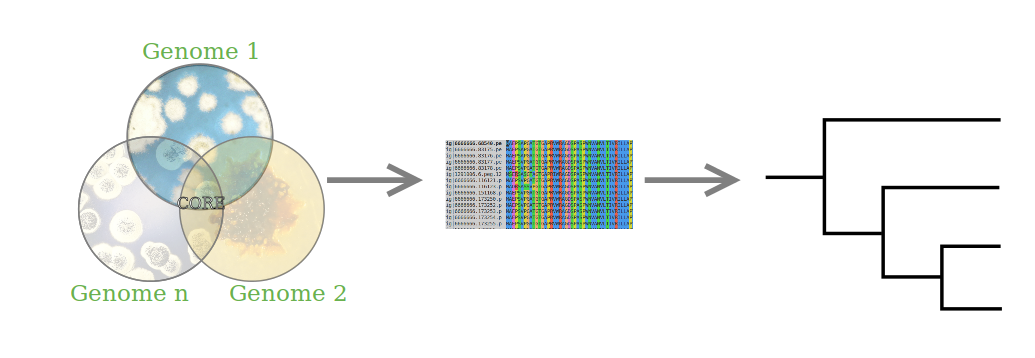
\includegraphics[angle = 0,scale = .42]{chapter1/coreWiki.png}
  \caption[Orthocore calcula el core de un linaje genómico para proveer una filogenia]{\footnotesize{Orthocore calcula las familias génicas comunes de un linaje genómico. Después de un proceso de filtrado, alineamiento y curación concatena estas familias y entrega una reconstrucción filogenética.}}
  \label{fig:Orthocore}
  \end{figure}
  
  El pangenoma es el contenido génico total de un linaje taxonómico. Las
  familias génicas de un pangenoma pueden clasificarse según sus patrones
  de presencia-ausencia en cada genoma del linaje. De acuerdo a esta
  clasificación los principales grupos de familias génicas en un pangenoma
  son el \emph{core}, el \emph{shell} y el \emph{cloud} (dispensable)
  genome. El \emph{core genome} es el conjunto de familias con presencia
  en todos los genomas del linaje. Por ejemplo, la secuencia de la
  subunidad 16s del gene rRNA, así como diversos genes ribosomales que
  suelen estar en el core de la gran mayoría de los linajes bacterianos.
  El \emph{shell genome} es el grupo de familias presentes en la mayoría
  de los genomas pero no en todos. En el \emph{shell} se ubican por
  ejemplo familias que estaban en el \emph{core genome} pero que algunas
  bacterias del linaje sufrieron una dinámica de pérdida (o ganancia)
  génica. Mientras que el \emph{cloud genome} o dispensable genome es
  aquel grupo de familias que sólo ocurre en unos cuantos genomas del
  linaje.
  
  La organización filogenética de un linaje genómico permite la
  observación de pérdida y ganancia de familias génicas en organismos
  cercanos. Si los organismos están desordenados es difícil apreciar la
  dinámica genómica de aparición-desaparición de miembros de una familia
  génica. Ordenar los genomas de un linaje facilita apreciar cambios en el
  número de copias de una familia. Esto es relevante en el marco de esta
  tesis ya que cambios en los perfiles de promiscuidad podrían estar
  relacionados a copias extras de organismos cercanos. Orthocore es un
  algoritmo que utiliza el core conservado de un linaje genómico para
  facilitar la organización filogenética de sus organismos
  \autoref{fig:Orthocore}
  
  \section{La distribución de la función metabólica de las familias del
  pangenoma depende de la variabilidad del linaje
  seleccionado.}\label{la-distribucion-de-la-funcion-metabolica-de-las-familias-del-pangenoma-depende-de-la-variabilidad-del-linaje-seleccionado.}
  
  El número de familias génicas presentes en el pangenoma, así como su
  distribución en el \emph{core}, \emph{shell} y \emph{dispensable genome}
  depende de la elección de los genomas y del linaje genómico. Para
  entender esto se puede pensar en un ejemplo extremo, consideremos una
  bacteria de 1000 familias de genes de la cual se obtienen secuencias de
  diez genomas de la misma cepa. Estas secuenciaciones deberían ser
  prácticamente idénticas y en ese caso el \emph{core genome} sería 1000
  familias, el \emph{shell} y el \emph{dispensable genome} serían cero. En
  este caso, todo el metabolismo, tanto el central como el especializado
  estarían conservados dentro del \emph{core genome}, ya que el
  \emph{shell} y el \emph{dispensable genome} se encuentran vacíos. Sin
  embargo, si variamos el linaje taxonómico, y ahora estudiamos el
  pangenoma de 10 especies distintas del género \emph{Streptomyces} ahora
  el core genome estará compuesto por aproximadamente un tercio de su
  tamaño promedio, y dentro del \emph{core genome} es donde se encontrarán
  muchos de las familias dedicadas al metabolismo central o conservado
  (por ejemplo, familias de la glicólisis o síntesis de aminoácidos). En
  cambio muchas de las familias dedicadas al metabolismo especializado y
  pertenecientes a clústers biosintéticos de productos naturales (BGCs)
  estarán en el \emph{dispensable genome} pues \emph{Streptomyces} es
  productor de una gran variedad de metabolitos especializados y cada
  especie suele tener su producto característico.
  \autoref{fig:MetabolismoPangenoma}
  
  \begin{figure}[h!tbp]
  \centering
  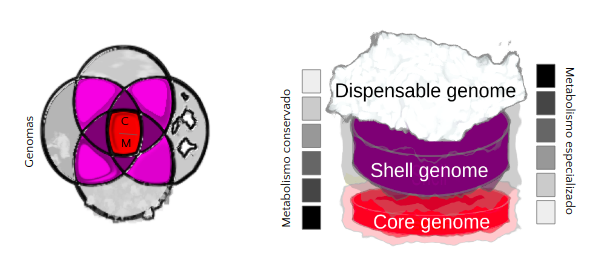
\includegraphics[angle = 0,scale = .75]{chapter1/Metabolismo-Pangenoma.png}
  \caption[El metabolismo en el Pangenoma]{\footnotesize{El pangenoma de un conjunto de genomas de un linaje puede ser clasificado en varios grupos. En este ejemplo, en el lado izquierdo de la figura se observa en gris el $genoma~dispensable$ compuesto por familias génicas presentes sólo en un genoma. En dos tonos de morado observamos el $shell genome$, familias que están presentes en la mayoría de los genomas del linaje, en este en caso dos o tres genomas. Finalmente en rojo se muestra el $core$, aquellas familias presentes en todos los genomas del linaje. El $core$ contiene tanto familias muy conservadas con una sola copia por genoma ( C ), como familias expandidas. Las familias marcadoras (M) pueden ser parte del $core$ conservado o de las familias expandidas. Del lado derecho se muestra una representación del pangenoma para cualquier número de genomas. Familias de metabolismo conservado tenderán a estar concentradas entre el $core$ y el $shell~genome$, mientras que el metabolismo especializado tendrá más representantes en el dispensable que en el $core genome$. Sin embargo tanto el tipo de metabolismo como el tamaño del $core$, $shell$ y $genoma~dispensable$ pueden variar según la diversidad de los organismos seleccionados. }}
  \label{fig:MetabolismoPangenoma}
  \end{figure}
  
  El \emph{core genome} de un linaje, además de tener familias conservadas
  y prácticamente presentes en todo el dominio Bacteria también puede
  contener familias marcadoras \autoref{fig:CoreMarcadores} . Estos genes
  marcadores permiten realizar pruebas de diagnóstico para colonizaciones
  bacterianas. A las familias que están presentes en el \emph{core genome}
  de un linaje A, pero que están completamente ausentes de un linaje B se
  les llama marcadoras. Por ejemplo genes conservados en la especie
  \emph{Streptomyces coelicolor} pero no conservados en \emph{Streptomyces
  rimosus} son genes marcadores de \emph{Streptomyces coelicolor} respecto
  de \emph{Streptomyces rimosus}. Estos mismos marcadores tal vez no sean
  marcadores respecto de \emph{Streptomyces lividans}, a pesar de la
  cercanía taxonómica entre estos organismos. La presencia de genes
  marcadores en el core depende de ambos linajes, por lo que es importante
  contar con algoritmos que permitan automatizar su cálculo.
  
  El número de familias en el pangenoma, ya sea en el \emph{core, shell o
  dispensable} genome no sólo depende de la divergencia o proximidad
  taxonómica de los organismos del linaje seleccionado, también depende de
  lo variable que sea el contenido génico en los genomas del linaje. A
  esta característica se le conoce como apertura. Hay especies, por
  ejemplo algunos patógenos, cuyo pangenoma se encuentra sumamente cerrado
  en el sentido de que no importa cuántos genomas se agreguen, el número
  de familias parece converger y ser asintótico rápidamente a una cota
  superior. En cambio especies o géneros que viven en una gran diversidad
  de hábitats suelen tener un pangenoma abierto. Esto significa que cada
  vez que se agrega un nuevo genoma aparecen otras familias que no estaban
  en los genomas anteriores. En los linajes con pangenoma abierto el
  número de familias nuevas al agregar un genomas seguirá una tendencia
  creciente y no asintótica.
  
  Además de la apertura, existen otros intentos de cuantificar la
  diversidad génica de un linaje. Está por ejemplo la fluidez, definida
  como el promedio de familias únicas entre familias totales por pares de
  genomas. El pangenoma bacteriano total, es decir el total de familias
  génicas en el dominio Bacteria es considerado abierto.
  
  \begin{figure}[h!tbp]
  \centering
  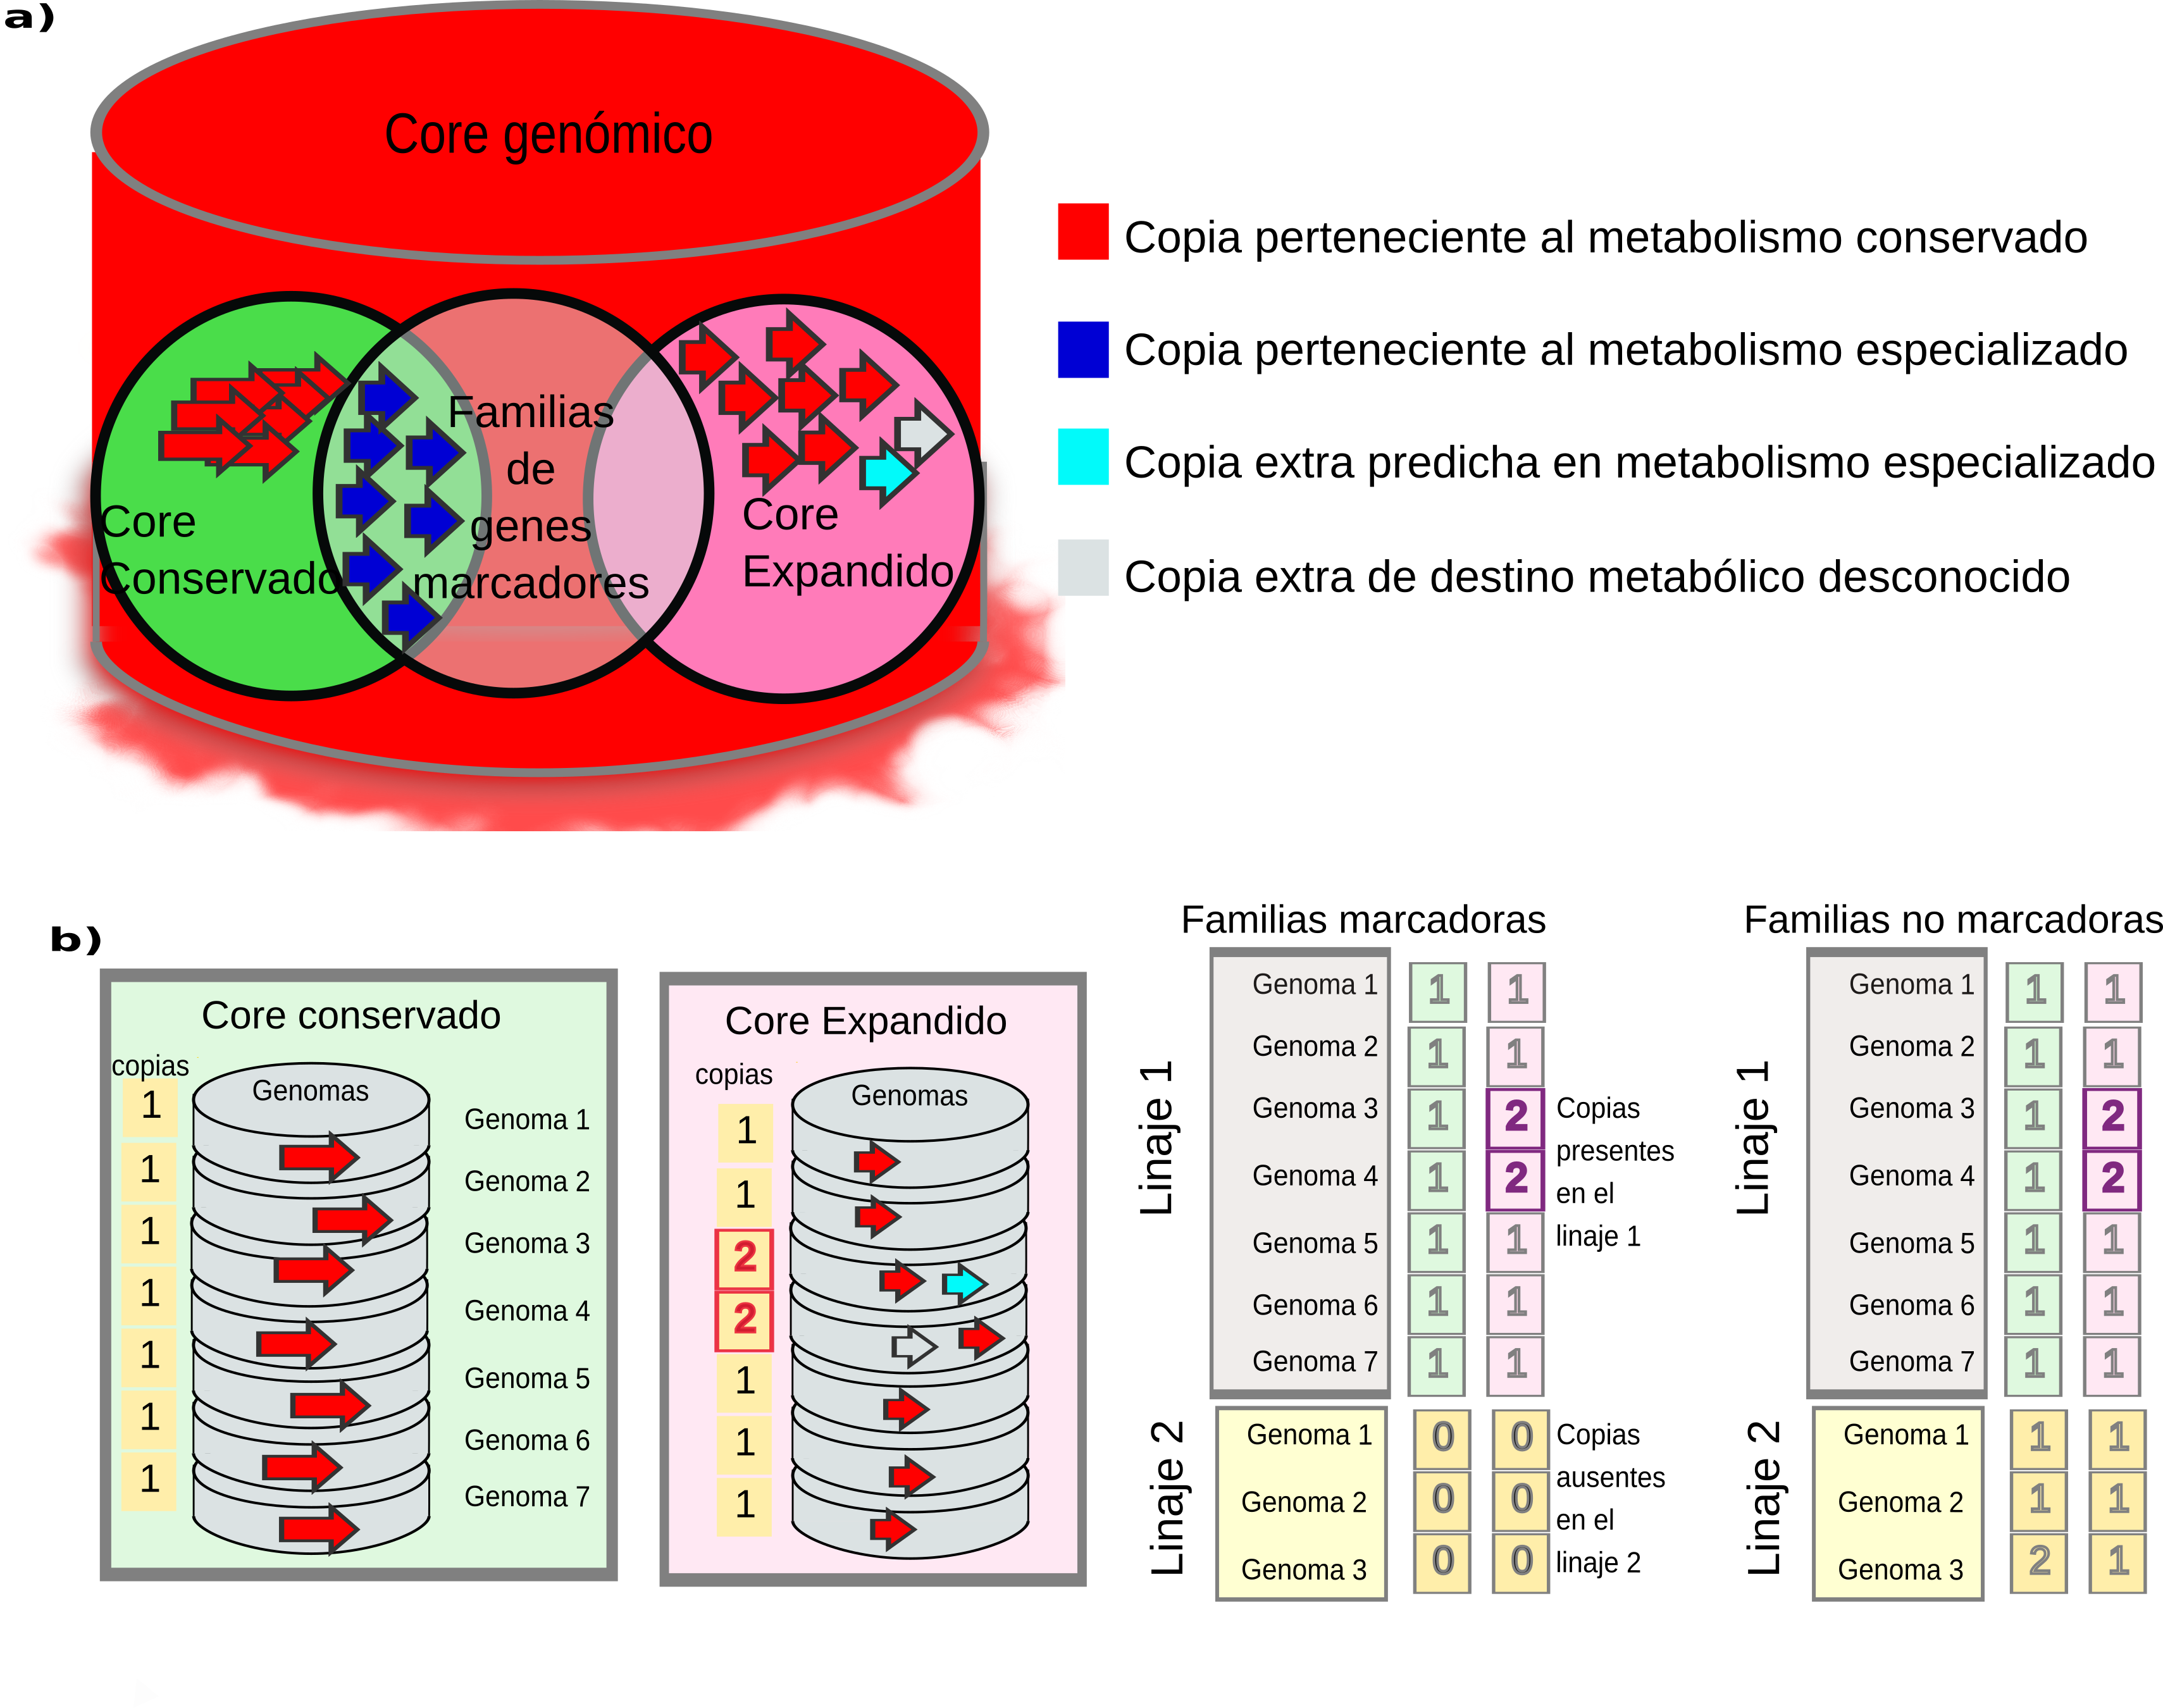
\includegraphics[angle = 0,scale = .8]{chapter1/CoreMarcadores.png}
  \caption[Core y genes Marcadores]{\footnotesize{El core genome puede contener familias con funciones en distintos grupos metabólicos así como diversidad en el número de copias. Arriba se muestra que en el core pueden coexistir familias tanto de copia única como con expansiones. Las familias con funciones en el metabolismo conservado suelen concentrarse en el $core~genome$ (rojas), pero también dependiendo de los organismos seleccionados pueden encontrarse ya sea familias enteras o algunas copias dedicadas al metabolismo especializado (azul). No de todas las copias se conocerá su función, algunas pueden tener un destino metabólico desconocido (gris) o bien ser predichas por algún algoritmo como parte del metabolismo especializado (cyan).  Abajo a la izquierda se comparan familias del $core~conservado$ con exactamente una copia por genoma contra familias del $core~expandido$. Ambas pertenecen al $core$, pero en el $core~expandido$ hay dos genomas que tienen una copia extra en esta familia, unoa cyan y una gris, que podría dificultar la elección de los verdaderos ortólogos. A la derecha se ejemplifican familias de genes marcadores, útiles para identificar un linaje genómico. Tanto familias del $core~conservado$ como del $core~expandido$ pueden ser familias marcadores, siempre que exista al menos una copia de cada familia en el linaje 1 y ninguna copia en el linaje 2. Las familias dejan de ser marcadoras cuando el linaje dos contiene al menos una copia en algún genoma.}}
  \label{fig:CoreMarcadores}
  \end{figure}
  
  Finalmente la distribución de las funciones metabólicas encontrada en
  los subconjuntos del pangenoma ( \emph{core, shell y dispensable}
  genome) está relacionada a la proximidad filogenética de los organismos
  seleccionados en el estudio. Entre más diversos sean los organismos
  menos familias dedicadas exclusivamente a metabolismo especializado
  abundarán en el \emph{core/shell genome}. La diversidad provocará que lo
  único que tengan los genomas de estos organismos en común sean funciones
  conservadas por una amplia variedad de especies bacterianas. Ahora bien,
  muchas familias de metabolismo especializado provienen de reclutamientos
  de copias extra de familias de metabolismo conservado. Así pues aunque
  decrezca el número de familias con exclusividad en metabolismo
  especializado en el \emph{core y shell genome}, estos sunconjuntos del
  pangenoma aún pueden contener familias conservadas que tengan copias
  extra en proceso de reclutamiento para algún Cluster biosintético de
  genes (BGCs) de metabolismo especializado. Considerando las reflexiones
  anteriores, entre más diverso sea un linaje, más tenderá su \emph{core
  genome} a contener exclusivamente familias de metabolismo conservado
  mientras que su dispensable genome estará formado mayormente por
  familias de enzimas del metabolismo especializado.
  
  \section{El core conservado permite la reconstrucción de filogenias
  complicadas}\label{el-core-conservado-permite-la-reconstruccion-de-filogenias-complicadas}
  
  Orthocore es el desarrollo bioinformático que realicé para calcular las
  familias génicas más conservadas del \emph{core genome}. Dos genes son
  homólogos si poseen un ancestro común, entre los principales grupos de
  homólogos están ortólogos y parálogos. Los ortólogos provienen de
  eventos de especiación de un ancestro común mientras que los parálogos
  evolucionan por eventos de duplicación. Orthocore obtiene un subconjunto
  del \emph{core genome}: el \emph{core conservado}, es decir, familias de
  ortólogos presentes en todos los genomas del grupo y que además son
  libres de parálogos de difícil identificación. El \emph{core conservado}
  facilita la organización en árboles filogenéticos de organismos de un
  linaje genómico.
  
  La comparación de la variación molecular entre ortólogos ha sido
  utilizada para establecer relaciones filogenéticas entre organismos.
  Esta técnica ha dado lugar a grandes descubrimientos. Por ejemplo
  comparar la secuencia de la subunidad 16s del gene RNA ribosomal condujo
  a Woese al descubrimiento del dominio Archaea en 1977
  {[}\protect\hyperlink{ref-woese_phylogenetic_1977}{124}{]}. Un árbol de
  especies suele hacerse con secuencias de familias que pertenecen al core
  genome de un Dominio, por ejemplo las familias 16s o RpoB en los
  Dominios Bacteria y Archaea. Algunos autores realizan árboles multilocus
  para mejorar la resolución de árboles de especies realizados mediante la
  comparación de secuencias de 16s. Los genes seleccionados para los
  árboles multilocus deben estar en todos los organismos y no tener copias
  extra tan parecidas que puedan confundirse y entorpecer la
  reconstrucción filogenética, es decir, las familias seleccionadas deben
  ser parte del \emph{core conservado}. Orthocore automatiza la
  identificación de estas familias.
  
  Entre los factores importantes para establecer las relaciones
  filogenéticas diferenciando entre Archaea y Bacteria están los
  siguientes: 1) la presencia conservada de la subunidad de 16s en los
  tres dominios mencionados, y 2) la suficiente divergencia entre estas
  secuencias en los organismos de dichos dominios. Ahora bien, establecer
  relaciones filogenéticas entre Archaea y Bacteria es en cierto sentido
  más sencillo que establecerlas entre organismos pertenecientes al mismo
  género o inclusive a la misma especie. En ocasiones, como en el caso del
  género \emph{Streptomyces}, la secuencia de 16s por sí sola no posee la
  suficiente variación para resolver la filogenia
  {[}\protect\hyperlink{ref-labeda_phylogenetic_2017}{140}{]}. En
  \emph{Streptomyces} la variación entre estas secuencias suele ser menor
  al 1\%. Para resolver el problema de escasa variación en secuencias de
  16s se pueden concatenar las secuencias de otros ortólogos, siempre que
  estos aparezcan en todos los organismos que se estén estudiando, es
  decir, siempre que sean parte del core genómico.
  
  \section{El algoritmo de Orthocore}\label{el-algoritmo-de-orthocore}
  
  \begin{figure}[h!tbp]
  \centering
  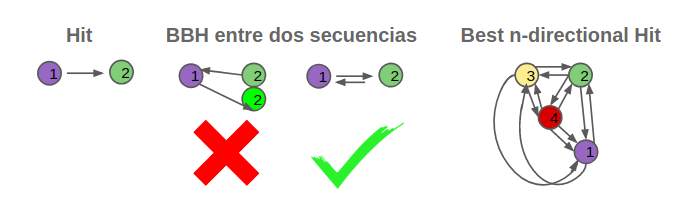
\includegraphics[angle = 0,scale = .55]{chapter1/Best-n-directional.png}
  \caption[Los mejores hits n-direccionales generalizan a los $Bidirectional~Best~Hits$]{\footnotesize{Orthocore utiliza los mejores hits n-direccionales para obtener grupos de ortólogos. Un hit es el mejor resultado de una secuencia en otro genoma. Un Bidireccional Best Hit es el mejor hit bidireccional. La secuencia 2 es el mejor hit de la secuencia 1 en el genoma 2 y recíprocamente, la secuencia 1 es el mejor hit de la secuencia 2 en el genoma 1. La existencia de una copia extra muy parecida a la secuencia 2 puede romper el BBH. Un mejor hit n-direccional debe ser BBH todos contra todos garantizando que estas secuencias están muy conservadas entre sí.}}
  \label{fig:Best-n-directional}
  \end{figure}
  
  Los ortólogos suelen identificarse por similitud de secuencia, pero si
  se realiza la identificación manualmente también se suelen capturar
  parálogos que pueden confundir la elucidación de eventos de especiación.
  Orthocore automatizó la búsqueda de ortólogos y el filtrado de parálogos
  en genomas procariontes mediante la generalización de la definición del
  mejor hit bidireccional (BBH por sus siglas en inglés)
  \autoref{fig:Best-n-directional} . Dos secuencias son BBH si cada una es
  el mejor hit de un algoritmo de distancia (BLAST usualmente) en el
  genoma de origen de la otra. Una primera generalización para obtener el
  set de ortólogos de una familia del core es definir un genoma de
  referencia y tomar los BBH respecto a ese genoma. En la práctica, esta
  definición da como resultado distintos resultados según el genoma de
  referencia, haciendo que algunos parálogos no sea filtrados.
  
  Para solventar esta dificultad se definió en Orthocore el concepto de
  mejores hits multidireccionales. Un conjunto de genes son mejores hits
  multidireccionales si todos entre sí son BBH por pares. Es decir si cada
  gen fuera un punto y ser mejor hit se expresara como una conexión con
  dirección todos los puntos estarían conectados por una flecha de ida y
  otra de regreso. Con este método se eliminó la dependencia de un genoma
  de referencia. Esta restricción también ocasiona que en grupos muy
  grandes por ejemplo más de 100 genomas de distintas especies, o muy
  diversos de distintos dominios, o muy fragmentados como con contigs de
  en promedio 3 Mbp, el core conservado puede quedar vacío.
  
  \subsection{Componentes técnicos de
  Orthocore}\label{componentes-tecnicos-de-orthocore}
  
  Orthocore es un tubería escrita en perl que incorpora los hits
  multidireccionales permitiendo obtener y usar el core conservado para
  realizar una reconstrucción filogenética mediante los siguientes pasos:
  
  -Obtiene el core conservado: los mejores n-direcional hits (blastp).\\
  -Alinea cada familia del core conservado (MUSCLE).\\
  -Cura automáticamente cada familia del core conservado (Gblocks).\\
  -Concatena las familias del core conservado formando una matriz de
  aminoácidos.\\
  -Realiza una reconstrucción filogenética de la matriz de aminoácidos
  (FastTree)\\
  -Provee las funciones del core conservado según la anotación funcional
  de RAST.
  
  Existen otros algoritmos como OrthoMCL, y fastOrtho que dividen
  pangenomas en clusters de familias de genes, get\_homologues y metaphor
  que obtienen el core y filtran buscando verdaderas relaciones de
  homología, y finalmente BPGA que hace reconstrucciones filogenéticas
  tanto según el core como según el pangenoma. Sin embargo Orthocore
  resolvió en su momento la necesidad específica de proporcionar una
  matriz concatenada de genes del core conservado lista para utilizarse en
  un árbol multilocus. Adicionalmente, como Orthocore fue diseñado para
  trabajar con la anotación de la plataforma RAST, también se obtiene la
  anotación funcional tanto de familias del core como del complemento.
  
  Orthocore incorpora todas las dependencias en un contenedor de docker
  disponible en \url{https://github.com/nselem/orthocore}. Además en este
  contenedor está un script que permite bajar genomas de NCBI masivamente
  y posteriormente anotarlos en RAST desde la terminal. Los protocolos de
  uso se encuentran al final de este capítulo.
  
  \subsection{Aplicaciones de Orthocore, identificación del core
  conservado y de familias de genes
  marcadores.}\label{aplicaciones-de-orthocore-identificacion-del-core-conservado-y-de-familias-de-genes-marcadores.}
  
  Cuatro aplicaciones de Orthocore serán presentadas en las siguientes
  secciones de este capítulo. En la primera aplicación el core conservado
  en \emph{Actinomycetales} permitió organizar filogenéticamente a este
  orden. Esta organización facilitó el entendimiento en cambios de
  promiscuidad de la familia enzimática PriA mediante la distinción de
  patrones de pérdida y ganancia de genes en las rutas de síntesis de
  histidina y triptófano. En la segunda aplicación cepas de
  \emph{Salmonella tifi} fueron ordenadas filogenéticamente. La tercera
  aplicación permitió realizar una reconstrucción filogenética del orden
  \emph{Nostocales} del phylum \emph{Cyanobacteria} y comparar así
  patrones de presencia y ausencia de clusters de genes biosintéticos.
  Finalmente, en organismos del microbioma del tomate orthocore de utilizó
  para identificar genes marcadores que permitieran distinguir cepas de
  \emph{Clavibacter Michiganensis} de otras especies de
  \emph{Micrococcales}.
  
  Perfiles de promiscuidad de PriA en el orden \emph{Actinomycetales} se
  relacionan con la especiación. Para mejorar el entendimiento de los
  cambios en promiscuidad enzimática de PriA, se necesitaba entender
  filogenéticamente al orden \emph{Actinomycetales}, un camino era obtener
  su core conservado. Orthocore fue diseñado para resolver este problema.
  Con el resultado de Orthocore se realizó un árbol de especies donde se
  observaron patrones de pérdida y ganancia de genes en la vecindad
  genómica del gen que codifica para PriA. Se encontró que hay clados de
  \emph{Actinomyces} donde los genes correspondientes a la síntesis de
  histidina no estaban en la vecindad genómica de PriA, y mediante la
  realización de cinéticas enzimáticas se comprobó que la actividad de
  catalizar la reacción correspondiente a HisA estaba perdida en estos
  organismos. A estas enzimas se les llamó subTrpF ya que sólo poseían la
  capacidad de catalizar la reacción correspondiente a la familia TrpF.
  Del mismo modo existían clados que perdieron los genes de síntesis de
  triptófano en la vecindad de PriA y estas enzimas se subfuncionalizaron
  a la familia subHisA. De estos datos se observa que en estos organismos
  la especiación coincidió con el cambio de promiscuidad en la familia
  PriA, acorde a la pérdida y ganancia de genes vecinos. La promiscuidad
  puede co-ocurrir con variaciones en el contexto genómico, pudiendo estos
  cambios ser una marca para sugerir cambio funcional en una familia.
  
  \subsection{\texorpdfstring{Genes de islas de patogenicidad de
  \emph{Salmonella} en México están conservados en la mayoría de los
  genomas.}{Genes de islas de patogenicidad de Salmonella en México están conservados en la mayoría de los genomas.}}\label{genes-de-islas-de-patogenicidad-de-salmonella-en-mexico-estan-conservados-en-la-mayoria-de-los-genomas.}
  
  Para estudiar la diversidad de \emph{Salmonella} presente en alimentos
  en México, primero se ensamblaron y anotaron genomas secuenciados para
  el trabajo ``distribución de los genes de la toxina VirB/D4 en plásmidos
  de bovino asociados a \emph{Salmonella} no tifoidal''. Los genomas
  fueron ensamblados en Patrick y se desarrolló myRAST, una tubería previa
  a Orthocore para la anotación automática de genomas ensamblados en RAST.
  El protocolo de myRAST puede encontrarse al final de este capítulo.
  
  Orthocore fue usado aquí para reconstruir filogenias de
  \emph{Salmonella} y además fue integrado como parte de CORASON, el cual
  se reporta en el Capítulo 3, es el algoritmo que sirve para visualizar
  variantes de clusters organizados filogenéticamente. Los clusters de
  genes pueden ser biosintéticos, islas de patogenicidad, operones o
  cualquier región parcialmente sinténica de un genoma bacteriano centrada
  en un gen. En este caso se observó una alta conservación de toxinas
  tifoidales en islas de patogenicidad de \emph{Salmonella}. Éstas fueron
  identificadas en 76\% de las cepas analizadas y posteriormente
  visualizadas mediante CORASON.
  
  \subsection{Nostoc provenientes del metagenoma de cícadas se agrupan
  Cyanobacteria}\label{nostoc-provenientes-del-metagenoma-de-cicadas-se-agrupan-cyanobacteria}
  
  \begin{figure}[h!tbp]
  \centering
  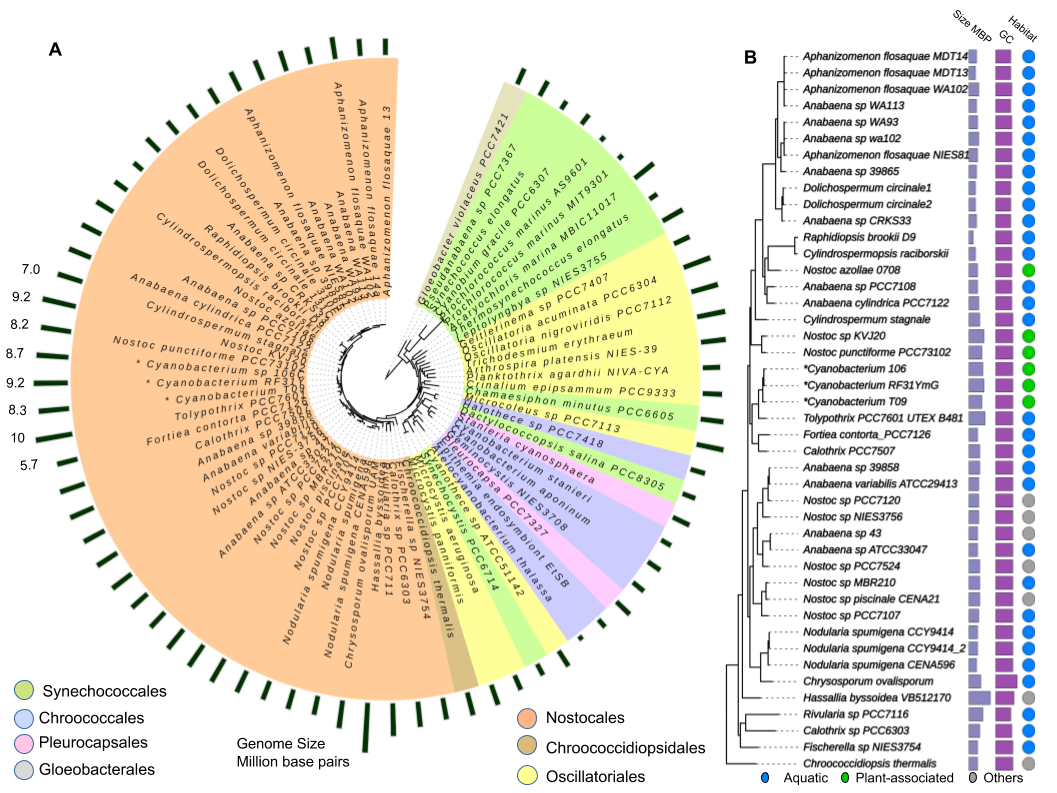
\includegraphics[angle = 0,scale = .45]{chapter1/Nostoc.png}
  \caption[Arbol filogenético de $Nostoc$ construido utilizando  la selección de genes del $core~conservado$]{\footnotesize{Reconstrucción de 76 taxa provenientes de 7 órdenes de Cyanobacteria. La matriz final incluyó 45,475 aminoácidos curados de 198 familias de proteínas pertenecientes al $core~conservado$. A la derecha se muestra un zoom sobre el orden $Nostocales$. En este orden se incluyen algunas bacterias simbiontes de cícadas. Metadatos como el tamaño de genoma, contenido de GC y hábitat de origen muestran una posible tendencia de incremento de tamaño en los genomas provenientes del microbioma de plantas.}}
  \label{fig:ArbolNostoc}
  \end{figure}
  
  Las Cyanobacterias son un phylum de bacterias que se han adaptado a
  diversos ambientes. Aunque muchas de ellas son marinas algunas
  Cyanobacterias viven como simbiontes de plantas. En particular las
  cícadas han desarrollado un tipo especial de raíz donde se sabe que vive
  como simbionte el género \emph{Nostoc}. La presencia de \emph{Nostoc} en
  la raíz coraloide de las cícadas es fácilmente distinguible por la
  formación de un anillo verde conocido como anillo cyanobacterial. En la
  \autoref{fig:ArbolNostoc} se muestra la filogenia de 76 Cyanobacterias
  de 7 órdenes distintos construida con 198 proteínas del core conservado
  obtenidas por Orthocore. En esta reconstrucción se puede observar que
  los \emph{Nostoc} asociados a plantas tienden a agruparse en la
  filogenia.
  
  \subsection{Identificación de genes marcadores de Clavibacter
  michiganensis}\label{identificacion-de-genes-marcadores-de-clavibacter-michiganensis}
  
  \emph{Micrococcales} es un orden de Actinobacteria que contiene a
  \emph{Clavibacter}, \emph{Micrococcus} y \emph{Microbacterium}, entre
  otros microorganismos. El género \emph{Clavibacter} comprende especies
  que pueden causar enfermedades en diversas plantas. En particular la
  especie \emph{Clavibacter michiganensis} es una bacteria causante de la
  enfermedad del cáncer del tomate. \emph{Clavibacter michiganensis} ha
  sido frecuentemente aislada en compañía de otros \emph{Micrococcales}
  morfológicamente parecidos. La distinción entre microorganismos debida a
  la comparación de la secuencia de 16s no era suficiente para distinguir
  entre \emph{Micrococales} del microbioma del tomate, por lo que una
  prueba de diagnóstico se hacía necesaria. Se habían utilizado como
  marcadores genes como \emph{tomA}, \emph{ppaC} y \emph{celA} entre
  otros, sin embargo estas elecciones en ocasiones resultaban en falsos
  positivos según árboles de especies de 16s, por lo que nuevos marcadores
  eran necesarios.
  
  \begin{figure}[h!tbp]
  \centering
  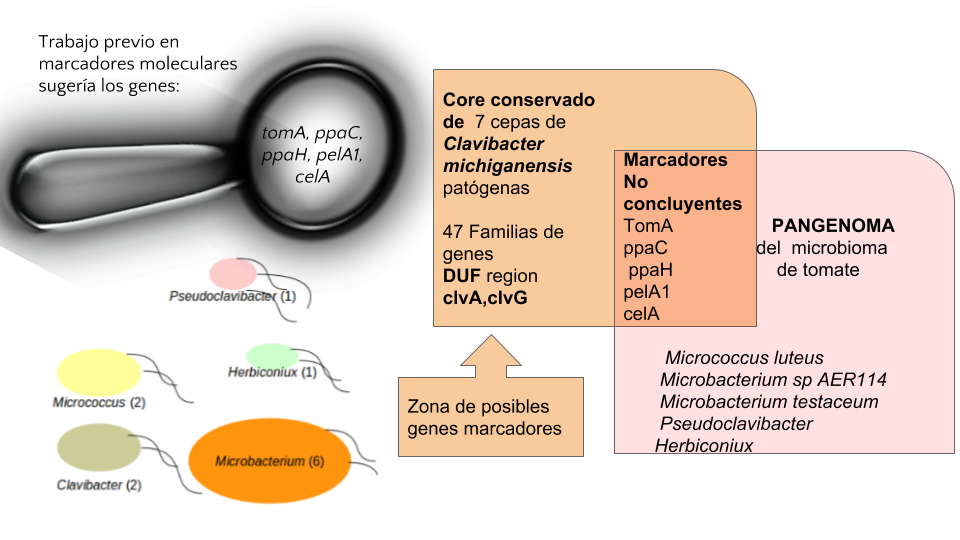
\includegraphics[angle = 0,scale = .5]{chapter1/Marcadores-Clavibacter.png}
  \caption[Los genes del cluster biosintético clv son marcadores de $Clavibacter$]{\footnotesize{Los marcadores moleculares previos a este trabajo no permitían diferenciar correctamente a $Clavibacter~michiganensis$ respecto al microbioma del tomate en invernaderos mexicanos. Arriba a la izquierda se muestran los antiguos marcadores $tomA, ppaC, ppaH, pelA1, celA$. Abajo organismos pertenecientes al microbioma del tomate. Orthocore obtuvo el core conservado de siete cepas de $Cmm$ patógenas, y este core se utilizó para definir nuevos marcadores. Aunque $tomA$ pertenecía al core conservado de $Cmm$, estaba también incluido en el pangenoma del microbioma del tomate. Después de calcular la intersección core conservado de $Cmm$ y pangenoma del microbioma se obtuvieron entre las familias marcadoras genes $clv$ parte del cluster biosintético de clavidicina (michiganina).}}
  \label{fig:Marcadores}
  \end{figure}
  
  Al analizar en RAST genomas de \emph{Microbacterium} y
  \emph{Micrococcus} aislados de tomate se encontró que en efecto,
  \emph{tomA} y los otros marcadores propuestos previamente no eran
  exclusivos de \emph{Clavibacter michiganensis} ( \emph{Cmm} ). Al
  utilizar Orthocore en siete genomas de \emph{Cmm} encontramos que varios
  genes del cluster biosintético de michiganina (BGC0000528 en MIBiG)
  codificado por los genes \emph{clvAFGLKM} pertenecían al core
  conservado, pero que al agregar los genomas no Cmm del resto del
  microbioma del tomate los genes \emph{clv} se pierden. El descubrimiento
  de que \emph{clv} pertenecía al core de \emph{Cmm} se realizó con
  secuencias de genomas muy fragmentados, en la\autoref{fig:Marcadores} se
  muestran las cepas originales que fueron analizadas.
  
  \begin{figure}[h!tbp]
  \centering
  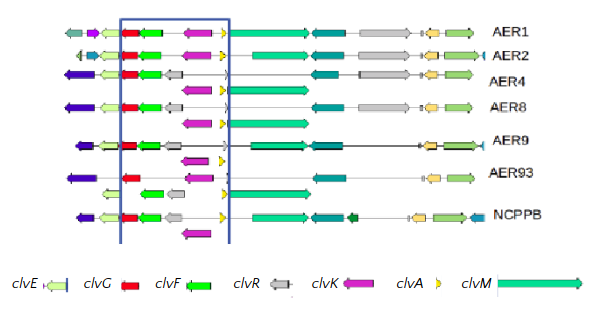
\includegraphics[angle = 0,scale = .6]{chapter1/clv.png}
  \caption[ clv BGC]{\footnotesize{clavibacter}}
  \label{fig:clv-Marcadores}
  \end{figure}
  
  Esta observación se corroboró con más genomas,
  \autoref{fig:clv-Marcadores} en este caso se muestran como ejemplo 10
  genomas de bacterias del microbioma del tomate, entre ellas siete
  \emph{Clavibacter}, seis de tomates de invernadero y uno
  \emph{Clavibacter} proveniente de tomate silvestre, \emph{Clavibacter}
  RA1B que fue reportado en la tesis de maestría de Yanez. Con Orthocore
  vemos que el tamaño del core decrece al ir agregando genomas de
  \emph{Clavibacter} y decrece aún más rápido al agregar los genomas de
  \emph{Micrococcus} y \emph{Microbacterium} La reconstrucción
  filogenetica de este microbioma, ubica a \emph{Clavibacter} RA1B cerca
  de los otros \emph{Cmm} pero no en un clado junto con ellos. Una
  búsqueda por blast revela que los genes marcadores de \emph{Cmm}:
  \emph{clvF}, \emph{clvR} son también marcadores de \emph{Clavibacter}
  RA1B pero no así \emph{clvA} y \emph{clvG} que solamente están presentes
  en el core de \emph{Cmm}. Sin embargo \emph{clvF} y \emph{clvR} no están
  en el contexto del cluster de michiganina en RA1B y su similitud de
  secuencia es menor que la que se observa entre los otros \emph{Cmm}.
  
  De hecho al considerar más genomas dentro del microbioma del tomate, la
  familia \emph{clvF} no solo no está en el core conservado de
  \emph{Microbacterium} y \emph{Micrococcus}, sino que no está presente en
  ningún otro genoma distinto a \emph{Clavibacter}. Con distintos niveles
  de conservación de secuencia los genes \emph{clv} son un buen marcador
  para distinguir \emph{Cmm} de otras especies, por esta razón estos genes
  aún se encuentran en uso como genes marcadores de \emph{Cmm}. Esta misma
  conclusión se reporta en el trabajo de yasuhara, su observación de que
  las familias \emph{clvA, clvF} y \emph{clvG} son exclusivas de
  \emph{Cmm} es independiente de la nuestra, fue hecha sin análisis
  genómicos y basada en evidencia experimental
  {[}\protect\hyperlink{ref-yasuhara-bell_genes_2014}{141}{]}. Este
  descubrimiento ha permitido bajar los costos de identificación de
  Clavibacter, ya que ahora en lugar de enviar a secuenciar el genoma es
  suficiente identificar por PCR \emph{clvF} en conjunto con otro
  marcadores.
  
  Con Orthocore además de obtener los genes marcadores podemos obtener
  también la matriz del core conservado para realizar la reconstrucción
  filogenética de especies cercanas de \emph{Clavibacter}. Debido a que es
  importante para los agricultores conocer de dónde provienen las
  bacterias que infectan al tomate, una de las líneas de investigación del
  laboratorio de evolución de la diversidad metabólica, es la organización
  taxonómica de cepas de \emph{Cmm} y de otras bacterias del microbioma de
  tomate. Por este motivo se tienen unos doscientos genomas privados y se
  esperan más a futuro. Orthocore colabora con esta investigación
  proporcionando matrices multilocus que pueden diferenciar entre
  \emph{Clavibacter} de la misma o de diferente especie.
  
  \begin{figure}[h!tbp]
  \centering
  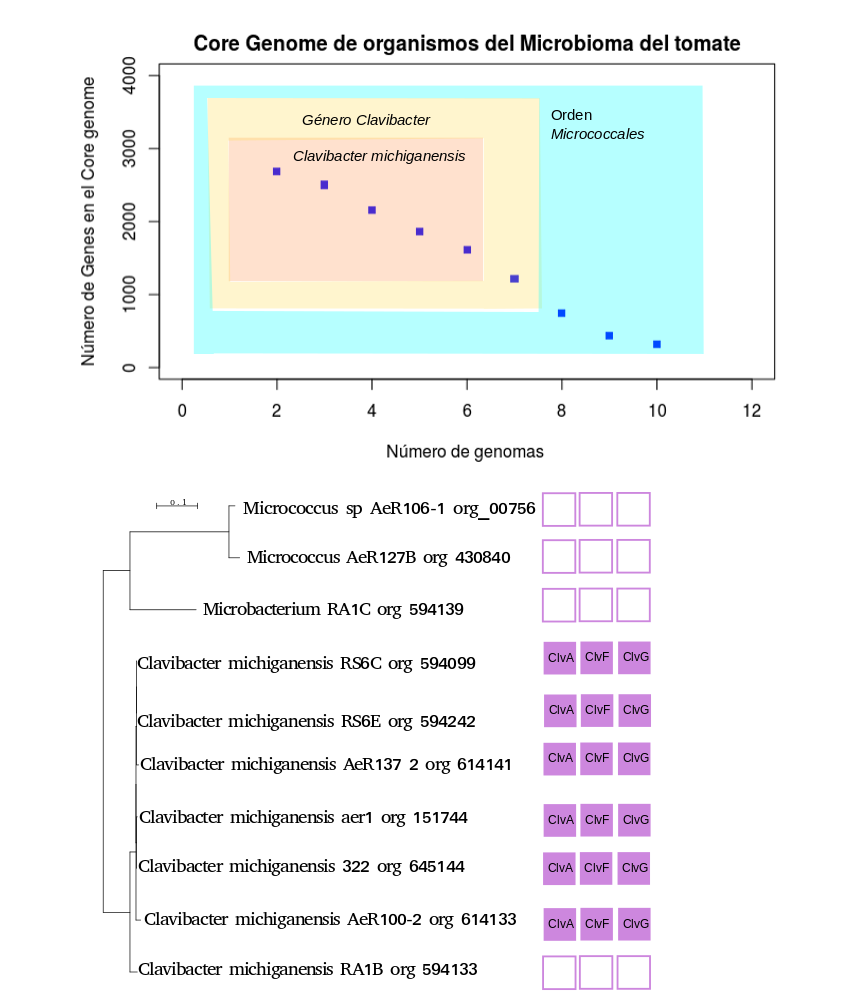
\includegraphics[angle = 0,scale = .5]{chapter1/CoreGenomeMicrobioma.png}
  \caption[ X X Evomining]{\footnotesize{Aqui vemos los marcadores de EEvomining}}
  \label{fig:Clavibacter-EvoMining}
  \end{figure}
  
  Debido al intercambio génico por transferencia horizontal en las
  bacterias, es posible que los genes marcadores actuales alguna vez
  aparezcan en otros organismos. También las bacterias pierden
  continuamente genes, por lo que es posible que algún gen marcador de Cmm
  se pierda en una cierta cepa \autoref{fig:Clavibacter-EvoMining} . Esto
  hace que la definición de estar presentes en el core del grupo de
  interés y ausentes totalmente de cada uno de los genomas de otro linaje
  ya no funcione completamente. Sin embargo, en estas dos situaciones
  presentadas, ganancia de genes marcadores de organismos externos al
  linaje original o pérdida de genes marcadores en algunas cepas, se sigue
  cumpliendo que los ex genes marcadores, estarán presentes en la mayoría
  de los organismos del linaje de interés y ausentes de la mayoría de los
  organismos del linaje externo. Por ello, se pensó que está definición de
  genes marcadores se podía generalizar clasificando a grupos de genes
  ortólogos acorde a sus porcentajes de ocurrencia. Esta idea se
  desarrolló en la herramienta clavisual, explicada en la siguiente
  sección.
  
  \section{Clavisual: Identificación de genes marcadores a un cierto
  porcentaje de grupos
  seleccionados}\label{clavisual-identificacion-de-genes-marcadores-a-un-cierto-porcentaje-de-grupos-seleccionados}
  
  La idea de que Orthocore puede ser usado para obtener los genes
  marcadores de un grupo taxonómico frente a otro fue generalizada en el
  backend del software Clavisual. Ya se ha explicado previamente que el
  core puede salir vacío por diversas razones, entre ellas baja calidad de
  los genomas, o que éstos provengan de organismos muy divergentes,
  verdaderas razones biológicas como dinámica génica o un core no
  convergente. Así pues, es posible que si sólo se utiliza el core no se
  obtengan marcadores. Pero el core puede relajarse de varias maneras una
  de ellas es el Pseudocore, donde en lugar de multidireccional hits se
  toman BBH a un genoma de referencia. Otra forma es establecer un
  porcentaje de presencia /ausencia de interés.
  
  El pseudocore consiste en \_\_\_\_\_\_\_\_ y la metodología está
  depositada en github en el repositorio\_\_\_\_\_\_\_\_\_. El blast fue
  optimizado cambiando hacer un blast todos contra todos por archivos
  genómicos individuales genomai\_vs\_genomaj.blast que luego son
  concatenandos según se necesiten.
  
  Los porcentajes de genomas son diferentes porque al no bastar los best
  bidireccional hits conservados, todo el pangenoma es decir todos los
  genes contenidos en los genomas del grupo de interés necesitan ser
  clasificados por familias, para de ahi obtener las familias que tienen
  presencia en un porcentaje \%p y ausencia en un porcentaje a\% del grupo
  externo. Estos perfiles fueron desarrollados para Clavisual
  \autoref{fig:Clavisual} utilizando FasthOrtho para clasificar las
  familias y de ahi obtener los grupos. Con ellos se consiguieron
  marcadores para Kurtobacterium.
  
  Finalmente Clavisual despliega un árbol realizado con el Pseudocore
  respecto a un conjunto de genes de Cmm NCPP previamente seleccionados.
  En este árbol clavisual permite la visualización de metadatos, como año,
  género de la bacteria, estado de salud de la planta e invernadero donde
  fue aislada.
  
  \begin{figure}[h!tbp]
  \centering
  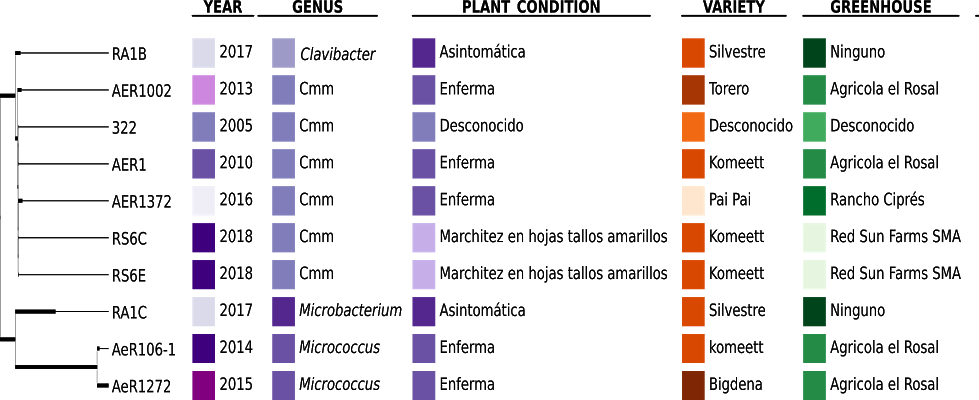
\includegraphics[angle = 0,scale = .4]{chapter1/Clavisual.png}
  \caption[ X X XXXX]{\footnotesize{Aqui vemos un arbol}}
  \label{fig:Clavisual}
  \end{figure}
  
  \subsection{El pangenoma de Clavibacter Michiganensis es
  abierto}\label{el-pangenoma-de-clavibacter-michiganensis-es-abierto}
  
  Después de desarrollar métodos de identificación de genes marcadores y
  generalizarlo a obtener grupos con patrones de presencia/ausencia
  definidos por el usuario, quedaba por responder la pregunta cómo es el
  pangenoma de \emph{Cmm}. Algunos autores consideran que el pangenoma de
  patógenos es reducido porque sus genomas suelen sufrir proceso de
  reducción de tamaño débido a la pérdida de genes. Como \emph{Cmm} es un
  patógeno de planta quedaba por investigar cómo es su pangenoma. ¿Es
  posible saturar el contenido génico de \emph{Cmm} con sólo secuenciar
  más genomas?. Aunque actualmente existen ya herramientas web para el
  análisis de pangenoma, en su momento se utillizó el software bpga que se
  corre desde la terminal. Para facilitar su instalación se desarrolló un
  docker que se describe más tarde en este capítulo en la sección de las
  descripciones técnicas. Como ejemplo de su funcionamiento, se analizó el
  pangenoma de los mismos diez genomas del pangenoma del tomate utilizados
  en la visualización de clavisual \autoref{fig:bpga-pangenoma} .
  
  \begin{figure}[h!tbp]
  \centering
  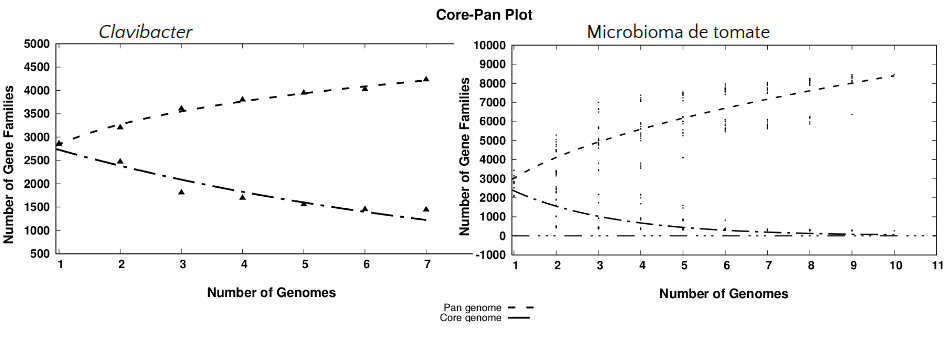
\includegraphics[angle = 0,scale = .5]{chapter1/bpga-pangenoma.png}
  \caption[ X X]{\footnotesize{adihipihfd }}
  \label{fig:bpga-pangenoma}
  \end{figure}
  
  Tomando otros siete clavibacters, utilizando OrthoVenn tenemos la misma
  observación, el número de familias de genes agregadas al adicionar
  genomas, es después de siete genomas casi tan grande como su core
  \autoref{fig:Venn-Chart}.
  
  \begin{figure}[h!tbp]
  \centering
  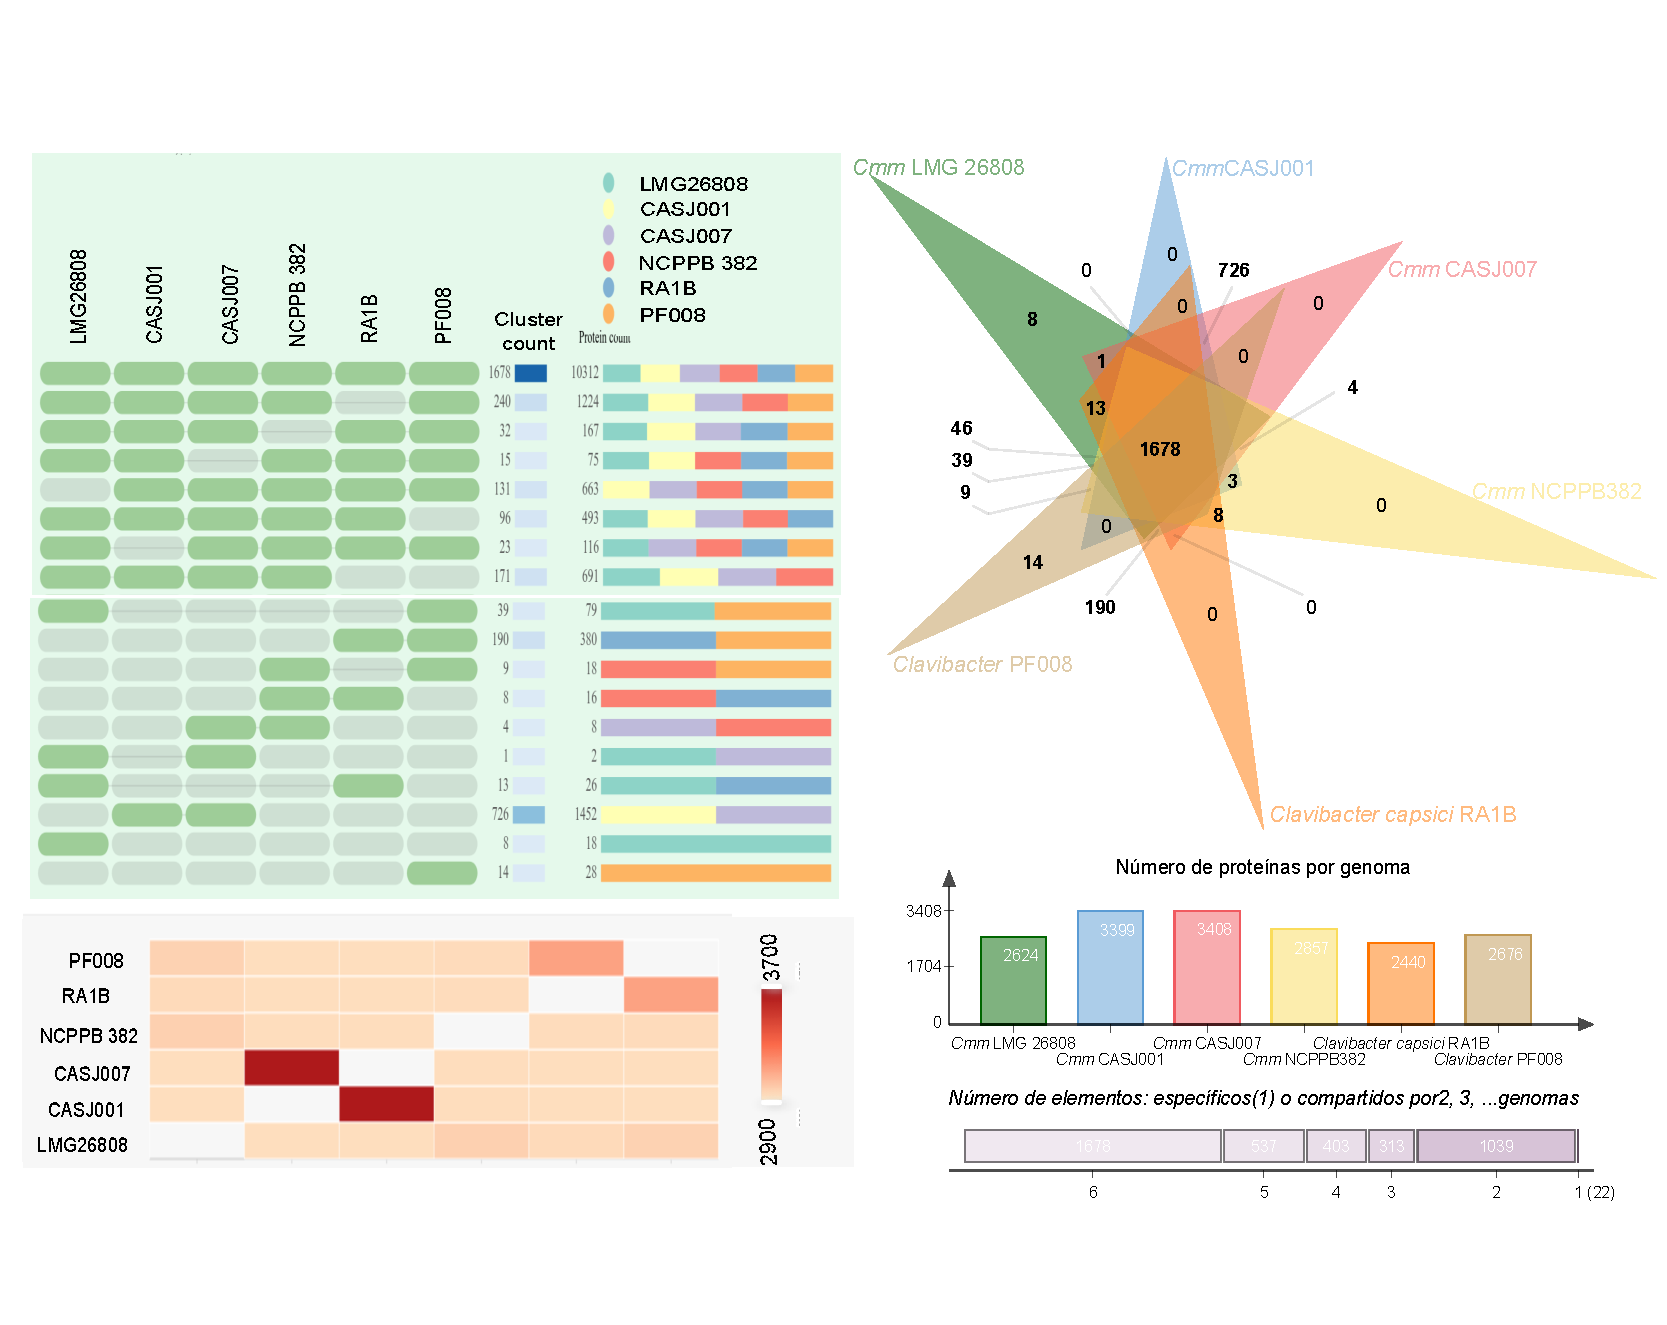
\includegraphics[angle = 0,scale = .6]{chapter1/Venn_chart.pdf}
  \caption[ X X]{\footnotesize{Diagrama de Venn del pangenoma de Clavibacter Selectos}}
  \label{fig:Venn-Chart}
  \end{figure}
  
  \section{Relación entre genes marcadores, Orthocores y la promiscuidad
  enzimática.}\label{relacion-entre-genes-marcadores-orthocores-y-la-promiscuidad-enzimatica.}
  
  Finalmente, al aplicar Orthocore para detectar genes marcadores se
  vuelve indirectamente reclutamientos al metabolismo especializado, cómo,
  pues porque dentro de los marcadores hay productos naturales como,
  PENDIENTE VER RESULTADOS RETRO-EVOMINING la clavidicina (michiganina).
  Ahí vemos que clvABCDEF participan en metabolismo secundario, las
  enzimas de metabolismo central de este cluster pueden presentar cierta
  promiscuidad.
  
  \section{Protocolos para usar Orthocore, myRAST, fastOrtho,
  Clavigenomics, y
  BPGA}\label{protocolos-para-usar-orthocore-myrast-fastortho-clavigenomics-y-bpga}
  
  Anotación genómica con el docker myRAST
  
  Esta es una distribución de myRAST en un contenedor de docker. Para
  usarla se necesita una cuenta del anotador genómico RAST. el docker
  myRAST permite hacer anotación genómica y funcional masiva mediante el
  uso de la terminal en el anotador RAST. Después de anotar los resultados
  pueden descargarse y procesarse en una terminal
  
  Descargar myrast docker distribution
  
  Una vez con docker instalado en la computadora, se hace pull al docker
  myrast.
  
  docker pull nselem/myrast\\
  Abrir myRast en la terminal
  
  docker run -i -t -v \$(pwd):/home nselem/myrast /bin/bash
  
  Usar myRast
  
  -Ejemplo subir un archivo fasta
  
  svr\_submit\_RAST\_job -user -passwd -fasta -domain Bacteria -bioname
  ``Organism name'' -genetic\_code 11 -gene\_caller rast
  
  -Para bajar un archivo de anotación genómica funcional:
  
  svr\_retrieve\_RAST\_job table\_txt \textgreater{} \$ID.txt
  
  Una lista completa de archivos puede ser procesada usando bash. Por
  ejemplo para bajar una lista de archivos de RAST se deben guardar los
  identificadores de RAST en una columna de un archivo, (Rast\_ID en este
  ejemplo) y usar un while para obtenerlos:
  
  En este caso la variable ``line'' contendrá el identificador RAST Id, y
  cada archivo fasta de aminácidos podrá ser obtenido mediante su
  identificador de RASTy será guardado en el archivo ``\$line.faa''
  
  cut -f1 Rast\_ID \textbar{} while read line; do svr\_retrieve\_RAST\_job
  \$line amino\_acid \textgreater{} \$line.faa ; done\\
  Formatos de RAST para descargar archivos
  
  Puedes cambiar el formato table\_txt por el que tú necesites.
  
  \begin{longtable}[]{@{}ll@{}}
  \caption{Formatos de descarga disponibles en myRAST
  \label{tab:myrast}}\tabularnewline
  \toprule
  \begin{minipage}[b]{0.22\columnwidth}\raggedright\strut
  Atributo\strut
  \end{minipage} & \begin{minipage}[b]{0.72\columnwidth}\raggedright\strut
  Descripción\strut
  \end{minipage}\tabularnewline
  \midrule
  \endfirsthead
  \toprule
  \begin{minipage}[b]{0.22\columnwidth}\raggedright\strut
  Atributo\strut
  \end{minipage} & \begin{minipage}[b]{0.72\columnwidth}\raggedright\strut
  Descripción\strut
  \end{minipage}\tabularnewline
  \midrule
  \endhead
  \begin{minipage}[t]{0.22\columnwidth}\raggedright\strut
  genbank\strut
  \end{minipage} & \begin{minipage}[t]{0.72\columnwidth}\raggedright\strut
  GenBank (con funciones y enriquecimiento de SEED)\strut
  \end{minipage}\tabularnewline
  \begin{minipage}[t]{0.22\columnwidth}\raggedright\strut
  genbank\_stripped\strut
  \end{minipage} & \begin{minipage}[t]{0.72\columnwidth}\raggedright\strut
  Genbank con EC-numbers removidos de las funciones\strut
  \end{minipage}\tabularnewline
  \begin{minipage}[t]{0.22\columnwidth}\raggedright\strut
  embl\strut
  \end{minipage} & \begin{minipage}[t]{0.72\columnwidth}\raggedright\strut
  EMBL (con funciones y enriquecimiento de SEED)\strut
  \end{minipage}\tabularnewline
  \begin{minipage}[t]{0.22\columnwidth}\raggedright\strut
  embl\_stripped\strut
  \end{minipage} & \begin{minipage}[t]{0.72\columnwidth}\raggedright\strut
  EMBL con EC-numbers removidos de las funciones\strut
  \end{minipage}\tabularnewline
  \begin{minipage}[t]{0.22\columnwidth}\raggedright\strut
  gff3\strut
  \end{minipage} & \begin{minipage}[t]{0.72\columnwidth}\raggedright\strut
  GFF3\strut
  \end{minipage}\tabularnewline
  \begin{minipage}[t]{0.22\columnwidth}\raggedright\strut
  gff3\_stripped\strut
  \end{minipage} & \begin{minipage}[t]{0.72\columnwidth}\raggedright\strut
  GFF3 con EC-numbers removidos de las funciones\strut
  \end{minipage}\tabularnewline
  \begin{minipage}[t]{0.22\columnwidth}\raggedright\strut
  gtf\strut
  \end{minipage} & \begin{minipage}[t]{0.72\columnwidth}\raggedright\strut
  GTF\strut
  \end{minipage}\tabularnewline
  \begin{minipage}[t]{0.22\columnwidth}\raggedright\strut
  gtf\_stripped\strut
  \end{minipage} & \begin{minipage}[t]{0.72\columnwidth}\raggedright\strut
  GTF con EC-numbers removidos de las funciones\strut
  \end{minipage}\tabularnewline
  \begin{minipage}[t]{0.22\columnwidth}\raggedright\strut
  rast\_tarball\strut
  \end{minipage} & \begin{minipage}[t]{0.72\columnwidth}\raggedright\strut
  Archivo comprimido (gzipped) con todo el directorio de las anotaciones
  de RAST sobre el genoma\strut
  \end{minipage}\tabularnewline
  \begin{minipage}[t]{0.22\columnwidth}\raggedright\strut
  nucleic\_acid\strut
  \end{minipage} & \begin{minipage}[t]{0.72\columnwidth}\raggedright\strut
  Fasta de DNA de genes\strut
  \end{minipage}\tabularnewline
  \begin{minipage}[t]{0.22\columnwidth}\raggedright\strut
  amino\_acid\strut
  \end{minipage} & \begin{minipage}[t]{0.72\columnwidth}\raggedright\strut
  Fasta de DNA de aminoácidos\strut
  \end{minipage}\tabularnewline
  \begin{minipage}[t]{0.22\columnwidth}\raggedright\strut
  table\_txt\strut
  \end{minipage} & \begin{minipage}[t]{0.72\columnwidth}\raggedright\strut
  Gene data in tab-separated format\strut
  \end{minipage}\tabularnewline
  \begin{minipage}[t]{0.22\columnwidth}\raggedright\strut
  table\_xls\strut
  \end{minipage} & \begin{minipage}[t]{0.72\columnwidth}\raggedright\strut
  Preserve the original gene calls and use RAST\strut
  \end{minipage}\tabularnewline
  \bottomrule
  \end{longtable}
  
  Referencia \autoref{tab:myrast}.
  
  \section{Orthocore}\label{orthocore}
  
  El umbral de e-value de Orthocore es por default 1e-6. Todas las
  secuencias son alineadas usando MUSCLE v3.8.31 con los parámetros
  default y curadas utilizando Gblocks con 5 posiciones como longitud
  mínima del bloque, 10 como máximo número de posiciones contiguas no
  conservadas y sólo considerando posiciones con gaps menores que el 50\%
  de las secuencias en el alineamiento final. Después de esta curación las
  secuencias son concatenadas en una matriz final.
  
  \chapter{EvoMining como herramienta para identificar el origen y el
  destino metabólico de familias
  enzimáticas}\label{evomining-como-herramienta-para-identificar-el-origen-y-el-destino-metabolico-de-familias-enzimaticas}
  
  \section{Introducción}\label{introduccion-1}
  
  La promiscuidad enzimática puede buscarse en familias envueltas en
  procesos de divergencia funcional. Uno de dichos procesos es la
  expansión y posterior reclutamiento de familias pertenecientes a rutas
  metabólicas conservadas hacia el metabolismo especializado. Los
  productos naturales o metabolitos especializados son sintetizados
  generalmente por clusters de genes distribuidos en un pequeño porcentaje
  de un linaje taxonómico. Estos clusters, conocidos como BGCs
  (Biosynthetical Gene Clusters), contienen reclutamientos de las copias
  extras de familias pertenecientes al metabolismo conservado. La
  similitud de secuencia de los genes que pertenecen a los BGCs así como
  su relativa sintenia en diversos organismos de un linaje hacen que
  genómica copmarativa sea de utilidad para intentar localizarlos.
  Finalmente, el auge en la cantidad de genomas disponibles públicamente
  así como la facilidad por sequenciar nuevos hace posible que los métodos
  bioinformáticos ayuden a encontrar nuevos BGCs. EvoMining es un método
  de para sugerir la formación de nuevos BGCs y en consecuencia encontrar
  zonas donde puede estar ocurriendo la capcidad de adquirir un nuevo
  sustrato cambio en promiscuidad enzimátcica.
  
  En este capítulo se explica el desarrollo de EvoMining como plataforma
  bioinformática dedicada a presentar una visualización del origen y
  destino de todas las copias de familia enzimátocas provenientes del
  emtabolismo conservado. Se discutirán también cuatro linajes genómicos
  Actinobacteria Cyanobacteria, \emph{Pseudomonas} y Archaea y finalmente
  se analizará un BGCs scytonemin.
  
  \section{EvoMining es un método para encontrar BGCs no
  tradicionales}\label{evomining-es-un-metodo-para-encontrar-bgcs-no-tradicionales}
  
  Existen varias clases de BGCs que son arquetipos de los productos
  naturales. Entre ellas se encuentran las clases \emph{non ribosomomal
  peptide synthase} (NRPS), \emph{poliketide synthase} PKS, terpenos,
  RIPPs, alcaloides, etc. En estas clases, hay enzimas cuya presencia
  lleva a la detección del BGC. Por ejemplo, las sintasas no ribosomales
  son las que al encontrarlas dan nombre a los BGC tipo NRPS y las
  policétido sintasas son las que dan nombre a los BGC de la clase PKS.
  
  \begin{figure}[h!tbp]
  \centering
  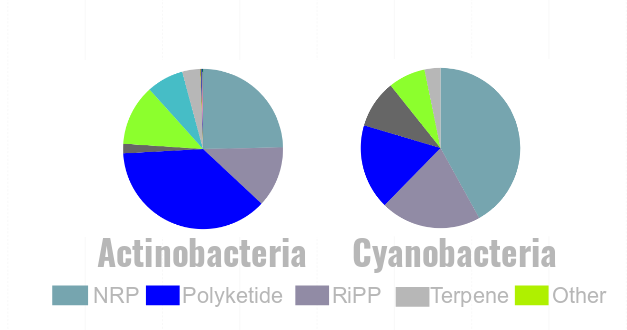
\includegraphics[angle = 0,scale = .7]{chapter2/other.png}
  \caption[Existen cluster biosintéticos no clasificados (other) entre los reportados en MIBiG]{\footnotesize{Existen cluster biosintéticos no clasificados (other) entre los reportados en MIBiG}}
  \label{fig:other}
  \end{figure}
  
  No todos los productos naturales están dentro de los BGCs clásicos.
  Dentro de MIBiG hay 231 BGC (\(12.7\%\)) clasificados como ``otros'',
  que de hecho carecen de PKS, NRPS o cualquiera de las otras clases de
  enzimas características del metabolismo especializado. Como ejemplo se
  muestra la \autoref{fig:other} donde se aprecia que un porcentaje de los
  BGC reportados tanto en Actinobacteria como en Cyanobacteria pertenece
  al grupo ``otros''. La ausencia de enzimas biosintéticas conocidas hace
  que estos BGC sean ``atípicos'', difíciles de identificar. Los BGC no
  clasificados suelen pasar desapercibidos, porque no hay conocimiento
  previo de ellos que permita reconocerlos. Por ello EvoMining busca
  implementar una estrategia de búsqueda de divergencia del metabolismo
  conservado en lugar de la estrategia de búsqueda de similitud con
  metabolismo especializado. La ramas divergentes en el registro de
  secuencias analizadas a través de la evolución son una herramienta para
  la búsqueda de secuencias divergentes del metabolismo conservado.
  
  Localizar alguna enzima de un cluster no clasificado es un camino para
  identificar el BGC. Como ya se mostró en EvoMining 1.0 encontramos una
  enzima que XXX Un ejemplo de este escenario es el BGC de scytonemin
  {[}\protect\hyperlink{ref-garciapichel_evidence_1992}{142}{]},protector
  solar cianobacteriano, que incluye ScyB y ScyA como las dos enzimas
  biosintéticas clave que sostienen la síntesis de este metabolito
  especializado
  {[}\protect\hyperlink{ref-balskus_investigating_2008}{143}{]}.
  
  Curiosamente, ScyB y ScyA son homólogos distantes de la glutamato
  deshidrogenasa (GDH) y la acetolactato sintasa (ALS), respectivamente,
  que participan en la desaminación oxidativa reversible del glutamato a
  \(\alpha-\)ketoglutarato y amoníaco
  {[}\protect\hyperlink{ref-engel_glutamate_2014}{145}{]} y en la síntesis
  de cadena ramificada aminoácidos
  {[}\protect\hyperlink{ref-liu_acetohydroxyacid_2016}{146}{]},
  respectivamente.
  
  \subsection{Copias extra de familias enzimáticas que son reclutadas para
  una nueva función están relacionadas con la
  promiscuidad.}\label{copias-extra-de-familias-enzimaticas-que-son-reclutadas-para-una-nueva-funcion-estan-relacionadas-con-la-promiscuidad.}
  
  Algunas retienen la función ancestral mientras que las ancestrales
  comienzan a desarrollar la nueva función.
  
  \begin{figure}[h!tbp]
  \centering
  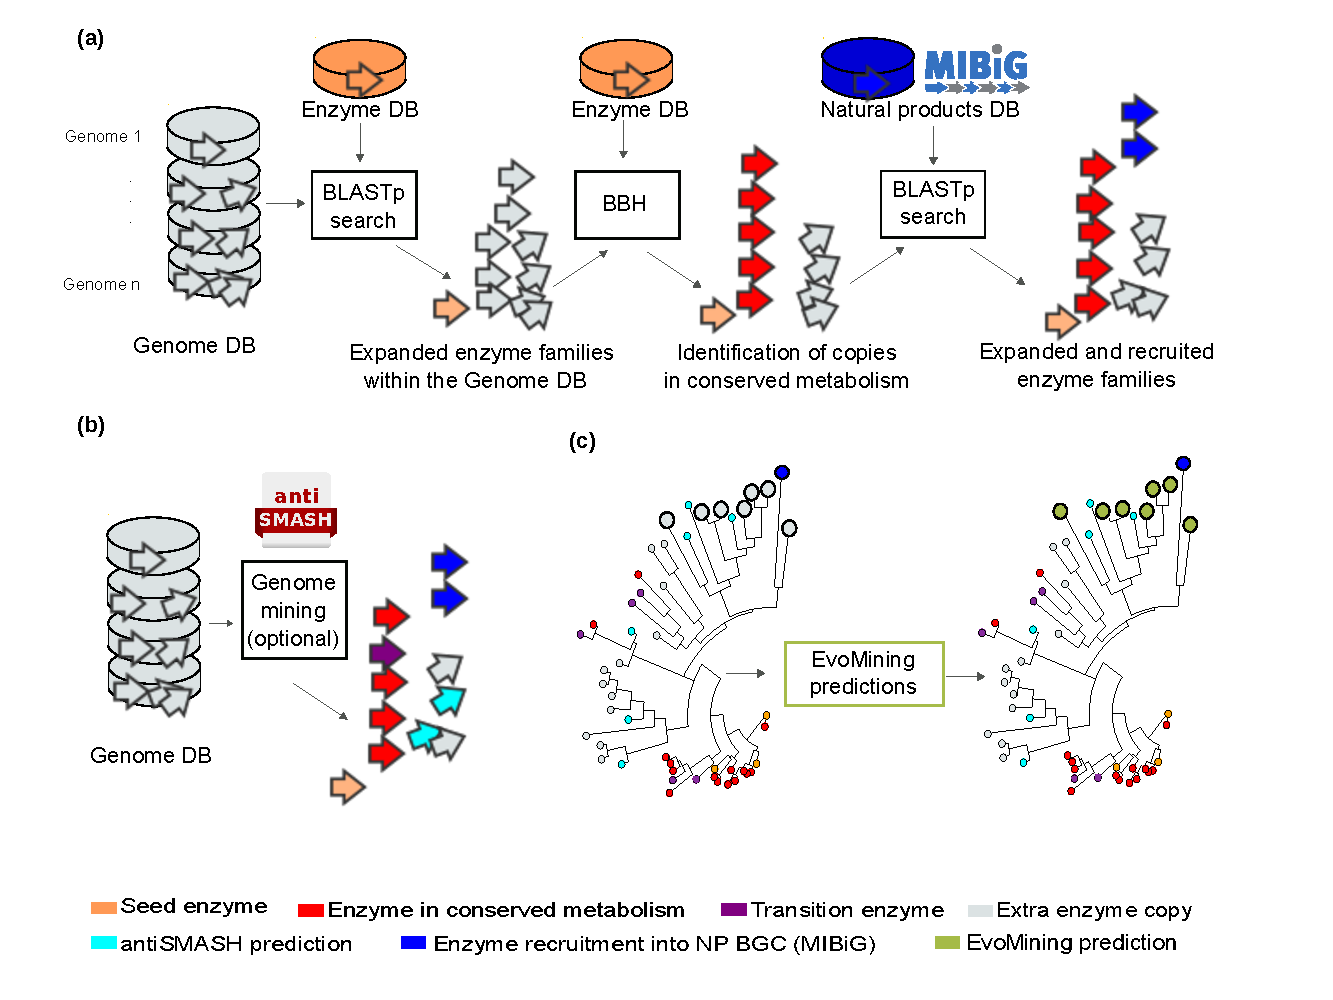
\includegraphics[angle = 0,scale = .7]{chapter2/FigurasPaper/Figure1.pdf}
  \caption[EvoMining Algorithm]{\footnotesize{}}
  \label{fig:EvoMiningAlgorithms}
  \end{figure}
  
  \subsection{EvoMining es un paradigma que permite ubicar copias extra de
  familias enzimáticas y organizarlas visualmente acorde a eventos
  evolutivos.}\label{evomining-es-un-paradigma-que-permite-ubicar-copias-extra-de-familias-enzimaticas-y-organizarlas-visualmente-acorde-a-eventos-evolutivos.}
  
  \section{Algoritmos y bases de datos de EvoMining
  2.0}\label{algoritmos-y-bases-de-datos-de-evomining-2.0}
  
  EvoMining está compuesto de dos algoritmos, el de búsqueda de patrones
  de expansión - reclutamiento y el de visualización de todas las copias
  de una familia expandida clasificadas según sus posibles destinos
  metabólicos. Además de los algortimos EvoMining necesita tres bases de
  datos: i) la genómica, ii) las semillas enzimáticas, y iii) la de
  productos naturales.
  
  \subsection{Algoritmo de expansión y
  reclutamiento}\label{algoritmo-de-expansion-y-reclutamiento}
  
  La primera parte de la minería genómica evolutiva de EvoMining consiste
  en detectar las expansiones y los reclutamientos de las familias
  enzimáticas semilla. Una familia expandida consiste en todas las copias
  detectadas mediante una búsqueda con BLASTp, e-value de 0.001 y bitscore
  de 100, usando como query las secuencias de aminoácidos de las enzimas
  semilla (Enzyme DB) y como base de datos de búsqueda las secuencias de
  genomas de un linaje taxonómico (Genome DB). Un reclutamiento es una
  copia extra de una familia de metabolismo conservado que ahora participa
  en metabolismo especializado. Ejemplos de reclutamientos conocidos han
  sido observados en BGCs reportados en MIBiG. Ejemplos de reclutamientos
  predichos se encuentran en enzimas pertenecientes a BGCs reconocidos por
  antiSMASH que tienen un origen en metabolismo conservado.
  
  En la primera versión de nuestro trabajo definimos que un organismo
  poseía una expansión si el número de copias de una familia estaba por
  encima del promedio mas dos desviaciones estándar. Siguiendo esta
  definición EvoMining colorea en un heat plot las expansiones de las
  familias enzimáticas respecto a un linaje taxonómico, señalando
  explícitamente el número de copias de cada familia.
  
  En este sentido, no todas ls copias son expansiones, pero aún así pueden
  ser predicciones de EvoMining, por ello para futuros trabajos es posible
  que estar una unidad arriba de la moda, sea suficiente para ser un
  reclutamiento.
  
  Los patrones de reclutamiento sólo pueden ser apreciados tras ordenar
  los organismos filogenéticamente, por ejemplo \emph{Streptomyces} tiene
  dos enolasas. Se recomienda al usuario reordenar los organismos del
  heatplot de acuerdo a un árbol de especies, mismo que puede ser
  calculado utilizando Orthocore.
  
  En este paso, en cada familia expandida los ortólogos más parecidos a
  las enzimas semilla de la enzyme DB son identificados por BBH. Estos
  ortólogos serán considerados parte del metabolismo conservado y serán
  posteriormente identificados con color rojo en la visualización. Las
  copias extra parte de la familia expandida son enzimas de las que no se
  conoce el destino metabólico, es posible que en los pasos subsequentes
  de EvoMining sean reconocidas por antiSMASH o EvoMining como posibles
  reclutamientos a metabolismo especializado. En otro caso permanecerán
  como copias extra con destino metabólico desconocido.
  
  Una vez obtenidas las FEs expandidas e identificado los ortólogos del
  metabolismo central, se conduce una nueva búsqueda con BLASTp, E-value
  0.001, utilizando las EFs como queries contra la base de datos NP DB, la
  de enzimas biosintéticas presentes en BGCs. Otras bases de datos que
  contengan enzimas con un destino metabólico conocido podrían utilizarse
  en lugar de NP DB. Los reclutamientos son la
  
  En conclusión el algoritmo de expansión - reclutamiento trabaja para
  identificar tres clases de copias en las familias enzimáticas expandidas
  (i) copias altamente conservadas con algún miembro en el metabolismo
  conservado; (ii) reclutamientos conocidos en BGCs de productos
  naturales; y (iii) copias extra que no son reclutamientos conocidos ni
  parte obvia del metabolismo conservado, quedando por definir su destino
  metabólico. Reconstrucciones filogenéticas de las familias enzimáticas
  serán utilizadas en la siguiente sección para asignar a estas copias
  extra obtenidas por el algoritmo de expansión y reclutamiento un origen
  y destino metabólico
  
  \begin{figure}[h!tbp]
  \centering
  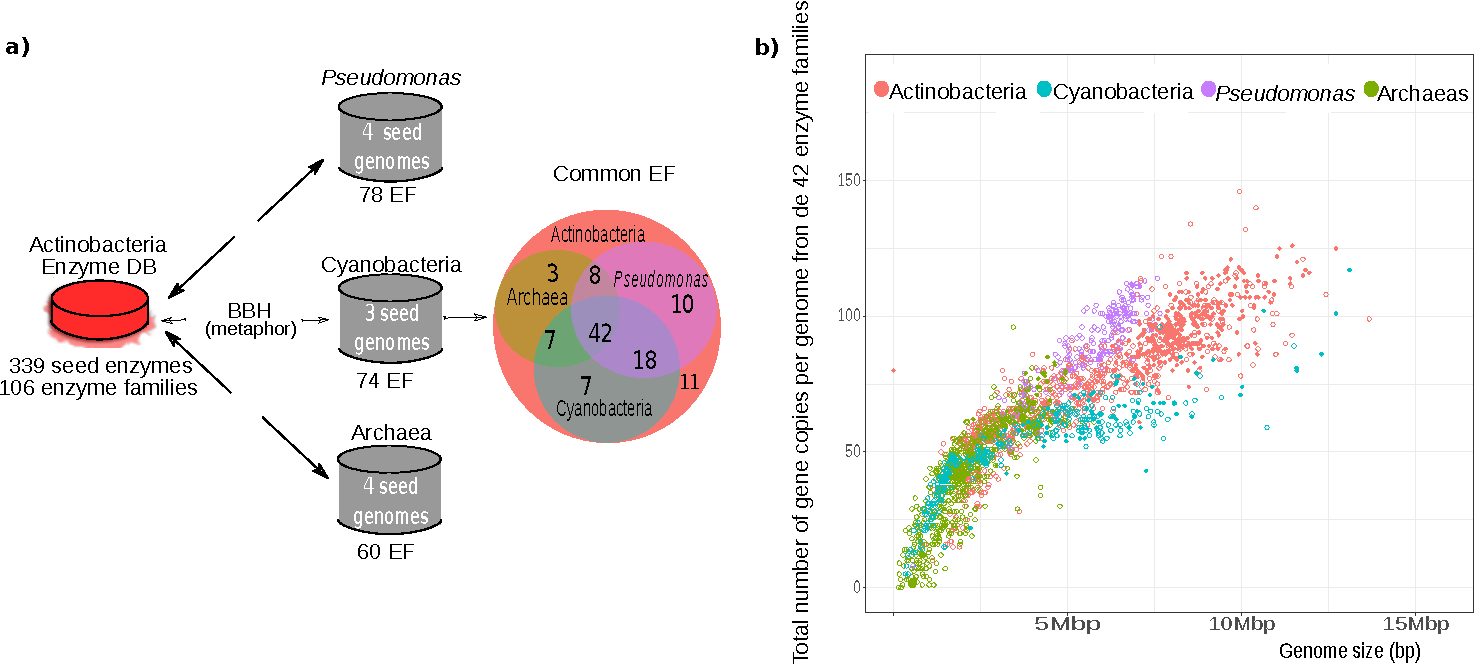
\includegraphics[angle = 0,scale = .6]{chapter2/FigurasPaper/Figure2.pdf}
  \caption[Seed genomes]{\footnotesize{}}
  \label{fig:SeedGenomes}
  \end{figure}
  
  \subsection{Algoritmo de reconstrucción filogenética y
  visualización}\label{algoritmo-de-reconstruccion-filogenetica-y-visualizacion}
  
  Las secuencias de las familias enzimáticas expandidas fueron alineadas
  con muscle v3.2{[}\protect\hyperlink{ref-edgar_muscle_2004}{147}{]} y
  curadas con Gblocks
  v0.91b{[}\protect\hyperlink{ref-castresana_selection_2000}{148}{]}. Los
  parámetros de Gblocks fueron fijados en incluir 5 posiciones como el
  mínimo tamaño de un bloque y diez posiciones como el máximo de
  posiciones contiguas no conservadas. Posiciones ausentes de más del
  \(50\%\) de las secuencias fueron filtradas y removidas del alineameinto
  final. Para recontruis filogenéticamente la historia de las enzimas se
  utilizó FastTree
  \(2.1\){[}\protect\hyperlink{ref-price_fasttree_2010}{149}{]} que es un
  método muy rápido pensado para miles de secuencias que utiliza un
  algoritmo definido como ``aproximadamente máxima verosimilitud''.
  
  La minería genómica tradicional realizada por antiSMASH no es parte de
  la tubería de EvoMining, pero puede las predicciones de antiSMASH pueden
  ser calculadas previamente por el usuario y utilizadas por EvoMining. En
  este trabajo antiSMASH
  3.0{[}\protect\hyperlink{ref-weber_antismash3_2015}{150}{]} fue
  utilizado en los secuencias de los genomas de la Genome DB
  \autoref{fig:EvoMiningAlgorithms} panel (b).
  
  La selección de color de las hojas del árbol fue automatizada utilizando
  Newick Utilities una serie de programas llamados desde la terminal para
  manipular árboles en formato
  Newick{[}\protect\hyperlink{ref-junier_newick_2010}{151}{]}. La
  anotación funcional de RAST en su versión
  clásica{[}\protect\hyperlink{ref-aziz_rast_2008}{86}{]} fue agregada al
  SVG. Otros metadatos como el número de copias por organismo y fueron
  escritos de manera que los árboles producidos por EvoMining sean
  compatible con la visualización de
  Microreact{[}\protect\hyperlink{ref-argimon_microreact_2016}{152}{]}.
  
  Los árboles de EvoMining diferencian entre la función metabólica de cada
  miembro de una familia génica mediante un código de color
  \autoref{fig:EvoMiningAlgorithms} panel (b, c) . Las secuencias más
  conservadas se identifican mediante BBH contra la Enzyme DB, los hits de
  este proceso son considerados copias de metabolismo central, y son
  marcadas en rojo. En el otro extremo están los reclutamientos conocidos
  con alguna evidencia experimental que fueron reportados en
  MIBiG{[}\protect\hyperlink{ref-medema_minimum_2015}{105}{]}. Estos
  reclutamientos son marcados en azul. Una vez definidos estos dos grupos,
  una predicción de EvoMining es definida como aquellas hojas más cerca de
  una hoja azul que de una hoja roja. Estas predicciones consideradas con
  más posibilidades de pertenecer al metabolismo especializado que al
  conservado, son coloreadas en verde \autoref{fig:EvoMiningAlgorithms}
  panel (c).
  
  Además de los tres destinos metabólicos descritos marcados
  respectivamente en rojo, azul y verde, se puede opcionalmente agregar
  información predicha por antiSMASH. Cuando el usuario provee resultados
  de antiSMASH sobre qué genes pertenecen a un BGC que contiene una enzima
  típica de metabolismo especializado, estos se colorean en cyan y son
  llamados predicciones antiSMASH. Si una secuencia es al mismo tiempo
  predicción EvoMining y predicción antiSMASH se colorea cyan y se ignora
  el verde para enfatizar en los verdes las posibles novedades químicas.
  Cuando una secuencia está en la intersección de las reconocidas como
  metabolismo conservado marcada como roja y predicción de antiSMASH es
  decir color cyan entonces es coloreada de púrpura. Estas enzimas de
  intersección entre metabolismo conservado y metabolismo especializado
  son definidas como enzimas de intersección. Finalmente para todas las
  copias extra que no fueron marcadas como rojas, azules, verdes, cyanes o
  púrpuras existe el color girs. Así pues gris son aquellas hojas del
  árbol de las que no se tiene un clave sobre su destino metabólico, estas
  secuencias son llamadas de destino metabólico desconocido.
  
  \subsection{Las tres bases de datos de
  EvoMining}\label{las-tres-bases-de-datos-de-evomining}
  
  EvoMining DBs Tres bases de datos son requeridas como variables de
  inicio de EvoMining, la primera es el conjunto de secuencias de genomas
  de un linaje, esta base fue llamada Genome DB. La segunda es un grupo de
  secuencias de enzimas de metabolismo conservado llamada Enzyme DB. La
  base de datos se secuencias de genes que pertenecen a un cluster
  biosintético de metabolismo especializado es abreviada como base de
  datos de productos naturales o por sus siglas en inglés NP DB. Las
  transformaciones que sufrieron estas bases de datos desde la primera
  versión de EvoMining hasta este trabajo están resumidas en la tabla uno
  y serán descritas a continuación( Table 1 ).
  
  Genome DB La primera versión de Genome DB comprendió 230 genomas de
  Actinobacteria, incluyendo 50 géneros diferentes. Gracias a la explosión
  de datos genómicos disponibles, en EvoMining 2.0 fue posible expandir el
  número de genomas de Actinobacteria de Genome DB hasta 1245 genomes,
  incluyendo 193 géneros diferentes. Cuatro diferentes bases Genome DB
  fueron utilizadas en este trabajo, Actinobacteria, Cyanobacteria,
  Pseudomonas y Archaea.\\
  Estas bases están disponibles en el repositorio de datos público Zenodo
  con identificador
  \href{https://doi.org/10.5281/zenodo.1219709}{
\includegraphics{chapter2/zenodo_1219709.png}}
  
  .
  
  Así pues, adicionalmente a Actinobacteria donde fue la primera vez que
  una prueba de concepto de EvoMining fue probada, tres nuevas bases de
  datos Genome DBs fueron integradas, incluyendo Cyanobacteria (416
  genomas), Pseudomonas (219 genomas) y Archaea (876 genomas). Estos taxa
  fueron elegidos por su diversidad de exploración respecto a BGCs, por
  ejemplo Actinobacteria posee 602 MIBiG BGCs, Cyanobacteria cuenta con 60
  MIBiG BGCs y Pseudomonas 53 MIBiG BGCs. Estos tres taxa han sido
  ampliamente explorados experimentalmente y su riqueza metabólica está
  fuera de duda; en contraste Archaea sólo posee 1 BGC en la nueva versión
  MIBiG (v.1.4), y ninguno al tiempo de la realización de este trabajo
  (v.1.3). Por esta razón, incluir el dominio Archaea en los análisis
  permitía explorar espacios metabólicos previamente ignorados en la
  minería genómica.
  
  Las predicciones de EvoMining se basan en identificar expansiones de
  familias de enzimas en lugar de buscar BGCs completos, por esta razón
  los borradores de genomas con un promedio de al menos 5 genes por contig
  también pudieron ser incluidos en la base de datos Genome DB. Los
  genomas elegidos fueron recopilados de la base de datos pública NCBI tal
  y como estaba disponible en Enero de 2017. Las secuencias de DNA de
  estos genomas fueron anotadas como aminoácidos por la plataforma
  RAST{[}\protect\hyperlink{ref-overbeek_seed_2014}{87}{]} que a la vez
  realiza anotaciones funcionales . Estos genomas, previo al análisis de
  EvoMining fueron minados por
  antiSMASH{[}\protect\hyperlink{ref-weber_antismash3_2015}{150}{]} con un
  parámetro \texttt{cf\_threshold\ de\ 0.7}. Estos resultados fueron
  suministrados como una base de datos interna, la antiSMASH DB para
  finalmente esta información ser incorporada a los árboles de EvoMining.
  
  Enzyme DB La versión previa de la base de datos de EvoMining Enzyme DB
  comprendía 106 FEs, de metabolismo central de acuerdo a reconstrucciones
  metabólicas de los organismos Streptomyces coelicolor , Mycobacterium
  tuberculosis y Corynebacterium glutamicum
  {[}\protect\hyperlink{ref-cruz-morales_phylogenomic_2016}{52}{]}. Estos
  106 EFs comprenden 339 secuencias de aminoácidos de Actinobacteria, que
  fueron usadas como secuencias semilla. En la versión actual, las 106
  familias fueron filtradas hasta quedar sólo 42 que están presentes en
  Cyanobacteria , Pseudomonas and Archaea. Durante el proceso de
  selección, para evitar excluir familias debido a huecos debidos a
  problemas técnicos relacionados a la secuenciación o al ensamble de los
  genomas, se escogieron genomas semilla que estuvieran contenidos en un
  sólo contig. Los genomas semillas son los proveedores de las secuencias
  semilla que conforman la base de datos Enzyme DB. Para Cyanobacteria,
  los genomas seleccionados son Cyanothece sp. ATCC 51142 , Synechococcus
  sp. PCC 7002 y Synechocystis sp. PCC 6803; para el género Pseudomonas,
  se escogieron Pseudomonas fluorescens pf0-1,Pseudomonas protegens Pf5,
  Pseudomonas syringae y Pseudomonas fulva 12-X; y para el dominio
  Archaea, los elegidos son Natronomonas pharaonis , Methanosarcina
  acetivorans , Sulfolobus solfataricus y `Nanoarchaeum equitans' Kin4-M.
  Las enzimas semilla que conforman la base Enzyme DB, fueron determinadas
  en los genomas semilla de cada linaje mediante BBH contra la base de
  datos de secuencias de metabolismo conservado original de EvoMining, la
  Actinobacteria Enzyme DB
  {[}\protect\hyperlink{ref-cruz-morales_phylogenomic_2016}{52}{]}. La
  herramienta Metaphor
  {[}\protect\hyperlink{ref-van_der_veen_metaphor_2014}{77}{]} fue la
  técnica implementada para obtener los BBH, se fitraron aquellas
  secuencias con menos del \(30\%\) de identidad en un alineamiento del
  \(80\%\) de la secuencia de las dos proteínas. Como resultado, las 106
  familias de Actinobacteria quedaron reducidas a 42 FEs, compartidas por
  los genomas semilla de Actinobacteria, Cyanobacteria, Pseudomonas y
  Archaea. Las bases de datos Enzyme DBs de todos los linajes están
  disponibles en Zenodo con número de identificación
  \href{https://doi.org/10.5281/zenodo.1219709}{
\includegraphics{chapter2/zenodo_1219709.png}}
  
  NP DB Los primeros análisis realizados con EvoMining incluían un base de
  datos de productos naturales NP DB de 226 BGCs reunidos de la literatura
  y curados manualmente
  {[}\protect\hyperlink{ref-cruz-morales_phylogenomic_2016}{52}{]}. En
  este trabajo la base NP DB que se utilizó para los análisis es MIBiG
  v1.3{[}\protect\hyperlink{ref-medema_minimum_2015}{105}{]}. La base que
  viene incluida con el contenedor de EvoMining fue actualizada a la
  siguiente versión MIBiG v.1.4 liberada en Agosto de 2018. Esta nueva
  versión comprende 1813 NP BGCs y un total de \(31,023\) secuencias de
  proteínas.
  
  \section{Observaciones genómicas de
  EvoMining}\label{observaciones-genomicas-de-evomining}
  
  \subsection{Los perfiles de expansión de las proteínas dependen del
  linaje.}\label{los-perfiles-de-expansion-de-las-proteinas-dependen-del-linaje.}
  
  Para entender la evolución de las enzimas y rutas metabólicas se
  seleccionaron cuatro linajes de diversas características los phyla
  Actinobacteria y Cyanobacteria , el género Pseudomonas y el dominio
  Archaea. Todos los resultados en las figuras son presentados en este
  orden. Estos taxa fueron seleccionados para tener un espectro de
  análisis que abarcara tanto microorganismos ampliamente reconocidos como
  productores de NP, es decir Actinobacteria (602 MIBiG BGCs),
  Cyanobacteria (60 MIBiG BGCs) y Pseudomonas (53 MIBiG BGCs); como
  también Archaea (0 BGCs en MIBiG versión 1.3), que representa un dominio
  poco explorado en lo que respecta a los genes que forman parte de
  metabolismo especializado
  {[}\protect\hyperlink{ref-charlesworth_untapped_2015}{108}{]}.
  
  Basándonos en estas bases de datos del tipo Genome DBs, como es
  explicado en la \autoref{fig:SeedGenomes} panel (a), un conjunto de
  familias enzimáticas comunes fue identificado. Notablemente, de las
  originales 106 familias actinobacteriales menos del 50\% estaba
  conservada en los nuevos taxa incorporados. Cada base de datos, una para
  cada taxon, contiene sólo 42 FEs (Table S1). Esta observación, que 64
  FEs no están conservadas en los cuatro taxa refleja lo específico del
  metabolismo en cada linaje
  {[}\protect\hyperlink{ref-jordan_lineage-specific_2001}{153}{]}
  
  \begin{figure}[h!tbp]
  \centering
  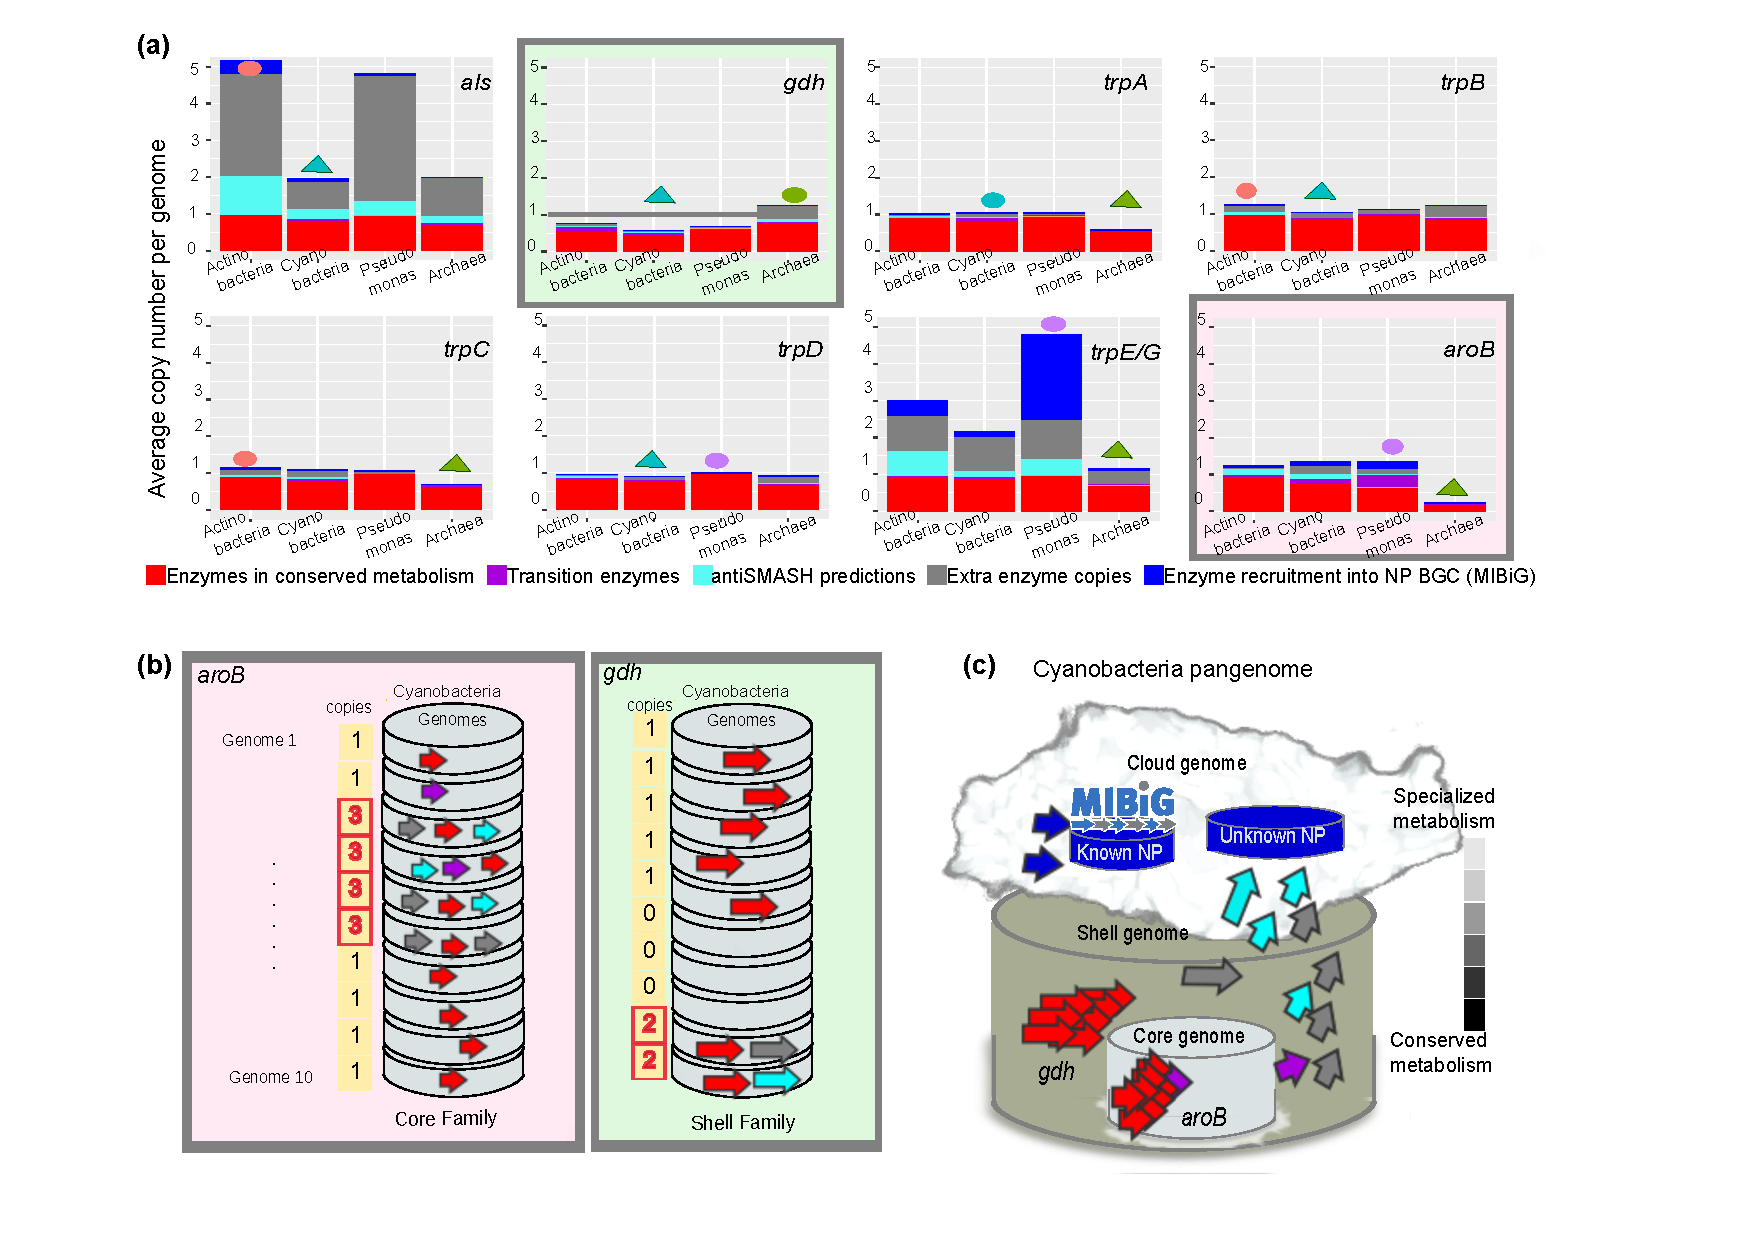
\includegraphics[angle = 0,scale = .6]{chapter2/FigurasPaper/Figure3.pdf}
  \caption[Expansion patterns in 42 conserved families]{\footnotesize{EvoMining perfiles de enzimas conservadas seleccionadas. (a) Patrones de expansión de las ocho familias conservadas cuyas copias adicionales participan en la biosíntesis de scytonemin. El conjunto completo de 42 EF se muestra en la Fig. S11. La codificación de colores es la siguiente: rojo para el metabolismo conservado, azul para los reclutamientos anotados en MIBiG, cian para las predicciones antiSMASH de metabolismo especializado, púrpura para la intersección entre el metabolismo conservado y las predicciones antiSMASH, y gris para las expansiones sin destino metabólico conocido. El orden en el eje x es Actinobacteria, Cianobacteria, Pseudomonas y Archaea. Los triángulos indican el linaje con el mayor número de copias por genoma en promedio, y los círculos representan el linaje menos expandido. Aunque Archaea tiende a ser los taxones menos expandidos, esta tendencia se revierte en la familia GDH. (b) Se proporciona un ejemplo de un núcleo frente a un shell EF. AroB es un EF básico porque tiene al menos una copia por genoma, mientras que GDH es un EF de shell debido a su ausencia en tres genomas. A pesar de ser un shell EF, GDH tiene copias adicionales que pueden ser reclutadas en un metabolismo especializado. (c) Modelo para la $nube$ o genoma variable compuesto parcialmente por enzimas que pertenecen a BGC NP. En este modelo, el metabolismo conservado se compone de EF tanto de shell como de núcleo. Estos EF pueden sufrir eventos de expansión, y algunas de las copias adicionales son reclutadas para realizar nuevas funciones en el metabolismo especializado.}}
  \label{fig:ExpansionPatterns}
  \end{figure}
  
  Todos los linajes tienen patrones de expansión similares en las 42 FEs
  analizadas hasta un tamaño de genoma 5 Mbp. En genomas más grandes, el
  número total de secuencias crece más en Pseudomonas que en el phylum
  Actinobacteria, que es más grande que el phylum Cyanobacteria y que el
  dominio Archaea \autoref{fig:SeedGenomes} panel(b). Este resultado puede
  deberse a que no se han descubierto tamaños de genoma Archaea de tamaño
  comparable a los de Streptomyces o Pseudomonas (\(> 5\)Mbp).
  Cyanobacteria a pesar de tener genomas grandes no tiene tantas
  expansiones. Esta observación, es posible que sea generalizable a todas
  las EFs de metabolismo conservado o bien que se deba a un sesgo en la
  selección de las familias que componen a la EFs.
  
  Los órdenes con mayor número de copias fueron en las expansiones de las
  familias de la Enzyme DB fueron Streptomycetales y Nostocales , en
  Actinobacteria y Cyanobacteria respectivamente. Esta observación es
  congruente con que estos órdenes tienen un tamaño de genoma grande en
  sus linajes correspondientes, y además están ampliamente representados
  en MIBiG como sintetizadores de productos naturales. Interesantemente la
  clase Halobacteria es la que muestra mayor número de expansiones en
  Archaea, aunque no es la clase con mayor tamaño de genoma en promedio
  (Fig. S10). {[}FIGURA tamaño de genoma{]}
  
  Esta observación es congruente con que las archaeocinas,
  dicetopiperazinas, carotenoides y otros productos naturales de Archaea
  fueron aislados de especies de Halobacteria, los NP BGCs sintetizadores
  de estos metabolitos no han sido caracterizados
  {[}\protect\hyperlink{ref-charlesworth_untapped_natural_products_Archaea_2015}{154}{]}.
  Por ello EvoMining una herramienta de minería genómica que puede ayudar
  a explorar linajes poco minados con el potencial de descubrir nuevas
  rutas metabólicas.
  
  La figura muestra que aunque en las familias conservadas seleccionadas
  el número de copias extra correlaciona con el tamaño de genoma los
  perfiles de expansiones son diferentes en cada grupo taxonómico. Este
  incremento parece cambiar su patrón en todos los linajes a partir de
  5Mbp \autoref{fig:SeedGenomes} (2b). Acorde a estos resultados se
  concluye que para ensamblar una base de datos genómica para EvoMining se
  debe considerar que las expansiones dependen tanto de los distintos
  linajes taxonómicos como de la diversidad del tamaño de genoma.
  
  \subsection{El shell genome posee expansiones en sus familias
  enzimáticas}\label{el-shell-genome-posee-expansiones-en-sus-familias-enzimaticas}
  
  La figura muestra que Pseudomonas posee en promedio más copias por
  genoma que los otros taxa. De las 42 familias analizadas el \(54.8\%\)
  tiene su máximo número promedio de copias por genoma en este linaje.
  (Fig. S11). En contraste, Actinobacteria es el máximo en \(26.2\%\) de
  las FEs, mientras que Archaea and Cyanobacteria empatan en ser el linaje
  con más expansiones sólo en el \(9.5\%\) de los casos (Table S1). Aunque
  existen familias como la acetylornitino aminotransferasa o la
  acetolactato sintasa (ALS) que están expandidas en todos los linajes
  (coordenadas A1 y E1, Fig. S11), muchas otras familias exhiben
  expansiones sólo en ciertos linajes. Tal es el caso de la fumarato
  reductasa subunidad de hierro-azufre (coordinate C3, Fig. S11), muy
  expandida en Actinobacteria pero con menos de una copia por genoma en
  promedio en Cyanobacteria .
  
  No todas las FEs están expandidas, aunque las 42 familias conservadas
  están presentes en alguno de los genomas semilla de cada linaje, varias
  de ellas no se encuentran en la mayoría de los genomas del resto de su
  base de datos. Este es el caso de AroB en Archaea, donde tiene muy poca
  representación. Sin embargo, un gran porcentaje de familias muestra
  perfiles de expansión acordes a la tendencia del número total de copias
  extra, mostrada en la figura XX. Es decir, por familia Pseudomonas suele
  ser el linaje con el mayor número de expansiones mientras que Archaea
  suele ser el linaje menos expandido. Entre las excepciones a esta
  tendencia está GDH una familia incluida dentro de los ocho casos
  seleccionados para ilustrar esta diversidad que son mostrados en la
  figura \autoref{fig:ExpansionPatterns}\\
  panel (a). En esta figura los máximos están marcados con un círculo
  mientras que los mínimos con un triángulo, los colores de estas formas
  geométricas representan los mismos linajes que los mostrados en la
  \autoref{fig:SeedGenomes}. Del total de las 42 familias, GDH es una de
  las cuatro FEs en las que el mayor número de expansiones se encuentra en
  Archaea. De hecho, GDH tiene menos de una copia por genoma en promedio
  en los otros taxa, probando que no se encuentra dentro del core genómico
  de estos linajes. Esto contrasta con AroB, que muestra una tendencia
  opuesta, no es parte del core de Archaea pero muestra copias extra y una
  presencia mayor que uno en promedio en los otros tres taxa analizados
  \autoref{fig:ExpansionPatterns} panel (b). Los ocho casos mostrados en
  la figura son todos parte de un cluster biosintético de Cyanobacteria,
  descrito en las secciones posteriores de este trabajo.
  
  \begin{figure}[h!tbp]
  \centering
  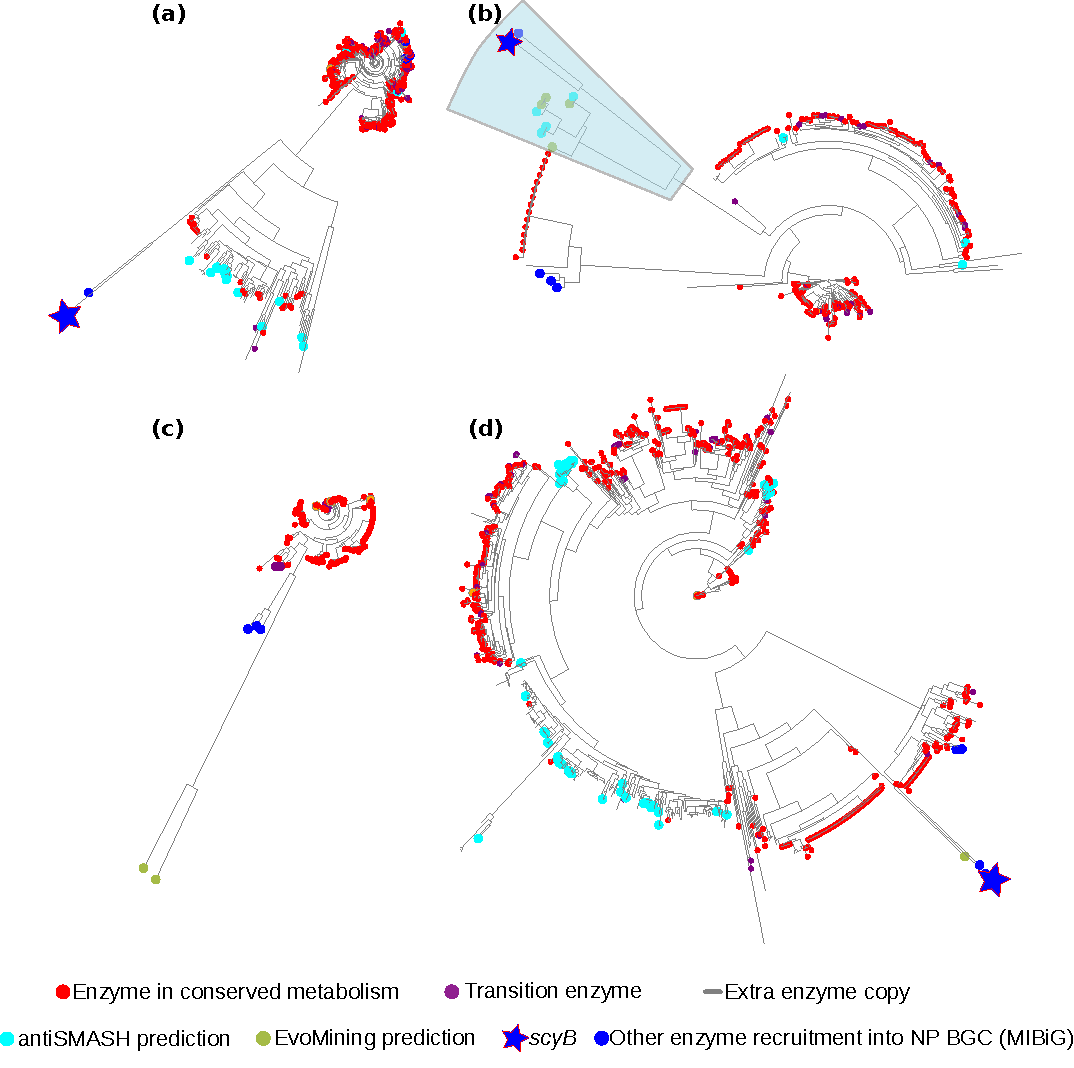
\includegraphics[angle = 0,scale = .8]{chapter2/FigurasPaper/Figure4.pdf}
  \caption[EvoMining en cuatro linajes genómicos]{\footnotesize{n}}
  \label{fig:GenomicLinajes}
  \end{figure}
  
  Con estas observaciones sospechamos que GDH es miembro del shell genome
  {[}\protect\hyperlink{ref-koonin_genomics_2008}{155}{]} en los taxa
  Actinobacteria , Cyanobacteria y Pseudomonas, ya que en promedio está
  cerca de tener una copia promedio por genoma. El promedio no es
  suficiente para decir que una familia pertenece al shell, podrían
  suceder casos sobre todo cuando hay mucha variación n un taxon como en
  el caso de un domino o un phylum en contraposición con taxones
  coservados como géneros en los que para una cierta familia la mitad de
  los genomas de un linaje tuviera dos copias y la otra mitad cero. Sin
  embargo en el caso de la GDH si es consistente en que está presente en
  más del \(50\%\) de los genomas de cada linaje
  \autoref{fig:ExpansionPatterns} panel (a). Las modas de número de copias
  también son informativas por ello son mostradas en la figura XXX. Una
  sóla copia extra puede ser la que sea reclutada en metabolismo
  especializado.
  
  En la figura XXX se muestra un ejemplo donde AroB es una enzima core en
  oposición a GDH que es una enzima shell. En este esquema conceptual, en
  algunos de los genomas que contienen a AroB existen copias que se
  dedican al metabolismo especializado marcadas en color cyan, otras
  copias no tienen un destino metabólico conocido por lo que están
  marcadas en gris, y otras más marcadas en púrpura son enzimas de
  transición que están llevando a cabo simultáneamente una función en
  metabolismo central y otra en metabolismo especializado. En contraste a
  AroB se muestra GDH, que a pesar de no tener copias en algunos genomas y
  con un promedio de copias por genoma menor a uno y una moda de uno en
  esta muestra, GDH existe por duplicado en dos genomas. En uno de esos
  genomas donde GDH tiene una copia extra, más allá de la moda, esa copia
  se muestra como un reclutamiento al metabolismo especializado en cyan.
  \autoref{fig:ExpansionPatterns} panel (b) .
  
  Las expansiones encontradas por EvoMining en la familia GDH incluían
  predicciones de antiSMASH para Actinobacteria, Cyanobacteria y Archaea,
  no así para Pseudomonas. La secuencia del reclutamiento de GDH por los
  clusters biosintéticos scytonemin y el policétido pactamycin
  {[}\protect\hyperlink{ref-kudo_cloning_2007}{156}{]}, es suficientemente
  parecida como para que EvoMining la detecte como expansión en
  Actinobacteria, Cyanobacteria y Archaea, pero es tan divergente respecto
  a la familia GDH en Pseudomonas que EvoMining lo deja fuera de la
  familia expandida en este linaje. Los árboles donde puede apreciarse
  esta observación pueden consultarse más adelante en la
  \autoref{fig:GenomicLinajes} de la siguiente sección.
  
  Los resultados anteriores sugieren que la evolución del metabolismo
  especializado es linaje dependiente, y más aún que tal y como ya se
  conocía en las FEs del core genome las enzimas del shell como GDH
  también poseen el potencial de ser reclutadas en NP BGCs. A partir de
  estos resultados \autoref{fig:ExpansionPatterns} paneles (a,b), se
  realizó un esquema conceptual para explicar cómo en linajes genómicos
  diversos las familias de enzimas con origen en el metabolismo central
  que forman parte del core genome o bien las familias en el metabolismo
  conservado que incluye tanto al core como al shell genome, evolucionan
  al metabolismo especializado que tiene una mayor representación en el
  cloud genome \autoref{fig:ExpansionPatterns} panel (c) . Este modelo es
  relevante porque establece el papel de las familias del shell genome,
  que no fue considerado en la primera iteración que explotó las
  capacidades de EvoMining como herramienta de minería genómica para
  encontrar BGCs
  novedosos{[}\protect\hyperlink{ref-navarro-munoz_computational_2018}{157}{]}.
  
  \begin{figure}[h!tbp]
  \centering
  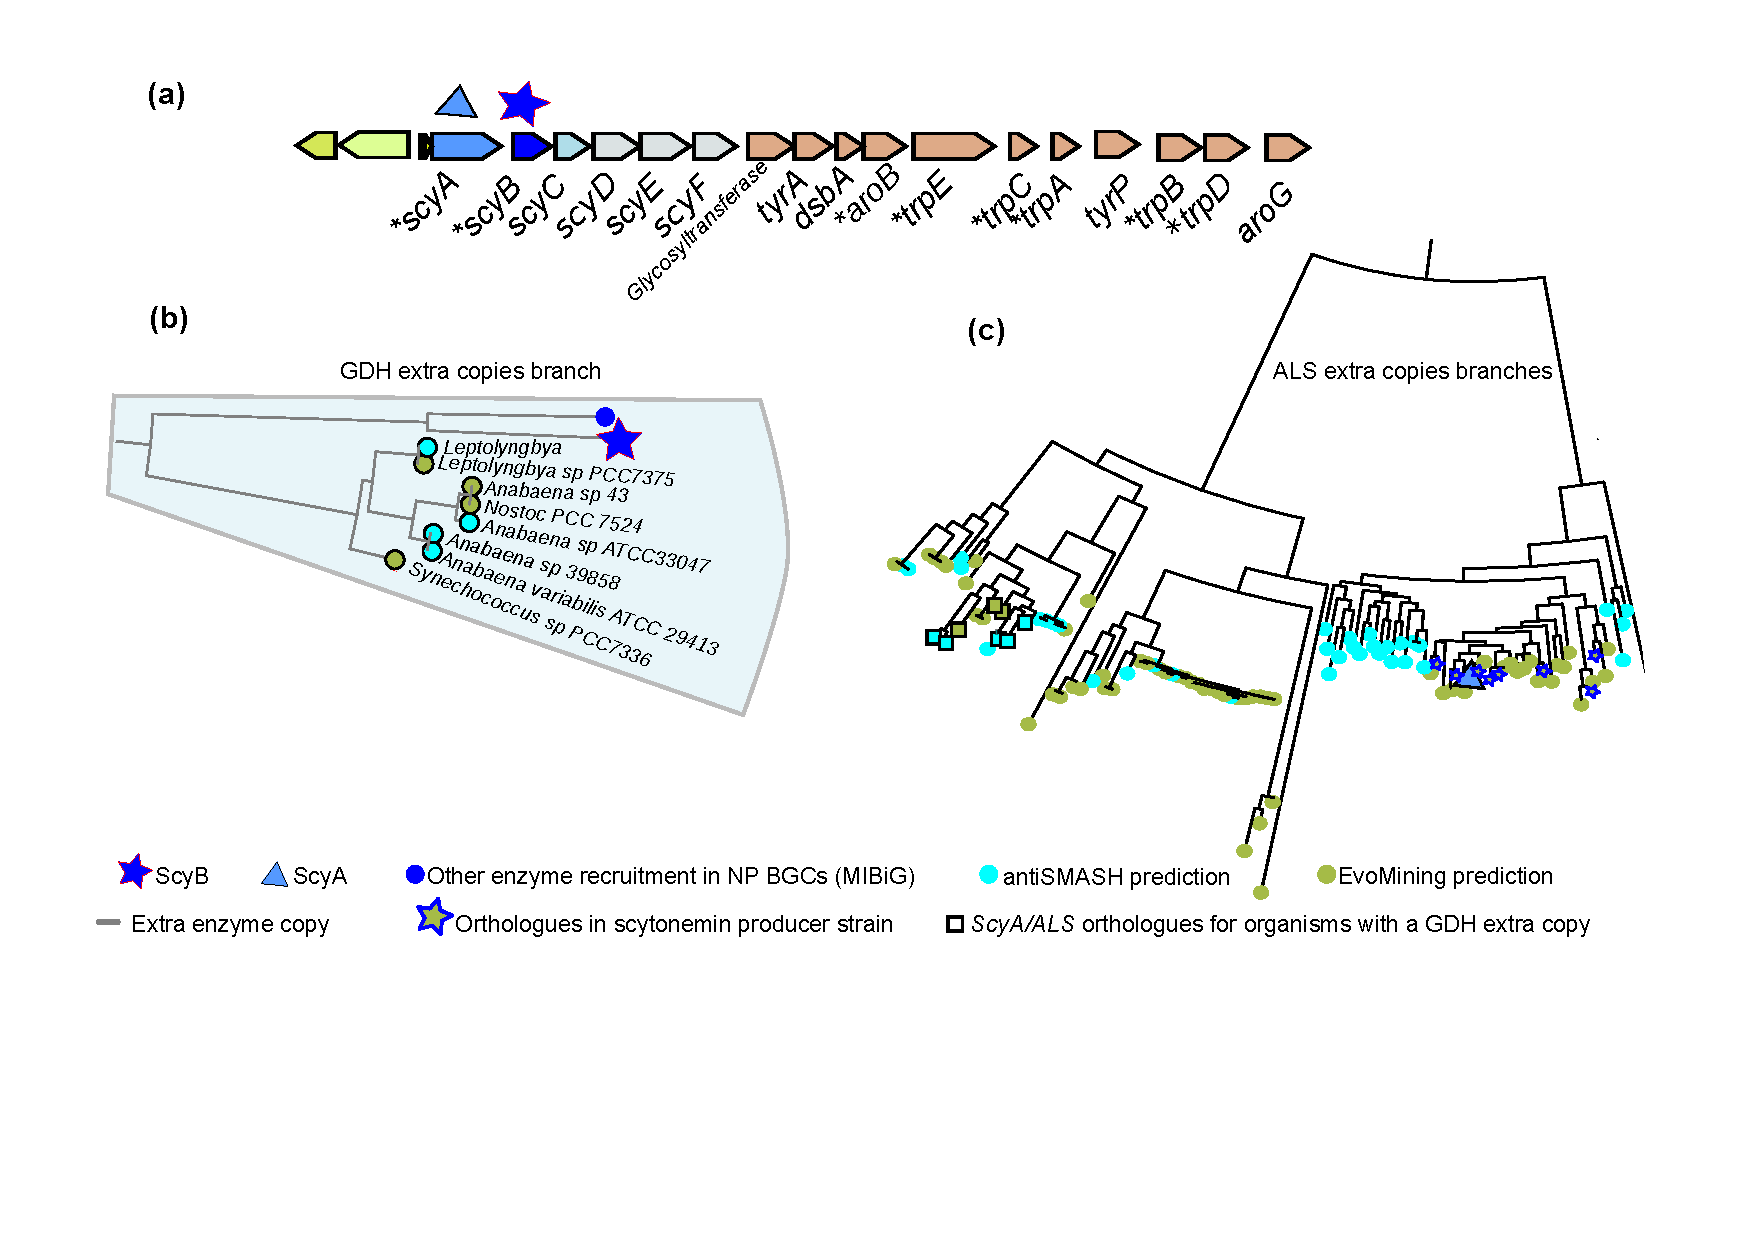
\includegraphics[angle = 0,scale = .6]{chapter2/FigurasPaper/Figure5.pdf}
  \caption[EvoMining aplicado a la rama de scytonemina]{\footnotesize{}}
  \label{fig:Scytonemin}
  \end{figure}
  
  En la siguiente sección se analizarán los patrones de expansión
  reclutamiento de GDH provistas por EvoMining for GDH y se describirán
  los árboles filogenéticos de cada linaje mostrados en la
  \autoref{fig:GenomicLinajes} , así como un árbol que incluye
  conjuntamente secuencias de todos los linajes (Figs S12 and S13). En
  Archaea, GDH tiene en promedio 1.23 copias por genoma, mientras en
  Actinobacteria, Cyanobacteria y Pseudomonas esta media es de 0.74, 0.56
  y 0.65, respectivamente. En estos tres taxa GDH es parte del shell
  genome (Table S2).
  
  Además de GDH se estudiaron las expansiones y los árboles filogenéticos
  de TrpA, TrpB, TrpC, TrpD, TrpEG, AroB y ALS, todas ellas parte de las
  42 FEs conservadas entre los cuatro linajes y a la vez reclutadas en
  scytonemin{[}\protect\hyperlink{ref-balskus_investigating_2008}{143}{]}
  un cluster biosintético de Cyanobacteria
  
  \subsection{GDH y ALS en el cluster scytonemin ejemplifican como
  familias pertenecientes a un mismo BGC pueden tener distintos patrones
  de
  expansión.}\label{gdh-y-als-en-el-cluster-scytonemin-ejemplifican-como-familias-pertenecientes-a-un-mismo-bgc-pueden-tener-distintos-patrones-de-expansion.}
  
  La enzima GDH, se encuentra presente en muchos linajes debido tanto a su
  origen ancestral como a la transferencia horizontal {[} 28, 42 {]} (Fig.
  S12). GDH cataliza la reacción reversible de desaminación oxidativa de
  glutamato en \(\alpha\)-cetoglutarato y amonio. De acuerdo al uso de
  cofactores GDH puede dividirse en tres clases, la primera usa NAD+ y es
  nombrada como GDH(NAD+). La segunda clase utiliza NADP+ y es conocida
  como GDH(NADP+). La tercera clase utiliza ambos cofactores NAD+ y NADP+;
  por lo que se le conoce como GDH(NAD+ y
  NADP+){[}\protect\hyperlink{ref-engel_glutamate_2014}{145}{]}.
  
  Aunque existen otras clasificaciones de la diversidad de enzimas GDH
  esta fue seleccionada porque se relaciona con la historia evolutiva de
  la enzima. GDH(NAD+) is utilizada para la oxidación del glutamato
  mientras que GDH(NADP+) para fijar amonio, algunas enzimas de Archaea
  funcionan bien con ambos cofactores, es decir tienen promiscuidad de
  cofactores{[}\protect\hyperlink{ref-engel_glutamate_2014}{145}{]}. La
  especificidad por NAD o NADP probablemente emergió en repetidas
  ocasiones, una evidencia a favor de esta hipótesis es que se ha mostrado
  que algunas mutaciones pueden revertir la
  especificidad{[}\protect\hyperlink{ref-lilley_partial_1991}{158}{]}.
  Esto sugiere que en los cofactores análogamente al caso de promiscuidad
  por sustrato, la similitud de secuencia no siempre es suficiente para
  evidenciar la especificidad. En ocasiones la divergencia o cercanía
  filogenética de los organismos productores de la enzima es una
  información adicional a la similitud de secuencia, esta consideración es
  importante al analizar enzimas en linajes muy divergentes.
  
  La familia GDH muestra expansiones aunque no muy abundantes en
  \href{https://microreact.org/project/r1IhjVm6X?tt=cr}{Actinobacteria}
  \autoref{fig:GenomicLinajes} panel (a) ,y en
  \href{https://microreact.org/project/HyjYUN7pQ?tt=cr}{Cyanobacteria}
  \autoref{fig:GenomicLinajes} panel(b). Las expansiones están
  prácticamente ausentes en
  \href{https://microreact.org/project/HyjYUN7pQ?tt=cr}{\emph{Pseudomonas}}
  \autoref{fig:GenomicLinajes} panel (c). En contraste, un número
  significativo de expansiones es encontrado en
  \href{https://microreact.org/project/ByUcvNmaX?tt=cr}{Archaea}
  \autoref{fig:GenomicLinajes} panel(d) . El árbol de EvoMining de la
  familia GDH en Archaea fue enraizado con la secuencia semilla de
  \emph{Sulfolobus}, que fue predicha por RAST como una enzima dual en el
  uso de cofactores
  NAD(P)+{[}\protect\hyperlink{ref-consalvi_glutamate_1991}{159}{]}. En
  Archaea las tres clases de GDH alternan en las ramas del
  \href{https://microreact.org/project/ByUcvNmaX?tt=cr}{árbol} (Fig.
  S13,).
  
  Muchas de las secuencias clasificadas como de metabolismo conservado se
  concentran volviendo rojas las ramas basales del árbol. Se observa otro
  clado más grande y diverso compuesto casi exclusivamente por enzimas
  específicas para
  NAD(P){[}\protect\hyperlink{ref-ferrer_nadp-glutamate_1996}{160}{]},
  incluyendo muchas predicciones de antiSMASH, y sólo dos marcadas como
  metabolsimo conservado. Estas dos marcas pueden deberse a la pérdida
  real de una enzima d metabolismo central en las ramas centrales o bien a
  huecos debidos a la calidad del ensamblado y la secuenciación de los
  genomas.
  
  La anotación funcional de estos ortólogos de GDH apunta hacia
  reclutamientos en el metabolismo especializado. Estos reclutamientos
  fueron identificados en organismos de los genera \emph{Haladaptatus},
  \emph{Haloterrigena} , \emph{Natrialba} , \emph{Natrinema} ,
  \emph{Natrialbaceae} y \emph{Natronococcus}. Los genes codificante se
  encuentran un contexto de posible síntesis de terpenos. Este contexto
  incluye enzimas relacionadas al geranyl pyrofosfato, un precursor de
  todos los terpenos y
  terpenoides{[}\protect\hyperlink{ref-tholl_terpene_2006}{161}{]}. Este
  árbol tiene también casos de divergencia reciente, hay una pequeña rama
  indistinguible en la figura pero explorable en la plataforma microreact
  donde los parálogos aparecen junto a las secuencias de metabolismo
  central. Finalmente a pesar de la divergencia las últimas ramas
  corresponden a enzimas de metabolismo conservado, es decir son las
  copias más parecidas en esos organismos a las semillas provistas en la
  Enzyme DB \autoref{fig:GenomicLinajes} panel(d).
  
  En contraste con la amplia expansión de GDH relacionada a las
  adaptaciones metabólicas en Archaea, el árbol de Cyanobacteria tiene
  copias extra sólo en el \(4.5\%\) de sus genomas (
  \autoref{fig:GenomicLinajes} panel(b) , Table S2). En esta rama
  expandida se encontraron cuatro predicciones de antiSMASH y cuatro
  predicciones de EvoMining en la rama que contiene a ScyB el homólogo de
  GDH que fue reclutado por el BGC scytonemin. ScyB es pues parte de la
  síntesis de scytonemin, un pigmento amarillo producido por muchas
  Cyanobacterias como protección contra la radiación UV-A
  solar{[}\protect\hyperlink{ref-balskus_genetic_2010}{162}{]}.
  \emph{Nostoc punctiforme} PCC 73102 es el organismo productor de
  scytonemin cuyo BGC fue caracterizado y anotado en MIBiG. EvoMining sólo
  unas pocas secuencias GDH copias extra de especies de Nostoc aún cuando
  se conoce que homólogos de scyB pueden encontrarse en estos genomas.
  Esta observación puede deberse a la gran divergencia de secuencia entre
  copias de metabolismo central y de metabolismo especializado en estos
  organismos.
  
  En la vecindad genómica de algunas expansiones de GDH se observó la
  secuencia de ALS, un gen identificado en la literatura como homólogo de
  \emph{scyA}. además, en los BGC conocidos de scytonemin se observó que
  \emph{scyB} se conserva cerca del gene \emph{scyA}
  \autoref{fig:Scytonemin} panel (a). \emph{scyA} es homólogo de la
  subunidad larga de ALS. Esta familia tiene un número promedio de copias
  de \(1.87\%\) en la base de datos Genome DB de Cyanobacteria. La media
  es de hecho de \(2.1\) copias en organismos que contienen al menos una
  copia ALS, pero la moda del número de copias es 1 (Table S2). Estos
  datos indican que muchos organismos tienen más de dos copias de ALS lo
  que puede correlacionar con que esta familia es más dispersa alrededor
  de la moda (Fig. S4, blue line).
  
  Al generar el
  \href{https://microreact.org/project/B11HkUtdm?tt=cr.}{árbol de
  EvoMining de ALS en Cyanobacteria} , Fig. S11, se observó que
  \emph{scyA} es un reclutamiento que se localiza en una rama repleta de
  secuencias de ALS provenientes de \emph{Nostoc spp.}, que fueron
  etiquetadas como predicciones de EvoMining \autoref{fig:Scytonemin} (c).
  Estas predicciones incluyen más de veinte organismos conocidos como
  productores de scytonemin
  {[}\protect\hyperlink{ref-balskus_investigating_2008}{143}{]}
  
  Además, ramas cercanas muestran secuencias de ALS queson p redicciones
  de antiSMASH, reforzando la sugerencia de que esta seción del árbol se
  dedica al metabolismo especializado. Una última rama contiene a los
  mismos organismos encontrados en el árbol de EvoMining de la familia
  GDH. Estos organismos son mostrados en el zoom de la rama de \emph{scyB}
  \autoref{fig:Scytonemin} panel(b).
  
  \begin{figure}[h!tbp]
  \centering
  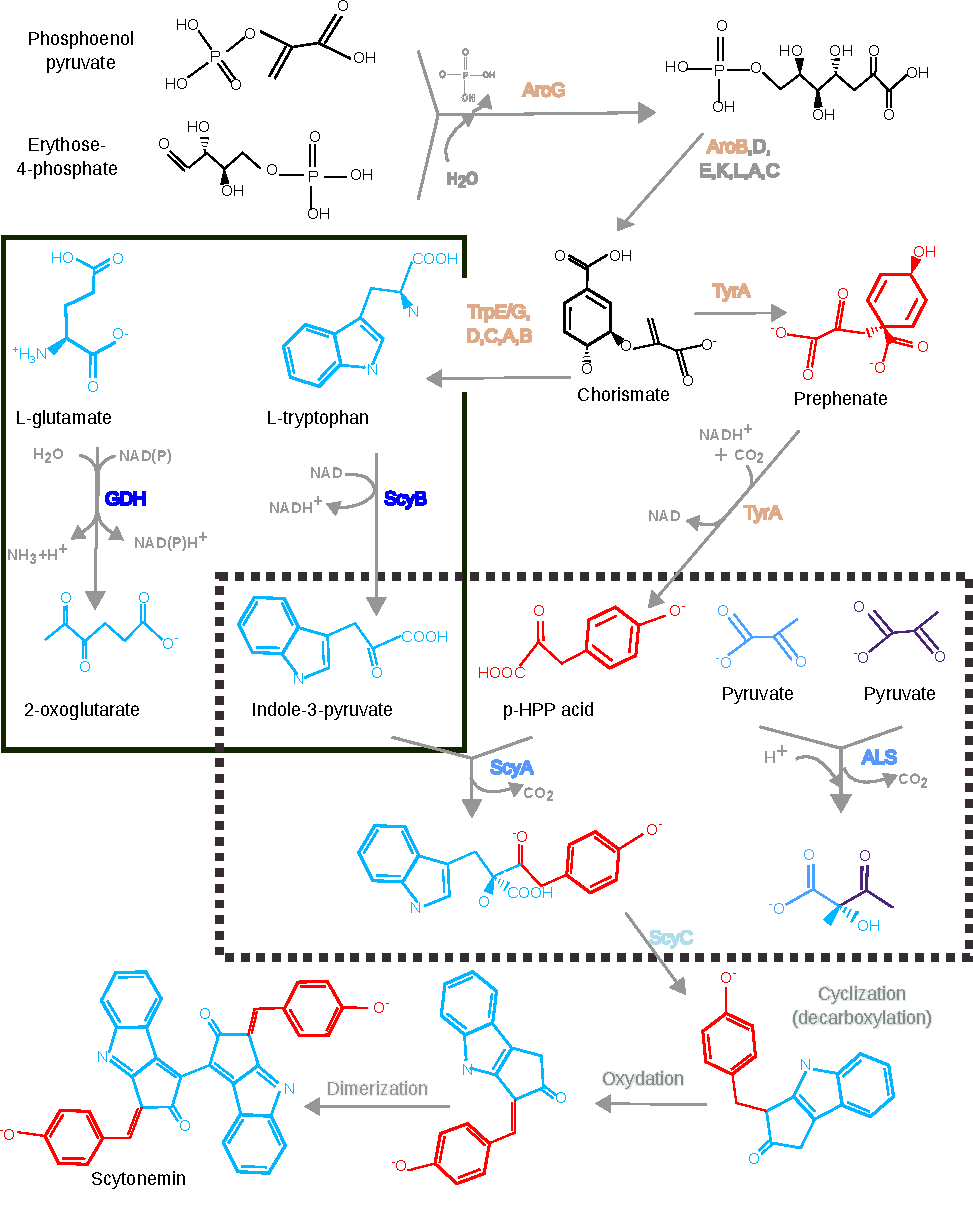
\includegraphics[angle = 0,scale = .8]{chapter2/FigurasPaper/Figure6.pdf}
  \caption[EvoMining Algorithm]{\footnotesize{}}
  \label{fig:Ruta}
  \end{figure}
  
  Esta observación sugiere co-diversificación, vía un evento de expansión
  reclutamiento de ScyA y ScyB a partir de su origen en ALS y GDH,
  respectivamente. Los perfiles de expansin de estas familias difieren ya
  que a diferencia de la muy poblada rama de \emph{scyA} en el árbol de
  ALS, la similitud entre homólogos de GDH EF y homólogos de ScyB no fue
  suficiente para reconstruir una rama de \emph{scyB} con todas las
  expansiones sugeridas por la ocurrencia del cluster de scytonemin. Estas
  observaciones son una lección a usar EvoMining como herramienta de
  minería genómica, que enzimas cercanas pueden co-diversificarse en
  ocasiones formando parte de un mismo BGC pero a la vez estar sujetas a
  distintas restricciones evolutivas.
  
  \subsection{El cluster de scytonemin es un cluster
  promiscuo.}\label{el-cluster-de-scytonemin-es-un-cluster-promiscuo.}
  
  El primer cluster caracterizado de scytonemin, mostrado en la figura
  \autoref{fig:Scytonemin} panel (a) y en \autoref{fig:Ruta} , comprende
  18 genes {[}\protect\hyperlink{ref-soule_comparative_2009}{144}{]}.
  Además de genes reguladores, este BGC incluye genes biosintéticos
  scyABC; otros genes conservados cuya función queda por dilucidar,
  scyDEF; y proveedores de precursores: \emph{tyrA}, \emph{dsbA},
  \emph{aroB}, \emph{trpE/G}, \emph{trpC}, \emph{trpA}, \emph{tyrP},
  \emph{trpB}, \emph{trpD}, \emph{aroG}. Las familias enzimáticas
  TrpABCDEG y AroB son parte de las rutas de los aminoácidos aromáticos y
  el ácido shikímico, parecen haber sido reclutadas para proveer de los
  precursores L-triptofano y prefrenato necesarios para la síntesis de
  scytonemin. En oposición a los genes del operon \emph{trp} y a AroB que
  siguen realizando su función de metabolismo conservado aún al ser parte
  de una ruta de metabolismo especializado están ScyA y ScyB. Estas dos
  familias también tienen un origen en el metabolismo conservado, ya se ha
  explicado que tienen su origen en las familias ALS y GDH, pero en este
  caso sí ha cambiado la especificidad por sustrato al momento de la
  incorporación al metabolismo especializado \autoref{fig:Ruta}. ALS une
  dos piruvatos, transformándolos en S-2-acetolactato
  {[}\protect\hyperlink{ref-liu_acetohydroxyacid_2016}{146}{]}, mientras
  que ScyB cataliza la unión de indol-3-piruvato con p-hydroxy-fenil-ácido
  pirúvico. Análogamente GDH convierte L-glutamate en 2-oxoglutarato
  {[}\protect\hyperlink{ref-engel_glutamate_2014}{145}{]}, mientras que
  ScyA cataliza una desaminación oxidativa de triptofano. El producto de
  estas dos enzimas actuando secuencialmente e un dipéptido, el cual es
  ciclizado por ScyC. La ruta metabólica culmina con una serie de
  oxidaciones y dimerizaciones hasta llegar al producto scytonemin, aún no
  es claro como estos útimos pasos se llevan a cabo
  {[}\protect\hyperlink{ref-balskus_investigating_2008}{143}{]}.
  
  \begin{figure}[h!tbp]
  \centering
  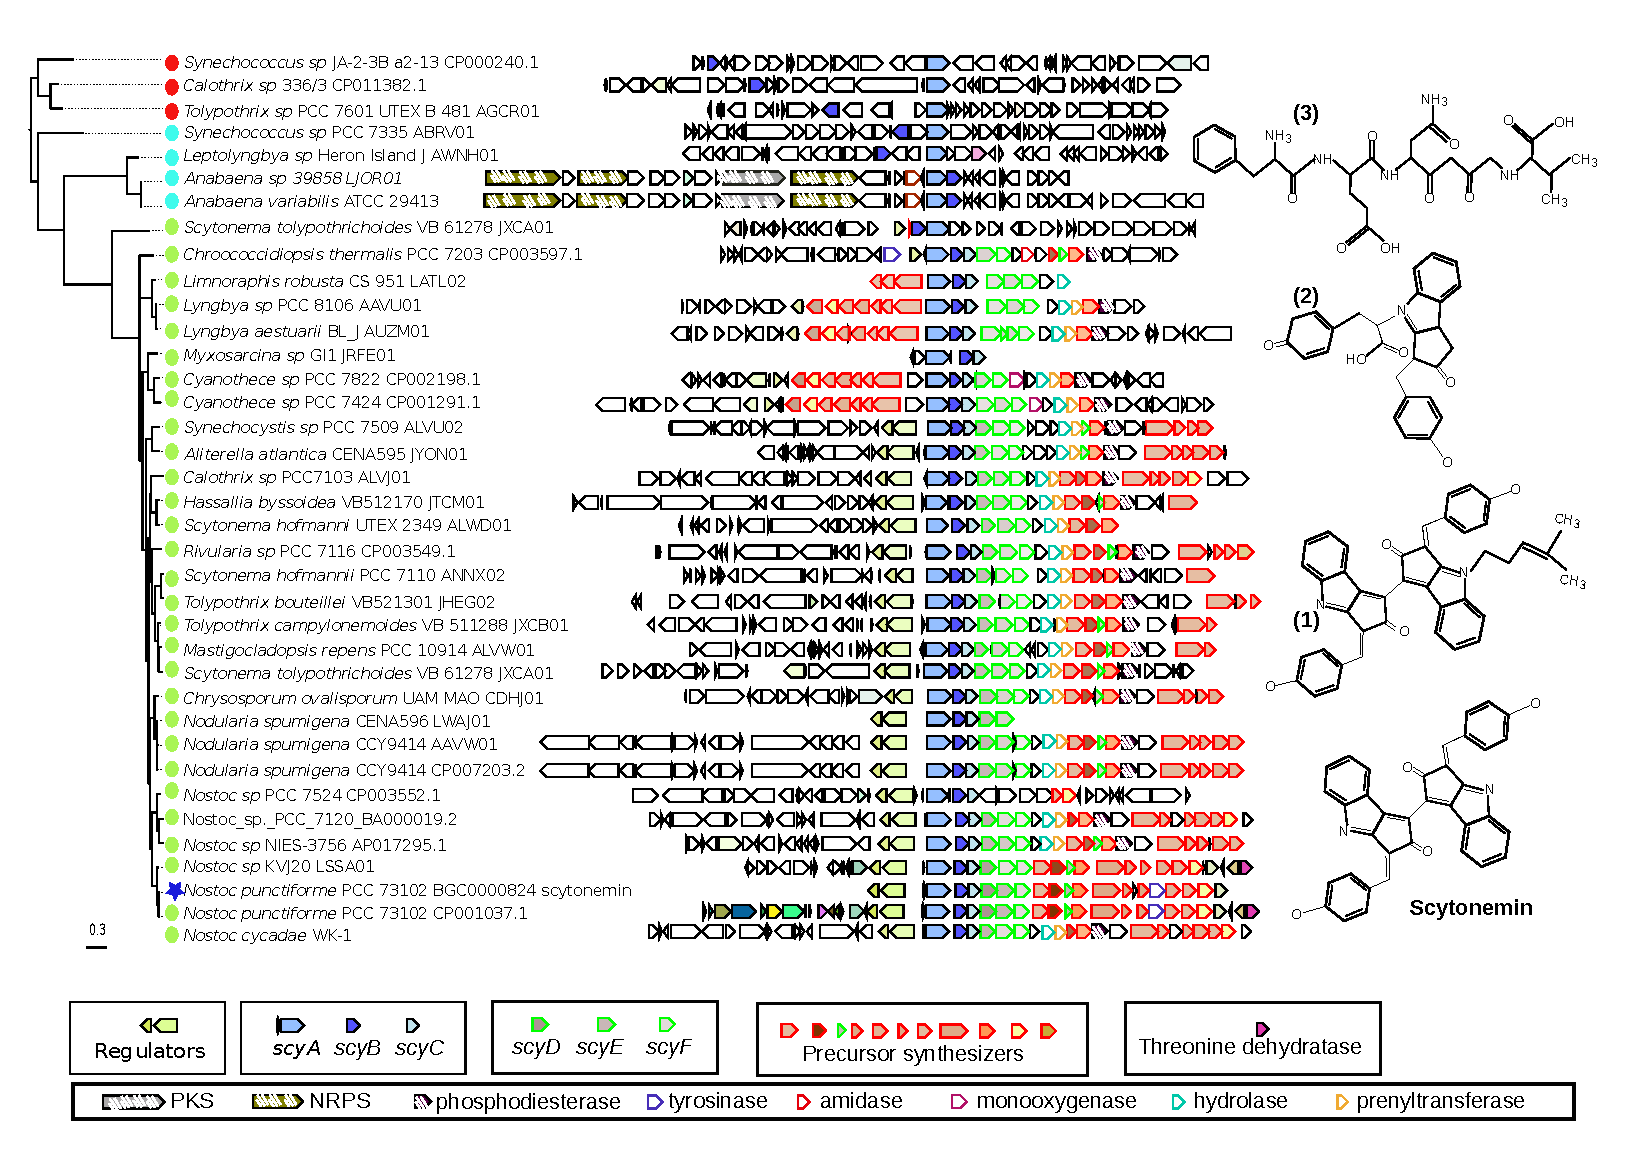
\includegraphics[angle = 90,scale = .8]{chapter2/FigurasPaper/Figure7.pdf}
  \caption[EvoMining Algorithm]{\footnotesize{}}
  \label{fig:CorasonScytonemina}
  \end{figure}
  
  Además de GDH y ALS el BGC de scytonemin tiene seis familias que son
  parte de las 42 FEs analizadas aquí, es decir 8 de los genes que
  participan en la síntesis de scytonemin tienen un origen en metabolismo
  central y fueron reclutados en el cluster de scytonemin (
  \autoref{fig:ExpansionPatterns} panel 1, Table S3). (
  \autoref{fig:Scytonemin} and S3--S9). De estas familias, seis de los
  siete árboles de EvoMining contienen copias extras identificadas como
  predicciones de EvoMining predictions, debido a que en su rama de
  expansión se encuentra el correspondiente gen de scytonemin del cluster
  reportado en MIBiG. Estas familias incluyen AroB y todos los genes de la
  ruta del L-triptofano excepto trpF. Además los árboles de EvoMining de
  estas familias incluyen predicciones en ramas que con enzimas
  provenientes de las rutas de síntesis de otros pigmentos protectores
  solares como la shinorina y los aminoácidos de tipo mycosporina
  \autoref{fig:AroB}
  {[}\protect\hyperlink{ref-balskus_genetic_2010}{162}{]} , además de
  otros productos no relacionados como la welwitindolinona
  {[}\protect\hyperlink{ref-hillwig_identification_2014}{163}{]},
  ambiguina
  {[}\protect\hyperlink{ref-li_hapalindole_ambiguine_2015}{164}{]} y la
  fischerindolina {[}\protect\hyperlink{ref-li_decoding_2017}{165}{]}
  (Figs S3--S7). Estos resultados ilustran como EvoMining puede
  complementar a antiSMASH mediante la identificación de secuencias de NP
  BGCs no tradicionales.
  
  \begin{figure}[h!tbp]
  \centering
  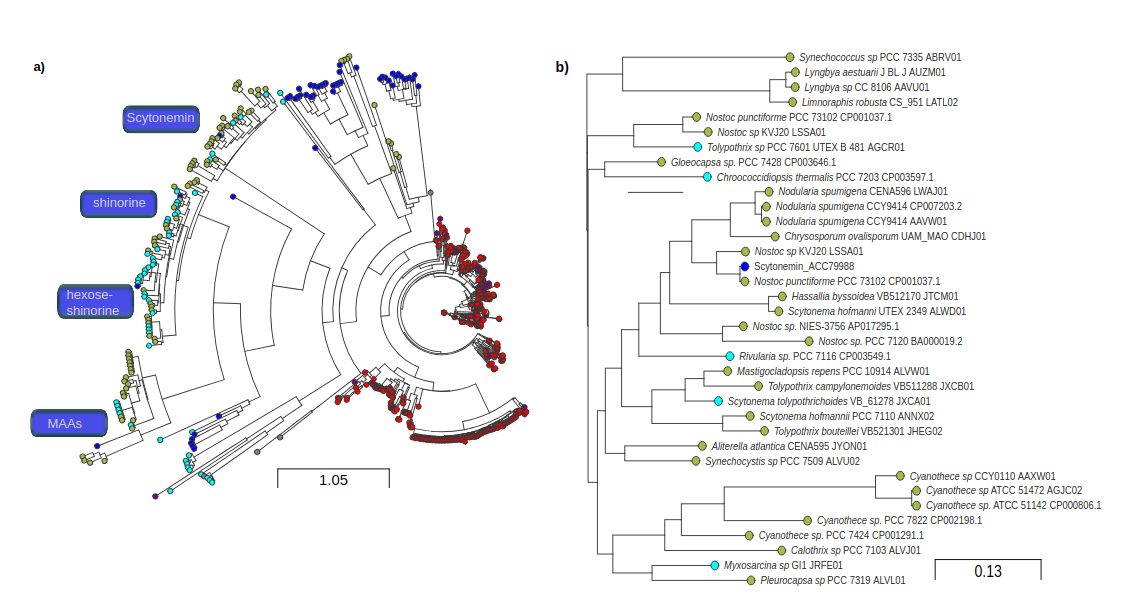
\includegraphics[angle = 0,scale = .48]{EvoMining/supplementary/AroB.png}
  \caption[AroB en Cyanobacteria]{\footnotesize{}}
  \label{fig:AroB}
  \end{figure}
  
  Para investigar la coocurrencia de ScyA y ScyB, que son necesarias
  juntas para producir scytonemin, reconstruimos su historia evolutiva
  conjunta. Para ello se obtuvieron las secuencias de lo genomas donde
  ambas tenían presencia, se concatenaron sus secuencias y se realizó una
  filogenia con ellas. Las variantes de la vecindad genómica del BGC de
  scytonemin fueron visualizadas mediante el uso de corason
  {[}\protect\hyperlink{ref-navarro-munoz_computational_2018}{157}{]}. En
  el siguiente capítulo este software de visualización y organización de
  vecindades genómicas será explicado con más detalle. Los análisis
  filogenómicos resultaron en 34 cyanobacterias con diversidad química en
  el BGC de scytonemin. Es decir en concusión scytonemin es un ejemplo de
  cluster promiscuo, ya que parece haber un core conservado, pero
  diversidad en enzimas accesorias y por tanto en sus productos finales.
  
  Se pudieron predecir cinco estructuras putativas que son variantes de
  scytonemin y correlacionan con episodios de pérdida y ganancia de genes
  en este locus \autoref{fig:CorasonScytonemina}. Al core de genes scyABCD
  se incorporan genes que realizan ornamentos como hidrolasas,
  prenil-transferasas , fosfodiesterasas y monooxigenasas , para formar
  congéneres de scytonemin como los compuestos 1 y 2. La pérdida de los
  genes \emph{scyDEF} y la aparición de otras enzimas como la tyrosinase y
  o la amidasa pueden derivar en la síntesis de los compuestos 3 and 4.
  Además encontramos que homólogos de scyA y scyB son parte de otro BGC
  que contiene un híbrido NRPS-PKS. Siguiendo las reglas biosintéticas de
  estas enzimas se propuso el compuesto 5. La diversidad química sugerida
  en estas predicciones sólo puede ser validado mediante el trabajo
  experimental. Las variantes producidas por la dinámica evolutiva del
  metabolismo especializado fueron sugeridas mediante el sólo uso de ScyA
  y ScyB como anzuelos de búsqueda. Estos resultados sugieren el poder
  predictivo de EvoMining para abrir la exploración de espacios
  metabólicos típicamente inexplorados por métodos de búsqueda
  tradicionales de NP BGCs que no consideran la evolución dentro de sus
  algoritmos de minería genómica.
  
  \subsection{Consideraciones para el uso de
  EvoMining}\label{consideraciones-para-el-uso-de-evomining}
  
  EvoMining fue desarrollado como una herramienta descargable de minería
  genómica que puede ser aplicada a bases de datos de secuencias de
  metabolismo conservado (Enzyme DB) provenientes de FEs de distintos
  phyla. Nuestros análisis llevaron a la conclusión de que los patrones de
  expansión reclutamiento dependen tanto de la familia enzimática como del
  linaje genómico en el que se analiza. Una consideración importante al
  usar EvoMining es que el tamaño de genoma correlaciona con el número de
  copias extra de familias expandidas. Aunque el tamaño de genoma es
  importante, también encontramos expeciones donde EvoMining pudo predecir
  enzimas de BGCs no tradicionales en genomas relativamente pequeños,
  sugiriendo que hacen falta más análisis para estudiar esta relación.
  
  En este sentido, optamos por comparar linajes genómicos que no solo son
  altamente divergentes y, en algunos casos, poco conocidos con respecto a
  la biosíntesis de NP, sino también desproporcionados en cuanto a su
  resolución taxonómica y distancias. Por lo tanto, es posible que estos
  factores hayan impuesto un sesgo al establecer relaciones entre el
  tamaño del genoma, la tasa de expansión de genes y la diversidad
  metabólica.
  
  Después de analizar GDH de manera exhaustiva, un EF expandido
  notablemente en Archaea pero no en otros taxones, proporcionamos un
  ejemplo de un reclutamiento de una enzima metabólica central por un NP
  BGC, así como por otras vías metabólicas. Es interesante observar que
  los EF más expandidos en los análisis de prueba de concepto anteriores
  de EvoMining
  {[}\protect\hyperlink{ref-cruz-morales_phylogenomic_2016}{52}{]} fueron
  asparagina sintasa, 2-dehidro-3-deoxifosfoheptanoato aldolasa y
  3-fosfosquimato-1-carboxivinil transferasa, que llevan a El
  descubrimiento de enzimas biosintéticas de arsenolípidos sin
  precedentes. Cabe destacar que ninguna de estas enzimas formaba parte de
  los 42 EF analizados en el presente documento, lo que refuerza la idea
  de que no solo las enzimas conservadas, sino también las enzimas de
  cáscara con copias adicionales, pueden servir como balizas para el
  descubrimiento de nuevos BGC de NP. Estas observaciones enfatizan la
  naturaleza predictiva de EvoMining, que se hizo evidente solo después de
  que el origen y el destino de las enzimas pudieran rastrearse hasta
  eventos evolutivos en diferentes niveles, desde la dinámica del genoma
  que involucra loci grandes, hasta diferentes tasas de mutaciones en el
  nivel de secuencia proteica.
  
  Los usuarios de EvoMining, por lo tanto, deben definir de antemano el EF
  más apropiado para un determinado grupo taxonómico. El Enzyme DB
  seleccionado debe contener un conjunto de EF donde se puedan detectar
  los patrones de expansión. A su vez, los EF con una distribución
  restringida a un pequeño porcentaje de genomas no son adecuados para el
  análisis de EvoMining. También es importante determinar qué EF están
  compartidos por la mayoría de los genomas dentro de los linajes
  genómicos de interés, y si esto es importante para el tipo de análisis
  de EvoMining que se realizarán. El EvoMining DB original incluía EF
  curados manualmente que solo incluían enzimas metabólicas centrales,
  pero, como se demostró aquí, no representaban necesariamente el
  repertorio enzimático central de Actinobacteria. Esto se relaciona con
  la dificultad de definir qué es el metabolismo central; por lo tanto,
  preferimos utilizar el término enzimas centrales en diferentes umbrales
  de conservación. En nuestro caso, usamos \(50\%\) para definir las
  enzimas de la cubierta. Esta noción implica la posibilidad de
  automatizar la integración de Enzyme DB mediante la selección de EF en
  cualquier linaje genómico dado, evitando la necesidad de definir
  arbitrariamente qué es el metabolismo central.
  
  Otro punto clave para el mejoramiento de EvoMining fue la disponibilidad
  de la base de datos MIBiG
  {[}\protect\hyperlink{ref-medema_minimum_2015}{105}{]} que permite
  incrementar consistentemente y sin esfuerzo de curación manual a los
  BGCS reportados por investigadores de todo el mundo. La versión previa
  de EvoMining no incluía por ejemplo NP BGC de Cyanobacteria o de
  Archaea, y fue por esta actualización que la nueva versión de EvoMining
  pudo identificar correctamente secuencias cercanas a ScyA y ScyB. Sin la
  presencia de la señal de los BGC de Cyanobacteria en MIBiG estas hojas
  habrían sido catalogadas como de destino metabólico desconocido.
  
  This maybe the case in Archaea, where some sequences in the GDH tree are
  labelled as such, possibly related to terpenes as well as to other
  metabolic fates yet-to-be discovered. The presence of only one Archaea
  BGC at MIBiG is clearly due to the limited research available of the
  potential of Archaea to synthesize NPs, as our results suggest that
  current methods based on previous knowledge from unrelated taxa impose
  biases that hamper our ability to unlock the metabolic diversity of this
  domain of life. We anticipate that this situation will be overcome by
  EvoMining, as it is a less-biased and rule-independent approach.
  
  \section{OTros ejemplos de EvoMining en Actinobateria y
  Pseudomonas}\label{otros-ejemplos-de-evomining-en-actinobateria-y-pseudomonas}
  
  \subsection{EvoMining en Rna
  transferasas}\label{evomining-en-rna-transferasas}
  
  Azoxy
  
  \subsection{\texorpdfstring{La familia \emph{tauD} tiene expansión y
  reclutamiento tanto en Actinobacteria como en
  Pseudomonas}{La familia tauD tiene expansión y reclutamiento tanto en Actinobacteria como en Pseudomonas}}\label{la-familia-taud-tiene-expansion-y-reclutamiento-tanto-en-actinobacteria-como-en-pseudomonas}
  
  TauD en una enzima dedicada al metabolismo de taurina, proviene del
  operon de \emph{E. coli}. En Pseudomonas también tiene muchas
  expansiones. Es parte de los clusters rimosamide y detoxin, así como de
  15 BGCs más. Tiene en Actinobacteria una gran rama dedicada al
  metabolismo especializado, es de una ruta biosintética promiscua. La
  ruta biosintética será tratado en el siguiente capítulo.
  
  AQUI ARBOL EVOMINING TAUD y GRAFICA CON tauD
  
  \section{Rimosamide y Detoxin tienen en común la enzima
  TauD,}\label{rimosamide-y-detoxin-tienen-en-comun-la-enzima-taud}
  
  Un análisis de EvoMining8 de las expansiones de la familia TauD
  dioxygenasa mostró que existe una rama dedicada al metabolismo
  especializado. Dentro de esta rama existen paralogos dentro de géneros
  como \emph{Streptomyces}, \emph{Rhodococcus}, \emph{Frankia} y
  \emph{Amycolatopsis} (Fig S13). Dentro de las expansiones de la familia
  existe un clado,que contiene quince homólogos de \emph{tauD} que
  pertenecen a clusters biosintéticos experimentalmente caracterizados y
  depositados en MIBiG, incluyendo los BGCs de detoxin y rimosamides
  (Table S6). La variedad de BGCs mostrada en este clado abre la
  posibilidad de encontrar variantes moleculares de estas familias.
  
  En Actinobateria se han reportado dos clusters biosintéticos
  Streptomyces, Rhodococcus, Frankia and Amycolatopsis
  
  \begin{longtable}[]{@{}llll@{}}
  \caption{Homólogos de \emph{tauD} en BGCs reportados en
  MIBiG.\label{tab:tauD}}\tabularnewline
  \toprule
  \begin{minipage}[b]{0.19\columnwidth}\raggedright\strut
  MIBiG BGC\strut
  \end{minipage} & \begin{minipage}[b]{0.20\columnwidth}\raggedright\strut
  Compound\strut
  \end{minipage} & \begin{minipage}[b]{0.15\columnwidth}\raggedright\strut
  Class\strut
  \end{minipage} & \begin{minipage}[b]{0.34\columnwidth}\raggedright\strut
  Producer Organism\strut
  \end{minipage}\tabularnewline
  \midrule
  \endfirsthead
  \toprule
  \begin{minipage}[b]{0.19\columnwidth}\raggedright\strut
  MIBiG BGC\strut
  \end{minipage} & \begin{minipage}[b]{0.20\columnwidth}\raggedright\strut
  Compound\strut
  \end{minipage} & \begin{minipage}[b]{0.15\columnwidth}\raggedright\strut
  Class\strut
  \end{minipage} & \begin{minipage}[b]{0.34\columnwidth}\raggedright\strut
  Producer Organism\strut
  \end{minipage}\tabularnewline
  \midrule
  \endhead
  \begin{minipage}[t]{0.19\columnwidth}\raggedright\strut
  653\_ADO85576\strut
  \end{minipage} & \begin{minipage}[t]{0.20\columnwidth}\raggedright\strut
  pentalenolactone\strut
  \end{minipage} & \begin{minipage}[t]{0.15\columnwidth}\raggedright\strut
  Terpene\strut
  \end{minipage} & \begin{minipage}[t]{0.34\columnwidth}\raggedright\strut
  \emph{Streptomyces arenae}\strut
  \end{minipage}\tabularnewline
  \begin{minipage}[t]{0.19\columnwidth}\raggedright\strut
  678\_BAC70706\strut
  \end{minipage} & \begin{minipage}[t]{0.20\columnwidth}\raggedright\strut
  pentalenolactone\strut
  \end{minipage} & \begin{minipage}[t]{0.15\columnwidth}\raggedright\strut
  Terpene\strut
  \end{minipage} & \begin{minipage}[t]{0.34\columnwidth}\raggedright\strut
  \emph{Streptomyces avermitilis} NBRC 14893\strut
  \end{minipage}\tabularnewline
  \begin{minipage}[t]{0.19\columnwidth}\raggedright\strut
  163\_ACR50790\strut
  \end{minipage} & \begin{minipage}[t]{0.20\columnwidth}\raggedright\strut
  tetronasin\strut
  \end{minipage} & \begin{minipage}[t]{0.15\columnwidth}\raggedright\strut
  Polyketide\strut
  \end{minipage} & \begin{minipage}[t]{0.34\columnwidth}\raggedright\strut
  \emph{Streptomyces longisporoflavus}\strut
  \end{minipage}\tabularnewline
  \begin{minipage}[t]{0.19\columnwidth}\raggedright\strut
  961\_ABC36162\strut
  \end{minipage} & \begin{minipage}[t]{0.20\columnwidth}\raggedright\strut
  bactobolin\strut
  \end{minipage} & \begin{minipage}[t]{0.15\columnwidth}\raggedright\strut
  NRP-Polyketide\strut
  \end{minipage} & \begin{minipage}[t]{0.34\columnwidth}\raggedright\strut
  \emph{Burkholderia thailandensis} E264\strut
  \end{minipage}\tabularnewline
  \begin{minipage}[t]{0.19\columnwidth}\raggedright\strut
  287\_AAG05698\strut
  \end{minipage} & \begin{minipage}[t]{0.20\columnwidth}\raggedright\strut
  2-amino-4-methoxy- trans-3- butenoic acid\strut
  \end{minipage} & \begin{minipage}[t]{0.15\columnwidth}\raggedright\strut
  NRP\strut
  \end{minipage} & \begin{minipage}[t]{0.34\columnwidth}\raggedright\strut
  \emph{Pseudomonas aeruginosa} PAO1\strut
  \end{minipage}\tabularnewline
  \begin{minipage}[t]{0.19\columnwidth}\raggedright\strut
  846\_ctg1\_orf9\strut
  \end{minipage} & \begin{minipage}[t]{0.20\columnwidth}\raggedright\strut
  tabtoxin\strut
  \end{minipage} & \begin{minipage}[t]{0.15\columnwidth}\raggedright\strut
  Other\strut
  \end{minipage} & \begin{minipage}[t]{0.34\columnwidth}\raggedright\strut
  \emph{Pseudomonas syringae}\strut
  \end{minipage}\tabularnewline
  \begin{minipage}[t]{0.19\columnwidth}\raggedright\strut
  1183\_AGC09526\strut
  \end{minipage} & \begin{minipage}[t]{0.20\columnwidth}\raggedright\strut
  lobophorin\strut
  \end{minipage} & \begin{minipage}[t]{0.15\columnwidth}\raggedright\strut
  Polyketide\strut
  \end{minipage} & \begin{minipage}[t]{0.34\columnwidth}\raggedright\strut
  \emph{Streptomyces} sp. FXJ7.023\strut
  \end{minipage}\tabularnewline
  \begin{minipage}[t]{0.19\columnwidth}\raggedright\strut
  1156\_ADD83004\strut
  \end{minipage} & \begin{minipage}[t]{0.20\columnwidth}\raggedright\strut
  platencin\strut
  \end{minipage} & \begin{minipage}[t]{0.15\columnwidth}\raggedright\strut
  Terpene\strut
  \end{minipage} & \begin{minipage}[t]{0.34\columnwidth}\raggedright\strut
  \emph{Streptomyces platensis}\strut
  \end{minipage}\tabularnewline
  \begin{minipage}[t]{0.19\columnwidth}\raggedright\strut
  1140\_ACO31277\strut
  \end{minipage} & \begin{minipage}[t]{0.20\columnwidth}\raggedright\strut
  platensimycin- platencin\strut
  \end{minipage} & \begin{minipage}[t]{0.15\columnwidth}\raggedright\strut
  Terpene\strut
  \end{minipage} & \begin{minipage}[t]{0.34\columnwidth}\raggedright\strut
  \emph{Streptomyces platensis}\strut
  \end{minipage}\tabularnewline
  \begin{minipage}[t]{0.19\columnwidth}\raggedright\strut
  1140\_ACO31282\strut
  \end{minipage} & \begin{minipage}[t]{0.20\columnwidth}\raggedright\strut
  platensimycin- platencin\strut
  \end{minipage} & \begin{minipage}[t]{0.15\columnwidth}\raggedright\strut
  Terpene\strut
  \end{minipage} & \begin{minipage}[t]{0.34\columnwidth}\raggedright\strut
  \emph{Streptomyces platensis}\strut
  \end{minipage}\tabularnewline
  \begin{minipage}[t]{0.19\columnwidth}\raggedright\strut
  715\_ABW87795\strut
  \end{minipage} & \begin{minipage}[t]{0.20\columnwidth}\raggedright\strut
  spectinomycin\strut
  \end{minipage} & \begin{minipage}[t]{0.15\columnwidth}\raggedright\strut
  Saccharide\strut
  \end{minipage} & \begin{minipage}[t]{0.34\columnwidth}\raggedright\strut
  \emph{Streptomyces spectabilis}\strut
  \end{minipage}\tabularnewline
  \begin{minipage}[t]{0.19\columnwidth}\raggedright\strut
  1205\_KGO40485\strut
  \end{minipage} & \begin{minipage}[t]{0.20\columnwidth}\raggedright\strut
  communesin\strut
  \end{minipage} & \begin{minipage}[t]{0.15\columnwidth}\raggedright\strut
  Polyketide\strut
  \end{minipage} & \begin{minipage}[t]{0.34\columnwidth}\raggedright\strut
  \emph{Penicillium expansum}\strut
  \end{minipage}\tabularnewline
  \begin{minipage}[t]{0.19\columnwidth}\raggedright\strut
  1205\_KGO40482\strut
  \end{minipage} & \begin{minipage}[t]{0.20\columnwidth}\raggedright\strut
  communesin\strut
  \end{minipage} & \begin{minipage}[t]{0.15\columnwidth}\raggedright\strut
  Polyketide\strut
  \end{minipage} & \begin{minipage}[t]{0.34\columnwidth}\raggedright\strut
  \emph{Penicillium expansum}\strut
  \end{minipage}\tabularnewline
  \begin{minipage}[t]{0.19\columnwidth}\raggedright\strut
  1183\_AGC09525\strut
  \end{minipage} & \begin{minipage}[t]{0.20\columnwidth}\raggedright\strut
  lobophorin\strut
  \end{minipage} & \begin{minipage}[t]{0.15\columnwidth}\raggedright\strut
  Polyketide\strut
  \end{minipage} & \begin{minipage}[t]{0.34\columnwidth}\raggedright\strut
  \emph{Streptomyces} sp. FXJ7.023\strut
  \end{minipage}\tabularnewline
  \begin{minipage}[t]{0.19\columnwidth}\raggedright\strut
  654\_ABB69741\strut
  \end{minipage} & \begin{minipage}[t]{0.20\columnwidth}\raggedright\strut
  phenalinolactone\strut
  \end{minipage} & \begin{minipage}[t]{0.15\columnwidth}\raggedright\strut
  Saccharide-Terpene\strut
  \end{minipage} & \begin{minipage}[t]{0.34\columnwidth}\raggedright\strut
  \emph{Streptomyces} sp. Tu6071\strut
  \end{minipage}\tabularnewline
  \begin{minipage}[t]{0.19\columnwidth}\raggedright\strut
  1070\_CAN89617\strut
  \end{minipage} & \begin{minipage}[t]{0.20\columnwidth}\raggedright\strut
  kirromycin\strut
  \end{minipage} & \begin{minipage}[t]{0.15\columnwidth}\raggedright\strut
  NRP - Polyketide\strut
  \end{minipage} & \begin{minipage}[t]{0.34\columnwidth}\raggedright\strut
  \emph{Streptomyces collinus} Tu 365\strut
  \end{minipage}\tabularnewline
  \bottomrule
  \end{longtable}
  
  La tabla \autoref{tab:tauD} muestra los reclutamientos de \emph{tauD}.
  
  \chapter{Desarrollo de CORASON como herramienta para organizar clusters
  biosintéticos y otras vecindades genómicas
  conservadas.}\label{desarrollo-de-corason-como-herramienta-para-organizar-clusters-biosinteticos-y-otras-vecindades-genomicas-conservadas.}
  
  \begin{figure}[h!tbp]
  \centering
  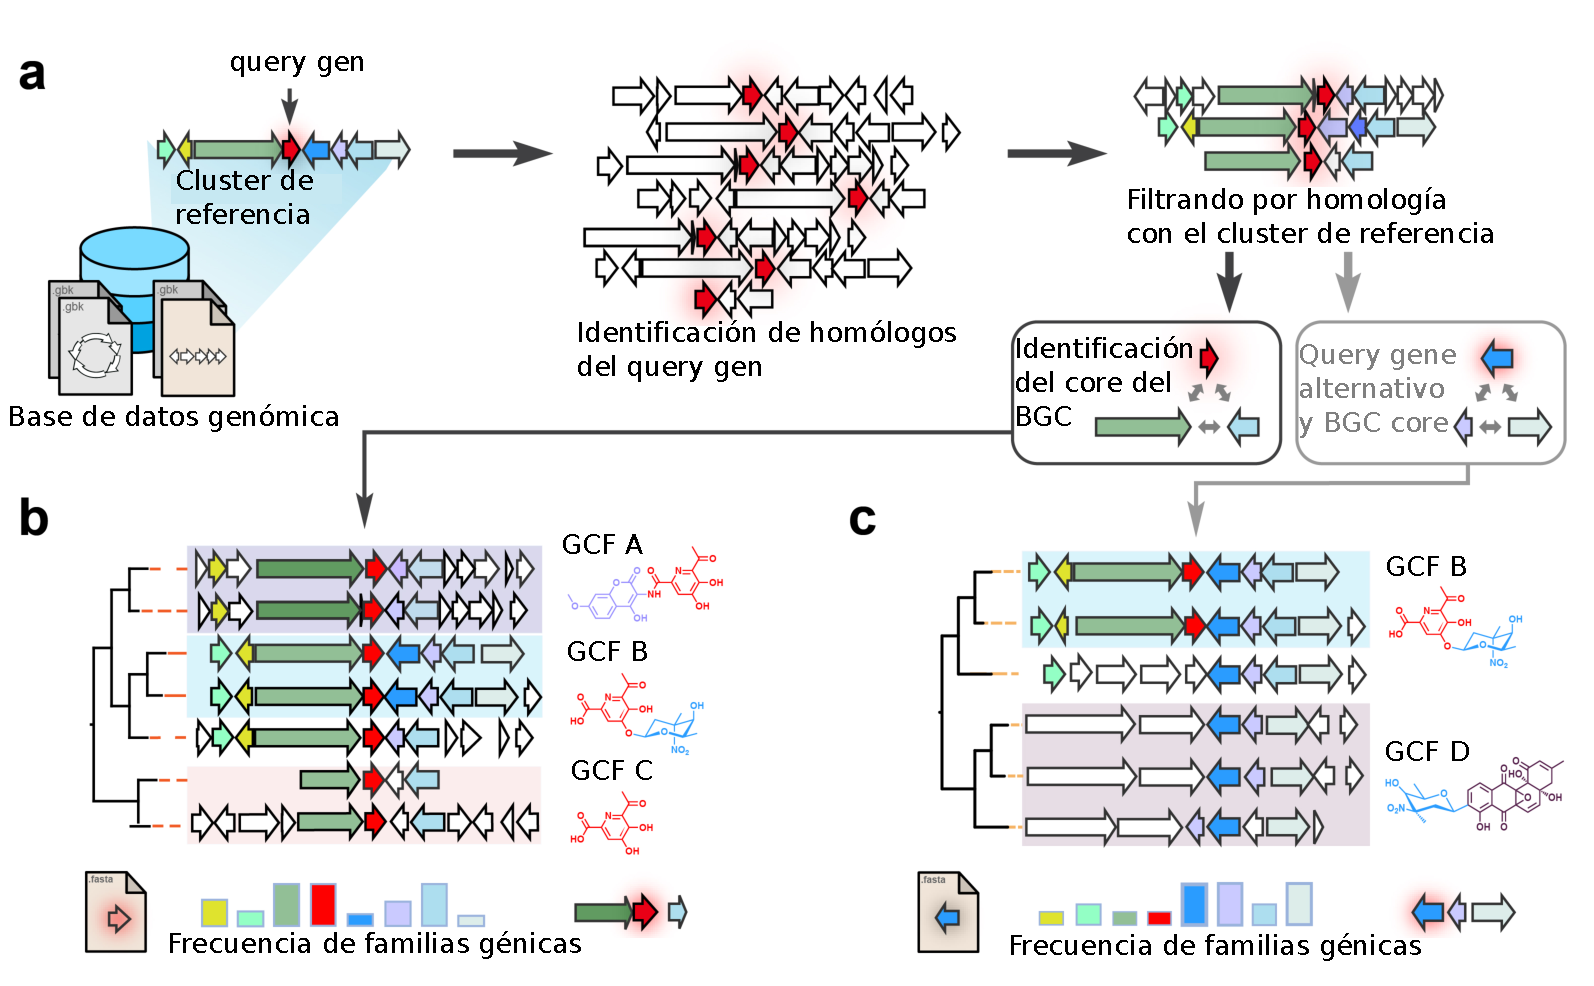
\includegraphics[angle = 0,scale = .6]{chapter3/Corason-pipe.pdf}
  \caption[La herramienta corason localiza familias de clusters biosintéticos en un linaje genómico partiendo de un cluster y un gen de referencia.]{\footnotesize{La herramienta corason localiza familias de clusters biosintéticos en un linaje genómico partiendo de un cluster y un gen de referencia. Todos los contextos genómicos que contengan ese gen y algún otro gen del cluster de referencia serán encontrados en el linaje seleccionado por el usuario. CORASON identifica el core génico de la familia. La información del core se utiliza para organizar filogenéticamente todos los miembros de la familia del BGC, es decir todas las variantes del BGC serán organizadas. El core génico está relacionado con el core de la molécula, la parte variable del BGC codifica enzimas accesorias que producen ornamentos i.e. variantes moleculares. Al cambiar de gen de referencia CORASON permite explorar otras familias de BGC que contengan las mismas modificaciones. Los resultados se presentan en una visualización que permite al mismo tiempo apreciar variación a nivel de presencia-ausencia de genes entre miembros de una familia de BGCs, como también apreciar variación a nivel de secuencia a través de un gradiente de color entre genes conservados entre una variante y el BGC de referencia.}}
  \label{fig:Corason-pipe}
  \end{figure}
  
  CORASON es una herramienta en línea de comandos para organizar
  filogenéticamente la variación de una familia de clusters, Figura
  \autoref{fig:Corason-pipe}. Dada la existencia de variantes de BGCs en
  bases de datos de linajes genómicos se diseñó CORASON. Corason se
  ejecuta en línea de comandos, su función es identificar el core génico
  de un BGC y utilizarlo para presentar una visualización de las variantes
  de la familia organizadas filogenéticamente
  
  Los métodos de minado de genomas han acelerado el descubrimiento de
  nuevos clusters biosintéticos (BGCs). Casi cada nueva bacteria que es
  secuenciada aporta alguna novedad al pangenoma bacteriano conocido. Una
  fracción de estos genes novedosos formará parte de variantes de BGCs
  previamente conocidos aportando diversidad a las familias de clusters
  biosintéticos. La diversidad genética que existe en las familias de BGCs
  está directamente relacionada con cambios moleculares, incluso pequeñas
  variantes en un metabolito pueden ocasionar diferencias en su función
  biológica.
  
  CORASON fue diseñado con las siguientes características: (i) una
  interfaz de línea de comando simple (ii) identificación del core génico
  del BGC (iii) la reconstrucción filogenética de la familia de BGCs
  utilizando la información del core (iv) salida visual en formato SVG,
  que muestra tanto la anotación funcional de los genes como como la
  distancia respecto a sus ortólogos del cluster de referencia.
  
  En este capítulo presento CORASON, CORe Analysis of Syntenic Orthologs
  to prioritize Natural products biosynthetic gene clusters, una
  herramienta para explorar la diversidad en el contenido de los BGCs así
  como su distribución en un linaje genómico proporcionado por el usuario.
  
  \section{Algoritmo y características de
  CORASON}\label{algoritmo-y-caracteristicas-de-corason}
  
  \begin{figure}[h!tbp]
  \centering
  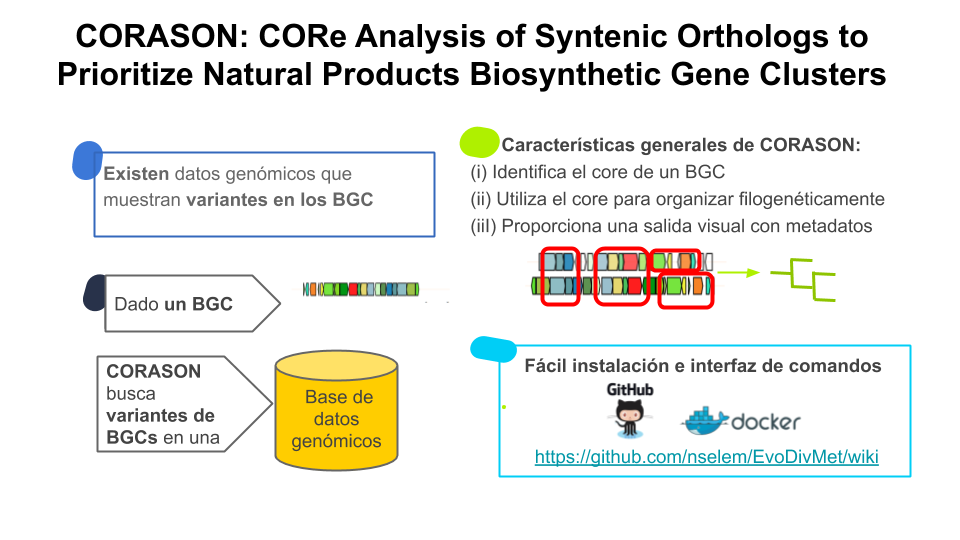
\includegraphics[angle = 0,scale = .4]{chapter3/ISBATalk.png}
  \caption[ CORASON es una herramienta en línea de comandos para organizar filogenéticamente la variación de una familia de clusters. ]{\footnotesize{CORASON es una herramienta en línea de comandos para organizar filogenéticamente la variación de una familia de clusters. Dada la existencia de variantes de BGCs en bases de datos  de linajes genómicos se diseñó CORASON. Corason se ejecuta en línea de comandos, su función es identificar el core génico de un BGC y utilizarlo para presentar una visualización de las variantes de la familia organizadas filogenéticamente}}
  \label{fig:ISBATalk}
  \end{figure}
  
  La herramienta corason, como se muestra en la \autoref{fig:ISBATalk}
  localiza familias de clusters biosintéticos en un linaje genómico
  partiendo de un cluster y un gen de referencia. Todos los contextos
  genómicos que contengan ese gen y algún otro gen del cluster de
  referencia serán encontrados en el linaje seleccionado por el usuario.
  CORASON identifica el core génico de la familia. La información del core
  se utiliza para organizar filogenéticamente todos los miembros de la
  familia del BGC, es decir todas las variantes del BGC serán organizadas.
  El core génico está relacionado con el core de la molécula, la parte
  variable del BGC codifica enzimas accesorias que producen ornamentos
  i.e.~variantes moleculares. Al cambiar de gen de referencia CORASON
  permite explorar otras familias de BGC que contengan las mismas
  modificaciones. Los resultados se presentan en una visualización que
  permite al mismo tiempo apreciar variación a nivel de presencia-ausencia
  de genes entre miembros de una familia de BGCs, como también apreciar
  variación a nivel de secuencia a través de un gradiente de color entre
  genes conservados entre una variante y el BGC de referencia.
  
  CORASON permite la rápida identificación de variantes de BGCs y organiza
  los resultados utilizando una aproximación filogenética. En la figura
  {[}CorasonPipeline{]} se muestra esquemáticamente como dado un cluster
  de referencia y un gen localizado en el cluster, así como las secuencias
  genómicas de un linaje de referencia corason buscará todas las variantes
  del cluster de referencia que existen en el linaje genómico
  seleccionado.
  
  \section{Las familias de BGCs están formadas por variantes del BGC de
  referencia.}\label{las-familias-de-bgcs-estan-formadas-por-variantes-del-bgc-de-referencia.}
  
  Así como existen familias génicas, un gen y todos sus homólogos,
  incluidos parálogos, ortólogos y xenólogos, también existen familias de
  BGCs. No es tan claro definir un BGC porque no tiene un codón de inicio
  y un codón de paro como un gen. En algunas ocasiones como en el caso de
  scytonemin todos los genes del BGC se expresan al recibir un estímulo,
  como los rayos UV en este caso. Otras veces en la producción del
  metabolito participan genes que no son necesariamente contiguos, y por
  ello al cambiar el BGC de organismo y realizar expresión heteróloga no
  se obtiene el mismo metabolito. Las fronteras es decir los genes de la
  orilla del BGC no siempre son claras.
  
  Así pues, cuando se habla de un BGC no se debe pensar que este es igual
  en todos los organismos del linaje, es decir que tiene el mismo
  contenido génico. Hay variación tanto a nivel de contenido génico como a
  nivel de secuencia entre los genes en común. Esta variación produce la
  promiscuidad de producto, una familia de BGCs produce distintos
  productos a partir de los mismos precursores. En este trabajo vamos a
  tomar como BGC de referencia a los anotados en MIBiG, que son de los que
  se tienen datos experimentales respecto al producto reportado. Todas sus
  variantes que contengan al menos dos genes en común, uno de referencia
  seleccionado por el usuario y otro cualquiera pero común con el BGC de
  referencia son considerados parte de la familia del BGC.
  
  Como ejemplo de familias de BGCs podemos pensar a los operones. Un
  operón es el conjunto de genes dedicados a la síntesis de algún
  metabolito del metabolismo central, estos genes suelen encontrarse
  juntos en el cromosoma y transcribirse simultáneamente. Ejemplos de
  estos operones son los que producen los aminoácidos histidina y
  triptófano. Estos ``BGCs'' hace millones de años fueron posiblemente
  parte del metabolismo especializado y debido a su éxito se fijaron en lo
  que ahora vemos como BGCs conservados en ciertos linajes genómicos. En
  estos casos las fronteras son claras y la variación génica es poca. Aún
  así existen otros ejemplos donde puede constatarse variación en las
  rutas de síntesis de mecanismos centrales de metabolismo procariota. En
  el caso de histidina y triptófano, como hablaremos en el siguiente
  capítulo, es la variación a nivel de secuencia y no a nivel de
  composición génica la que produce diversidad de producto.
  
  En oposición a los BGCs u operones de metabolismo conservado, están los
  BGCs del actual metabolismo especializado, así como se encuentran
  familias con mucha variación génica pueden encontrarse otras muy
  conservadas. En este capítulo presentaremos varios ejemplos de familias
  de BGCs.
  
  \section{Aplicaciones de CORASON en Actinobacteria y
  Pseudomonas}\label{aplicaciones-de-corason-en-actinobacteria-y-pseudomonas}
  
  En el capítulo anterior las variantes del BGC scytonemin en
  Cyanobacteria fueron encontradas al aplicar CORASON a dicho linaje. En
  este capítulo presento ejemplos del uso de CORASON para investigar los
  patrones de conservación/variación en familias de BGCs en los linajes
  Actinobacteria y \emph{Pseudomonas}. Primero, versiones iniciales de
  CORASON fueron usadas junto con cromatografía y espectrometría de masas
  (LC-MS) para estudiar la ecología y evolución de los sideróforos del
  tipo desferroxiaminas en Actinobacteria. Este estudio permitió la
  identificación de desG, un miembro de la familia penicilin amidasa
  responsable de la arilación de desferroxiaminas en actinomicetos
  acuáticos {[}REF{]}.
  
  En un segundo ejemplo, CORASON fue utilizado para investigar la
  existencia de variantes en Actinobacteria del cluster productor de
  arsenolípidos que se encuentra en \emph{Streptomyces lividans}. En la
  tercera aplicación, se investigó la distribución en Actinobacteria de un
  BGC de \emph{Streptomyces lividans} que es novedoso porque involucra una
  enzima que utiliza tRNA de la familia FemXAB. La predicción de producto
  de este BGC es un metabolito que contiene un grupo azoxy. Esta
  predicción ha sido confirmada utilizando LC-MS {[}Aguilar in prep{]} .
  
  Finalmente, un cuarto ejemplo es presentado: el de los contextos
  genómicos de \emph{tauD} que codifica una dioxigenasa involucrada en el
  metabolismo de taurina en su papel de enzima del metabolismo conservado.
  En Actinobacteria \emph{tauD} es parte de 15 BGCs reportados en MIBiG,
  aunque en \emph{Pseudomonas} no existen BGCs reportados EvoMining
  predice expansiones en este linaje genómico y CORASON predice
  conservación en los contextos genómicos de estas copias extra que
  guardan cierta similitud con variantes de los BGCs conocidos en
  Actinobacteria.
  
  Estos cuatro ejemplo ilustran como CORASON puede ser utilizado tanto
  para priorizar nuevos BGCs como para ligar la variación génica de
  familias de BGCs con diversidad estructural. CORASON es una expansión de
  las habilidades de EvoMining {[}cruz-morales{]} de encontrar enzimas en
  el proceso de diversificación funcional. CORASON encuentra familias de
  BGCs, y presenta una rápida visualización de sus variantes. Ambas
  herramientas fueron desarrolladas para expandir nuestro conocimiento
  sobre nueva química mediante la genómica comparativa. CORASON está
  disponibles en su contenedor de docker en github
  \url{https://github.com/nselem/corason}.
  
  \section{Estas familias pueden
  clasificarse}\label{estas-familias-pueden-clasificarse}
  
  Variantes del cluster biosintético de desferroxiamina \autoref{fig:des}
  fueron identificadas por CORASON en Actinobacterias de cuatro ciénegas.
  Una variante del BGC de desferroxiamina fue identificada. Esta variante
  se diferencia del cluster reportado por la ganancia de una penicilin
  amidasa. A este gen extra se le llamó \emph{desG}. Fue verificado que la
  variación génica está ligada con la variación molecular
  
  El hierro es necesario en el metabolismo de muchos seres vivos. Para
  poder utilizarlo las bacterias han desarrollados moléculas captadoras de
  hierro llamadas sideróforos. Un ejemplo de sideróforo es la molécula de
  desferroxiamina sintetizada por los genes \emph{des} en Actinobacteria
  
  \begin{figure}[h!tbp]
  \centering
  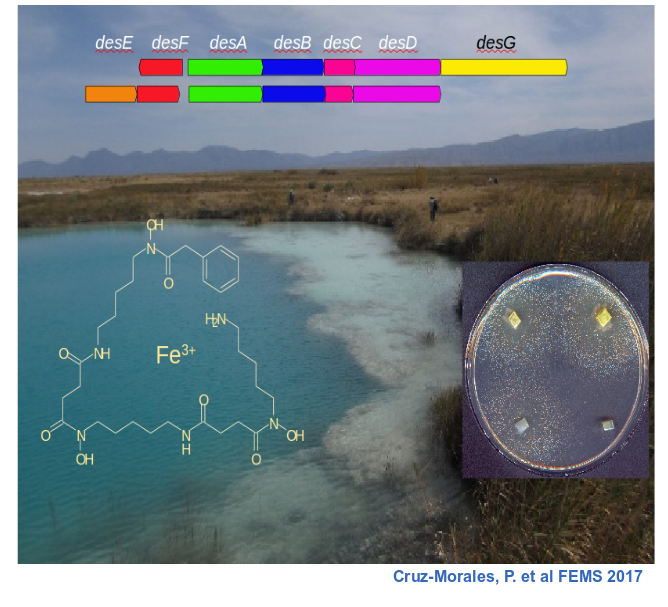
\includegraphics[angle = 0,scale = .4]{chapter3/des.png}
  \caption[EvoMining Algorithm]{\footnotesize{Variantes del cluster biosintético de desferroxiamina fueron identificadas por CORASON en Actinobacterias de cuatro ciénegas. Una variante del BGC de desferroxiamina fue identificada. Esta variante se diferencia del cluster reportado por la ganancia de una penicilin amidasa. A este gen extra se le llamó $desG$. Fue verificado que la variación génica está ligada con la variación molecular}}
  \label{fig:des}
  \end{figure}
  
  \section{Un BGC reportado puede tener muchas variantes que conforman una
  familia de
  BGCs}\label{un-bgc-reportado-puede-tener-muchas-variantes-que-conforman-una-familia-de-bgcs}
  
  En el linaje de \emph{Streptomyces} EvoMining obtuvo como predicción una
  arsenoenol piruvato sintasa en una rama del árbol de expansiones de la
  familia 3-fosfoshikimato-1-carboxivinyl transferasa (AroA). Estudios de
  mutagénesis y de expresión diferencial génica en presencia de arsénico
  confirmaron que en \emph{Streptomyces coelicolor} y en
  \emph{Streptomyces lividans} esta enzima pertenece a un BGC que
  sintetiza arsenolípidos {[}Pablo tesis{]}. El contexto genómico de AroA
  en estos organismos incluye una enzima PKS localizada a seis genes de
  distancia. AntiSMASH predice los BGCs tipo PKS de estas enzimas pero no
  incluye en ellos a la arsenoenol piruvato sintasa. El valor de EvoMining
  fue descubrir que esta copia extra de AroA estaba dedicada al
  metabolismo especializado y por tanto bien podía tener su propiio BGC o
  dada la cercanía con las PKS podía ser parte de estos PKS-BGCs. Esta
  ruta de síntesis de arseno compuestos, fue descubierta a partir de una
  rama de copias extra de AroA donde se apreciaba diversidad en las
  secuencias de aminoácidos. Una pregunta posible es si esta diversidad de
  secuencia a nivel de enzima ascendía a un siguiente nivel. Es decir si
  también existe diversidad a nivel del BGC, si se encuentran variantes
  con distintos patrones de presencia/ausencia en los genes que coponen al
  BGC de \emph{S coelicolor}. O más aun, quedaba por investigar si el BGC
  tenía cierto grado de conservación o era exclusivo de estos dos
  organismos \emph{S. coelicolor y S. lividans}
  
  Una versión preliminar de CORASON, permitió visualizar las variantes de
  los contextos genómicos de las arsenol piruvato sintasas. Los genomas
  donde se buscaron estas variantes fueron seleccionados por una búsqueda
  de blast en NCBI en la base de datos no redundante como aparecía en
  2016. Después de organizar manualmente los BGCs como se muestran a la
  izquierda de la {[}Fig Arseno-BGC{]}, la visualización permitió
  distinguir 4 grupos de contextos conservados. El primero independiente
  de PKS y NRPS mostrado en morado, el segundo con una NRPS-PKS híbrida
  mostrado en un rectángulo verde y finalmente en rosa y naranja se
  muestran los grupos tercero y cuarto que contienen una PKS, los primeros
  del lado izquierdo y los segundos del lado derecho. Presumiblemente
  estos BGCs aunque contienen un core común producen distintos arseno
  compuestos.
  
  \begin{figure}[h!tbp]
  \centering
  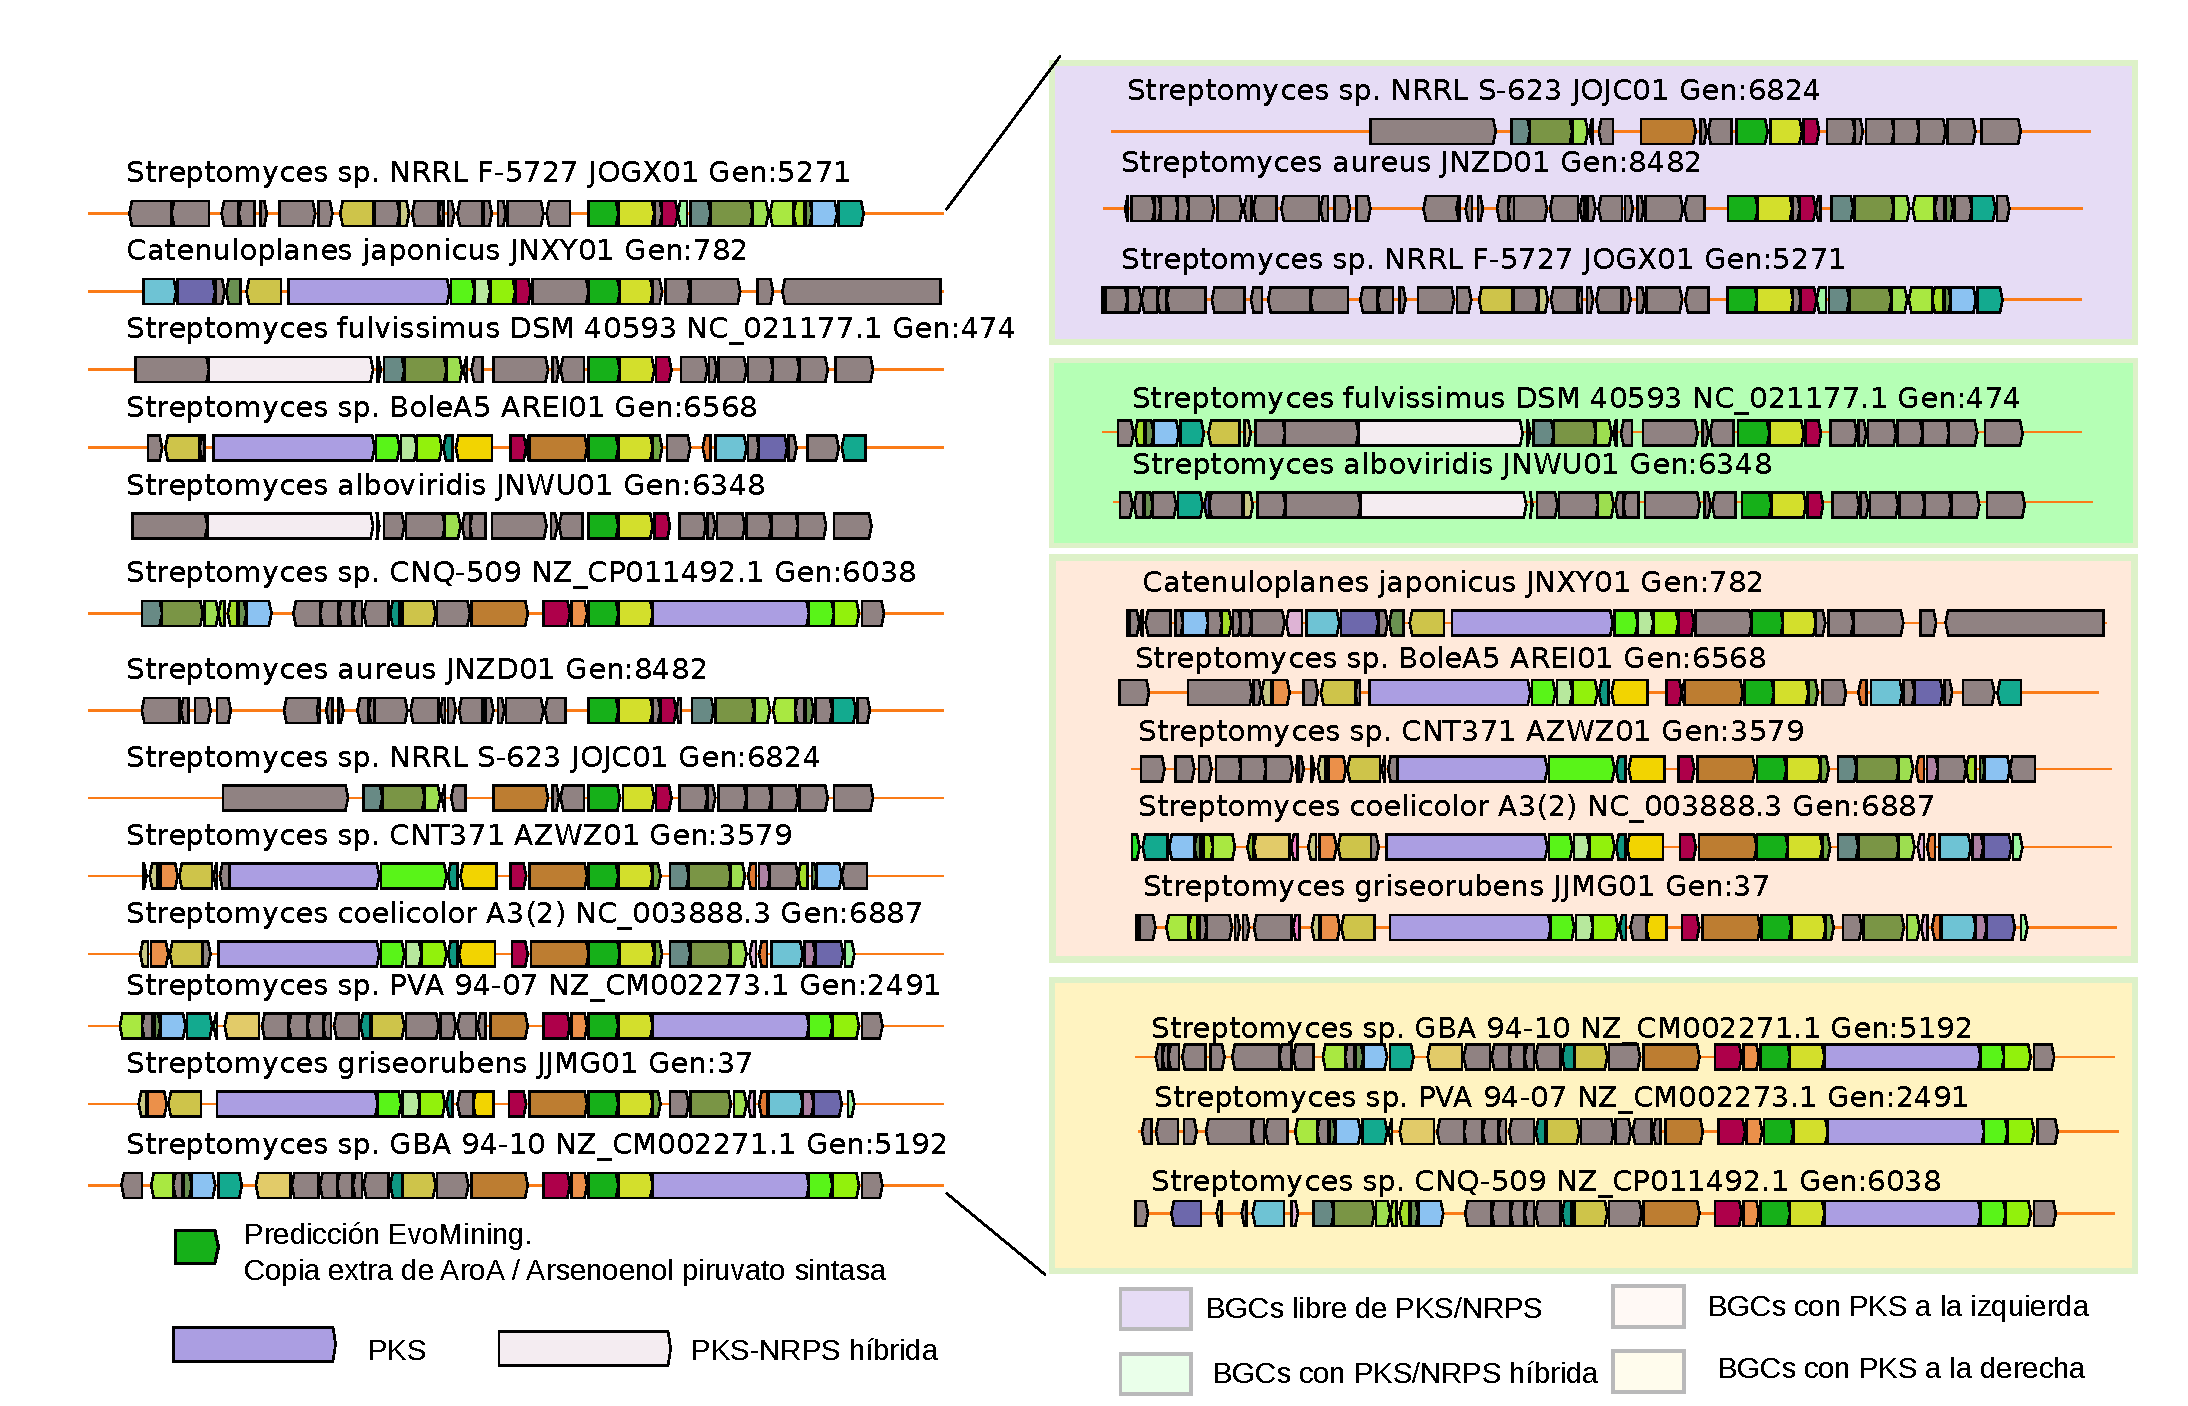
\includegraphics[angle = 0,scale = .4]{chapter3/Coelicolor.pdf}
  \caption[EvoMining Algorithm]{\footnotesize{Contexto genómico conservado en las expansiones de AroA. La arsenoenol piruvato sintasa fue descubierta en un árbol de EvoMining como parte de una rama de expansiones de AroA en Actinobacteria. El contexto genómico de la arsenoenol piruvato sintasa de $S.~coelicolor$ tiene un core conservado en Actinobacteria. Este BGC está dedicado a la síntesis de metabolitos secundarios de tipo arsenolípidos. Primero se identificaron en otras secuencias genómicas contextos que contengan el homólogo de AroA y algún otro gen de su vecindad en $S.~coelicolor$. A continuación, se ordenaron manualmente los contextos obtenidos y se pudo identificar al menos cuatro diferentes clases de BGCs. La primera clase mostrada en un rectángulo morado no contiene PKS o NRPS, la segunda enmarcada en verde contiene una PKS-NRPS híbrida. La tercera clase incluye una PKS a la izquierda y a más de cinco genes de distancia de la Arsenoenol piruvato sintasa y finalmente la última clase contiene una PKS a la derecha y a sólo un gen de distancia de esta enzima. Esta figura muestra que existen variantes de un BGC }}
  \label{fig:Coelicolor}
  \end{figure}
  
  El contexto genómico conservado en las expansiones de AroA puede
  apreciarse en la \autoref{fig:Coelicolor}. La arsenoenol piruvato
  sintasa fue descubierta en un árbol de EvoMining como parte de una rama
  de expansiones de AroA en Actinobacteria. El contexto genómico de la
  arsenoenol piruvato sintasa de \_S. coelicolor \_tiene un core
  conservado en Actinobacteria. Este BGC está dedicado a la síntesis de
  metabolitos secundarios de tipo arsenolípidos. Primero se identificaron
  en otras secuencias genómicas contextos que contengan el homólogo de
  AroA y algún otro gen de su vecindad en \emph{S. coelicolor}. A
  continuación, se ordenaron manualmente los contextos obtenidos y se pudo
  identificar al menos cuatro diferentes clases de BGCs. La primera clase
  mostrada en un rectángulo morado no contiene PKS o NRPS, la segunda
  enmarcada en verde contiene una PKS-NRPS híbrida. La tercera clase
  incluye una PKS a la izquierda y a más de cinco genes de distancia de la
  Arsenoenol piruvato sintasa y finalmente la última clase contiene una
  PKS a la derecha y a sólo un gen de distancia de esta enzima. Esta
  figura muestra que existen variantes de un BGC
  
  La visualización realizada para los arsenolípidos no incluía ningún tipo
  de orden y era difícil distinguir grupos de BGCs. Por esta razón se
  pensó que el orden filogenético ya no de una enzima sino de el core del
  BGC ordenaría las variantes del BGC. Este orden mostraría en un continuo
  la dinámica genómica del BGC establecida por los procesos evolutivos. En
  el caso de los arsenolípidos se utilizó Orthocore para la identificación
  del core del BGC. En las siguientes versiones de CORASON esta
  característica fue implementada como parte del algoritmo.
  
  \section{CORASON analiza la conservación del contexto genómico de los
  EvoMining
  hits}\label{corason-analiza-la-conservacion-del-contexto-genomico-de-los-evomining-hits}
  
  La predicción de un BGC para la síntesis de un compuesto tipo azoxy es
  otro ejemplo de CORASON como complemento de EvoMining para la
  identificación de los dos niveles de promiscuidad, tanto a nivel familia
  enzimática como familia de BGCs \autoref{fig:azoxy}. Este trabajo se
  encuentra en preparación para su publicación por Aguilar-Martínez.
  
  \begin{figure}[h!tbp]
  \centering
  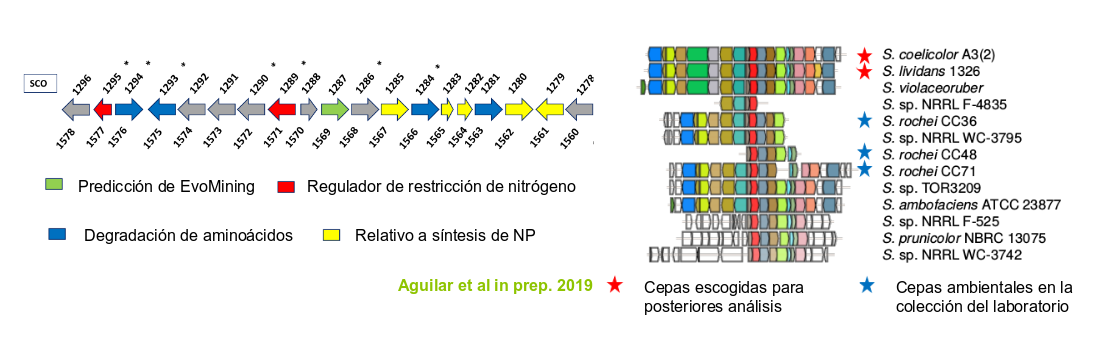
\includegraphics[angle = 0,scale = .4]{chapter3/azoxy.png}
  \caption[EvoMining Algorithm]{\footnotesize{Azoxy BGC}}
  \label{fig:azoxy}
  \end{figure}
  
  \clearpage
  
  \section{\texorpdfstring{El contexto de una rama divergente de
  \emph{tauD} está conservado en
  Pseudomonas}{El contexto de una rama divergente de tauD está conservado en Pseudomonas}}\label{el-contexto-de-una-rama-divergente-de-taud-esta-conservado-en-pseudomonas}
  
  En Pseudomonas el gen \emph{tauD} tiene un contexto que incluye genes de
  metabolismo especializado. Variantes de este contexto están distribuidas
  en varios organismos \autoref{fig:PseudomonasTauD} . Parecen ser
  diferentes de los rimosamides y detoxins reportados en Actinobacteria.
  
  \begin{figure}[h!tbp]
  \centering
  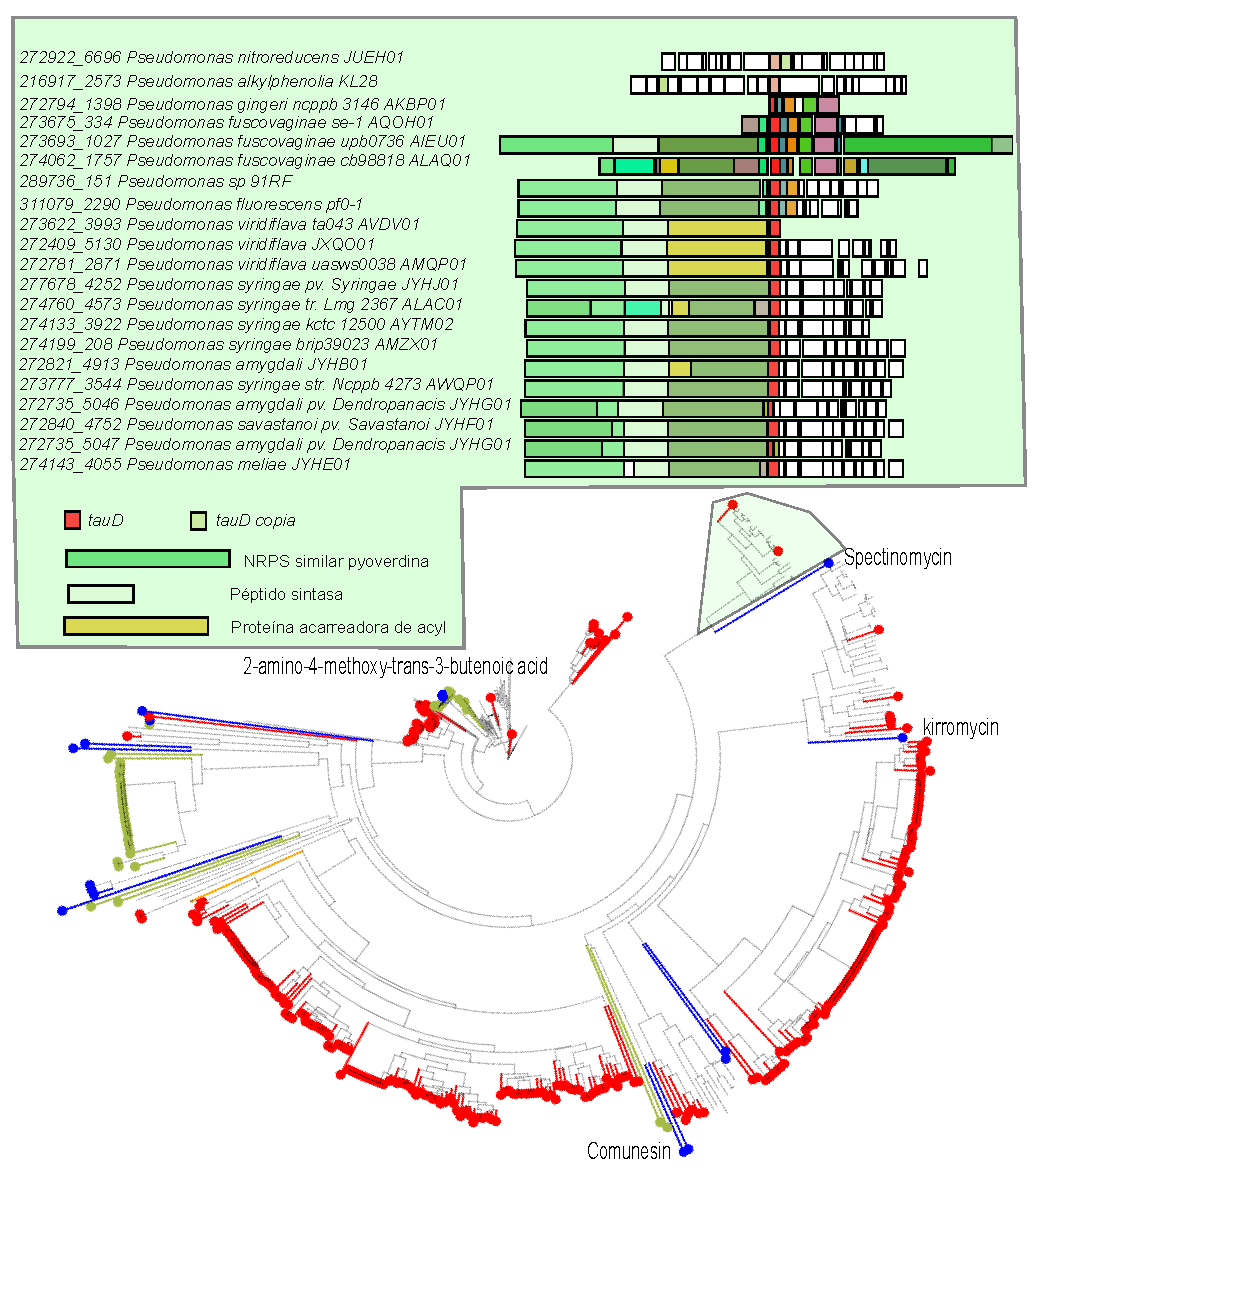
\includegraphics[angle = 0,scale = .9]{chapter3/PseudomonasTauD.pdf}
  \caption[EvoMining Algorithm]{\footnotesize{En Pseudomonas el gen $tauD$ tiene un contexto que incluye genes de metabolismo especializado. Variantes de este contexto están distribuidas en varios organismos. En particular  }}
  \label{fig:PseudomonasTauD}
  \end{figure}
  
  \section{CORASON se adaptó a la herramienta BiG-SCAPE de clasificación
  de familias de
  BGCs}\label{corason-se-adapto-a-la-herramienta-big-scape-de-clasificacion-de-familias-de-bgcs}
  
  BIG-SCAPE es una herramienta bioinformática para separar un conjunto de
  BGCs en familias de acuerdo al contenido, conservación y distribución de
  sus dominios. Un dominio es un conjunto de secuencia conservado de un
  gen, es considerado una unidad de las proteinas. CORASON complemento
  BIG-SCAPE \autoref{fig:CORASONAlgorithm} al proporcionar un algoritmo
  para ordenar la diversidad dentro de la familia. A la vez CORASON
  permite conectar mediante la evolución a familias aparentemente
  separadas por BiGSCAPE.
  
  \begin{figure}[h!tbp]
  \centering
  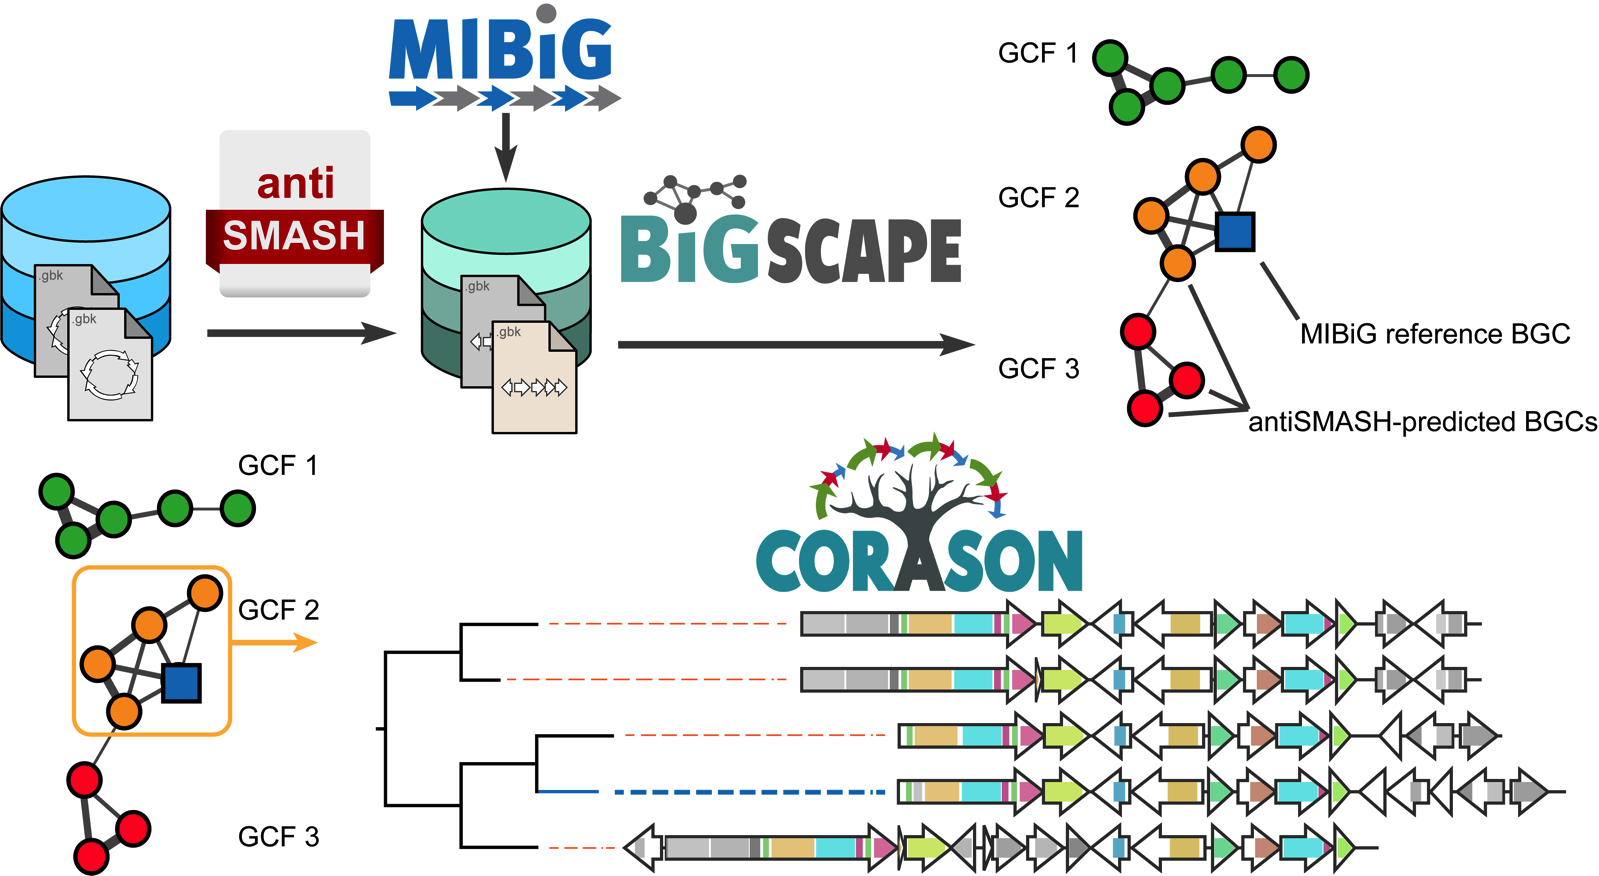
\includegraphics[angle = 0,scale = .3]{chapter3/corason_fig1.png}
  \caption[Algoritmo de CORASON Algorithm]{\footnotesize{}}
  \label{fig:CORASONAlgorithm}
  \end{figure}
  
  \section{BiG SCAPE y CORASON identificaron nuevos productos variantes de
  la familia de BGCs Rimosamide - Detoxin en
  Actinobacteria}\label{big-scape-y-corason-identificaron-nuevos-productos-variantes-de-la-familia-de-bgcs-rimosamide---detoxin-en-actinobacteria}
  
  En esta sección utilizamos CORASON y BIG-SCAPE para analizar una base de
  datos de miles de genomas de ACtinobacteria. Con estas herramientas se
  organizó la diversidad biosintética de las familias de BGC detoxin y
  rimosamide {[}\protect\hyperlink{ref-mcclure_elucidating_2016}{166}{]}.
  El análisis reveló diversidad tanto en los géneros de los organismos que
  contienen a esta familia, y en la composición génica del BGC. Entre los
  géneros con alguna variante del BGC están Amycolatopsis, Streptomyces.
  El core conservado de los BGCs detoxin y rimosamide está compuesto por
  una NRPS, una NRPS/PKS híbrida, y un homólogo de tauD. Este homólogo fue
  sugerido por un análisis de EvoMining. En \emph{E.coli} tauD se
  encuentra en el operón tauABCD {[}MM1{]} La ruta de síntesis de
  rimosamide difiere de la de detoxins porque tiene una NRPS adicionoal,
  que codifica para una modificación del core de molecula
  detoxin/rimosamide con isobutyrate y glycine39.
  
  \begin{figure}[h!tbp]
  \centering
  \includegraphics[angle = 0,scale = .8]{chapter3/figura5.pdf}
  \caption[Rimosamide]{\footnotesize{Rimosamide}}
  \label{fig:Rimosamide}
  \end{figure}
  
  El hecho de que el gen \emph{tauD} estuviera presente en todos los
  miembros de la familia \autoref{fig:Rimosamide} captó nuestra atención.
  El producto del gen tauD pertenece a la super familia de enzimas
  Fe(II)/\(\alpha\)-ketoglutarato-dependientes hidroxilasas. En particular
  tauD codifica una \(\alpha\)-ketoglutarato-dependendiente taurina
  dioxigenasa involucrada en la asimilacion de sulfito por la liberación
  oxigenolítica del aminoácido taurina41. Interesantemente, esta familia
  también incluye enzimas en linajes como hongos, bacterias y plantas.
  Dichas enzimas catalizan hydroxylations, desaturations, ring expansions
  and ring formations, among other chemical transformations. A la fecha,
  el rol de TauD en la biosíntesis de los metabolitos detoxin y rimosamide
  aún es desconocido, se ha sugerido que es responsable de la oxidación de
  la prolina observada en algunos análogos39.
  
  Para identificar variantes de los BGCs relacionados a detoxin y
  rimosamide dentro de la rama de metabolismo especializado los 1175 BGCs
  del dataset que contenían un homólogo de tauD se pasaron por un análisis
  combinado de BiG-SCAPE/CORASON. Los BGCs fueron procesados con CORASON
  usando tauD como query gene. Teniendo como resultado que es el único
  miembro del `BGC core'. Es importante notar que el core del BGC puede
  contener entre 1 y 3 genes, {[}La NRPS, y la NRPS-PKS híbrida quedan en
  este ejemplo fuera del core debido a gaps en la secuencia del genoma de
  organismos como \emph{Streptomyces humi}, \emph{Streptomyces
  Spectabilis} y \emph{Amycolatopsis Vancoresmycina}{]}
  
  \section{CORASON sugiere que las familias detoxin y rimosamide
  pertenecen a un amplio clan de familias dedicadas a la síntesis de
  péptidos.}\label{corason-sugiere-que-las-familias-detoxin-y-rimosamide-pertenecen-a-un-amplio-clan-de-familias-dedicadas-a-la-sintesis-de-peptidos.}
  
  El análisis de CORASON reveló que las familias de los BGCs detoxin y
  rimosamide GCFs identificados en BiG-SCAPE eran parte de todo un clan de
  biosintesis de péptidos que incluía clados inexplorados {[}MM10{]} del
  phylum Actinobacteria {[}Fig TauDActinobacteria{]}. La organización
  filogenética de los BGCs provista por CORASON, reveló familias de BGCs
  que fueron omitidas debido al umbral utilizado por el algoritmo de
  clustering de BiG-SCAPE. Esto debido a la cercanía de genes
  biosintéticos detectados por antiSMASH como suficientemente diferentes
  como para ser clasificados en otras familias (ver Fig. S10).
  
  Hipotetizamos que las detoxins codificadas por los BGCs en los clados
  inexplorados contendrán cierta novedad química relacionada con las
  variaciones genéticas. Afortunadamente, 40 de las 152 cepas
  identificadas como portadoras de un BGCs estaban representadas en
  nuestros datos metabolómicos de 363--cepas por LC-MS/MS. Análisis de
  redes moleculares de estos datos indicaron la presencia de tres detoxin
  conocidas, cuatro rimosamide conocidas y otras 103 variantes de detoxin
  o rimosamide (Fig. 3c), el basto universo químico sugerido por el
  análisis BiG-SCAPE/CORASON.
  
  \section{Clados selectos del árbol de CORASON que contiene a las
  familias rimosamide/detoxin contienen diversidad génica que correlaciona
  con novedad
  química.}\label{clados-selectos-del-arbol-de-corason-que-contiene-a-las-familias-rimosamidedetoxin-contienen-diversidad-genica-que-correlaciona-con-novedad-quimica.}
  
  Tres de los clados que codifican para detoxin BGC fueron identificados
  por BiG-SCAPE dentro del árbol de CORASON capturaron nuestro interés
  ({[}Fig TauDActinobacteria{]}, in colored boxes). En esta sección se
  describe el trabajo experimental realizado por Michael Mulloney del
  grupo de colaboradores de West Chicago, de los tres clados y
  específicamente de los organismos que seleccioné como candidatos a
  presentar diversidad química.
  
  \subsection{El clado P450/enoyl agrega una heptanamida al core molecular
  detoxin/rimosamide}\label{el-clado-p450enoyl-agrega-una-heptanamida-al-core-molecular-detoxinrimosamide}
  
  El primer clado es el `P450/enoyl clade' contiene genes como el
  citocromo P450 y un enoyl-CoA hydratasa/isomerasa dentro de cada uno de
  sus BGCs. Este clado está marcado en rojo {[}Fig TauDActinobacteria{]}.
  Análisis de datos por tandem MS de extractos de \emph{Streptomyces} sp.
  NRRL S-325, que se encuentra dentro de este clado, llevó al
  descubrimiento de la detoxin S1 (1; Fig TauDActinobacteria, S16--17).
  Este nuevo análogo contiene una cadena lateral de heptanamide, una
  extrucutra única entre las detoxins y rimosamides cuya instalación
  posiblemente depende de la enzima enoyl-CoA hydratase/isomerase.
  
  \subsection{El superclado spectinomycin/ detoxin-rimosamide-clan produce
  cinco variantes de
  detoxin.}\label{el-superclado-spectinomycin-detoxin-rimosamide-clan-produce-cinco-variantes-de-detoxin.}
  
  El segundo clado de interés,fue nombrado el `supercluster clade' (Fig.
  5, en verde claro), comprende los BGCs con genes de detoxin adjacentes
  al cluster que produce spectinomycin42 {[}Fig TauDActinobacteria{]}. El
  cluster de spectinomycin (MIBiG BGC0000715) contiene en su periferia al
  gen tauD como se muestra en la línea gris punteada de la {[}Fig
  TauDActinobacteria{]}. La secuencia del cluster de spectinomycin
  depositada en MIBiG es la única secuencia dsponible de
  \emph{Streptomyces spectabilis} NRRL 2792. Como no se sabe que tauD
  participe en la síntesis de spectinomycin se hipotetizó que pueden
  existir los genes del cluster de detoxin al lado de los genes del BGC de
  spectinomycin en \emph{S. spectabilis} NRRL 2792. Adquirimos esta cepa
  para determinar si el análisis de CORASON podía ayudar a la predicción
  de detoxin basado solamente en la presencia del query gen pero en
  ausencia completa de la secuencia del BGC de detoxin. Análisis en tandem
  de espectrometría de masas de extracto \emph{S. spectabilis} NRRL 2792
  reveló la producción de cinco compuestos tipo detoxin, incluyendo
  detoxin N1 (2; Fig TauDActinobacteria, S15), detoxin N2 (3; Fig. S15) y
  su análogo acetoxylated, detoxin N3 (4; Fig. S15).
  
  Los tiempos de retención de ionies y los patrones de fragmentación de
  los últimos dos compuestos también fueron observados en extractos de
  \emph{Streptomyces} sp. NRRL B-1347 parte del clado del supercluster,
  confirmando la habilidad de CORASON para guiar un descubrimiento,
  mediante la utilización de la filogenia a pesar de lo limitado de los
  datos en la cepa NRRL-2792. Análisis de LC-MS de cultivos de NRRL-2792
  suplementados con isotopos estables etiquedatos de amino acidos
  corroboraron las predicciones estructurales basadas en los análisis de
  la cepa cercana \emph{Streptomyces} sp. NRRL B-1347 (Fig
  TauDActinobacteria, S26--31). Los tres nuevos análogos incorporan
  copletamente el 13C6-isoleucine, pero d7-proline solo es incorporado en
  el compuesto 3. La pérdida de un deuterio de d7-proline en 2 y 4 soporta
  la asignación de acetoxylation del anillo de pyrrolidine común en
  detoxins y rimosamides39,43--45. Características especiales únicas a la
  serie de N-detoxins incluyen la incorporación de una tirosina
  N-formylated en 3 y 4 en lugar de fenilalanina, el residuo típico de
  detoxin/rimosamide, lo que es soportado por la incorporación del anillo
  d4-tyrosine. El compuesto 2 la incorporación única de un residuo
  derivado del triptofano en esta posición, haciendo evidente la retención
  de cuatro deuterios cuando en experimentos de alimentación de
  indole-d5-tryptophan (Fig. S27). Aunque los datos de MS fueron
  insuficientes para desenmascarar esta estructura, el compuesto 2 fue
  producido por \emph{S. spectabilis} NRRL 2792 en suficiente abundancia
  para el aislamiento y la elucidación estructural por NMR. Varios
  experimentos 1D y 2D confirmaron las asignaciones por datos de MS y
  establecieron una N-acetylated kynurenine como la estructura derivada de
  triptófano en 2 (Figs. S18-S27).
  
  \subsection{\texorpdfstring{El clado \emph{Amycolatopsis P450} produce
  cinco variantes de
  detoxin.}{El clado Amycolatopsis P450 produce cinco variantes de detoxin.}}\label{el-clado-amycolatopsis-p450-produce-cinco-variantes-de-detoxin.}
  
  El tercer clado que se estudió del super clan al que pertenecen las
  familias rimosamide-detoxin, contiene BGCs casi enteramente provenientes
  del género Amycolatopsis. Este clado está marcado en morado en la {[}Fig
  TauDActinobacteria{]}. Este clado de BGCs también contienen un gen P450
  único entre los BGCs del árbol, así que fue llamado el clado
  `Amycolatopsis/P450 clade'. Aunque no se contaba con datos metabolómicos
  de las cepas del clado de BGCs definidos por BiG-SCAPE como una gen
  cluster family (GCF), la visualización filogenética de CORASON permitió
  la selección de una cepa de Amycolatopsis de la que se tenían datos
  metabolómicos con un BGC muy similar, y que también contiene el gen P450
  ({[}Fig TauDActinobacteria{]}, línea gris cerca del clado
  \emph{Amycolatopsis}/P450 ). Análisis de datos de tandem MS de extracto
  fermetado de \emph{Amycolatopsis jejuensis} NRRL B-24427 reveló isómeros
  de detoxins P1 (5; {[}Fig TauDActinobacteria{]}, S15) que contienen
  tirosina, P2 (6; {[}Fig TauDActinobacteria{]}, S15) mostrando
  fenilalanina y una valina hidroxilada, así como la detoxin P3, un
  análogo cercano libre de hidroxilación (7; {[}Fig TauDActinobacteria{]},
  S15). Una validación de la asignación de aminoácidos observados en los
  patrones de fragmentación de MS/MS se consiguió mediante el uso de
  experimentos de incorporación de isótopos estables etiquetados de
  aminoácidos (Figs. S33--S36, S38--S41, and S43--S44).
  
  \section{CORASON permitió expandir las capacidades de EvoMining y
  explorar la promiscuidad de familias de BGCs de enzimas divergentes de
  metabolismo
  central.}\label{corason-permitio-expandir-las-capacidades-de-evomining-y-explorar-la-promiscuidad-de-familias-de-bgcs-de-enzimas-divergentes-de-metabolismo-central.}
  
  Nuestros resultados ilustran como BiG-SCAPE puede identificar conjuntos
  de BGCs relacionados, en un gran número de secuencias de genomas. Además
  al usar CORASON para reconstruir las filogenias de BGC para ordenar
  visualmente la evolución de un cluster biosintético y su diversidad
  proveen herramientas poderosas para el descubrimiento de nuevos clados
  de BGC que codifican en consecuencia para nueva quimica. Respecto a los
  BGCs detoxin/rimosamide, CORASON mostró habilidad para ayudar a minar
  bases de datos genómicas y descubrir siete nuevas detoxins.
  Específicamente, la organización de de las variantes de los BGC facilitó
  la identificación de los correspondientes variaciones en la estructura
  química -la presencia de un enoyl-CoA hidratasa/isomerasa corresponde a
  la familia de amida ácido graso detoxin S1 y la presencia de un gen P450
  corresponde a la presencia de hidroxilaciones en detoxins P1--P3.
  
  \subsubsection{Discusión}\label{discusion}
  
  El cluster des está muy conservado, no así los de arsenolípidos, ni los
  de rimosamide
  
  \chapter{La familia PriA}\label{la-familia-pria}
  
  \begin{figure}[h!tbp]
  \centering
  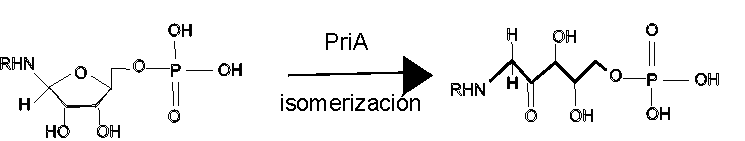
\includegraphics[angle = 0,scale = 1]{chapter4/isomerizacion.pdf}
  \caption[La reacción que cataliza PriA es una isomerización donde abre un anillo de cinco carbonos.]{\footnotesize{La reacción que cataliza PriA es una isomerización donde abre un anillo de cinco carbonos.}}
  \label{fig:isomerizacion}
  \end{figure}
  
  PriA es una familia de enzimas de Actinobacteria homóloga a la familia
  HisA en Enterobacteria. Según las definiciones de este trabajo PriA es
  una familia promiscua. Varios miembros de PriA han sido sujetos a
  estudios de cinéticas enzimáticas demostrándose su capacidad de
  catalizar tanto la reacción correspondiente a HisA como la de TrpF. Es
  decir PriA participa a la vez en las rutas de síntesis de Histidina y
  Triptofano, al menos en varias Actinobacterias. Los primeros miembros
  caracterizados como promiscuos en esta familia en el 2003 fueron
  \emph{Streptomyces coelicolor} y \emph{Mycobacterium tuberculosis}
  {[}\protect\hyperlink{ref-baronagomez_occurrence_2003}{5}{]}. La mayoría
  de las actinobacterias han perdido el gen trpF en la ruta del
  triptofano, por lo que se cree que la promiscuidad de PriA está
  extendida en un gran subconjunto de Actinobacteria. PriA en la ruta de
  histidina isomeriza el sustrato ProFAR en PRFAR, realizando la función
  HisA. En la ruta de triptofano lleva a cabo la isomerización de PRA en
  CdRP actuando análogamente a la función TrpF en la ruta del triptófano.
  En \emph{Streptomyces coelicolor} varios genes de los operones de
  histidina y triprofano están en la vecindad genómica de PriA.
  
  Además, en Actinobacteria PriA ha mostrado un gradiente funcional. Esta
  variación divide a la familia en varias subfamilias según su capacidad
  catalíticas en los sustratos ProFAR y PRA. En la \autoref{tab:cineticos}
  se muestra la constantes catalíticas de PriA estimadas en diferentes
  organismos para estos dos sustratos. Estos datos ejemplifican las
  subfamilias de PriA, en la tabla se encuentran ejemplos de miembros de
  PriB, la subfamilia ubicada en el género \emph{Streptomyces} con baja
  capacidad de catálisis para la función TrpF. Varios \emph{Streptomyces}
  con un ortólogo en la familia PriB, se diferencian de otras
  Actinobacterias en que contienen en su genoma un gen \emph{trpF}
  localizado fuera del contexto genómico inmediato de los operones de
  histidina y triptofano. Otra subfamilia de PriA es subHisA, que ha
  perdido totalmente la actividd TrpF, existen miembros de subHisA en
  \emph{Corynebacteria} y en \emph{Actinomyces}. Finalmente en Actinomyces
  encontramos la subfamilia \emph{subTrpF} que ha perdido la actividad de
  HisA.
  
  En este capítulo en las siguientes secciones se exploran cuatro apectos
  de la familia PriA. \emph{i)} La distribución y el contexto genómico de
  PriA en diversos linajes genómicos. \emph{ii)} La información contenida
  a nivel de aminoácidos en variantes de PriA como medio de studio de
  rutas evolutivas y su relación con la reconstrucción de su estructura
  tridimensional. \emph{iii)} Las posibles afinidades de PriA por otros
  sustratos con métodos bioinformáticos, y finalmente \emph{iv)} La
  validación experimental de PriA en sustratos diferentes de PRA y ProFAR
  o bien en combinaciones de los mismos.
  
  \begin{longtable}[]{@{}l@{}}
  \caption{Reclutamientos de expansiones de PriA en MIBiG
  \label{tab:cineticos}}\tabularnewline
  \toprule
  --------------------------------------------------------------------------\tabularnewline
  \bottomrule
  \end{longtable}
  
  \clearpage    
  
  \begin{landscape}  
  
  $$
  \resizebox{\columnwidth}{!}{%
  \begin{tabular}{ l c r c c c c c c c l}
  \hline \\ [-1.5ex]
  Fuente  &Familia & HisA $in\hspace{.1cm}vivo$ &TrpF $in\hspace{.1cm}vivo$ & $K{cat}^{ProFAR}[M^{-1}s^{-1}]$ & $Km^{ProFAR}[\mu M]$& $\frac{K{cat}}{Km} ProFAR$ & $K{cat}^{PRA}[M^{-1}s^{-1}]$ & $Km^{PRA}[\mu M]$  &  $\frac{Kcat}{Km} PRA $  &Referencia  \\ [1ex]
  \hline \\ [-1.5ex]  
  \textit{Escherichia} \textit{coli}         & HisA &- &- & 1.6 & 4.9 & 3.1 & -   & -   & 0   & Henn-Sax 2002 \\ [1ex]  
  \textit{Escherichia}  \textit{coli}        &TrpF  &- &- &-    &-    &0    & 12.2& 34.5& 2.82& Sterner 1996 \\ [1ex]    
  \textit{Mycobacterium} \textit{tuberculosis} &PriA&-&-&19&0.23&12&21&3.6&0.17& Due 2011\\ [1ex]    
  \textit{Mycobacterium}  \textit{smegmatis} &PriA&*&*& 2.6 ± 0.5 & 0.85 $ \pm $ 0.04 &0.33& 7.9 $ \pm $  2.4& 3.1 $ \pm $0.43  &0.39& Verduzco-Castro 2016 \\ [1ex]   
  \textit{Streptomyces} \textit{globisporus}  &PriA&*&*& 4.2 ± 0.8& 0.74 ± 0.03 &0.18& 11 ± 1.0 & 3.8 ± 0.2 &0.34& Verduzco-Castro 2016\\ [1ex]  
  \textit{Streptomyces} \textit{coelicolor} &PriA&-&-& 3.6 ± 0.7 & 1.3 ± 0.2 &0.4& 5.0 ± 0.08 & 3.4 ± 0.09 &0.7& Noda-Garcia 2010\\ [1ex]   
  \textit{Streptomyces} \textit{ipomoeae}  &PriB&*&*& 3.8 ± 0.2 & 0.82 ± 0.02 &0.21& 60.8 ± 1.1&  8.25 ± 0.4&0.14& Verduzco-Castro 2016\\ [1ex]   
  \textit{Streptomyces} sp. Mg1  &PriB&*&*& 13.2 ± 3.4 &0.92 ± 0.19 &69&129.6 ± 34 &0.29 ± 0.04&0.0022&Verduzco-Castro 2016\\ [1ex]  
  \textit{Streptomyces} sp. C&PriB&*&*&11.4 ± 3.4 &2.53 ± 0.74 &0.22&149. 9 ± 29& 1.4 ± 0.12 &9&Verduzco-Castro 2016\\ [1ex]    
  \textit{Streptomyces} \textit{sviceus} &PriB&*&*&3.9 ± 0.89 &0.69 ± 0.04 &0.18&24.5 ± 4.0& 1.6 ± 0.29 &67&VVerduzco-Castro 2016\\ [1ex]   
  \textit{Corynebacterium} \textit{diphteriae} &subHisA&-&-&4.4 ± 0.5&2.6 ± 0.3&0.59&&&0& Noda-Garcia 2013\\ [1ex]    
  \textit{Corynebacterium} \textit{jeikeium} &PriA&-&-&2.3 ± 0.2&0.9 ± 0.08&0.39&5.1 ± 1.0&1.6 ± 0.16&0.31& Noda-Garcia 2013\\ [1ex]    
  \textit{Corynebacterium} \textit{striatum} &subHisA&-&-&6.9 ± 0.7&2.1 ± 0.5&0.3&&&0& Noda-Garcia 2013 \\ [1ex]    
  \textit{Corynebacterium} \textit{diphteriae}  L48I-F50L-T80S&subHisA&&&4.5 ± 1.5&0.6 ± 0.08&0.13&133 ± 10&0.05 ± 0.01&0.0004&NNoda-Garcia 2013\\ [1ex]    
  \textit{Actinomyces} \textit{urogenitalis} DSM 15434&PriB&*&*&2.1 ± 0.5 &1.8 ± 0.2 &0.9&26.3 ± 6.3& 0.37 ± 0.09 &14&Verduzco-Castro 2016\\ [1ex]   
  \textit{Actinomyces} \textit{odontolyticus}  ATCC 17982&subTrpF&&*&-&-&0&&&0.02&Juarez-Vazquez 2017\\ [1ex]    
  \textit{Actinomyces} \textit{oris} K20 BABV01&PriA&&&&&0.02&&&0.01&Juarez-Vazquez 2017\\ [1ex]    
  \textit{Actinomyces} sp. oral taxon 171 str. F0337&PriA&&&&&0.01&&&4&Juarez-Vazquez 2017\\ [1ex]    
  \textit{Actinomyces} sp. oral taxon 848 str. F0332&subTrpF&&*&-&-&0&&&0.0001&Juarez-Vazquez 2017\\ [1ex]    
  \textit{Actinomyces} \textit{urogenitalis} DSM 15434&PriA&&&&&0.01&&&0.02&Juarez-Vazquez 2017\\ [1ex]    
  \textit{Bifidobacterium} \textit{adolescentis} L2-32&PriA&*&*&&&0.2&&&0.1&Juarez-Vazquez 2017\\ [1ex]    
  \textit{Bifidobacterium} \textit{gallicum} DSM 20093 &PriA&*&*&&&0.1&&&0.04&Juarez-Vazquez 2017\\ [1ex]    
  \textit{Bifidobacterium} \textit{longum} ATCC 15697&PriA&*&*&&&0.1&&&0.3&Juarez-Vazquez 2017\\ [1ex]    
  Camera CAM1&Metagenoma&&&1.7 ± 0.1&0.3 ± 0.03&0.2&40 ± 7&3.5 ± 0.04&0.09&Noda-Garcia 2015\\ [1ex]    
  CAM1 A81G&Metagenoma&&&1.7 ± 0.2&0.1 ± 0.01&0.06&32.2 ± 1.7&1.9 ± 0.1&0.06&Noda-Garcia 2015\\ [1ex]    
  CAM1 A81S&Metagenoma&&&4.0 ± 0.9&0.2 ± 0.03&0.04&23.5 ± 6.5&0.5 ± 0.1&0.02&Noda-Garcia 2015\\ [1ex]    
  CAM2&Metagenoma&&&n.d.&n.d.&0&n.d.&n.d.&0&Noda-Garcia 2015\\ [1ex]    
  PriA Ancestral&Ancestral&&&9.4±1.6&0.3±0.009&0.03&4.3±0.4&0.6±0.02&0.13&Verduzco, Noda, sin publicar\\ [1ex]    
  PriA SubHisA&Ancestral&&&3.7±1.01&0.5±0.03&0.1&-&-&0&Verduzco, Noda, sin publicar\\ [1ex]    
  SubHisA Ancestral&Ancestral&&&6.3±0.7&0.15±0.03&0.02&-&-&0&Verduzco, Noda, sin publicar\\ [1ex]    
  SubHisA PriA&Ancestral&&&27.7±3.4&0.05±0.005&2&167.82&0.03±0.002&0.0001&Verduzco, Noda, sin publicar\\ [1ex]    
  \textit{Streptomyces} \textit{acidiscabies}&&0&0&163.6&0.1&&&&&Verduzco*\\ [1ex]  
  \textit{A} \textit{visco} &&&46&1.37&36&3.4&&&&Juárez*\\ [1ex]  
  
  \hline \\ [-1.5ex]
  \hline
  \end{tabular}}
  %}
  $$   
  
  \end{landscape}
  
  \normalsize
  
  \section{PriA como modelo de familia enzimática donde las expansiones no
  son condición necesaria para la
  promiscuidad.}\label{pria-como-modelo-de-familia-enzimatica-donde-las-expansiones-no-son-condicion-necesaria-para-la-promiscuidad.}
  
  \subsubsection{PriA en EvoMining}\label{pria-en-evomining}
  
  Para explorar PriA en diversos linajes genómicos se utilizaron las
  herramientas EvoMining y CORASON descritas en los capítulos previos. Se
  investigaron las expansiones de la familia PriA en los linajes
  Actinobacteria, Cyanobacteria, \emph{Pseudomonas} y Archaea. En
  Actinobacteria, donde se sabe que PriA es promiscua no se detectaron
  copias extra. En la \autoref{fig:PriA_Expansiones} se muestra el número
  promedio de copias por genoma en los linajes genómicos seleccionados.
  Según EvoMining en Actinobacteria no hay expansiones, prácticamente
  todas las copias son reconocidas como de metabolismo central (rojo o
  morado) aunque algunas PriA además son marcadas por antiSMASH como parte
  de algún cluster biosintético (morado). En cambio en Cyanobacteria,
  \emph{Pseudomonas} y Archaea la figura muestra en negro las copias extra
  de las que no se conoce su destino metabólico. El caso de Archaea es
  llamativo porque las copias de metabolismo central llegan en promedio
  hasta .5 copias por genoma, es decir muchos genomas de Archaea no
  cuentan con una copia de PriA, y en cambio, contrario a Actinobacteria,
  un 50\% de la copias es marcado en negro, es decir varios de los genomas
  que tienen al menos una copia de PriA en realidad tienen dos copias.Esta
  figura muestra que en Actinobacteria PriA consituye un ejemplo de
  familia promiscua mayoritariamente distribuida con una sola copia por
  genoma. Esta observación demuestra que para que una familia sea
  promiscua no es imperativo tener copias extra con marcas de
  reclutamiento en metabolismo especializado. Aunque las copias extra
  suelen ser una indicación de promiscuidad, no son una condición
  necesaria. Tanto EvoMining como CORASON mostraron que existen
  excepciones de organismos donde PriA tiene doble copia, tanto en
  Actinobacteria como en otros linajes genómicos.
  
  \begin{figure}[h!tbp]
  \centering
  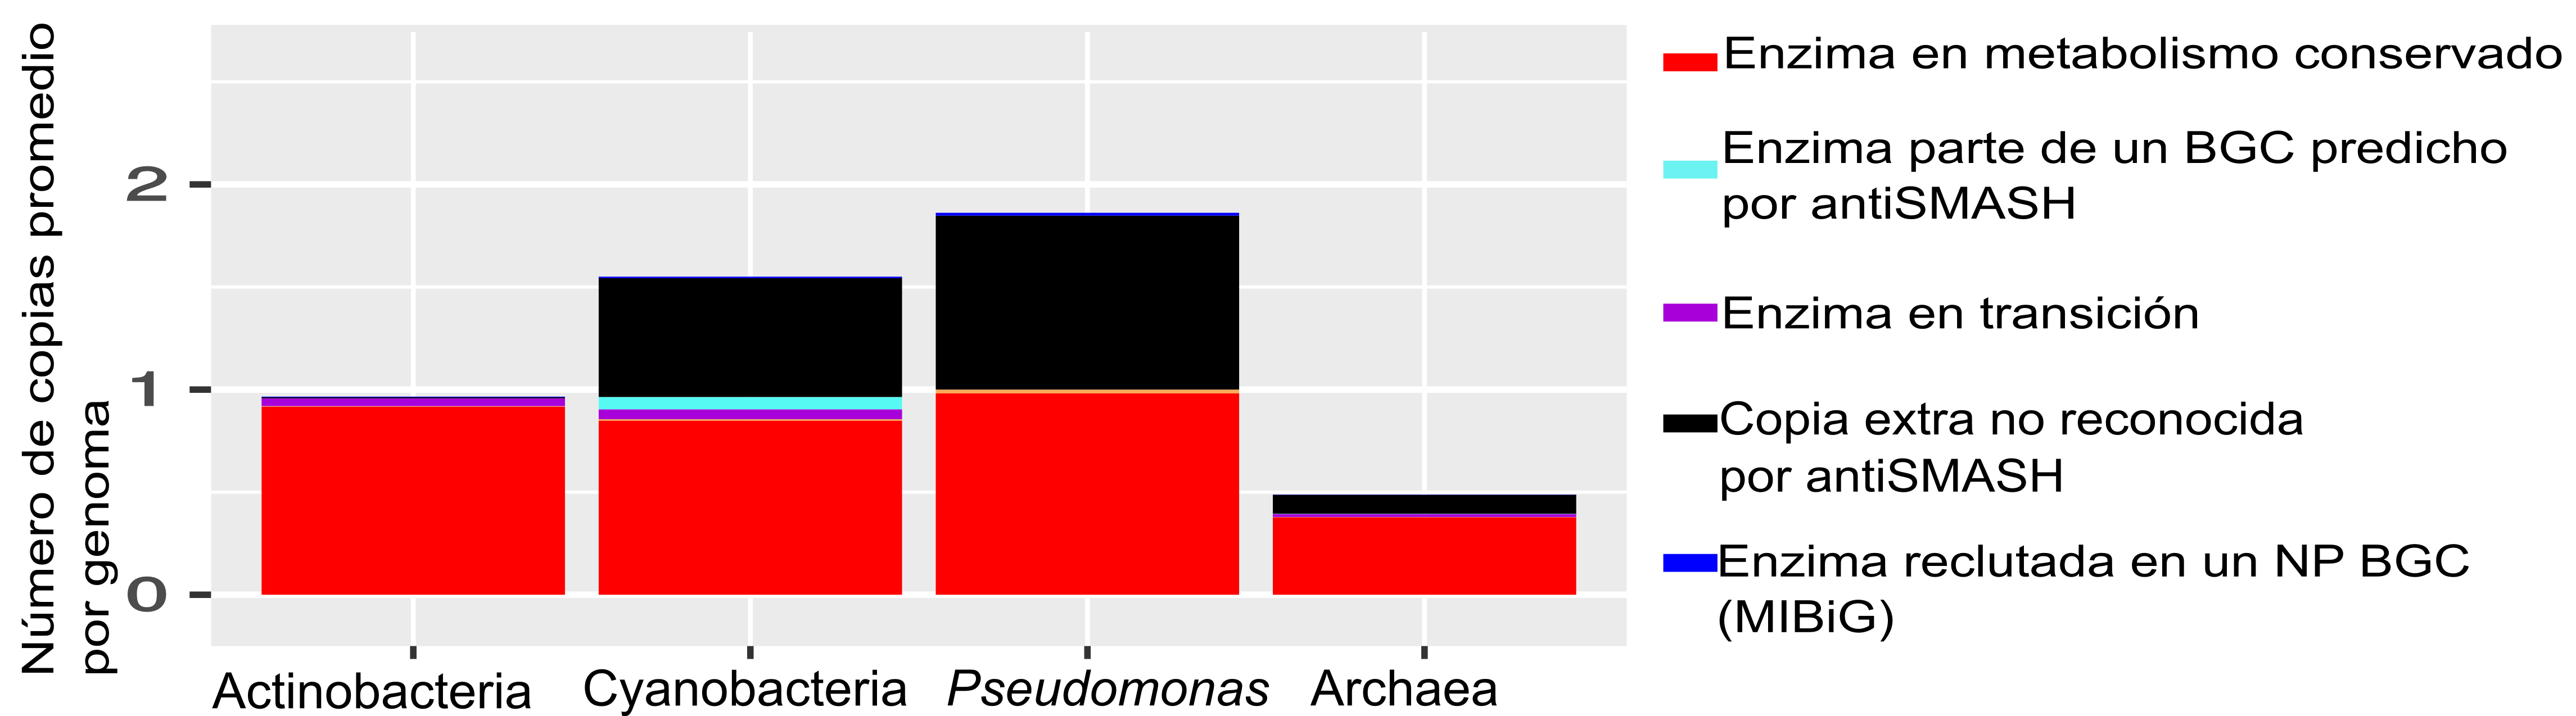
\includegraphics[angle = 0,scale = 0.8]{chapter4/PriAExpansiones.png}
  \caption[Expansiones de PriA en Actinobacteria, Cyanobacteria, Pseudomonas y Archaea]{\footnotesize{Número promedio de copias por genoma de PriA en Actinobacteria, Cyanobacteria, Pseudomonas y Archaea. Los colores muestran el destino metabólico asignado a cada copia según EvoMining. En rojo están los BBH a las enzimas semilla de metabolismo central. En morado las enzimas de metabolismo central también reconocidas por antiSMASH como parte de unBGC y en negro las copias sin un destino metabólico conocido.}}
  \label{fig:PriA_Expansiones}
  \end{figure}
  
  Después del conteo de número de copias promedio, se analizaron los
  árboles de PriA de EvoMining, tanto los coloreados de acuerdo al número
  de copias, \autoref{fig:PriAEvoMiningCopies}, como los coloreados según
  el destino metabólico, \autoref{fig:PriATrees}. En Actinobacteria la
  mayoría de las hojas son verdes reafirmando que existe sólo una copia
  por genoma en ese organismo. Sin embargo, existen varias hojas de color
  amarillo, indicando de dos copias en ese genoma. Las Actinobacterias con
  dos copias son \emph{Ornithinimicrobium pekingense} DSM 21552,
  \emph{Pseudonocardia} sp. P2, \emph{Serinicoccus marinus} DSM 15273,
  \emph{Serinicoccus profundi} MCCC 1A05965, \emph{Sphaerobacter
  thermophilus} DSM 20745 y \emph{Streptomyces} sp. CT34.
  
  En Cyanobacteria, \emph{Pseudomonas} y Archaea en contraste con
  Actinobacteria, se muestran una mezcla entre organismos que poseen una
  (verdes) o dos copias (amarillos) de PriA. Sin embargo al analizar
  detalladamente los árboles producidos por EvoMining en los distintos
  linajes, observamos que las copias extra tanto de Cyanobacteria como de
  \emph{Pseudomonas} son en realidad miembros de otras familias
  enzimáticas, que guardan cierta similitud de secuencia con PriA. En
  Cyanobacteria y \emph{Pseudomonas} la copia extra está en una rama
  divergente y muy poblada del árbol. En ambos casos esta segunda copia
  está en su mayoría anotada por RAST como imidazol glicerol fosfato
  sintasa ciclasa. En Archaea sin embargo, diversas especies de la clase
  Methanomicrobia sí tienen dos copias de PriA.
  
  \begin{figure}[h!tbp]
  \centering
  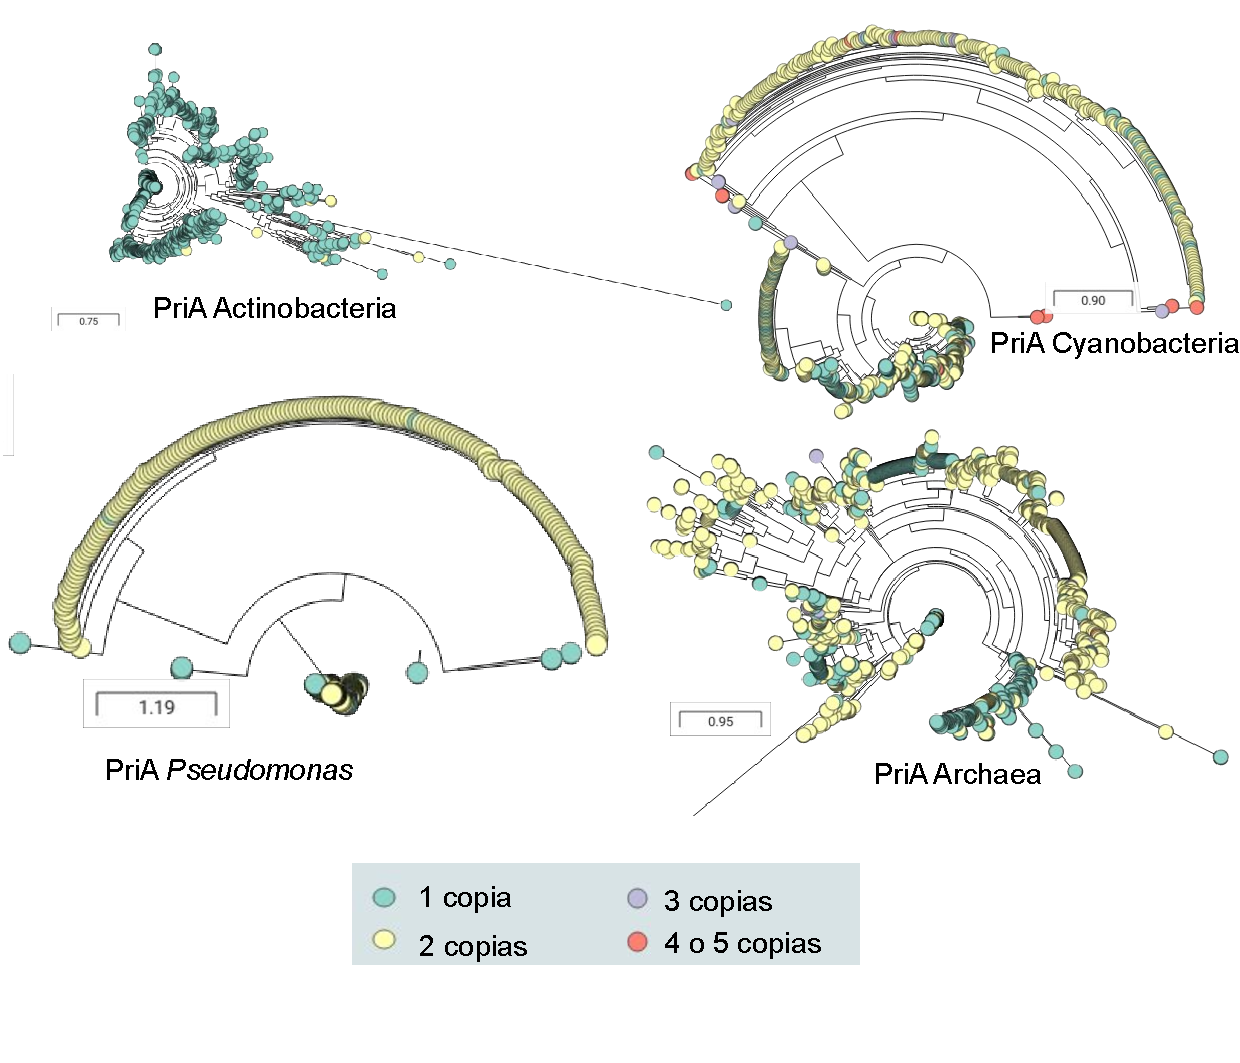
\includegraphics[angle = 0,scale = 0.8]{chapter4/PriAEvoMiningCopies.pdf}
  \caption[Copias extras de PriA en Actinobacteria, Cyanobacteria, Pseudomonas y Archaea]{\footnotesize{}}
  \label{fig:PriAEvoMiningCopies}
  \end{figure}
  
  Después de explorar cuáles organismos tienen expansiones de PriA, a
  continuación se muestra en la \autoref{fig:PriATrees} el posible destino
  metabólico de las copias extra de la familia. El árbl de Actinobacteria
  está poblado de hojas rojas, es decir de PriA dedicadas al metabolismo
  conservado, en este caso a las rutas de Histidina y Triptofano. Sin
  embargo hay algunas hojas grises, como es el caso de los dos
  \emph{Serenicoccus} mencionados previamente. Es posible que estas PriA
  puedan tener funciones alternativas. Además, en Actinobacteria la PriA
  de \emph{Janibacter Hoilley}, la rama más larga del árbol, es muy
  divergente. Esto se debe a que existe una fusión de PriA con HisH, que
  no parece ser un artefacto de anotación ya que hay otros
  \emph{Janibacter} con PriA ligeramente más grandes que el promedio.
  
  En Cyanobacteria hay pocas hojas verdes (EvoMining predictions) y no
  están localizadas cerca de la HisA de saxitoxin, el BGC proveniente de
  Cyanobacteria. En \emph{Pseudomonas} hay una gran población de
  predicciones de EvoMining, pero son falsos positivos, ya que estas no
  corresponden a una rama dedicada al metabolismo secundario, sino a la
  rama de la ciclasa. En Archaea algunas de los hojas grises, es decir sin
  destino metabólico conocido serán exploradas en la siguiente sección.
  
  \begin{figure}[h!tbp]
  \centering
  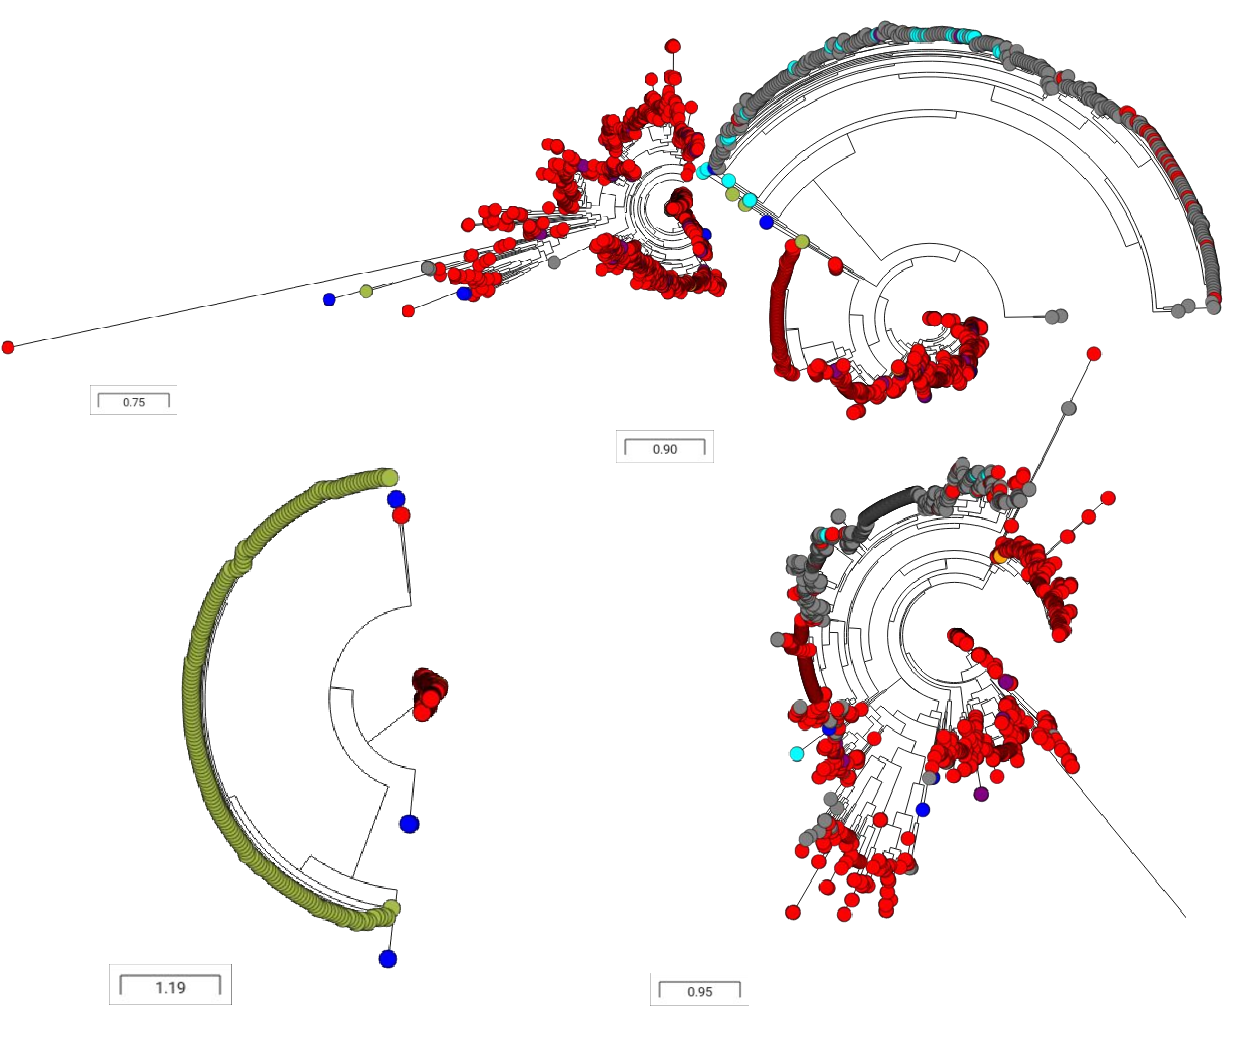
\includegraphics[angle = 0,scale = 0.8]{chapter4/PriAEvoMining.pdf}
  \caption[Árboles de destino metabólico de PriA en Actinobacteria, Cyanobacteria, {Pseudomonas} y Archaea según EvoMining]{\footnotesize{Árboles de destino metabólico de PriA en Actinobacteria, Cyanobacteria, {Pseudomonas} y Archaea según EvoMining}}
  \label{fig:PriATrees}
  \end{figure}
  
  Todos los reclutamientos (marcados en azul en el árbol) que tuvieron
  estas expansiones en estos linajes genómicos están listados en la tabla
  \autoref{tab:reclutamientos}. Entre ellos se encuentran dos toxinas de
  Cyanobacteria{[}\protect\hyperlink{ref-moustafa_origin_2009}{103}{]}, un
  lipopolisacárido producido por una Proteobacteria y un BGC productor de
  cloro pentostatina producido en Actinobacteria
  {[}\protect\hyperlink{ref-gao_biosynthesis_2017}{167}{]}.
  
  \begin{longtable}[]{@{}lccclll@{}}
  \caption{Reclutamientos de expansiones de PriA en MIBiG
  \label{tab:reclutamientos}}\tabularnewline
  \toprule
  Compuesto & Actinobacteria & Cyanobacteria & Pseudomonas & Archaea & BGC
  origen & Clase\tabularnewline
  \midrule
  \endfirsthead
  \toprule
  Compuesto & Actinobacteria & Cyanobacteria & Pseudomonas & Archaea & BGC
  origen & Clase\tabularnewline
  \midrule
  \endhead
  \href{http://mibig.secondarymetabolites.org/repository/BGC0000188/index.html\#cluster-1}{saxitoxin}
  & x & x & x & x & Cyanobacteria & Alcaloide\tabularnewline
  \href{http://mibig.secondarymetabolites.org/repository/BGC0000775/index.html\#cluster-1}{lipopolisacárido}
  & x & x & x & x & Proteobacteria & Sacarido\tabularnewline
  \href{http://mibig.secondarymetabolites.org/repository/BGC0000928/index.html\#cluster-1}{toxin}
  & x & x & x & x & Cyanobacteria & Otros\tabularnewline
  \href{http://mibig.secondarymetabolites.org/repository/BGC0001484/index.html\#cluster-1}{ada}
  & x & x & x & x & Actinobacteria & Otros\tabularnewline
  \bottomrule
  \end{longtable}
  
  La pentostatina es un atibiótico nucleosídico derivado de adenosina,
  cuyo cluster es llamado \emph{ada} . La PriA del cluster \emph{ada} es
  llamada \emph{adaK} y sí parece participar del cluster, ya que muestra
  una isomerización sobre un sustrato similar a los nativos de PriA,
  \autoref{fig:ada}, con un anillo de 5 carbonos, dos OH, un oxígeno y un
  grupo fosfato . Esta isomerización es muy parecida a la que realiza PriA
  sobre ProFAR y PRA. Esta PriA no es una copia extra, sino la copia única
  de este organismo. Este contexto genómico no se encuentra conservado en
  las copias vecinas en el árbol. Es relevante mencionar que la mutante de
  PriA no suprime la producción de este antibiótico en \emph{Actinomadura}
  sp. ATCC 39365, por lo que los autores especulan que otra enzima podría
  estar realizando la isomerización redundantemente. \emph{Actinomadura}
  no posee una copia de TrpF que sería el candidato inmediato.
  
  \begin{figure}[h!tbp]
  \centering
  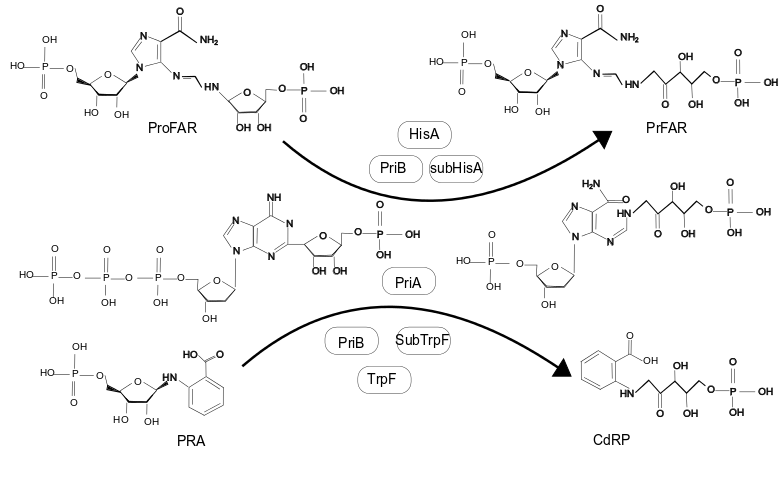
\includegraphics[angle = 0,scale = 0.6]{chapter4/ada.png}
  \caption[PriA participa en la síntesis del antibiótico {ada} en {Actinomadura} ]{\footnotesize{PriA participa en la síntesis del antibiótico {ada} en {Actinomadura}. Los sustratos nativos de Pria, ProFAR y PRA son isomerizados de manera muy similar a un paso en la ruta de síntesis de {ada} }}
  \label{fig:ada}
  \end{figure}
  
  Finalmente, los árboles que se produjeron por EvoMining están
  disponibles para exploración interactiva en Microreact en los links de
  la \autoref{tab:arboles}:
  
  \begin{longtable}[]{@{}lc@{}}
  \caption{Árboles EvoMining de PriA en MicroReact
  \label{tab:arboles}}\tabularnewline
  \toprule
  Linaje & Link al árbol de EvoMining en Microreact\tabularnewline
  \midrule
  \endfirsthead
  \toprule
  Linaje & Link al árbol de EvoMining en Microreact\tabularnewline
  \midrule
  \endhead
  Actinobacteria &
  \href{https://microreact.org/project/7g2IGfkv9}{7g2IGfkv9}\tabularnewline
  Cyanobacteria &
  \href{https://microreact.org/project/qF6jWRMox}{qF6jWRMox}\tabularnewline
  \emph{Pseudomonas} &
  \href{https://microreact.org/project/ydff6DWqs}{ydff6DWqs}\tabularnewline
  Archaea &
  \href{https://microreact.org/project/Ig-m9Cm6f}{Ig-m9Cm6f}\tabularnewline
  \bottomrule
  \end{longtable}
  
  \subsection{Análisis de contextos genómicos de PriA en distintos linajes
  utilizando
  CORASON}\label{analisis-de-contextos-genomicos-de-pria-en-distintos-linajes-utilizando-corason}
  
  En Actinobacteria, se observó que todos los \emph{Streptomyces} tienen
  el cluster de PriA parcialmente conservado con respecto al BGC de
  \emph{Streptomyces coelicolor}. Ejemplos de ello son \emph{S. roseous},
  \emph{S. sviceus}, \emph{S. sp C} y \emph{S. Mg1} donde genes tanto de
  la ruta de histidina como de triptofano rodean a PriA. Otros como
  \emph{S rimosus} , \emph{S HmicA12} y \emph{S. sp CT34} tienen los genes
  de triptofano más alejados \autoref{fig:PriACORASON} . Como ya se
  describió en la sección de EvoMining, el único organismo de este género
  con una copia extra de PriA es \emph{Streptomyces} CT34. Esta copia
  parece deberse a transferencia horizontal dado que su mejor hit en NCBI
  proviene de una \emph{Lentzea}. Aún así parece ser un homólogo lejano ya
  que tuvo 50\% de identidad en 98\% de cobertura con respecto a la copia
  de \emph{Lentzea}. Otro caso interesante en Actinobacteria son las
  Actinomaduras, ya que CORASON muestra que el cluster \emph{ada} no está
  conservado en ellas (datos no mostrados). Además, también en
  Actinobacteria CORASON muestra en \emph{Sporichthya polymorpha} DSM
  43042 una PriA precedida por una NRPS, una enzima por excelencia de
  productos naturales. En otros organismos antiSMASH predice que PriA
  forma parte de clusters putativos, por ejemplo en \emph{Modestobacter
  marinus} NC\_0179551, \emph{Geodermatophilus obscurus}, y en
  \emph{Streptacidiphilus jeojiense}. Los contornos de los genes
  reconocidos por antiSMASH como parte de un BGC son marcados en azul en
  las figuras de CORASON.
  
  En cuanto a Archaea, los contextos mostrados en los páneles b y c de la
  \autoref{fig:PriACORASON} muestran que si bien existen algunos contextos
  como el de ciertos \emph{Thermococcus} donde PriA está rodeada de genes
  de histidina y triptofano, esta configuración no es la generalidad. Al
  contrario, parece que no hay una configuración conservada que prevalezca
  en todo Archaea. Esto puede deberse a que Archaea es un dominio, no un
  phylum como Actinobacteria, y por tanto hay una mayor distancia entre
  los organismos que la conforman.
  
  \begin{figure}[h!tbp]
  \centering
  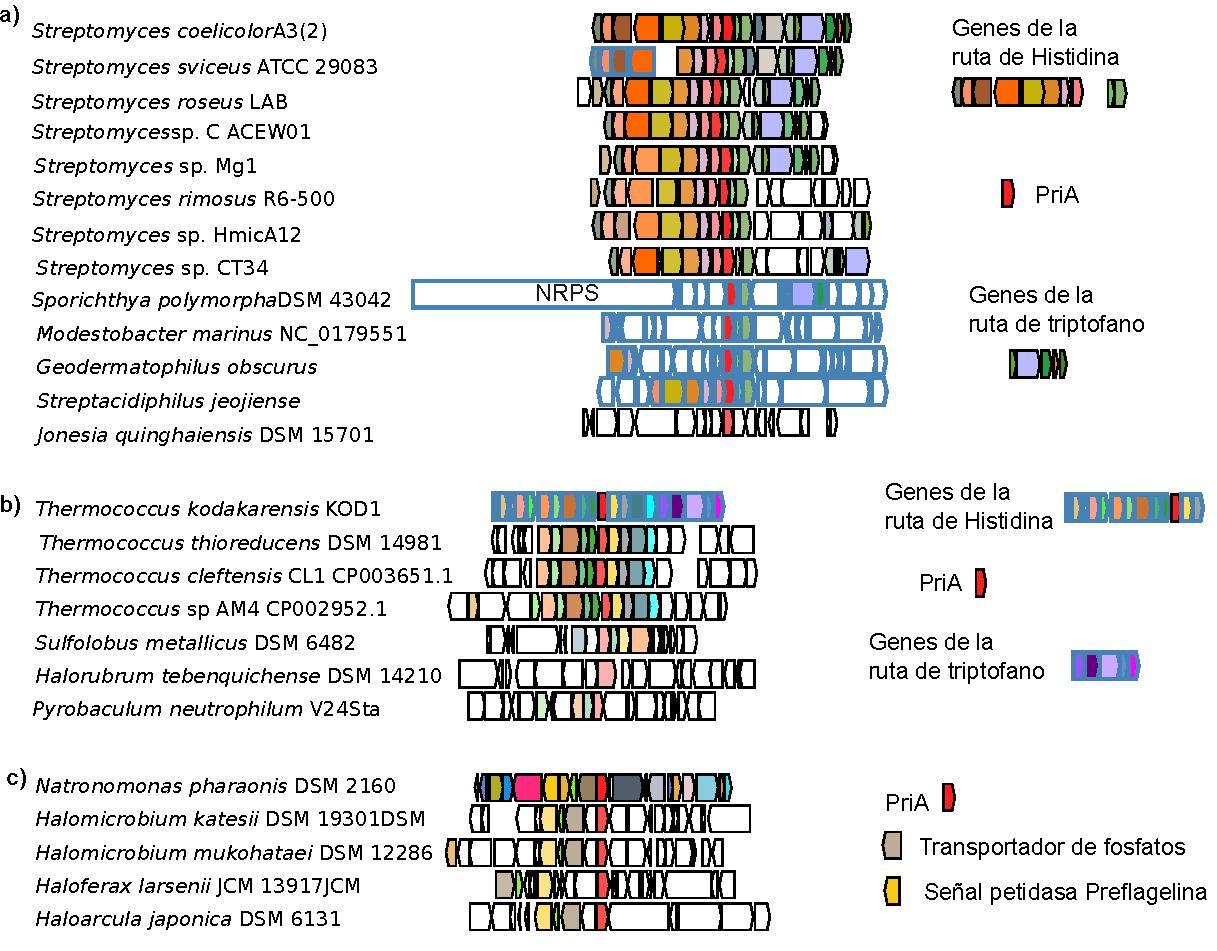
\includegraphics[angle = 0,scale = 0.7]{chapter4/CORASON/CORASON.pdf}
  \caption[Contextos de PriA en Actinobacteria y Archaea]{\footnotesize{Contextos de PriA en Actinobacteria y Archaea}}
  \label{fig:PriACORASON}
  \end{figure}
  
  En cuanto a PriA en Cyanobacteria la visualización de contextos
  producida por CORASON tomando como referencia el cluster de saxitoxin,
  muestra que las enzimas biosintéticas de ese no están conservadas en
  otros organismos. Además en el lado izquierdo de la
  \autoref{fig:saxitoxin} se muestra que la PriA del BGC saxitoxin no está
  ubicada en una rama de PriA divergente, al contrario está en la parte
  más conservada. Por estas razones es posible que PriA esté en la orilla
  del BGC de saxitosin y más bien no participe en la síntesis de este
  compuesto.
  
  \begin{figure}[h!tbp]
  \centering
  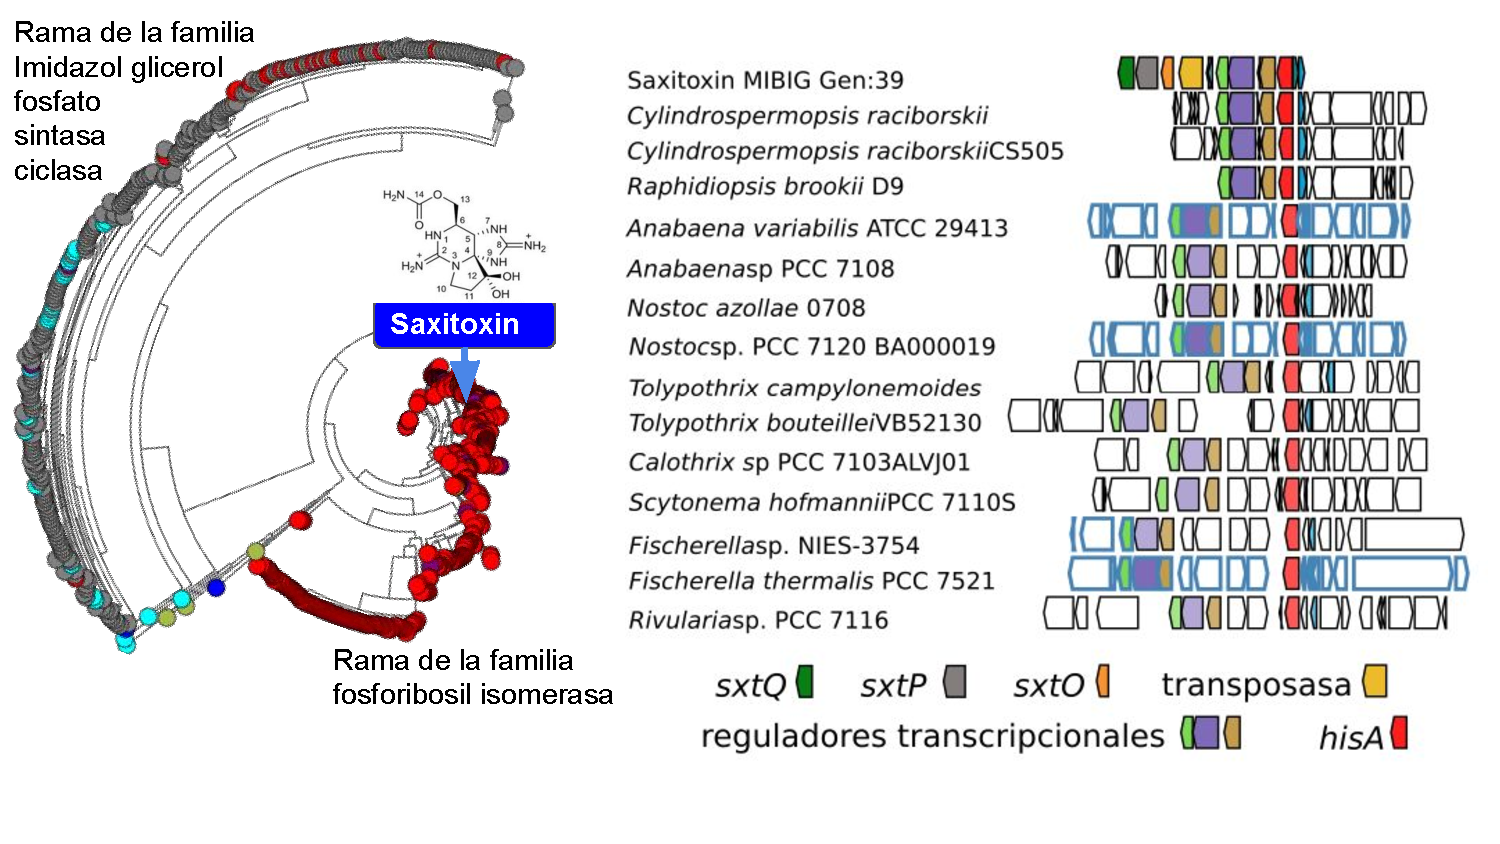
\includegraphics[angle = 0,scale = 0.7]{chapter4/CORASON/saxitoxin.pdf}
  \caption[HisA en saxitoxin, un cluster de Cyanobacteria ]{\footnotesize{HisA en saxitoxin, un cluster de Cyanobacteria }}
  \label{fig:saxitoxin}
  \end{figure}
  
  \section{El monitoreo en cambios de aminoácidos en PriA para estudiar
  rutas evolutivas y reconstrucciones de la estructura
  tridimensional.}\label{el-monitoreo-en-cambios-de-aminoacidos-en-pria-para-estudiar-rutas-evolutivas-y-reconstrucciones-de-la-estructura-tridimensional.}
  
  En esta segunda sección concerniente a la familia PriA se busca
  información contenida en la secuencia de aminoácidos. En la primera
  parte se discute cómo en datos de evolución dirigida en el laboatorio no
  se encontró ninguna trayectoria en donde algún paso incrementara la
  actividad de PriA en sus dos sustratos nativos. En la segunda parte se
  muestra una reconstrucción de la estructura tridimensional de PriA
  basada en la covarianza de sus aminoácidos en secuencias del registro
  evolutivo.
  
  \subsection{Al transformar una subHisA en una PriA mediante mutaciones
  no se observó ninguna trayectoria creciente para ambos sustratos
  (darwiniana)}\label{al-transformar-una-subhisa-en-una-pria-mediante-mutaciones-no-se-observo-ninguna-trayectoria-creciente-para-ambos-sustratos-darwiniana}
  
  En esta sección analizamos cómo cambia la capacidad catalítica de PriA
  sobre un sustrato mientras se varía la del otro. Para ello se utilizaron
  datos de mutantes de subHisA de \emph{Corynebacterium diphteriae}. Estas
  mediciones de cinéticas enzimáticas fueron obtenidos del trabajo de
  tesis de Lianet Noda {[}\protect\hyperlink{ref-noda_tesis_2012}{71}{]}.
  A partir de la secuencia original que se mostró es una subHisA, se
  realizaron mutantes con el objetivo de alcanzar la promiscuidad, es
  decir de convertir la enzima subHisA en una PriA. Se comenzó con
  diferentes mutantes puntuales adicionando una mutación cada vez, hasta
  llegar a una con 11 mutaciones. En esta colección de mutantes varias
  ganaron la función de PRA isomerasa, a distintos niveles. La que alcanzó
  mayor actividad PRA isomerasa fue la \(9.3\), una variante con nueve
  mutaciones. En estos datos quedaba pendiente la exploración de las
  rutas, es decir cómo es el camino desde una mutante sencilla hasta una
  múltiple ¿cuántas rutas son posibles? ¿Existe alguna tendencia en
  ciertos momentos de la ruta sobre el incremento/decremento de alguna de
  las dos funciones?
  
  Asi pues se desarrolló un
  \href{https://github.com/nselem/perlas/tree/master/LiaTrayectory}{script}
  utilizando recursividad para reconstruir todas las rutas posibles. El
  total de rutas calculadas hasta la mutación 11 fue de 2928 caminos, las
  rutas posibles hasta la mutante 9.3 son 790. Estas rutas son mostradas
  en la \autoref{fig:PriARutas}.
  
  \begin{figure}[h!tbp]
  \centering
  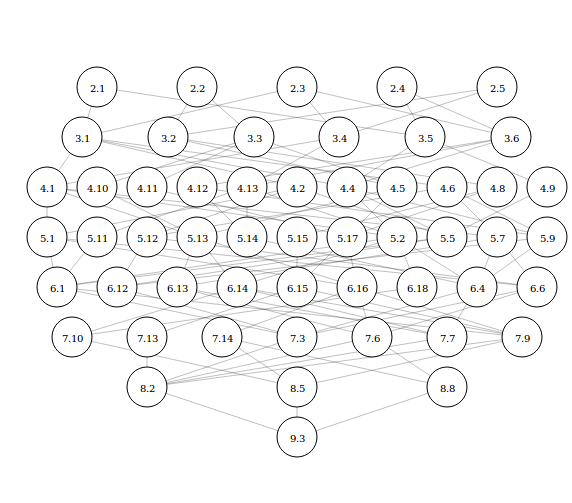
\includegraphics[angle = 0,scale = 0.6]{conclusion/Solocirculos.png}
  \caption[Rutas desde una subHisA hasta una variante con 9 mutaciones]{\footnotesize{Rutas desde una subHisA hasta una variante con 9 mutaciones. En cada círculo el primer dígito indica el número de mutaciones}}
  \label{fig:PriARutas}
  \end{figure}
  
  Al analizar los cambios sufridos en cada actividad en cada paso de cada
  ruta se descubrió que no existe en ellas una trayectoria no decreciente
  para ningún sustratos. Como ejemplo, en la \autoref{fig:PriARutas} se
  muestran las rutas donde cada mutante mantiene un nível mínimo de
  actividad de ProFAR isomerasa
  (\(\frac{K_{cat}}{K_m} PriA_{ProFAR} \ge .004\)). En azul sólido se ven
  los incrementos en PRA y en rojo sólido los incrementos en ProFAR. Las
  líneas punteadas indican que la actividad decreció en ese paso de la
  ruta. Entre una y cuatro mutaciones el azul sólido es predominante, es
  decir se incrementa la actividad para PRA, pero entre 4 y 5 mutaciones
  ningún paso incrementa la actividad de PRA y en cambio sí se incrementa
  la actividad para ProFAR, esta figura sugiere que al mejorar una
  actividad se compromete el mejoramiento de la otra. En este ejemplo, las
  mutaciones puntuales que llevan a una enzima monofuncional a adquirir
  promiscuidad no mantienen una tendencia no decreciente de principio a
  fin sobre ninguna ruta en ninguna de las dos reacciones isomerización de
  PRA e isomerización de ProFAR. Este tipo de trayectorias se conoce como
  no darwininana ya que siempre existe algún paso donde decrece alguna de
  las actividades.
  
  \begin{figure}[h!tbp]
  \centering
  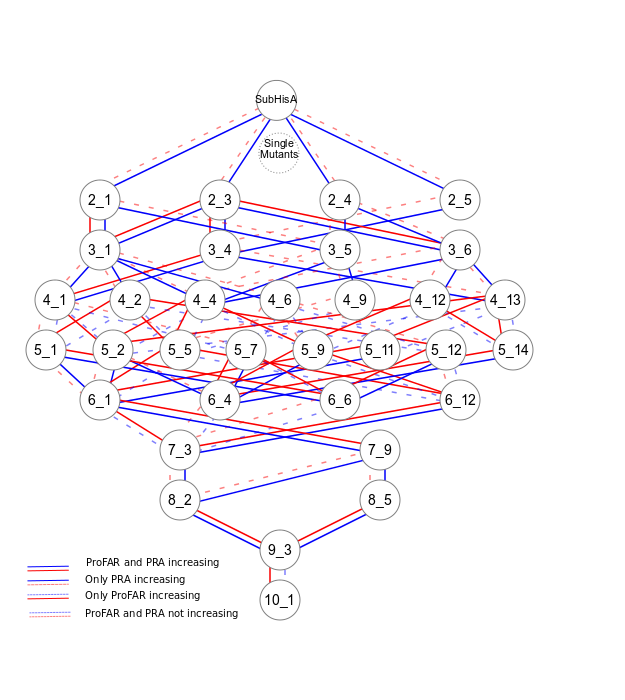
\includegraphics[angle = 0,scale = 0.8]{chapter4/LianetFiguras/SolocirculosPRA_PRO_RUTAS_10_1_r002.png}
  \caption[Positive increments on PRA]{\footnotesize{Rutas de evolución dirigida para ganar la función PRA. En la figura se muestra como la mayoría de los pasos que incrementan una función hacer decrecer la capacidad catalítica de la otra. }}
  \label{fig:PRARutas}
  \end{figure}
  
  \subsection{Los residuos que covarían en el registro evolutivo de PriA
  permiten una reconstrucción aproximada de su estructura
  tridimensional}\label{los-residuos-que-covarian-en-el-registro-evolutivo-de-pria-permiten-una-reconstruccion-aproximada-de-su-estructura-tridimensional}
  
  El estudio de la evolución de PriA en la sección anterior nos
  proporcionó el aprendizaje de que para adquirir una actividad el camino
  no es estrictamente creciente. En cambio, suele haber pasos donde alguna
  de las dos actividades baja. En esta sección utilizaremos el registro
  evolutivo resultado de millones de años, tomaremos miles de homólogos de
  PriA para inferir la estructura tridimensional de una secuencia.
  Evcouplings es un método que considera las secuencias génicas existentes
  como experimentos exitosos de la naturaleza. Con esta información
  obtiene la covariación entre pares de aminoácidos de las secuencias
  existentes en el registro evolutivo. Los pares fuertemente relacionados
  se denominan acoplamientos, estos acoplamientos a menudo están cerca
  físicamente en la estructura terciaria de la proteína. Se ha demostrado
  que muchas proteínas contienen suficientes acoplamientos distribuidos
  ampliamente en toda la secuencia, de forma que con ellos es posible la
  reconstrucción de su estructura tridimensional
  {[}\protect\hyperlink{ref-marks_protein_2011}{168}{]}. En esta sección
  se aplicará EVcouplings para reconstruir la estructura tridimensional de
  PriA.
  
  Las diferencias a nivel estructural pueden amplificar la información
  proporcionada por variaciones a nivel de secuencia. Por este motivo se
  decidió implementar Evcouplings
  {[}\protect\hyperlink{ref-marks_protein_2011}{168}{]}, para poder
  aplicarlo a la familia PriA. Este método es de difícil instalación ya
  que tiene muchas dependencias, por ello desarrollé un contenedor docker
  donde las dependencias y el software quedan instalados. Este desarrollo
  fue incluido por los desarrolladores originales como sugerencia de
  instalación.\\
  El contenedor docker implementa EVcouplings python framework
  {[}\protect\hyperlink{ref-hopf_evcouplings_2019}{169}{]} que comprende
  cinco etapas para estudiar el análisis de coevolución de residuos de una
  familia de proteínas. Estas etapas son i) Alineado, ii) análisis de
  acoplamiento, iii) plegamiento basado en acoplamientos iv) análisis de
  mutación y v) comparación con estructuras conocidas.
  
  EVcouplings fue aplicado a PriA de Streptomyces coelicolor con
  identificador de Uniprot HIS4\_STRCO. Las secuencias para las
  alineaciones se recuperaron automáticamente de Uniprot, otros parámetros
  se dejaron con la configuración inicial del archivo de configuración.
  Como resultado se modeló la estructura de PriA con los acoplamientos de
  sus aminoácidos. Una comparación con una estructura cristalográfica es
  mostrada en la \autoref{fig:CouplingsFoldingPriA}
  
  La estructura reconstruida es parecida, pero para obtener mejor
  definición es posible que se deba refinar la selección de las secuencias
  del alineamiento, diferenciando entre secuencias conocidas de PriA,
  subHisA, PriB y subTrpF.
  
  \begin{figure}[h!tbp]
  \centering
  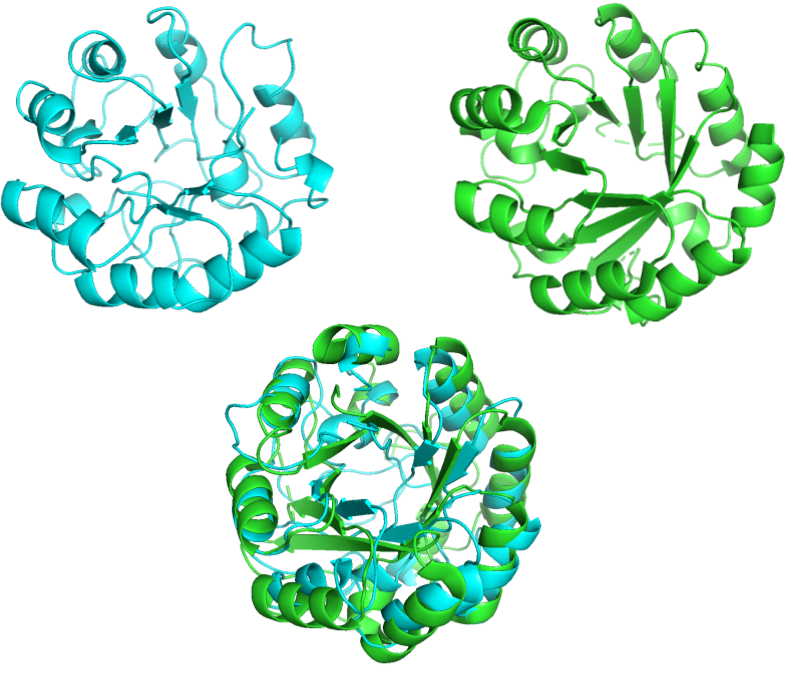
\includegraphics[angle = 0,scale = .5]{chapter4/Couplings/PriACouplingFoldings.png}
  \caption[Superposición de estructura de PriA generado por Folding con la estructura cristalográfica]{\footnotesize{Comparación de estructura de PriA de {Streptomyces} {coelicolor} generada por EVcouplings con la estructura cristalográfica}}
  \label{fig:CouplingsFoldingPriA}
  \end{figure}
  
  Finalmente los aminoácidos utilizados en la evolución dirigida de la
  sección anterior fueron comparados con los provistos por EVCouplings
  como altamente partícipes en la covariación. Los 10 con más
  acoplamientos fueron 90L, 117V, 127V, 48W, 208I, 87D, 135T, 21V, 109E.
  Sólo el 21V es parte los aminoácidos mutados en el estudio previament
  descrito. En la \autoref{tab:aminoacidos} se muestra en la primera
  columna los aminoácidos variados en el estudio de mutación dirigida en
  \emph{Corynebacterium}, en la segunda columna el aminoácido
  correspondiente en la secuencia de \emph{Streptomyces coelicolor} y
  finalmente su correspondiente acoplamiento más significativo.\\
  
  \begin{longtable}[]{@{}ccc@{}}
  \caption{Árboles EvoMining de PriA en MicroReact
  \label{tab:aminoacidos}}\tabularnewline
  \toprule
  \emph{Corynebacterium} & \emph{Streptomyces} & Acoplamiento más
  relevante\tabularnewline
  \midrule
  \endfirsthead
  \toprule
  \emph{Corynebacterium} & \emph{Streptomyces} & Acoplamiento más
  relevante\tabularnewline
  \midrule
  \endhead
  D20V & 21V & 173T\tabularnewline
  L48I & 49L & 76I\tabularnewline
  F50L & 51L & 70V\tabularnewline
  M66I & 67I & 80L\tabularnewline
  T80S & 81S & 102N\tabularnewline
  A97C & 98C & 107A\tabularnewline
  D127A & 128G & 164V\tabularnewline
  A129D & 130D & 168I\tabularnewline
  T139L & 136L & 151T\tabularnewline
  Y214L & 211Y & -\tabularnewline
  E230A & 227A & 234E\tabularnewline
  \bottomrule
  \end{longtable}
  
  Una forma gráfica de ver esta tabla es la \autoref{fig:couplings}. En
  las líneas naranjas se muestra como el aminoácido 21D tiene un
  acoplamiento con el 173T, que está muy cerca del 175D que ha sido
  asociado con la actividad de isomerización de PRA, pero no de ProFAR.
  
  \begin{figure}[h!tbp]
  \centering
  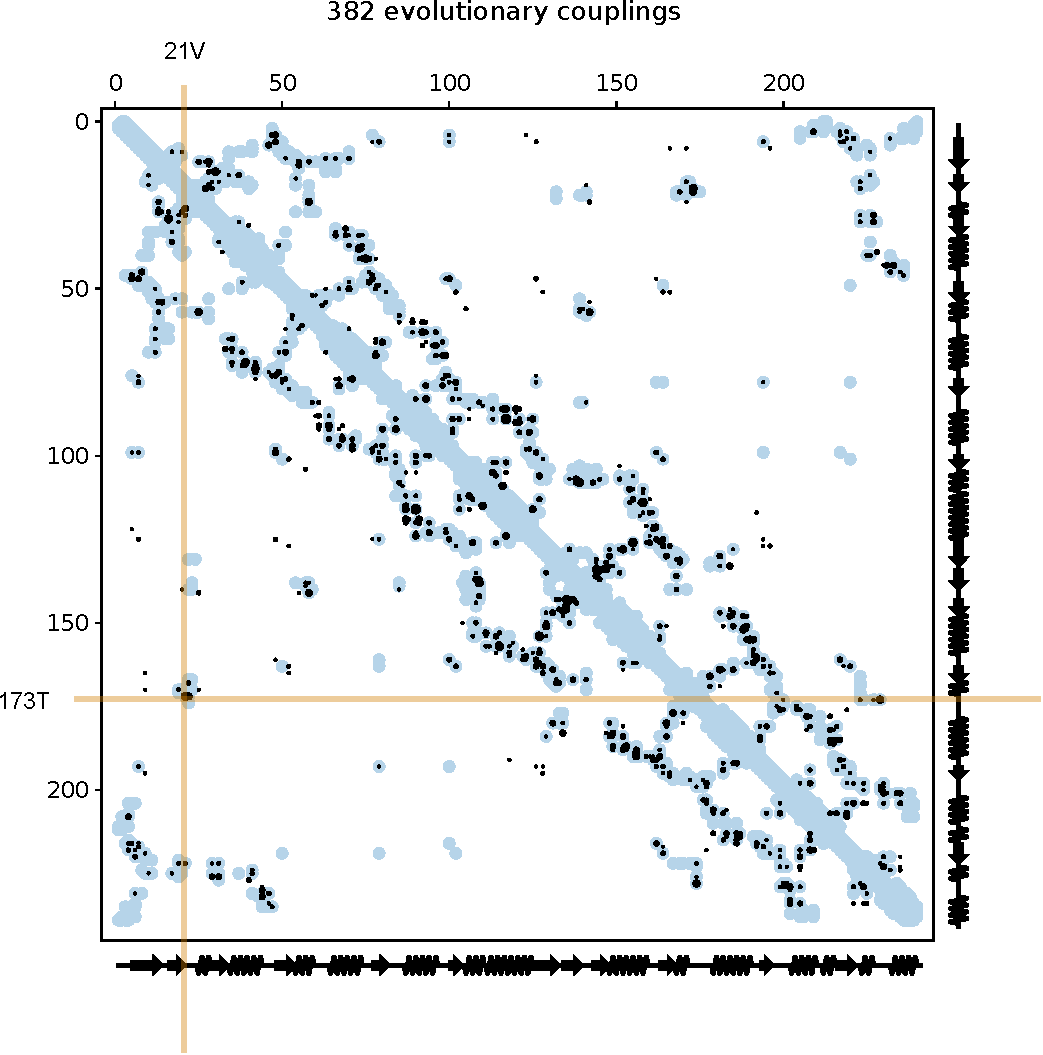
\includegraphics[angle = 0,scale = .5]{chapter4/Couplings/HIS4_STRCO_1-200/align/couplings.pdf}
  \caption[Visualización de los acoplamientos en la familia PriA]{\footnotesize{Visualización de los acoplamientos en la familia PriA}}
  \label{fig:couplings}
  \end{figure}
  
  Además se investigaron los aminoácidos catalíticos D130
  {[}\protect\hyperlink{ref-due_bisubstrate_2011}{170}{]} y D175
  reportados en \emph{Mycobacterium
  tuberculosis}{[}\protect\hyperlink{ref-verduzco-castro_co-occurrence_2016}{67}{]}
  que corresponden a en \emph{S coelicolor} D11, D131 y D171. Se econtró
  que existe un conjunto de secuencias donde estos residuos no están
  presentes \autoref{fig:Alineamiento}. La mayoría de estassecuencias es
  fuera del phylum Actinobacteria, como PSeudomonas, Cyanobacteria,
  Enterobacteria, Proteobacteria y Chloroflexi. Sin embargo,
  interesantemente se encontraron 159 Corynebacterium, 49 Streptomyces y 2
  Actinokineospora sin 131D, entre ellos el ya mencionado
  \emph{Streptomyces CT 34} y \emph{Streptomyces rimosus} . En
  Corynebacterium se encuentra localizada la familia subHisA y en
  Streptomyces la familia PriB, la variabilidad mostrada en estos géneros
  podría estar relacionada con la existencia de estas familias. A futuro,
  para obtener resultados exclusivos sobre la covariación de residuos en
  Actinobacteria, se debe proveer un alineamiento exclusivo de
  Actinobacteria.
  
  \begin{figure}[h!tbp]
  \centering
  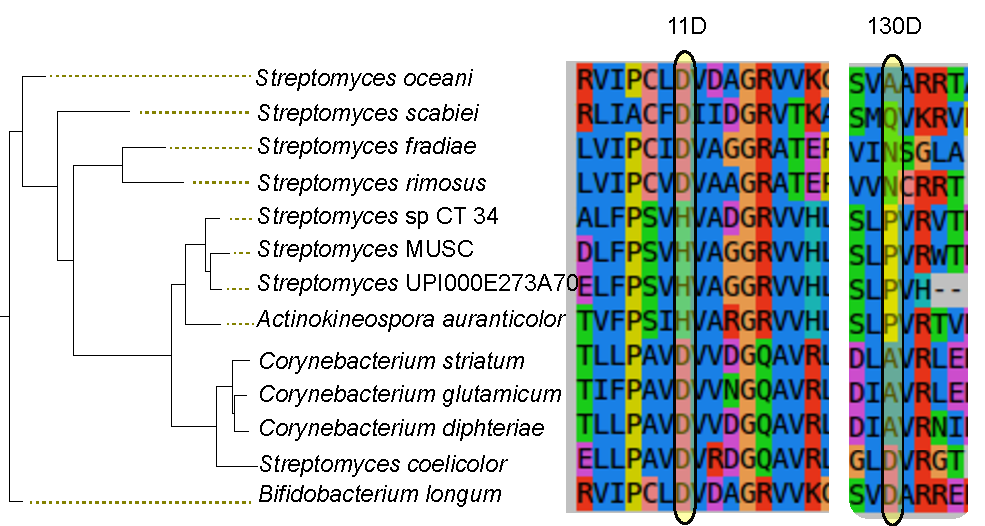
\includegraphics[angle = 0,scale = .5]{chapter4/Couplings/HIS4_STRCO_1-200/align/alineamiento.pdf}
  \caption[Miembros de PriA que poseen variantes los residuos catalíticos D11, D130]{\footnotesize{Miembros de PriA que poseen variantes los residuos catalíticos D11, D130}}
  \label{fig:Alineamiento}
  \end{figure}
  
  Finalmente la predicción del efecto de una mutacion para cada posición
  de la secuencia para cada aminoacido podemos verlo en la siguiente
  \autoref{fig:CouplingsMutationsPriA}
  
  \begin{figure}[h!tbp]
  \centering
  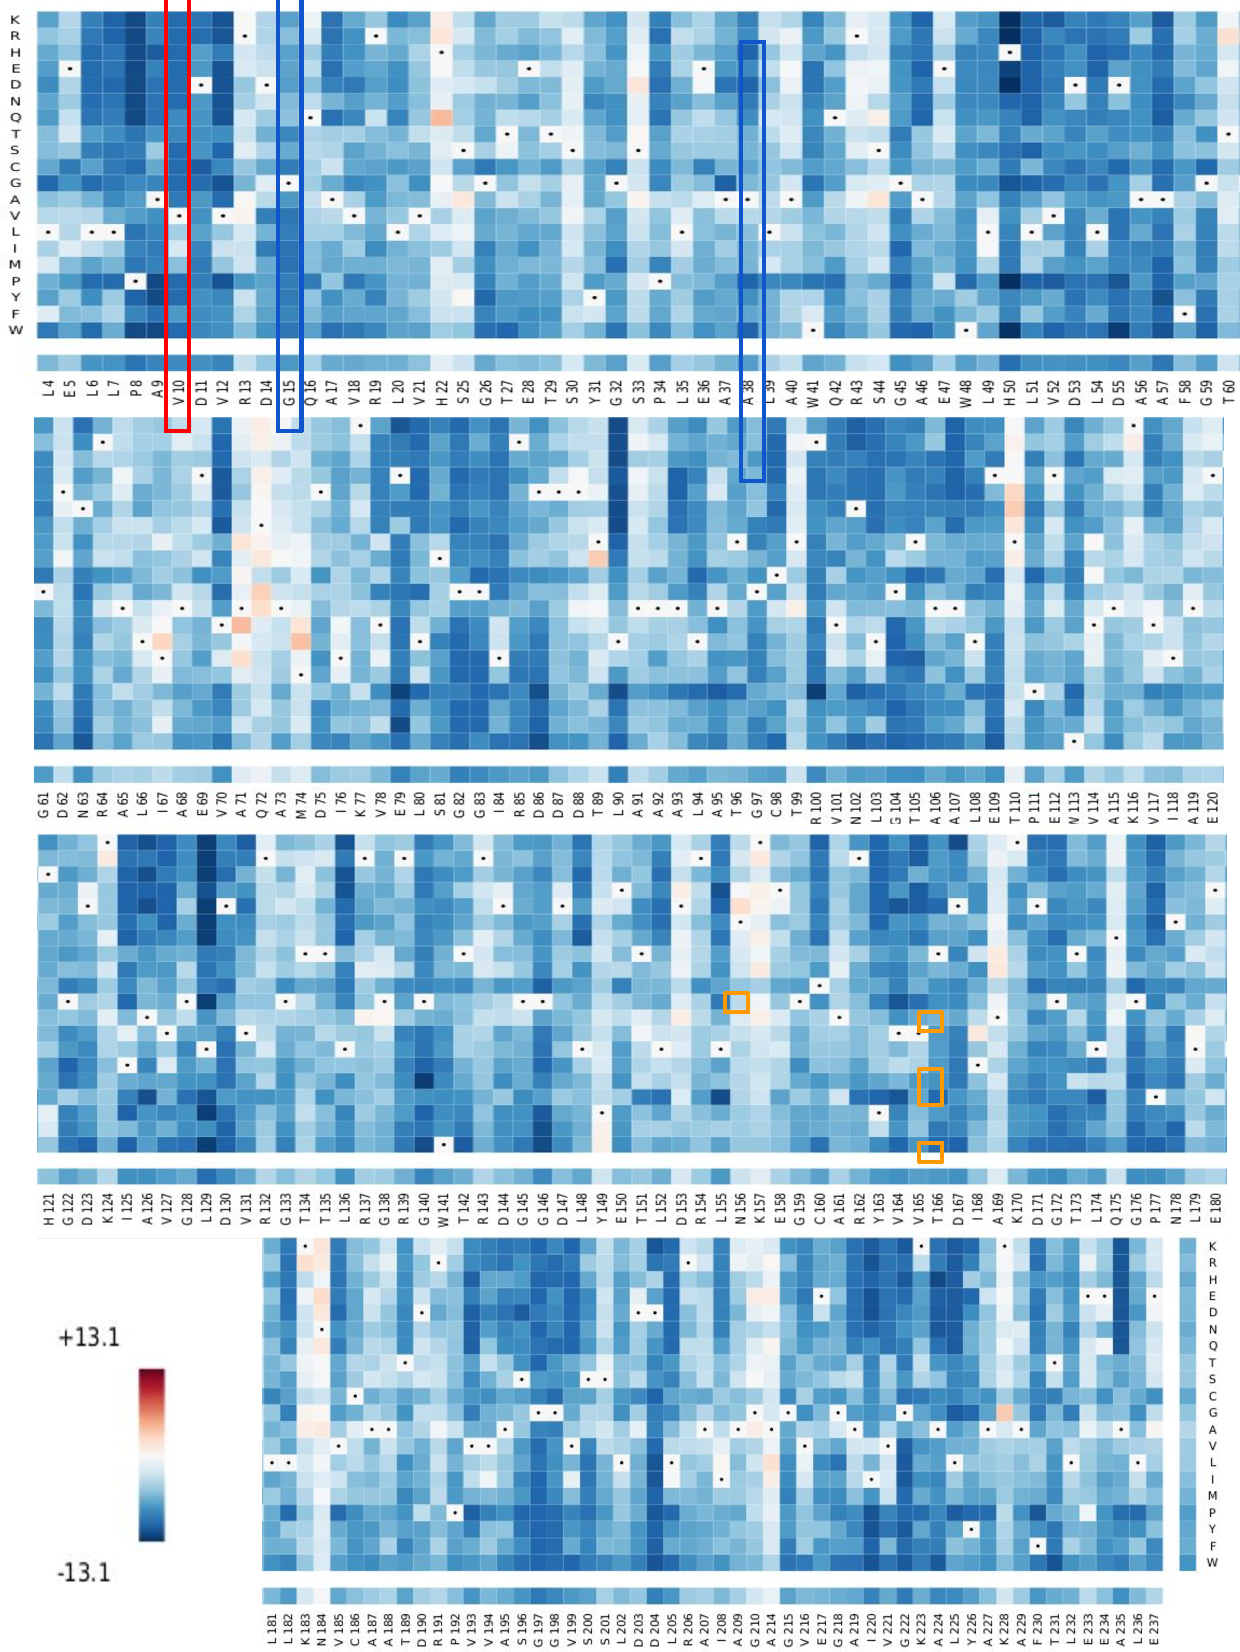
\includegraphics[angle = 0,scale = .8]{chapter4/Couplings/PriAMutations.pdf}
  \caption[Tendencia de mutaciones observada en secuencias de PriA]{\footnotesize{}}
  \label{fig:CouplingsMutationsPriA}
  \end{figure}
  
  \section{Afinidad de enzimas selectas por sustratos químicamente
  parecidos a PRA y
  PROFAR}\label{afinidad-de-enzimas-selectas-por-sustratos-quimicamente-parecidos-a-pra-y-profar}
  
  Además de los sustratos conocidos ProFAR y PRA en los que PriA es capaz
  de realizar una isomerización, es posible que PriA pueda ser promiscua
  en otros sustratos. De hecho como se vio en la sección de EvoMining de
  este capítulo, PriA parece participar en la síntesis del antibiótico
  pentostaina \emph{ada}. Tomando este ejemplo como inspiración, se
  colectaron en la literatura sustratos químicamente parecidos a ProFAR y
  PRA \autoref{fig:Eschema1},
  \autoref{fig:Eschema2},\autoref{fig:Eschema3},\autoref{fig:Eschema4}.
  Así pues, esta sección buscará mostrar sustratos parecidos a los nativos
  de PriA para posteriormente probar alguno en copias selectas de PriA
  provenientes de diversos organismos.
  
  Se seleccionaron veinte sustratos para realizar docking entre ellos y
  las estructuras de las secuencias de PriA S1, S2, \ldots{} S20 sustratos
  fueron recolectados de la literatura y las predicciones de la
  quimioinformática. S3 PRA y S7 PROFAR son sustratos nativos, S13-S16 son
  sustratos activados por la luz, S17 PRAP, S18 Compuesto V, se
  encontraron en la literatura, S6 GMP, S11 GTP y otros fueron sugeridos
  por chemioinformatics. Para tener una diea de la diversidad de estos
  sustratos, se realizó entre ellos, un cálculo de distancias de Tanimoto.
  
  \begin{figure}[h!tbp]
  \centering
  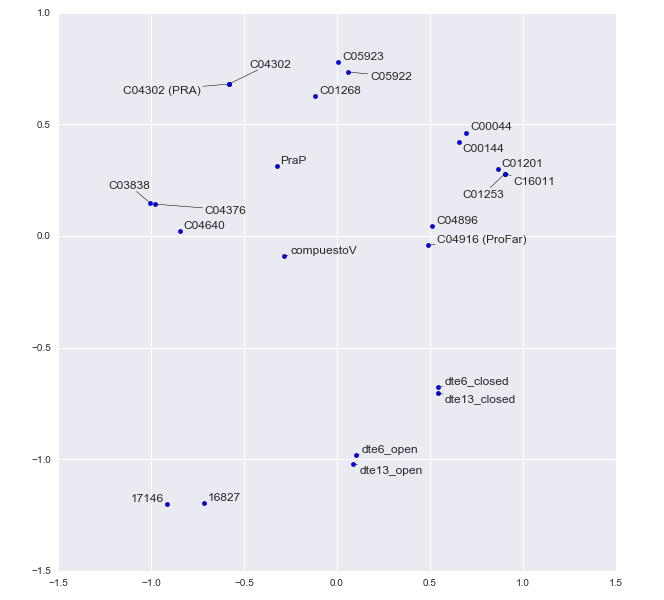
\includegraphics[angle = 0,scale = 0.4]{chapter4/SubstratesClustering.png}
  \caption[Clustering de sustratos de acuerdo a sus distancias de Tanimoto]{\footnotesize{Clustering de sustratos de acuerdo a sus distancias de Tanimoto}}
  \label{fig:tanimoto}
  \end{figure}
  
  \clearpage  
  
  \begin{figure}[h!tbp]
  \centering
  \includegraphics[angle = 0,scale = .8]{chapter4/SustratosQuimicos.pdf}
  \caption[Substatos químicamente similares a los sustratos de PriA (parte 1)]{\footnotesize{Substatos químicamente similares a los sustratos de PriA (parte 1)}}
  \label{fig:Eschema1}
  \end{figure}
  
  \begin{figure}[h!tbp]
  \centering
  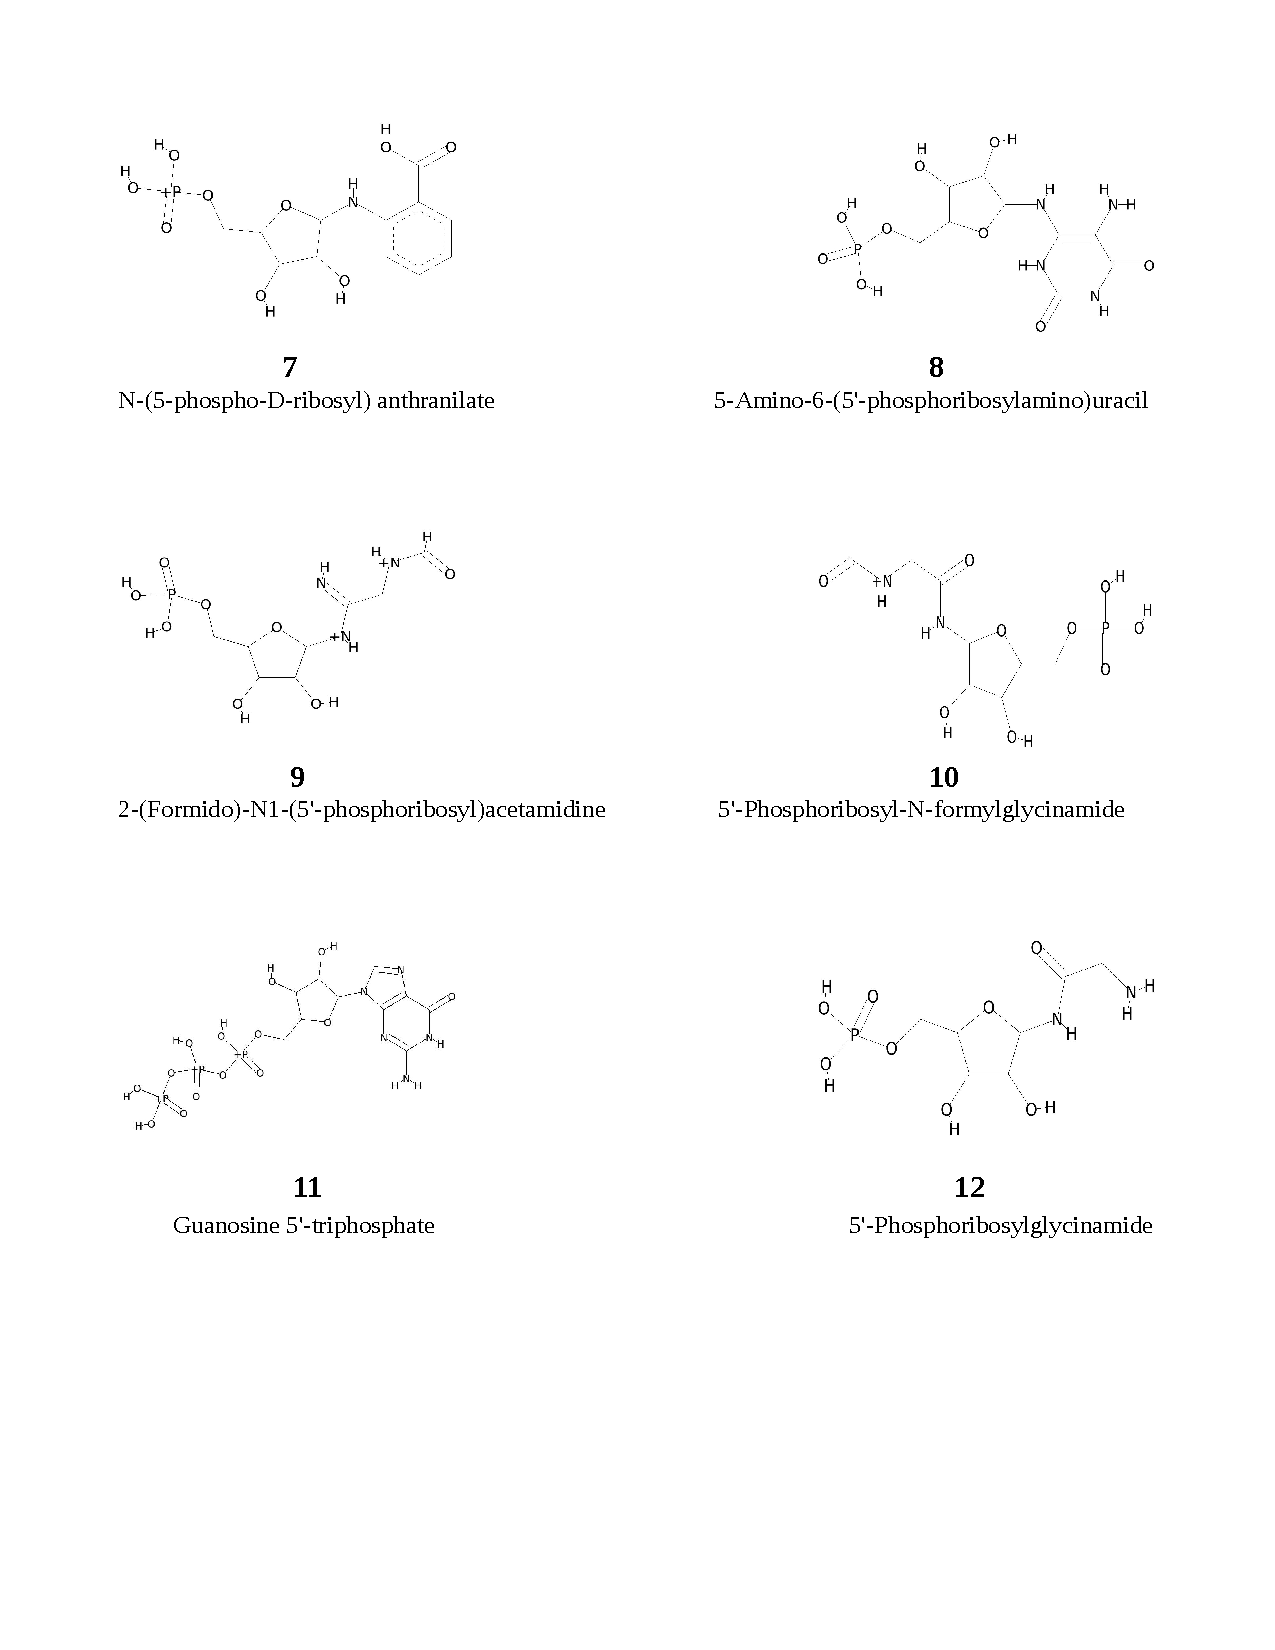
\includegraphics[angle = 0,scale = .8]{chapter4/esquema_quimico-2-2.pdf}
  \caption[Substatos químicamente similares a los sustratos de PriA (parte 2)]{\footnotesize{Substatos químicamente similares a los sustratos de PriA (parte 2)}}
  \label{fig:Eschema2}
  \end{figure}
  
  \begin{figure}[h!tbp]
  \centering
  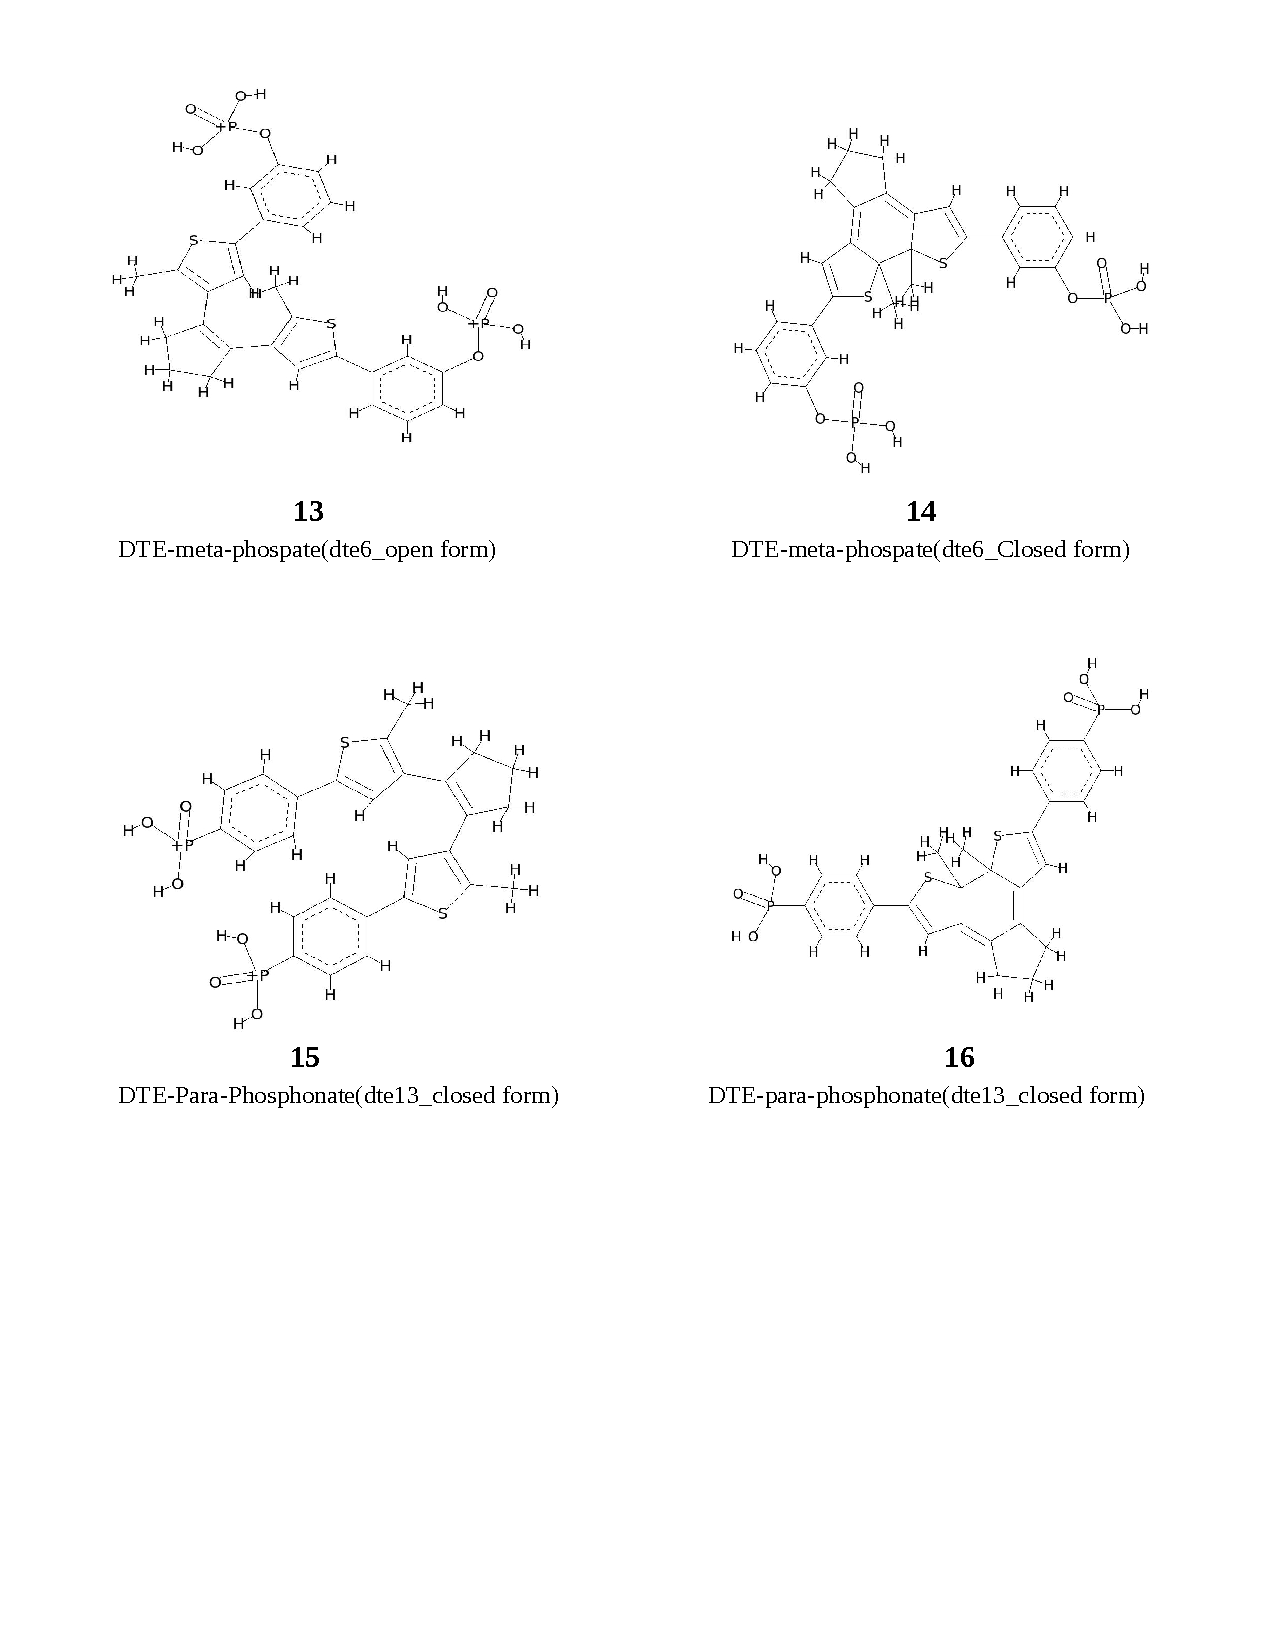
\includegraphics[angle = 0,scale = .8]{chapter4/esquema_quimico-3-3.pdf}
  \caption[Substatos químicamente similares a los sustratos de PriA (parte 3)]{\footnotesize{Substatos químicamente similares a los sustratos de PriA (parte 3)}}
  \label{fig:Eschema3}
  \end{figure}
  
  \begin{figure}[h!tbp]
  \centering
  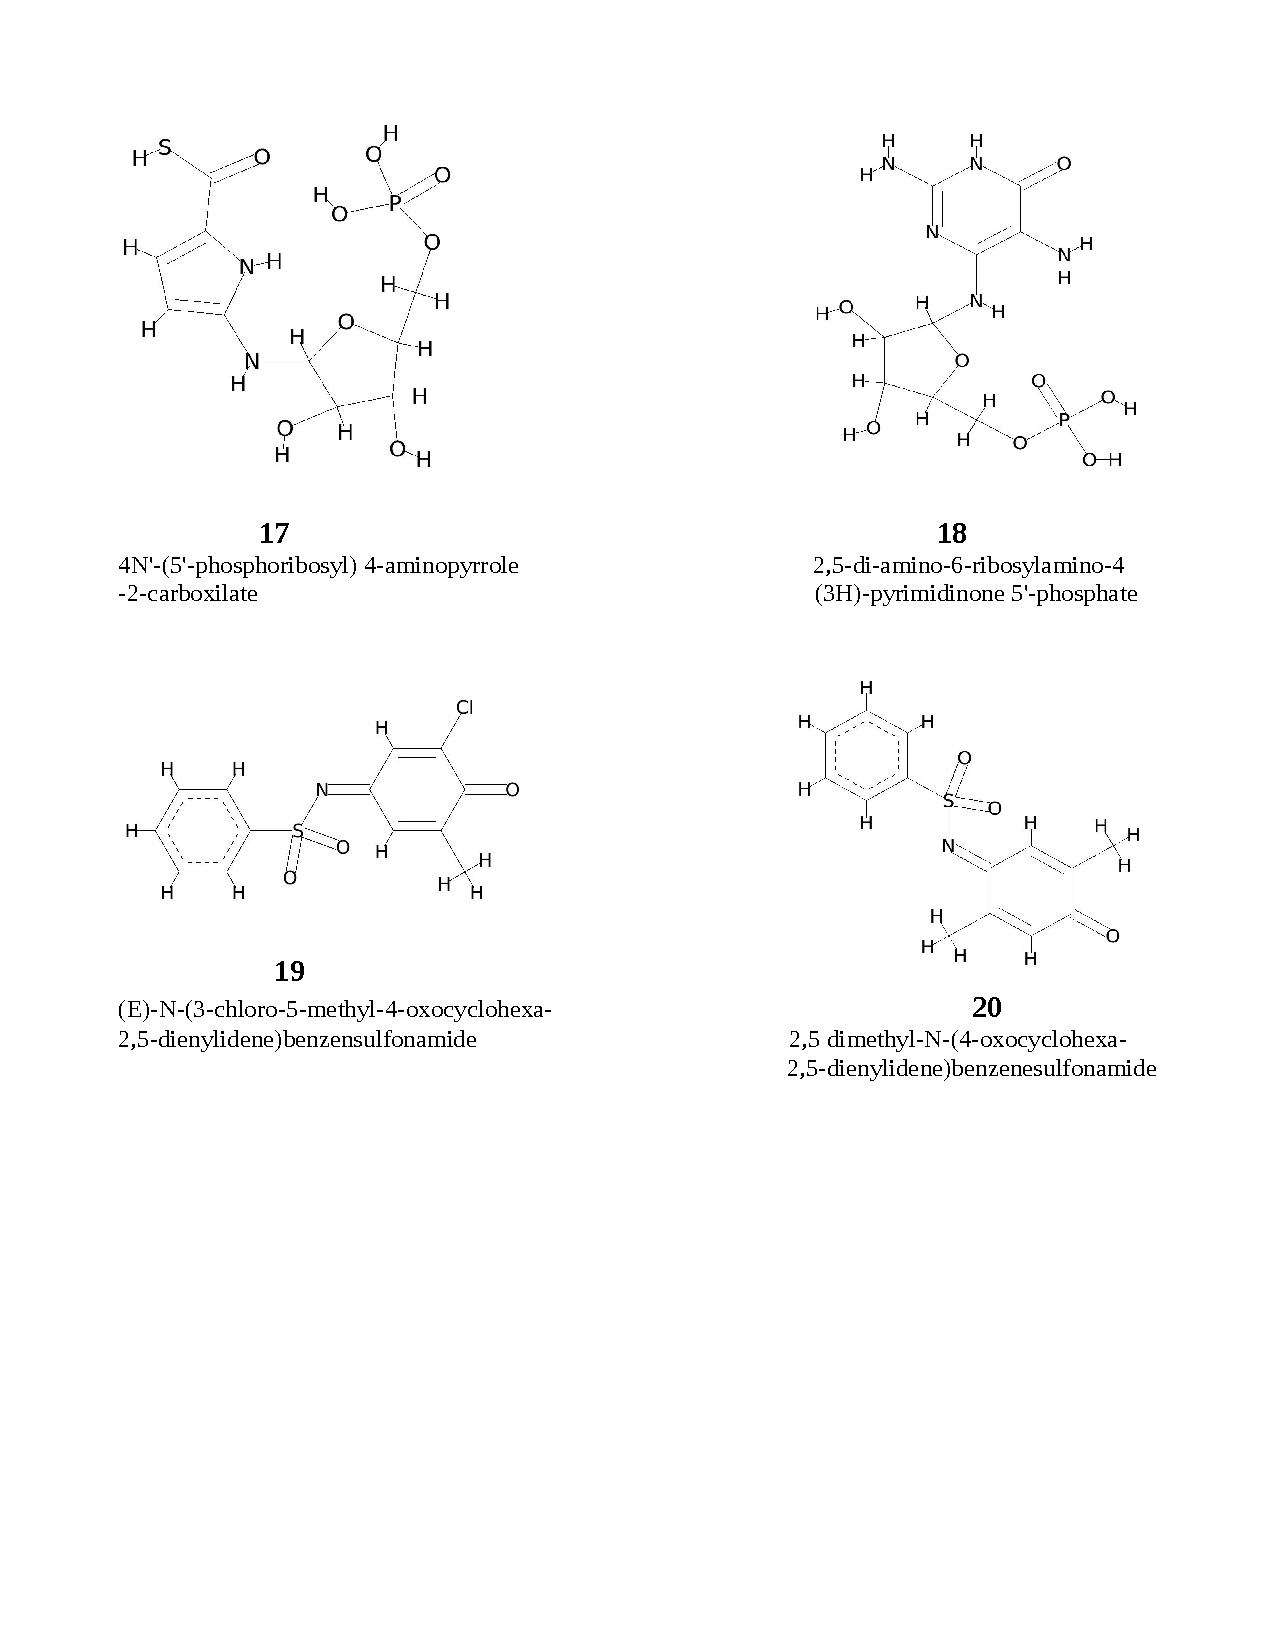
\includegraphics[angle = 0,scale = .8]{chapter4/esquema_quimico-4-4.pdf}
  \caption[Substatos químicamente similares a los sustratos de PriA (parte 4)]{\footnotesize{Substatos químicamente similares a los sustratos de PriA (parte 4)}}
  \label{fig:Eschema4}
  \end{figure}
  
  \clearpage  
  
  \subsection{Selección de secuencias de PriA o familias relacionadas para
  docking con sustratos similares a lo
  nativos}\label{seleccion-de-secuencias-de-pria-o-familias-relacionadas-para-docking-con-sustratos-similares-a-lo-nativos}
  
  Seleccioné 39 secuencias de la familia PriA para en colaboración con el
  grupo del Dr Carillo-Trip realizar el análisis bioinformático de
  acoplameinto del sustrato de la enzima de acoplamiento, entre ellas
  varios \emph{Streptomyces} dado que en ese género existen al menos dos
  familias, PriA y PriB. Estas secuencias seleccionadas de PriA / PriB
  están uniformemente distribuidas en un árbol de especies de
  \emph{Streptomyces} basado en la proteína RpoB. Estos Streptomyces
  tienen variedad en cuanto a la presencia / ausencia de TrpF. En esta
  sección se incluyeron otros homólogos de PriA Actinobacterial
  caracterizados químicamente, finalmente se agregaron secuencias de HisA
  de \emph{Escherichia coli}, \emph{Arthrobacter Aurescens},
  \emph{Salmonella enterica} y \emph{Acidimicrobium ferrooxidans} y para
  TrpF \emph{Jonesia denitrificans} y \emph{Streptomyces sp } Mg1 como
  controles.
  
  Cuando existían estructuras cristalográficas se utilizó esa estructura,
  de lo contrario, se generaron estructuras homólogas utilizando como
  plantilla la estructura de la enzima más cercana que contara estructura
  de cristalográfica. Los organismos que cuentan con estructura
  cristalográfica de alguna familia relacionada a PriA están descritos en
  la \autoref{tab:EnzymePDB}. Entre ellos están ejemplos de la familia
  HisA de Enterobacteria como \emph{Salmonella enterica} (PDB:5A-) y
  \emph{Thermotoga maritima} (2W79, 1QO2). Los representantes de TrpF son
  las Actinobacterias \emph{Jonesia denitrificans} y \emph{Streptomyces sp
  Mg1}. Entre las Actinobacterias caracterizadas con estructura
  cristalográfica de PriA están \emph{Mycobacterium tuberculosis} (Mtub
  PDB:2Y88,2Y89,2Y85,3ZS4), \emph{Streptomyces coelicolor} (Scoe
  PDB:2VEP,2X30,1VZW), \emph{Streptomyces globisporus}, \emph{Actynomyces
  urogenitalis} (4X2R) y \emph{Corynebacterium jeikeum}. De la familia
  subHisA se muestran \emph{Corynebacterium efficiens} y \emph{Actinomyces
  urogenitalis} (PDB:4X2R). Las estructuras cristalográficas disponibles
  de PriB provienen de \emph{Streptomyces ipomoeae}, \emph{Streptomyces
  sviceus} (PDB:4U28,4TX9). La estructura que representa a subTrpF es la
  de \emph{Arthrobacter aurescens} (PDB:4WD0) y finalmente, las
  estructuras de TrpF corresponden al las de los organismos \emph{Jonesia
  denitrificans} (PDB:4WUI) \emph{Chlamidya thrachomatis},
  \emph{Streptomyces sp. Mg1} y \emph{Actinomyces odontolyticus}.
  
  \clearpage  
  
  \begin{Shaded}
  \begin{Highlighting}[]
  \NormalTok{table <-}\StringTok{ }\KeywordTok{read.csv}\NormalTok{(}\StringTok{"chapter4/EstructurasPDB"}\NormalTok{, }\DataTypeTok{row.names =} \DecValTok{1}\NormalTok{,}\DataTypeTok{sep=}\StringTok{"}\CharTok{\textbackslash{}t}\StringTok{"}\NormalTok{)}
  \KeywordTok{kable}\NormalTok{(table,  }\DataTypeTok{caption =} \StringTok{"Estructuras cristalográficas disponibles de PriA y familias relacionadas }\CharTok{\textbackslash{}\textbackslash{}}\StringTok{label\{tab:EnzymePDB\}"}\NormalTok{,}\DataTypeTok{caption.short =} \StringTok{"Estructuras cristalográficas disponibles de PriA y familias relacionadas"}\NormalTok{)%>%}\StringTok{  }\KeywordTok{kable_styling}\NormalTok{(}\DataTypeTok{latex_options=}\StringTok{"scale_down"}\NormalTok{)}
  \end{Highlighting}
  \end{Shaded}
  
  \begin{table}[t]
  
  \caption[Estructuras cristalográficas disponibles de PriA y familias relacionadas]{\label{tab:Enzymes_PDB_out}Estructuras cristalográficas disponibles de PriA y familias relacionadas \label{tab:EnzymePDB}}
  \centering
  \resizebox{\linewidth}{!}{
  \begin{tabular}{l|l|l|l|r|r}
  \hline
    & Organismo & Family & Observations & Resolution & Year\\
  \hline
  5AHE & Salmonella enterica & HisA &  & 1.70 & 2015\\
  \hline
  5AB3 & Salmonella enterica & HisA & D7N, D10G, dup13-15, Q24L, G102A & 1.80 & 2016\\
  \hline
  5ABT & Salmonella enterica & HisA & D7N, G102A, V106M, D176A & 1.65 & 2016\\
  \hline
  5AC7 & Salmonella enterica & HisA & D7N, D10G, dup13-15 & 1.90 & 2016\\
  \hline
  5AC8 & Salmonella enterica & HisA & D10G, dup13-15, G102A & 1.70 & 2016\\
  \hline
  5AC6 & Salmonella enterica & HisA & D7N, D10G, dup13-15, Q24L, G102A & 1.99 & 2016\\
  \hline
  5A5W & Salmonella enterica & HisA & HisA D7N D176A with ProFAR & NA & 2015\\
  \hline
  5AHF & Salmonella enterica & HisA & HisA D7N with ProFAR & NA & NA\\
  \hline
  4GJ1 & Campylobacter jejuni & HisA &  & 2.15 & 2012\\
  \hline
  2W79 & Thermotoga maritima & HisA &  & 1.85 & 2008\\
  \hline
  1QO2 & Thermotoga maritima & HisA &  & 1.85 & 2000\\
  \hline
  4X9S & Streptomyces sp. MG1 & PriB &  & 1.60 & 2014\\
  \hline
  4TX9 & Streptomyces sviceus & PriB & ProFAR & 1.60 & 2014\\
  \hline
  4U28 & Streptomyces sviceus & PriB &  & 1.33 & 2014\\
  \hline
  4W9T & Streptomyces sp. Mg1 & PriB &  & 1.57 & 2014\\
  \hline
  4WD0 & Arthrobacter aurescens & subTrpF &  & 1.50 & 2014\\
  \hline
  5DN1 & Streptomyces coelicolor & PriA &  & 1.95 & 2015\\
  \hline
  1VZW & Streptomyces coelicolor & PriA &  & 1.80 & 2004\\
  \hline
  2VEP & Streptomyces coelicolor & PriA &  & 1.80 & 2007\\
  \hline
  2X30 & Streptomyces coelicolor & PriA & R139N & 1.95 & 2010\\
  \hline
  2Y85 & Mycobacterium tuberculosis & PriA & RCDRP & 2.40 & 2011\\
  \hline
  2Y88 & Mycobacterium tuberculosis & PriA & D11N PRFAR & 1.33 & 2011\\
  \hline
  2Y89 & Mycobacterium tuberculosis & PriA & D11N & 2.50 & 2011\\
  \hline
  3ZS4 & Mycobacterium tuberculosis & PriA & PRFAR & 1.90 & 2012\\
  \hline
  4X2R & Actinomyces urogenitalis & SubHisA &  & 1.05 & 2014\\
  \hline
  4AXK & Corynebacterium efficiens & SubHisA &  & 2.25 & 2013\\
  \hline
  5LHE & Thermococcus kodakaraensis & TrpF &  & 1.85 & 2016\\
  \hline
  5LHF & Thermococcus kodakaraensis & TrpF &  & 1.75 & 2016\\
  \hline
  1V5X & Thermus thermophilus & TrpF &  & 2.00 & 2003\\
  \hline
  1DL3 & Thermotoga maritima & TrpF &  & 2.70 & 1999\\
  \hline
  1LBM & Thermotoga maritima & TrpF & RCDRP & 2.80 & 2002\\
  \hline
  1NSJ & Thermotoga maritima & TrpF &  & 2.00 & 1996\\
  \hline
  4WUI & Jonesia denitrificans & TrpF &  & 1.09 & 2014\\
  \hline
  4AAJ & Pyrococcus furiosus & TrpF &  & 1.75 & 2012\\
  \hline
  \end{tabular}}
  \end{table}
  
  \subsection{El análisis de PriA a nivel estructural sugiere que GTP es
  el sustrato más
  afín}\label{el-analisis-de-pria-a-nivel-estructural-sugiere-que-gtp-es-el-sustrato-mas-afin}
  
  Con las enzimas seleccionadas de PriA se realizaron simulaciones de
  docking. Se incluyeron también como controles enzimas TrpF provenientes
  de \emph{Streptomyces Mg1, Jonesia denitrificans}. Los procedimientos
  pueden ser consultados en
  \href{https://github.com/tripplab/Docking/wiki}{Docking Protocols}. Como
  resultado podemos ver \autoref{fig:HeatplodPriAdocking} que el GTP es el
  que tiene mayor afinidad.
  
  \begin{figure}[h!tbp]
  \centering
  \includegraphics[angle = 0,scale = .7]{chapter4/Figura1_4.pdf}
  \caption[Heatplot del docking de enzimas relacionadas a PriA vs posibles substratos]{\footnotesize{Heatplot del docking de enzimas relacionadas a PriA vs posibles substratos}}
  \label{fig:HeatplodPriAdocking}
  \end{figure}
  
  \subsection{GTP es el sustrato por el que PriA muestra mayor
  afinidad}\label{gtp-es-el-sustrato-por-el-que-pria-muestra-mayor-afinidad}
  
  \begin{Shaded}
  \begin{Highlighting}[]
  \NormalTok{## boxplot de los sustratos}
  \KeywordTok{ggplot}\NormalTok{(docking.m, }\KeywordTok{aes}\NormalTok{(}\DataTypeTok{x=}\NormalTok{variable, }\DataTypeTok{y=}\NormalTok{value)) +}\StringTok{ }\KeywordTok{labs}\NormalTok{(}\DataTypeTok{x =} \StringTok{"Substrates"}\NormalTok{, }\DataTypeTok{y =} \StringTok{"Affinity"}\NormalTok{,}\DataTypeTok{text =} \KeywordTok{element_text}\NormalTok{(}\DataTypeTok{size=}\DecValTok{12}\NormalTok{)) +}\StringTok{ }\KeywordTok{geom_boxplot}\NormalTok{()+}\KeywordTok{theme_bw}\NormalTok{()+}\KeywordTok{theme}\NormalTok{(}\DataTypeTok{plot.title =} \KeywordTok{element_text}\NormalTok{(}\DataTypeTok{size =} \DecValTok{14}\NormalTok{, }\DataTypeTok{face =} \StringTok{"bold"}\NormalTok{), }\DataTypeTok{text =} \KeywordTok{element_text}\NormalTok{(}\DataTypeTok{size =} \DecValTok{12}\NormalTok{), }\DataTypeTok{axis.title =} \KeywordTok{element_text}\NormalTok{(}\DataTypeTok{face=}\StringTok{"bold"}\NormalTok{), }\DataTypeTok{axis.text.x=}\KeywordTok{element_text}\NormalTok{(}\DataTypeTok{angle =} \DecValTok{90}\NormalTok{,}\DataTypeTok{size =} \DecValTok{6}\NormalTok{), }\DataTypeTok{legend.position =} \StringTok{"bottom"}\NormalTok{)}
  \end{Highlighting}
  \end{Shaded}
  
  \begin{verbatim}
  Warning: Removed 100 rows containing non-finite values (stat_boxplot).
  \end{verbatim}
  
  \begin{center}\includegraphics{tesis_files/figure-latex/substrateBox-1} \end{center}
  
  \clearpage  
  
  \subsection{Dinámica molecular vs datos
  experimentales}\label{dinamica-molecular-vs-datos-experimentales}
  
  En las tablas \autoref{tab:PriAPRA} , \autoref{tab:PriAProFAR} se
  muestra a detalle la comparación entre las dinámicas moleculares de PriA
  respecto a PRA y ProFAR. Estos datos sugirieron que GTp es el sustrato
  con mayor afinidad y por ello en la última sección se avanzó en la
  realización de cinéticas enzimáticas con GTP.
  
  Table: Actividad de PriA en S3 PRA \label{tab:PriAPRA}
  
  \[ 
  \resizebox{\columnwidth}{!}{%
  \begin{tabular}{ l c r l l l l l}
  \hline \\ [-1.5ex]
  organism  &Family & $K_M    $     & $k_{cat}$        & $\frac{k_{cat}}{K_M}$ &Pre MD & Pos MD & Reference  \\ [1ex]
  \hline \\ [-1.5ex]
  Afer        &HisA   & $1.1\pm0.2$   &$  0.05\pm0.001    $& 0.045                  &-10.1    &-12.3       &Noda-García L et al 2015\\ [1ex]
  Ecoli       &HisA   &$  1.6         $&$         4.9       $&3.1                   &-9.9   &-16       &Henn-Sax et al. (2002)\\ [1ex]
  Sent        &HisA   &$  17.0 \pm0.1 $&$ 7.8 \pm 2.4   $&$4.5 × 10^5          $&-10.3  &-20.1     &Söderholm A et al (2015)\\ [1ex]
  Aaur        &PriB   &$  2.1 \pm 0.5 $& $    1.8 \pm 0.2     $&0.9                   &-7.4   &              &verduzco-castro 2016\\ [1ex]
  Sipo        &PriB   &$  3.8\pm0.2     $&$0.82\pm0.02        $&0.21                  &-8.2     &-14.7       &verduzco-castro 2016\\ [1ex]
  SspC        &PriB   &$  11.4\pm3.4  $&$2.53\pm0.74      $&0.22                  &   -8.5    &-12.7     &verduzco-castro 2016\\ [1ex]
  SMg1        &PriB   &$  13.2\pm3.4  $&$0.92\pm0.19      $&0.069                 &-8     &-15.2     &verduzco-castro 2016\\ [1ex]
  Ssvi        &PriB   &$  3.9\pm0.89  $&$0.69\pm0.04      $&0.18                  &-8.2     &-16.7     &verduzco-castro 2016\\ [1ex]
  Scoe        &PriA   &$  3.6\pm0.7     $&$ 1.3\pm0.2     $  &0.4                   &-8.4   &-15       &Noda-García et al (2010)\\ [1ex]
  Sglob       &PriA   & $4.2\pm0.8     $ & $0.74\pm0.03    $   &0.18                  &-9.2     &-16.7       &verduzco-castro\\ [1ex]
  Mtub 2Y85   &priA   &$  19  0.23      $&$0.012  -9.7          $&                      &       &          &Due et al 2011\\ [1ex]
  Mtub 3ZS4   &priA   &$  ?                 $&$-9.9               $&                      &       &          &Due et al 2011 (To be published)\\ [1ex]
  Auro        &priA   &$  4.0 \pm 0.9 $&$0.2 \pm 0.03   $&0.04                    &-9.2       &          &Vazquez-Juarez (2016)\\ [1ex]
  Cjei        &PriA   &$  2.3 \pm 0.2 $&$0.9 \pm 0.08   $&0.39                    &-8.5       &          &Noda-García et al (2013)\\ [1ex]
  Cdip        &subHisA&$  4.4 \pm 0.5 $&$2.6 \pm 0.3      $&0.59                  &-9.2       &          &Noda-García et al (2013)\\ [1ex]
  SMg1 TrpF   &TrpF3  &   -                &-                &-                       &-6.9     &-9.6      &verduzco-castro 2016\\ [1ex]
  Jden        &TrpF3  &   -                &-                &-          -7.2         &-9.4     &$16.8\pm3.3$&    Verduzco-Castro E et al  2016\\ [1ex]
  Acar      &SubHisA& 0.02                     &                 &                        &       &          &            \\ [1ex]
  Aodo        &SubTrpF&       -              &-                  &-                     &       &          &\\ [1ex]
  \hline
  \end{tabular}}
  \label{tab:PriAPRA}  
  %}
  \]
  
  \clearpage   La siguiente tabla es análoga a la anterior pero con el
  sustrato ProFAR
  
  Table: Actividad de PriA en S7 ProFAR \label{tab:PriAProFAR}
  
  \[ 
  \resizebox{\columnwidth}{!}{%
  \centering 
  \begin{tabular}{ l c r l l l l l}
  \hline \\ [-1.5ex]
  organism  &Family  &  $K_M$ & $k_{cat}$& $\frac{k{cat}}{K_M}$ &Pre MD &Pos MD &Reference  \\ [1ex]
  \hline \\ [-1.5ex]
  Afer      &HisA    &-            &-                &-          &-9.2    &-9        &Noda-García L et al. (2015)   \\ [1ex]
  Ecoli     &HisA    &-            &-                &-          &-9      &-11.1     &Henn-Sax et al. (2002)\\ [1ex]
  Sent      &HisA    &-            & -               &-          &-9.6    &-10.2     &Söderholm A et al (2015)\\ [1ex]
  Aaur      &PriB    &$26.3\pm6.3$ & $0.37\pm 0.09$  & 0.014     &-7.1    &-         &verduzco-castro 2016\\ [1ex]
  Sipo      &PriB    &$60.8\pm1.1$ &$8.25\pm0.4 $    &0.14       &-8      &-8.5      &verduzco-castro 2016 \\ [1ex]
  SspC      &PriB    &$149.9\pm29$ &$1.4\pm0.12 $    &0.009      &-8.5    &-10.8     &verduzco-castro 2016\\ [1ex]
  SMg1      &PriB    &$129.6\pm34$ &$0.29\pm0.04$    &0.0022     &-7.5    &-11       &verduzco-castro 2016\\ [1ex]
  Ssvi      &PriB    &$24.5\pm4.0$ &$1.6\pm0.29 $    &0.067      &-8      &-9.7      &verduzco-castro 2016 \\ [1ex]
  Scoe      &PriA    &$5.0\pm0.08$ &$3.4\pm0.09  $   &0.7        &-8      &-9.4      &Noda-García et al (2010)   \\ [1ex]
  Sglob     &PriA    &$11\pm1.0$  &$3.8\pm0.2  $     &0.34       &-8.7    &-9.4      &verduzco-castro 2016  \\ [1ex]
  Mtub2Y85  &priA    &21         &3.6         &0.17       &-8.6    &          &Due et al 2011                        \\ [1ex] 
  Mtub3ZS4  &priA    &           &            &           &-9.3    &          &Due et al 2011 (To be published)      \\ [1ex] 
  Auro      &priA    &$23 \pm 6.5 $  &$0.5\pm0.05 $&0.02       &-9.3    &          &Vazquez-Juarez (2016)                 \\ [1ex] 
  Cjei      &PriA    &$5.1 \pm1.0$  &$1.6 \pm 0.16 $&0.31       &-9      &          &Noda-García et al (2013)              \\ [1ex]
  Cdip      &subHisA &-          &-           &-          &-8.8    &          &Noda-García et al (2013)              \\ [1ex]
  SMg1 TrpF &TrpF3   &$8.4\pm1.7$    &$10.5\pm2.4$    &1.25       &-7.6    &-9        &verduzco-castro     \\ [1ex] 
  Jden      &TrpF3   &$16.8\pm3.3$   &$27\pm1.6$      &1.6        &-7.6    &-7.7      &verduzco-castro     \\ [1ex] 
  Acar      &SubHisA &Na         &Na          &0.02       &Na      &Na        &Na                                    \\ [1ex] 
  Aodo      &SubTrpF &-          &-           &-          &-       &Na        &Na                                    \\ [1ex]
  \hline
  \end{tabular}}
  \label{tab:PriAProFAR}    
  %}  
  \]
  
  \begin{table}[t]
  
  \caption[Enzymes docking ]{\label{tab:docking_table_out}Enzymes docking \label{tab:docking}}
  \centering
  \resizebox{\linewidth}{!}{
  \begin{tabular}{l|r|r|r|r|r|r|r|r|r|r|r|r|r|r|r|r|r|r|r|r}
  \hline
  Enzima & S13 & S15 & S14 & S16 & S10 & S12 & S9 & S18 & S5 & S4 & S8 & S17 & S7 & S6 & S11 & S1 & S2 & S3 & S19 & S20\\
  \hline
  Srub\_2VEP & -7.4 & -7.3 & -7.5 & -7.1 & -6.5 & -6.2 & -6.5 & -7.7 & -9.4 & -9.3 & -7.9 & -7.2 & -8.3 & -8.6 & -8.9 & -9.0 & -7.1 & -8.9 & -7.8 & -7.7\\
  \hline
  Saver\_2VEP & -7.4 & -7.2 & -7.0 & -6.5 & -7.3 & -6.4 & -7.0 & -7.5 & -9.6 & -8.5 & -7.9 & -7.6 & -8.4 & -8.7 & -9.8 & -8.3 & -7.9 & -8.6 & -7.7 & -7.6\\
  \hline
  Scoe\_2VEP & -7.5 & -7.5 & -7.9 & -7.0 & -7.0 & -6.2 & -6.5 & -7.8 & -8.8 & -9.2 & -7.8 & -7.9 & -8.0 & -8.9 & -10.3 & -9.2 & -9.3 & -8.4 & -8.1 & -8.2\\
  \hline
  Scoe\_2X30 & -8.1 & -7.4 & -7.6 & -6.9 & -6.7 & -6.8 & -7.1 & -7.9 & -9.1 & -9.0 & -8.3 & -8.6 & -8.5 & -9.0 & -10.6 & -10.0 & -10.3 & -10.2 & -8.1 & -7.9\\
  \hline
  Scoe\_1VZW & NA & NA & NA & NA & NA & NA & NA & NA & NA & NA & NA & NA & NA & NA & NA & NA & NA & NA & NA & NA\\
  \hline
  Sfla\_2VEP & -7.1 & -7.6 & -7.2 & -7.3 & -7.2 & -6.8 & -6.9 & -8.1 & -8.2 & -7.2 & -8.2 & -7.2 & -8.4 & -8.3 & -8.5 & -7.9 & -7.8 & -6.0 & -7.5 & -7.3\\
  \hline
  Sgha\_2VEP & -9.2 & -8.7 & -6.7 & -6.7 & -7.4 & -7.7 & -7.2 & -7.5 & -9.8 & -8.9 & -8.2 & -7.8 & -8.8 & -8.7 & -10.1 & -9.1 & -9.0 & -9.5 & -8.0 & -7.5\\
  \hline
  Siak\_2VEP & -6.6 & -7.3 & -7.0 & -7.1 & -7.1 & -7.1 & -6.8 & -8.0 & -9.2 & -8.7 & -7.8 & -7.6 & -8.3 & -8.4 & -9.1 & -5.8 & -5.3 & -8.5 & -7.3 & -7.4\\
  \hline
  Sbic\_2VEP & -7.2 & -6.7 & -6.8 & -6.5 & -6.2 & -6.6 & -5.9 & -7.8 & -8.5 & -7.8 & -7.8 & -7.2 & -8.2 & -8.0 & -9.6 & -8.2 & -8.0 & -9.4 & -7.7 & -7.5\\
  \hline
  Sbot\_2VEP & -9.6 & -10.9 & -8.9 & -7.1 & -6.0 & -6.2 & -6.7 & -8.1 & -9.1 & -8.8 & -8.3 & -7.9 & -8.9 & -9.3 & -9.4 & -9.8 & -10.0 & -8.9 & -8.2 & -8.0\\
  \hline
  Sipo\_2VEP & -6.6 & -6.6 & -7.3 & -6.9 & -6.5 & -6.3 & -6.5 & -8.1 & -8.6 & -9.1 & -8.0 & -7.9 & -8.0 & -8.4 & -8.5 & -7.2 & -8.4 & -8.2 & -7.9 & -7.6\\
  \hline
  Ssvi & NA & NA & NA & NA & NA & NA & NA & NA & NA & NA & NA & NA & NA & NA & NA & NA & NA & NA & NA & NA\\
  \hline
  Ssvi\_4U28 & NA & NA & NA & NA & NA & NA & NA & NA & NA & NA & NA & NA & NA & NA & NA & NA & NA & NA & NA & NA\\
  \hline
  Ssvi\_4TX9 & -5.9 & -8.2 & -7.1 & -6.6 & -6.8 & -7.0 & -7.6 & -7.9 & -8.4 & -8.3 & -8.2 & -8.1 & -8.4 & -8.7 & -7.7 & -8.2 & -8.2 & -6.7 & -8.0 & -7.5\\
  \hline
  Salb\_2VEP & -6.3 & -7.1 & -7.4 & -6.8 & -7.7 & -6.9 & -6.6 & -8.0 & -9.6 & -8.9 & -8.6 & -7.9 & -8.6 & -8.4 & -9.1 & -7.4 & -7.2 & -8.8 & -8.1 & -7.8\\
  \hline
  Sbik\_2VEP & -7.4 & -6.7 & -7.4 & -7.3 & -7.7 & -6.5 & -6.8 & -8.5 & -9.9 & -9.8 & -8.3 & -7.8 & -8.2 & -8.4 & -10.5 & -7.1 & -6.3 & -8.3 & -8.1 & -7.9\\
  \hline
  Stsu\_2VEP & -6.9 & -7.5 & -7.9 & -7.8 & -7.5 & -7.3 & -7.7 & -8.1 & -10.0 & -9.7 & -8.7 & -7.8 & -8.8 & -8.8 & -10.6 & -7.8 & -8.7 & -9.2 & -7.9 & -7.8\\
  \hline
  Sven\_2VEP & -8.3 & -7.6 & -7.5 & -6.8 & -6.4 & -7.0 & -6.2 & -8.2 & -9.6 & -9.0 & -7.9 & -7.4 & -8.3 & -8.6 & -10.0 & -8.2 & -8.2 & -8.1 & -7.6 & -7.4\\
  \hline
  Scal\_2VEP & -7.3 & -8.8 & -7.5 & -6.7 & -7.0 & -6.5 & -6.5 & -8.7 & -10.0 & -9.7 & -8.8 & -7.7 & -8.2 & -8.6 & -10.5 & -8.1 & -9.2 & -8.9 & -7.6 & -7.6\\
  \hline
  Sbaa\_2VEP & -8.9 & -6.6 & -6.7 & -6.8 & -7.2 & -7.2 & -6.2 & -7.7 & -9.6 & -9.5 & -8.4 & -7.4 & -8.5 & -8.2 & -9.7 & -8.5 & -8.4 & -9.3 & -7.4 & -7.7\\
  \hline
  Sglo\_2VEP & -6.1 & -6.8 & -6.9 & -6.5 & -6.7 & -6.3 & -6.7 & -7.5 & -9.6 & -9.6 & -8.6 & -7.8 & -8.7 & -8.7 & -9.9 & -6.2 & -5.1 & -9.2 & -7.8 & -7.7\\
  \hline
  Sful\_2VEP & -9.0 & -6.9 & -7.1 & -6.8 & -6.3 & -7.2 & -6.6 & -8.1 & -9.8 & -9.3 & -7.7 & -8.0 & -8.7 & -8.8 & -10.5 & -7.6 & -9.1 & -10.5 & -7.1 & -7.4\\
  \hline
  Sgri\_2VEP & -6.6 & -8.2 & -7.1 & -6.4 & -7.1 & -7.4 & -7.1 & -7.4 & -9.4 & -8.5 & -8.6 & -7.5 & -8.8 & -8.4 & -9.6 & -8.8 & -8.8 & -8.7 & -7.7 & -7.5\\
  \hline
  S34\_2VEP & -7.8 & -7.2 & -7.6 & -7.3 & -6.2 & -6.5 & -6.9 & -8.0 & -8.8 & -8.6 & -7.7 & -7.1 & -7.7 & -7.9 & -7.2 & -7.1 & -6.7 & -7.1 & -7.7 & -7.7\\
  \hline
  Srim\_2VEP & -7.4 & -6.8 & -7.1 & -7.2 & -7.2 & -7.4 & -7.8 & -8.6 & -9.7 & -9.3 & -8.8 & -7.7 & -8.9 & -8.7 & -10.2 & -6.8 & -8.2 & -9.0 & -7.5 & -7.8\\
  \hline
  Satr\_2VEP & -7.6 & -7.1 & -7.5 & -7.4 & -6.2 & -6.5 & -6.9 & -8.0 & -8.9 & -8.7 & -7.7 & -7.4 & -7.7 & -7.8 & -6.5 & -7.0 & -6.3 & -7.7 & -7.7 & -7.7\\
  \hline
  S1813\_2VEP & -7.5 & -6.7 & -6.8 & -6.6 & -6.8 & -7.0 & -6.7 & -7.9 & -9.9 & -9.7 & -8.3 & -7.7 & -8.5 & -8.6 & -10.0 & -7.6 & -7.5 & -8.6 & -7.3 & -7.5\\
  \hline
  Svar\_2VEP & -6.3 & -6.8 & -7.0 & -6.3 & -6.9 & -6.9 & -6.6 & -7.8 & -9.3 & -7.4 & -8.5 & -7.3 & -8.0 & -8.7 & -8.5 & -7.4 & -6.3 & -6.0 & -7.9 & -7.5\\
  \hline
  Sfra\_2VEP & -7.3 & -7.0 & -6.8 & -6.6 & -6.5 & -7.3 & -6.6 & -8.6 & -9.1 & -8.7 & -8.9 & -7.7 & -8.9 & -9.0 & -8.7 & -6.0 & -6.3 & -7.9 & -8.2 & -7.8\\
  \hline
  Smeg\_2VEP & -8.0 & -7.3 & -6.9 & -6.6 & -7.2 & -6.7 & -6.1 & -7.6 & -9.2 & -9.1 & -7.8 & -7.4 & -8.2 & -8.5 & -9.6 & -9.2 & -9.2 & -8.6 & -7.7 & -7.5\\
  \hline
  Ssul\_2VEP & -7.5 & -7.0 & -6.9 & -6.6 & -6.6 & -6.7 & -6.9 & -7.7 & -8.4 & -8.2 & -8.2 & -7.5 & -8.1 & -7.7 & -8.2 & -6.7 & -7.1 & -7.7 & -7.6 & -7.4\\
  \hline
  Slav\_4X9S & -8.0 & -7.1 & -6.7 & -6.9 & -6.6 & -6.8 & -6.7 & -8.2 & -9.5 & -9.1 & -8.6 & -8.0 & -8.4 & -8.7 & -9.1 & -9.5 & -9.3 & -8.1 & -8.1 & -7.6\\
  \hline
  Sery\_4X9S & -7.8 & -7.2 & -7.6 & -7.2 & -7.4 & -6.9 & -7.4 & -8.5 & -9.4 & -9.4 & -8.6 & -7.6 & -8.4 & -8.6 & -9.1 & -10.0 & -10.1 & -9.0 & -7.8 & -8.2\\
  \hline
  SspC\_4X9S & -7.4 & -6.9 & -7.3 & -6.8 & -7.3 & -6.6 & -7.5 & -8.0 & -9.8 & -9.3 & -8.7 & -7.6 & -8.5 & -8.4 & -10.6 & -9.1 & -8.9 & -8.5 & -8.1 & -8.0\\
  \hline
  Sxan\_4X9S & -7.5 & -6.9 & -6.8 & -6.8 & -6.5 & -6.6 & -6.5 & -8.3 & -8.0 & -8.1 & -7.6 & -7.4 & -8.7 & -8.1 & -8.1 & -8.5 & -8.0 & -7.6 & -7.7 & -7.4\\
  \hline
  Skat\_4X9S & -6.4 & -7.0 & -7.1 & -6.7 & -7.7 & -6.3 & -6.2 & -8.1 & -8.5 & -9.2 & -8.3 & -7.6 & -9.0 & -8.5 & -9.7 & -9.5 & -9.9 & -9.2 & -7.4 & -7.5\\
  \hline
  SMg1\_4X9S & -6.5 & -6.9 & -7.2 & -7.1 & -6.5 & -6.9 & -6.4 & -7.3 & -7.8 & -7.7 & -8.3 & -7.5 & -7.9 & -8.4 & -9.5 & -7.6 & -5.2 & -7.5 & -7.6 & -7.7\\
  \hline
  SMg1\_W9T & NA & NA & NA & NA & NA & NA & NA & NA & NA & NA & NA & NA & NA & NA & NA & NA & NA & NA & NA & NA\\
  \hline
  Sniv\_2VEP & -6.2 & -6.8 & -7.4 & -6.5 & -7.8 & -6.8 & -6.7 & -9.5 & -9.6 & -9.4 & -8.7 & -8.2 & -8.6 & -9.1 & -9.9 & -5.4 & -5.5 & -9.2 & -8.0 & -7.5\\
  \hline
  Scla\_2VEP & -6.4 & -7.7 & -7.4 & -7.2 & -7.6 & -7.5 & -7.2 & -8.5 & -10.1 & -10.0 & -8.7 & -7.9 & -8.8 & -9.1 & -10.2 & -6.9 & -8.1 & -8.5 & -7.7 & -7.7\\
  \hline
  Save\_2VEP & -7.6 & -6.7 & -7.1 & -7.2 & -7.1 & -6.5 & -6.6 & -7.8 & -8.6 & -10.0 & -8.6 & -7.5 & -8.3 & -8.5 & -8.8 & -5.3 & -5.2 & -5.8 & -7.7 & -7.4\\
  \hline
  Spur\_2vEP & -6.8 & -7.3 & -6.9 & -6.7 & -8.0 & -7.9 & -7.7 & -8.5 & -9.5 & -9.8 & -8.1 & -7.8 & -8.7 & -9.7 & -10.0 & -5.3 & -6.2 & -8.2 & -7.6 & -7.4\\
  \hline
  Scar\_2Y89 & -6.9 & -6.8 & -7.5 & -7.1 & -7.8 & -7.3 & -7.2 & -8.3 & -9.2 & -8.3 & -8.9 & -8.4 & -8.9 & -9.3 & -9.4 & -5.3 & -5.2 & -7.1 & -8.5 & -8.6\\
  \hline
  Mtub\_2Y88 & -10.0 & -7.8 & -8.9 & -5.4 & -8.6 & -7.3 & -7.8 & -9.5 & -10.9 & -10.3 & -9.5 & -9.0 & -9.8 & -9.8 & -11.3 & -10.1 & -10.2 & -11.3 & -9.5 & -8.8\\
  \hline
  Mtub\_2Y89 & -8.7 & -8.6 & -9.6 & -9.4 & -6.4 & -5.9 & -5.6 & -7.1 & -7.0 & -7.5 & -7.3 & -6.8 & -7.4 & -8.4 & -7.5 & -8.1 & -8.6 & -7.5 & -7.7 & -7.3\\
  \hline
  Mtub\_2Y85 & -8.2 & -7.9 & -9.2 & -7.4 & -7.6 & -7.5 & -7.6 & -8.4 & -9.7 & -9.5 & -9.3 & -7.8 & -8.6 & -8.6 & -10.2 & -9.8 & -9.9 & -10.1 & -7.3 & -7.4\\
  \hline
  Mtub\_3ZS4 & -10.0 & -10.5 & -11.4 & -6.4 & -8.2 & -7.2 & -7.0 & -9.6 & -10.2 & -10.2 & -9.9 & -8.5 & -9.3 & -9.6 & -10.9 & -10.0 & -10.7 & -9.9 & -8.8 & -8.9\\
  \hline
  S34\_3ZS4 & -7.4 & -8.0 & -7.6 & -6.4 & -5.2 & -5.4 & -5.2 & -6.1 & -6.8 & -6.4 & -5.7 & -6.4 & -6.3 & -6.3 & -7.1 & -7.4 & -7.1 & -6.4 & -7.1 & -6.6\\
  \hline
  Cdip\_4AXK & -9.2 & -7.8 & -10.9 & -7.2 & -7.5 & -7.6 & -7.7 & -8.9 & -9.0 & -9.8 & -9.0 & -8.3 & -8.8 & -9.2 & -10.1 & -9.5 & -9.9 & -9.2 & -8.0 & -7.9\\
  \hline
  Cjei\_4AXK & -7.5 & -6.9 & -7.2 & -6.5 & -8.4 & -8.0 & -8.5 & -8.7 & -9.5 & -9.6 & -9.4 & -8.8 & -9.0 & -9.5 & -9.3 & -8.1 & -9.3 & -8.5 & -7.9 & -7.7\\
  \hline
  Aaur & NA & NA & NA & NA & NA & NA & NA & NA & NA & NA & NA & NA & NA & NA & NA & NA & NA & NA & NA & NA\\
  \hline
  Aaur\_4WD0 & -8.2 & -8.5 & -8.1 & -7.9 & -5.7 & -5.5 & -5.9 & -7.0 & -7.5 & -7.2 & -7.1 & -6.7 & -7.1 & -7.4 & -8.4 & -7.2 & -7.3 & -7.4 & -7.0 & -6.7\\
  \hline
  Acar\_4X2R & -10.6 & -9.3 & -9.3 & -7.2 & -7.2 & -6.8 & -7.3 & -7.5 & -9.5 & -9.8 & -8.0 & -7.8 & -9.3 & -8.9 & -10.3 & -9.6 & -9.4 & -9.4 & -8.1 & -8.0\\
  \hline
  Auro\_4X2R & -9.9 & -9.1 & -9.8 & -8.1 & -7.4 & -7.1 & -7.4 & -7.8 & -9.2 & -9.8 & -8.3 & -7.8 & -9.3 & -9.0 & -9.9 & -9.0 & -8.6 & -9.2 & -8.5 & -8.2\\
  \hline
  Afer\_4WD0 & -5.7 & -5.8 & -6.0 & -5.7 & -6.7 & -6.2 & -5.8 & -7.6 & -9.2 & -8.8 & -7.8 & -7.4 & -8.3 & -8.4 & -9.3 & -6.7 & -4.5 & -9.1 & -8.3 & -8.1\\
  \hline
  Sent\_5AHE & -9.1 & -5.4 & -6.4 & -5.2 & -8.0 & -7.3 & -7.4 & -8.8 & -10.7 & -10.2 & -8.7 & -8.7 & -9.6 & -9.9 & -10.9 & -7.8 & -9.1 & -10.3 & -9.0 & -8.4\\
  \hline
  Ecoli\_K12 & -9.7 & -9.7 & -9.2 & -6.1 & -7.2 & -6.6 & -6.8 & -8.6 & -9.5 & -9.1 & -8.6 & -8.2 & -9.0 & -8.6 & -10.2 & -9.9 & -10.2 & -9.9 & -8.2 & -7.9\\
  \hline
  Jden\_4WUI & -8.3 & -8.8 & -8.2 & -6.8 & -6.2 & -6.1 & -6.0 & -6.8 & -7.4 & -7.6 & -7.5 & -6.9 & -7.6 & -7.5 & -7.7 & -7.5 & -7.6 & -7.2 & -7.3 & -7.2\\
  \hline
  Ctra & -8.2 & -8.0 & -7.4 & -7.2 & -6.1 & -5.5 & -5.4 & -6.5 & -7.1 & -7.1 & -7.0 & -6.2 & -6.8 & -6.8 & -6.9 & -7.2 & -7.4 & -6.5 & -6.7 & -6.6\\
  \hline
  SMg1\_trpF & -7.2 & -8.8 & -8.2 & -7.3 & -6.2 & -5.7 & -5.7 & -6.9 & -6.6 & -6.7 & -7.3 & -6.7 & -7.6 & -6.9 & -7.5 & -7.1 & -7.1 & -6.9 & -6.7 & -6.5\\
  \hline
  Aodo\_4X2R & -8.5 & -8.6 & -8.8 & -7.3 & -7.1 & -7.1 & -7.1 & -7.5 & -9.7 & -9.4 & -7.8 & -7.6 & -9.6 & -8.8 & -10.1 & -8.4 & -8.9 & -9.4 & -8.0 & -8.1\\
  \hline
  \end{tabular}}
  \end{table}
  
  Con actividad de FolE i.e activa para el compuesto V Adams et al (2014)
  
  \clearpage  
  
  \section{PriA en cinéticas enzimáticas no
  tradicionales.}\label{pria-en-cineticas-enzimaticas-no-tradicionales.}
  
  Además de la exploración genómica de PriA se realizaron
  caracterizaciones experimentales. No se tuvo el tiempo ni la experiencia
  para tener réplicas de los resultados descritos a continuación, sin
  embargo pueden ser un buen comienzo para futuros estudiantes que deseen
  retomarlos. Todos los protocolos fueron cuidadosamente descritos y se
  encuentran en los anexos. Este capítulo se enfoca en el montaje de dos
  experimentos. \emph{i)} Cinéticas de PriA en GTP . \emph{ii)} Medición
  simultánea de la actividad de PriA sobre ProFAR y PRA.
  
  Lo primero que se realizó fue la sobre expresión heteróloga de PriA y su
  respectiva purificación para poder realizar \emph{in vitro} cinéticas
  enzimáticas. Las enzimas fueron clonadas en cepas de \emph{E. coli} V68
  se indujo sobre expresión y se purifico la proteína. Se corroboró el
  éxito de esta actividad mediante un gel de proteína en la que puede
  verse expresión en la barra correspondiente al tamaño de PriA
  \autoref{fig:gel}.
  
  \begin{figure}[h!tbp]
  \centering
  \includegraphics[angle = 0,scale = 0.6]{chapter4/Geles/PriAAbril30.png}
  \caption[gel]{\footnotesize{Gel de proteína donde se muestra la banda correspondiente a PriA después de ser sobre-expresada y purificada}}
  \label{fig:gel}
  \end{figure}
  
  Con la proteína purificada y almacenada a -80° en esferas de proteína
  selladas con nitrógeno líquido como se describe en el anexo de los
  procedimientos se procedió a realizar cinéticas enzimáticas.
  
  \subsection{PriA puede tener actividad en
  GTP}\label{pria-puede-tener-actividad-en-gtp}
  
  La actividad fue medida fluorometricamente en placas de 96 (Nuc 96-Well
  Optical Botto Plates) en un lector de placas TECAN infinite M1000 (con
  exitación a 286 nm y emisión a 386 nm). Ensayos preliminares de
  actividad se realizaron en una PriA activa respecto a los otros
  substratos y proveniente de \emph{Streptomyces coelicolor} y en la
  mutante inactiva D11A.
  
  \begin{figure}[h!tbp]
  \centering
  \includegraphics[angle = 0,scale = 0.8]{chapter4/MutantControl.png}
  \caption[Scoe and non functional Scoe PriA acting on dGTP]{\footnotesize{}}
  \label{fig:PriARutas1}
  \end{figure}
  
  \begin{figure}[h!tbp]
  \centering
  \includegraphics[angle = 0,scale = 0.6]{chapter4/GTPCinetica.pdf}
  \caption[Scoe and non functional Scoe PriA acting on dGTP]{\footnotesize{}}
  \label{fig:PriARutas2}
  \end{figure}
  
  \clearpage  
  
  Entre las enzimas donde se aprecia actividad está \emph{Thermomonospora
  curvata} que es una Actinobacteria termofílica de la familia
  \emph{Thermomonosporaceae} y que puede ser encontrada encompostas ya que
  participa en la degradación de celulosa
  {[}\protect\hyperlink{ref-chertkov_complete_2011}{171}{]}. La trpF de
  \emph{Jonesia denitrificans} no mostró actividad.Esta bacteria está
  clasificada como un organismo patogénico para animales, su genoma fue
  originalmente aislado de sangre
  {[}\protect\hyperlink{ref-pukall_complete_2009}{172}{]}.
  
  \clearpage 
  
  \subsection{Cinéticas simultáneas para PRA y
  ProFAR}\label{cineticas-simultaneas-para-pra-y-profar}
  
  En esta sección se tratpo de medir simultáneamente las actividades de
  Pra y ProFAR.
  
  \section{Cinéticas}\label{cineticas}
  
  \begin{verbatim}
    [1]    0.00   19.15   40.50   59.65   81.00  100.15  423.50  442.65
    [9]  464.00  483.15  504.50  523.65  545.00  564.15  585.50  604.65
   [17]  692.40  711.55  732.90  752.05  773.40  792.55  907.00  926.15
   [25]  947.50  966.65  988.00 1007.15 1028.50 1047.65 1120.70 1139.85
   [33] 1161.20 1180.35 1201.70 1220.85 1242.20 1261.35      NA      NA
   [41] 1282.80 1301.95 1323.30 1342.45 1424.00 1443.15 1464.50 1483.65
   [49] 1505.00 1524.15 1545.50 1564.65 1586.00 1605.15 1626.50 1645.65
   [57] 1667.00 1686.15 1707.50 1726.65 1748.00 1767.15 1788.50 1807.65
   [65] 1829.00 1848.15 1869.50 1888.65 1910.00 1929.15 1950.50 1969.65
   [73] 1991.00 2010.15 2031.40 2050.55 2071.90 2091.05 2112.50 2131.65
   [81] 2153.00 2172.15 2193.50 2212.65 2234.00 2253.15 2274.50 2293.65
   [89] 2315.00 2334.15 2355.50 2374.65 2396.00 2415.15 2436.50 2455.65
   [97] 2477.00 2496.15 2517.50 2536.65 2558.00 2577.15 2598.50 2617.65
  [105] 2639.00 2658.15 2679.50 2698.65 2720.00 2739.15 2760.50 2779.65
  [113] 2801.00 2820.15 2841.50 2860.65 2882.00 2901.15
  \end{verbatim}
  
  \begin{center}\includegraphics{tesis_files/figure-latex/Cinetics-1} \end{center}
  
  \begin{center}\includegraphics{tesis_files/figure-latex/Cinetics-2} \end{center}
  
  \begin{center}\includegraphics{tesis_files/figure-latex/Cinetics-3} \end{center}
  
  \begin{verbatim}
    [1]    0.00   19.15   40.50   59.65   81.00  100.15  423.50  442.65
    [9]  464.00  483.15  504.50  523.65  545.00  564.15  585.50  604.65
   [17]  692.30  711.45  732.80  751.95  773.40  792.55  907.00  926.15
   [25]  947.50  966.65  988.00 1007.15 1028.50 1047.65 1120.70 1139.85
   [33] 1161.20 1180.35 1201.70 1220.85 1242.20 1261.35 1282.80 1301.95
   [41] 1323.30 1342.45 1424.00 1443.15 1464.50 1483.65 1505.00 1524.15
   [49] 1545.50 1564.65 1586.00 1605.15 1626.50 1645.65 1667.00 1686.15
   [57] 1707.50 1726.65 1748.00 1767.15 1788.50 1807.65 1829.00 1848.15
   [65] 1869.50 1888.65 1910.00 1929.15 1950.40 1969.55 1991.00 2010.15
   [73] 2031.50 2050.65 2071.90 2091.05 2112.50 2131.65 2153.00 2172.15
   [81] 2193.50 2212.65 2234.00 2253.15 2274.50 2293.65 2315.00 2334.15
   [89] 2355.50 2374.65 2396.00 2415.15 2436.50 2455.65 2477.00 2496.15
   [97] 2517.50 2536.65 2558.00 2577.15 2598.50 2617.65 2639.00 2658.15
  [105] 2679.50 2698.65 2720.00 2739.15 2760.50 2779.65 2801.00 2820.15
  [113] 2841.50 2860.65 2882.00 2901.15
  \end{verbatim}
  
  \begin{center}\includegraphics{tesis_files/figure-latex/Cinetics-4} \end{center}
  
  \begin{center}\includegraphics{tesis_files/figure-latex/Cinetics-5} \end{center}
  
  \begin{center}\includegraphics{tesis_files/figure-latex/Cinetics-6} \end{center}
  
  \section{Gráfico de pendientes}\label{grafico-de-pendientes}
  
  \begin{verbatim}
  NULL
  \end{verbatim}
  
  \begin{center}\includegraphics{tesis_files/figure-latex/slopes-1} \end{center}
  
  \begin{verbatim}
  [1]  0.196328 -9.695510 -5.757290 -3.640738 -2.943265  0.188880 -1.364567
  \end{verbatim}
  
  \begin{verbatim}
  [1]  0.196328 -9.695510 -5.757290 -3.640738 -2.943265  0.188880 -1.364567
  \end{verbatim}
  
  \begin{verbatim}
  [1]  1031 10920 22410 32161 41918  1168 40922
  \end{verbatim}
  
  \section{Interpolación con Michaelis
  Menden}\label{interpolacion-con-michaelis-menden}
  
  \begin{Shaded}
  \begin{Highlighting}[]
  \CommentTok{#sessionInfo()}
  \end{Highlighting}
  \end{Shaded}
  
  \chapter*{Conclusion}\label{conclusion}
  \addcontentsline{toc}{chapter}{Conclusion}
  
  \setcounter{chapter}{4} \setcounter{section}{0}
  
  Idea de Rosario -ver dell cluster de saxitoxin cuantos pasos se
  necesitron para llegar ahi.\\
  -A donde se iria el resultado de abrir el GMP\\
  -Otra vez, que Actinos tienen FolE
  
  \section{Discusion}\label{discusion-1}
  
  Finalmente, una pregunta abierta es aún dada una enzima promiscua es la
  población promiscua, y son sólo unos confórmeros o todas y cada una de
  las enzimas son promiscuas
  
  If we don't want Conclusion to have a chapter number next to it, we can
  add the \texttt{\{.unnumbered\}} attribute. This has an unintended
  consequence of the sections being labeled as 3.6 for example though
  instead of 4.1. The \LaTeX~commands immediately following the Conclusion
  declaration get things back on track.
  
  \subsubsection{More info}\label{more-info}
  
  And here's some other random info: the first paragraph after a chapter
  title or section head \emph{shouldn't be} indented, because indents are
  to tell the reader that you're starting a new paragraph. Since that's
  obvious after a chapter or section title, proper typesetting doesn't add
  an indent there.
  
  \appendix
  
  \chapter{The First Appendix}\label{the-first-appendix}
  
  This first appendix includes all of the R chunks of code that were
  hidden throughout the document (using the \texttt{include\ =\ FALSE}
  chunk tag) to help with readibility and/or setup.
  
  \subsubsection{In the main Rmd file:}\label{in-the-main-rmd-file}
  
  \begin{Shaded}
  \begin{Highlighting}[]
  \CommentTok{# This chunk ensures that the reedtemplates package is}
  \CommentTok{# installed and loaded. This reedtemplates package includes}
  \CommentTok{# the template files for the thesis and also two functions}
  \CommentTok{# used for labeling and referencing}
  \NormalTok{if(!}\KeywordTok{require}\NormalTok{(devtools))}
    \KeywordTok{install.packages}\NormalTok{(}\StringTok{"devtools"}\NormalTok{, }\DataTypeTok{repos =} \StringTok{"http://cran.rstudio.com"}\NormalTok{)}
  \NormalTok{if(!}\KeywordTok{require}\NormalTok{(reedtemplates))\{}
    \KeywordTok{library}\NormalTok{(devtools)}
    \NormalTok{devtools::}\KeywordTok{install_github}\NormalTok{(}\StringTok{"ismayc/reedtemplates"}\NormalTok{)}
  \NormalTok{\}}
  \KeywordTok{library}\NormalTok{(reedtemplates)}
  \end{Highlighting}
  \end{Shaded}
  
  \subsubsection{\texorpdfstring{In
  \protect\hyperlink{ref_labels}{}:}{In :}}\label{in}
  
  \begin{Shaded}
  \begin{Highlighting}[]
  \CommentTok{# This chunk ensures that the reedtemplates package is}
  \CommentTok{# installed and loaded. This reedtemplates package includes}
  \CommentTok{# the template files for the thesis and also two functions}
  \CommentTok{# used for labeling and referencing}
  \NormalTok{if(!}\KeywordTok{require}\NormalTok{(devtools))}
    \KeywordTok{install.packages}\NormalTok{(}\StringTok{"devtools"}\NormalTok{, }\DataTypeTok{repos =} \StringTok{"http://cran.rstudio.com"}\NormalTok{)}
  \NormalTok{if(!}\KeywordTok{require}\NormalTok{(plyr))}
      \KeywordTok{install.packages}\NormalTok{(}\StringTok{"plyr"}\NormalTok{, }\DataTypeTok{repos =} \StringTok{"http://cran.rstudio.com"}\NormalTok{) ## this shoul always go before dplyr}
  \NormalTok{if(!}\KeywordTok{require}\NormalTok{(dplyr))}
      \KeywordTok{install.packages}\NormalTok{(}\StringTok{"dplyr"}\NormalTok{, }\DataTypeTok{repos =} \StringTok{"http://cran.rstudio.com"}\NormalTok{)}
  \NormalTok{if(!}\KeywordTok{require}\NormalTok{(ggplot2))}
      \KeywordTok{install.packages}\NormalTok{(}\StringTok{"ggplot2"}\NormalTok{, }\DataTypeTok{repos =} \StringTok{"http://cran.rstudio.com"}\NormalTok{)}
  \NormalTok{if(!}\KeywordTok{require}\NormalTok{(reedtemplates))\{}
    \KeywordTok{library}\NormalTok{(devtools)}
    \NormalTok{devtools::}\KeywordTok{install_github}\NormalTok{(}\StringTok{"ismayc/reedtemplates"}\NormalTok{)}
    \NormalTok{\}}
  \KeywordTok{library}\NormalTok{(reedtemplates)}
  \end{Highlighting}
  \end{Shaded}
  
  \chapter{The Second Appendix, Open source code on this
  document}\label{the-second-appendix-open-source-code-on-this-document}
  
  \section{R markdown}\label{r-markdown}
  
  Thanks to Rmakdown Thesis\\
  Apendix one Useful docker commands\\
  -Create a new repository\\
  \texttt{docker\ build\ .\ -t\ evomining}\\
  \texttt{docker\ push\ nselemevomining}
  
  \section{Docker}\label{docker}
  
  Restart docker and free all ports\\
  \texttt{sudo\ service\ docker\ restart}
  
  list containers\\
  \texttt{docker\ ps\ -a}
  
  ssh or bash into a running docker container\\
  \texttt{sudo\ docker\ exec\ -i\ -t\ romantic\_brahmagupta\ /bin/bash}
  \texttt{docker\ exec\ -it\ \textless{}mycontainer\textgreater{}\ bash}
  
  Stop all containers\\
  \texttt{docker\ rm\ \$(docker\ ps\ -a\ -q)}
  
  Remove stopped containers\\
  \texttt{docker\ rm\ \$(docker\ ps\ -q\ -f\ status=exited)}
  
  Remove all images\\
  \texttt{docker\ rmi\ \$(docker\ images\ -q)}
  
  uninstall docker from ubuntu (Fresh start)\\
  \texttt{sudo\ apt-get\ purge\ docker-engine}\\
  \texttt{sudo\ apt-get\ autoremove\ -\/-purge\ docker-engine}\\
  \texttt{rm\ -rf\ /var/lib/docker} \# This deletes all images,
  containers, and volumes
  
  Run Evomining container using nselem/newevomining image\\
  \texttt{docker\ run\ -i\ -t\ -v\ /home/nelly/GIT/EvoMining/:/var/www/html/EvoMining/exchange\ -p\ 80:80\ nselem/newevomining\ /bin/bash}
  
  Start evomining inside this container\\
  \texttt{perl\ startevomining}
  
  Vizualice a tree\\
  \texttt{http://10.10.100.234/EvoMining/cgi-bin/color\_tree.pl?9\&\&/var/www/html/EvoMining/exchange/CyanosBBH\_MiBIG\_DB.faa\_CYANOS}
  file 9.new must be on folder volume CyanosBBH\_MiBIG\_DB.faa\_CYANOS
  
  Find a perl module\\
  \texttt{perl\ -MList::Util\ -e\textquotesingle{}print\ \$\_\ .\ "\ =\textgreater{}\ "\ .\ \$INC\{\$\_\}\ .\ "\textbackslash{}n"\ for\ keys\ \%INC\textquotesingle{}}
  EvoMining notes\\
  Gblocks only runs inside folder /var/www/html/EvoMining
  
  \section{Git}\label{git}
  
  \texttt{git\ add\ -\/-all}\\
  \texttt{git\ commit\ -m\ "Some\ message"}\\
  \texttt{git\ push\ -u\ origin\ master}\\
  \texttt{git\ clone}
  
  \section{Connect GitHub and
  DockerHub}\label{connect-github-and-dockerhub}
  
  automated builds The Dockerfile is available to anyone with access to
  your Docker Hub repository. Your repository is kept up-to-date with code
  changes automatically.
  
  \section{Additional resources}\label{additional-resources}
  
  \begin{itemize}
  \item
    \emph{Markdown} Cheatsheet -
    \url{https://github.com/adam-p/markdown-here/wiki/Markdown-Cheatsheet}
  \item
    \emph{R Markdown} Reference Guide -
    \url{https://www.rstudio.com/wp-content/uploads/2015/03/rmarkdown-reference.pdf}
  \item
    Introduction to \texttt{dplyr} -
    \url{https://cran.rstudio.com/web/packages/dplyr/vignettes/introduction.html}
  \item
    \texttt{ggplot2} Documentation -
    \url{http://docs.ggplot2.org/current/}
  \end{itemize}
  
  Docker antiSMASH run\_antismash /.gbk \textasciitilde{}/as\_results
  --knownclusterblast --inclusive --cf\_threshold 0.7
  
  \chapter{El tercer Apéndice, Protocolos experimentales utilizados en el
  estudio de
  PriA}\label{el-tercer-apendice-protocolos-experimentales-utilizados-en-el-estudio-de-pria}
  
  \section{Materials}\label{materials}
  
  -Incubator\\
  -Refrigerated centrifuge\\
  -Sonicator\\
  -Column HisTrapHP\\
  -Column AKTA-FPLC\\
  -Column Vivapure mini\\
  -Fluorimeter
  
  \section{Purification}\label{purification}
  
  TrpC and TrpD will be purified by Nickel chromatography using AKTA-FPLC
  while ScoePriA and D11A purification will be done by Nickel
  chromatography using vivapure columns
  
  \subsection{Centrifugation}\label{centrifugation}
  
  \begin{enumerate}
  \def\labelenumi{\arabic{enumi}.}
  \tightlist
  \item
    Centrifuge on \(.5L\) cans (Cans as big as possible)\\
    rotor that suits for cans (On \(.5L\) cans rotor code is 03)\\
    Karina: velocity \(6000 rpm\) Time \(10 min\) Ana: \(7000rpm\) for
    \(10 min\) At this point experiment may be interrupted and pellet can
    be stored at \(-80^{\circ}\) on Falcon tubes or better run the essay
    the same day.
  \end{enumerate}
  
  To restart this protocol re suspend pellet on \(25 ml\) lysis buffer
  keeping on ice all the following steps.
  
  \subsection{Sonication}\label{sonication}
  
  We sonicate pellet to disrupt cells and get the proteins. All reactives
  must be cooled previously and kept on ice. The sonicator must touch the
  falcon tube. Falcon must be kept on ice.
  
  Add fresh components to Lysis buffer:\\
  -Add proteasas inhibitor mix \(2\mu l\) (Protein Box)\\
  -Add DTT \(.1 25\mu l\)\\
  -Karina: Add Lysozyme \(\frac{2mg}{ml}\) \(100\mu l\)\\
  -Ana: Add Lysozyme \(\frac{10mg}{ml}\)(\(1000X\)) \(100\mu l\)
  
  \begin{enumerate}
  \def\labelenumi{\arabic{enumi}.}
  \setcounter{enumi}{1}
  \item
    Resuspension. Add lysis Buffer \(25ml\) to resuspend pellet and put
    test tubes on an small glass ware with ice
  \item
    Sonication. After buffer addition sonicate:\\
    \(7\) times sonication \(20s\) with \(1min\) rest between every
    sonication cycle.\\
    Only total time of sonication must be entered on sonicaction device
    (\(140s\)).
  \item
    Centrifugation. After sonication centrifuge on refrigerated centrifuge
    at 4°C \(25 min\) at \(8000 rpm\)
  \item
    Inject into AKTA-FPL previously balanced with Buffer A (or vivapure
    balanced with bufferA)\\
    When vivapure is being used, the supernatant must be filtered on .45
    \(\mu l\) filters to avoid column damage.
  \item
    Wash with 5\% Buffer B and subsequently with an imidazol gradient
    (Buffer B) from 5\% to 60\% on 16 vol of the column with a flux of
    1ml/min. Conserve each elution tube properly labeled. 2000rpm 5 min\\
    What we did to purificate Scoe PriA was an imidazol gradient:
  \end{enumerate}
  
  Flask each one with a 100ml were prepared. columns were washed with 20ml
  of this tubes at 2000rpm 5 min\\
  Imidazol concentration=x\\
  v: (x=)100ml/500mM
  
  \label{my-label enzyme}
  
  \begin{tabular}{ l l c c l}
  \hline \\ [-1.5ex]
  Flask & BufferB (mM)   & BufferB (ml)  & Buffer A ml & Buffer B  \\  [1ex]
  \hline \\ [-1.5ex]
  1 & 50& 10&  90& 10 \\  [1ex]
  2 & 100& 20& 80& 20 \\  [1ex]
  3 & 150& 30& 70 & 30 \\  [1ex]
  4 & 300& 60& 40 & 60 \\  [1ex]
  5 & 500& 100& 0& 100 \\  [1ex]
  \hline
  \end{tabular}
  
  Flask must be ketp cold.
  
  \begin{enumerate}
  \def\labelenumi{\arabic{enumi}.}
  \setcounter{enumi}{6}
  \item
    Recover the fractions that contains the protein that elutes
    approximately at 150-200 mM imidazol. (TrpC, TrpD) or 300mM imidazol
    (must PriA). Collect the relevant fractions. At this point a protein
    gel can be run to check protein elution.
  \item
    Concentrate the protein using AMICON tubes 10kDa (all molecules below
    this weight will be discarded, molecules with weight above 10kDa such
    as PriA will be kept inside the tube) until an approximate
    concentration of \(90 \frac{\mu g}{\mu l}\) (\(1ml\) vol approx).
    Because imidazol\textgreater{}200mM reacts with Bradford, protein on
    amicon must be washed with 10 ml of buffer A to eliminate imidazol
    (4ml each time on amicon tube). Finally, after protein concentration,
    100 ul sample must be recovered with 900 ul Buffer A (free of
    imidazol) (8000 rpm 10 min) when AMICON are stored for long periods
    leave on ethanol at 20\%, to reuse them throw ethanol out and wash
    many times with miliQ water.
  \item
    Check purity by SDS-PAGE gel\\
    on \emph{S coelicolor} PriA molecular weight is around 25.7 kDa
    (length 240 aminoacids), on \emph{T maritima} TrpC molecular weight is
    around 27.5 kDa (length 242 aminoacids)
  \item
    Add glycerol at a final concentration of 15\% and quantify using
    Bradford. Store at -80C
  \end{enumerate}
  
  \emph{TrpC important before step 5}\\
  After centrifuge step 4 :\\
  Heat supernatant by 15 min at 65C\\
  Centrifuge at 10000rpm by 20min. Recover the supernatant.
  
  Continue with steps 5-10 as in trpD purification.
  
  On protein activity is more important to be pure than to have protein
  abundance.
  
  \section{Protein Quantification}\label{protein-quantification}
  
  \subsection{Bradford calibration
  curve}\label{bradford-calibration-curve}
  
  Mix well while pipeting. Holes with protein content must become blue.\\
  Incubate 5 min.\\
  Measure at 595 abs (TECAN). clear box.\\
  5 ul y 50ul of protein. Take measures inside the curve range.\\
  BSA on ug/ml
  
  \$\$ \label{ScoD11_A}
  
  \begin{tabular}{c c c c}
  \hline 
  BSA $\mu l$ por ml & BSA $\mu l$ & Bradford $\mu l$ & Other \\ [1ex]
  \hline \\ [-1.5ex]  
  0                & 0      & 40 & $H_2O$ 160 $\mu l$   \\ [1 ex]
  10               & 160    & 40 &    -                 \\ [1 ex]
  20               & 160    & 40 & -                    \\ [1 ex]
  40               & 160    & 40 & -                    \\ [1 ex]
  60               & 160    & 40 &-                     \\ [1 ex]
  100              & 160    & 40 & -                    \\ [1 ex]
  0                &   0    & 40 &  PriA 5 $\mu l$   $H_2O$ 155 $\mu l$   \\ [1 ex]
  0                &   0    & 40 &  PriA 20 $\mu l$   $H_2O$ 130 $\mu l$  \\ [1 ex]
  
  \hline  
  \end {tabular}
  
  \$\$
  
  \begin{Shaded}
  \begin{Highlighting}[]
  \NormalTok{## 160 ul of BSA on this concentrations on ug/ml were added to a 40 ul of Bradford}
  \NormalTok{##BSA concentration on ug/ml}
  \NormalTok{BSAConcentrationStock<-}\KeywordTok{c}\NormalTok{(}\DecValTok{0}\NormalTok{,}\DecValTok{10}\NormalTok{,}\DecValTok{20}\NormalTok{,}\DecValTok{40}\NormalTok{,}\DecValTok{60}\NormalTok{,}\DecValTok{100}\NormalTok{)}
  
  \CommentTok{#adding .16 ml on plates  }
  \NormalTok{vol<-}\DecValTok{160}
  \NormalTok{Bradford_df =}\StringTok{ }\KeywordTok{data.frame}\NormalTok{(BSAConcentrationStock,vol)   }
  
  \NormalTok{## quantity of microgrames on .16 ml}
  \NormalTok{Bradford_df[}\StringTok{"Quantity"}\NormalTok{]<-BSAConcentrationStock*.}\DecValTok{160}
  \NormalTok{## concentration after added 40 ul bradford (total 200 ul)}
  \NormalTok{Bradford_df[}\StringTok{"Concentration200"}\NormalTok{]<-Bradford_df[}\StringTok{"Quantity"}\NormalTok{]/.}\DecValTok{2}
  
  
  \NormalTok{## This are the absorbance measures for the different BSA concentrations  }
  \NormalTok{Abs1BSA<-}\KeywordTok{c}\NormalTok{(}\FloatTok{0.2649999857}\NormalTok{,}\FloatTok{0.4329000115}\NormalTok{,}\FloatTok{0.6754000187}\NormalTok{,}\FloatTok{0.9449999928}\NormalTok{,}\FloatTok{1.24240005}\NormalTok{,}\FloatTok{1.432000041}\NormalTok{)}
  \NormalTok{Abs2BSA<-}\KeywordTok{c}\NormalTok{(}\FloatTok{0.2948000133}\NormalTok{,}\FloatTok{0.4298999906}\NormalTok{,}\FloatTok{0.7348999977}\NormalTok{,}\FloatTok{0.9965000153}\NormalTok{,}\FloatTok{1.225999951}\NormalTok{,}\FloatTok{1.494899988}\NormalTok{)}
  
  \NormalTok{Bradford_df[}\StringTok{"Abs1BSA"}\NormalTok{]<-Abs1BSA}
  \NormalTok{Bradford_df[}\StringTok{"Abs2BSA"}\NormalTok{]<-Abs2BSA}
  
  \NormalTok{## mean value of measures}
  \NormalTok{Bradford_df$mean<-}\KeywordTok{rowMeans}\NormalTok{(}\KeywordTok{subset}\NormalTok{(Bradford_df, }\DataTypeTok{select =} \KeywordTok{c}\NormalTok{(Abs1BSA, Abs2BSA)), }\DataTypeTok{na.rm =} \OtherTok{TRUE}\NormalTok{)}
  
  \CommentTok{#adjusting blank}
  \NormalTok{Bradford_df$meanAdjusted<-Bradford_df$mean-Bradford_df$mean[}\DecValTok{1}\NormalTok{]}
  \NormalTok{BSA.lm =}\StringTok{ }\KeywordTok{lm}\NormalTok{(meanAdjusted ~}\StringTok{ }\NormalTok{Concentration200, }\DataTypeTok{data=}\NormalTok{Bradford_df) }
  \NormalTok{coeffs =}\StringTok{ }\KeywordTok{coefficients}\NormalTok{(BSA.lm); coeffs }
  \end{Highlighting}
  \end{Shaded}
  
  \begin{verbatim}
       (Intercept) Concentration200 
        0.10688027       0.01502265 
  \end{verbatim}
  
  \begin{Shaded}
  \begin{Highlighting}[]
  \NormalTok{b=coeffs[}\DecValTok{1}\NormalTok{]}
  \NormalTok{m=coeffs[}\DecValTok{2}\NormalTok{]}
  
  \NormalTok{eq =}\StringTok{ }\NormalTok{function(x)\{x*m+b\}}
  \KeywordTok{plot}\NormalTok{(Bradford_df$Concentration200,Bradford_df$meanAdjusted,}\DataTypeTok{type=}\StringTok{"l"}\NormalTok{)}
  \KeywordTok{par}\NormalTok{(}\DataTypeTok{new=}\OtherTok{TRUE}\NormalTok{)}
  \KeywordTok{plot}\NormalTok{(eq, }\DecValTok{1}\NormalTok{,}\DecValTok{100}\NormalTok{)}
  \end{Highlighting}
  \end{Shaded}
  
  \begin{center}\includegraphics{tesis_files/figure-latex/BSA_Bradford-1} \end{center}
  
  \subsection{Enzyme quantification}\label{enzyme-quantification}
  
  For Bradford to work properly After protein concentration, 900 ul Buffer
  A (free of imidazol) must be added to 100 \(\mu l\) sample
  
  \begin{Shaded}
  \begin{Highlighting}[]
  \NormalTok{##  ul of }
  \NormalTok{vol=}\DecValTok{5}
  \NormalTok{type=}\StringTok{"Scoe"}
  \NormalTok{ABS1=}\FloatTok{0.932099998}    
  \NormalTok{ABS2=}\FloatTok{1.048400044}
  \NormalTok{Pria_df=}\KeywordTok{data.frame}\NormalTok{(vol,type,ABS1,ABS2)}
  \NormalTok{Pria_df$type<-}\KeywordTok{as.character}\NormalTok{(Pria_df$type)}
  \NormalTok{data2=}\KeywordTok{c}\NormalTok{(}\DecValTok{20}\NormalTok{,}\StringTok{"Scoe"}\NormalTok{,}\FloatTok{1.639400005}\NormalTok{,}\FloatTok{1.569700003}\NormalTok{)}
  \NormalTok{data3=}\KeywordTok{c}\NormalTok{(}\DecValTok{5}\NormalTok{,}\StringTok{"D11A"}\NormalTok{,}\FloatTok{0.575600028}\NormalTok{,   }\FloatTok{0.576099992}\NormalTok{)}
  \NormalTok{data4=}\KeywordTok{c}\NormalTok{(}\DecValTok{20}\NormalTok{,}\StringTok{"D11A"}\NormalTok{,}\FloatTok{1.039499998}\NormalTok{,  }\FloatTok{1.067399979}\NormalTok{)}
  \NormalTok{data5=}\KeywordTok{c}\NormalTok{(}\DecValTok{160}\NormalTok{,}\StringTok{"test"}\NormalTok{,.}\DecValTok{69085}\NormalTok{,  .}\DecValTok{69085}\NormalTok{)}
  
  \NormalTok{## add data to dataframe Pria_df}
  \NormalTok{Pria_df=}\KeywordTok{rbind}\NormalTok{(Pria_df,data2)}
  \NormalTok{Pria_df=}\KeywordTok{rbind}\NormalTok{(Pria_df,data3)}
  \NormalTok{Pria_df=}\KeywordTok{rbind}\NormalTok{(Pria_df,data4)}
  \NormalTok{Pria_df=}\KeywordTok{rbind}\NormalTok{(Pria_df,data5)}
  
  \NormalTok{Pria_df$mean<-}\KeywordTok{rowMeans}\NormalTok{(}\KeywordTok{cbind}\NormalTok{(}\KeywordTok{as.numeric}\NormalTok{(Pria_df$ABS1),}\KeywordTok{as.numeric}\NormalTok{(Pria_df$ABS2)))}
  
  \NormalTok{## Pasando absorbancia a concentration de proteina en 200 ul (ug/ml)}
  \NormalTok{## kari values }
  \CommentTok{#m=0.004679534923}
  \CommentTok{#b=0.103674687}
  
  \NormalTok{inter =}\StringTok{ }\NormalTok{function(y)\{(y-b)/m\}}
  \NormalTok{Pria_df$concentration200<-}\KeywordTok{inter}\NormalTok{(Pria_df$mean)}
  
  \NormalTok{## protein quantity on ug on 200 ul}
  \NormalTok{Pria_df[}\StringTok{"Quantity"}\NormalTok{]=Pria_df$concentration200*.}\DecValTok{2}
  
  \NormalTok{### Inicial concentration  C200_vol200=Cinicial_Vinicial}
  \NormalTok{Pria_df[}\StringTok{"ConcentrationInitial"}\NormalTok{]=Pria_df$Quantity/(.}\DecValTok{001}\NormalTok{*}\KeywordTok{as.numeric}\NormalTok{(Pria_df$vol))}
  
  \KeywordTok{kable}\NormalTok{(Bradford_df)}
  \end{Highlighting}
  \end{Shaded}
  
  \begin{tabular}{r|r|r|r|r|r|r|r}
  \hline
  BSAConcentrationStock & vol & Quantity & Concentration200 & Abs1BSA & Abs2BSA & mean & meanAdjusted\\
  \hline
  0 & 160 & 0.0 & 0 & 0.2650 & 0.2948 & 0.27990 & 0.00000\\
  \hline
  10 & 160 & 1.6 & 8 & 0.4329 & 0.4299 & 0.43140 & 0.15150\\
  \hline
  20 & 160 & 3.2 & 16 & 0.6754 & 0.7349 & 0.70515 & 0.42525\\
  \hline
  40 & 160 & 6.4 & 32 & 0.9450 & 0.9965 & 0.97075 & 0.69085\\
  \hline
  60 & 160 & 9.6 & 48 & 1.2424 & 1.2260 & 1.23420 & 0.95430\\
  \hline
  100 & 160 & 16.0 & 80 & 1.4320 & 1.4949 & 1.46345 & 1.18355\\
  \hline
  \end{tabular}
  
  \begin{Shaded}
  \begin{Highlighting}[]
  \KeywordTok{kable}\NormalTok{(Pria_df)}
  \end{Highlighting}
  \end{Shaded}
  
  \begin{tabular}{l|l|l|l|r|r|r|r}
  \hline
  vol & type & ABS1 & ABS2 & mean & concentration200 & Quantity & ConcentrationInitial\\
  \hline
  5 & Scoe & 0.932099998 & 1.048400044 & 0.99025 & 58.80251 & 11.760502 & 2352.10030\\
  \hline
  20 & Scoe & 1.639400005 & 1.569700003 & 1.60455 & 99.69408 & 19.938816 & 996.94081\\
  \hline
  5 & D11A & 0.575600028 & 0.576099992 & 0.57585 & 31.21750 & 6.243500 & 1248.70007\\
  \hline
  20 & D11A & 1.039499998 & 1.067399979 & 1.05345 & 63.00948 & 12.601897 & 630.09485\\
  \hline
  160 & test & 0.69085 & 0.69085 & 0.69085 & 38.87261 & 7.774521 & 48.59076\\
  \hline
  \end{tabular}
  
  Since 1kDa = 1Kg/mol and PriA Scoe molecular weight is 25.7kDa we have
  that\\
  \(M\times V = \frac{g}{mw}\)\\
  \(M=\frac{g}{V}\times\frac{1}{mw}\)
  
  \begin{Shaded}
  \begin{Highlighting}[]
  \NormalTok{## mas on Kda = kg/mol  }
  \NormalTok{mw<-}\FloatTok{25.7} 
  \CommentTok{# converting to g/mol  }
  \NormalTok{mwgram<-mw*}\DecValTok{1000}  
  \NormalTok{## concentration on g/L (after convert ug/ml)}
  \NormalTok{concentScoe<-}\FloatTok{2.352}
  \NormalTok{concentD11A<-}\FloatTok{1.248}
  \NormalTok{## Concentration on uM (10**6M)}
  \NormalTok{molar =}\StringTok{ }\NormalTok{function(x)\{(}\DecValTok{10}\NormalTok{**}\DecValTok{6}\NormalTok{)*x/mwgram\}}
  \KeywordTok{molar}\NormalTok{(concentScoe)}
  \end{Highlighting}
  \end{Shaded}
  
  \begin{verbatim}
  [1] 91.51751
  \end{verbatim}
  
  \begin{Shaded}
  \begin{Highlighting}[]
  \KeywordTok{molar}\NormalTok{(concentD11A)}
  \end{Highlighting}
  \end{Shaded}
  
  \begin{verbatim}
  [1] 48.56031
  \end{verbatim}
  
  \section{Concentration on microMolar}\label{concentration-on-micromolar}
  
  \begin{quote}
  So Scoe concentration is 91.5175097 and D11A is 48.5603113 \(\mu M\)
  \end{quote}
  
  \begin{Shaded}
  \begin{Highlighting}[]
  \NormalTok{## we want final concentration 2.4uM on a final volume of 160 ul}
  \NormalTok{## ciVi=CfVf}
  \NormalTok{## Vi =CfVf/Vi}
  \NormalTok{## Cf= 80uM Vf=5ul Vi=?ul Ci=x}
  
  \NormalTok{adjustMol =}\StringTok{ }\NormalTok{function(x)\{}\FloatTok{2.5}\NormalTok{*}\DecValTok{160}\NormalTok{/x\} }
  \NormalTok{## this are the ul need from stock cristal enzyme that will be diluted on buffer to complete 160 ul }
  \KeywordTok{adjustMol}\NormalTok{(}\KeywordTok{molar}\NormalTok{(concentScoe))}
  \end{Highlighting}
  \end{Shaded}
  
  \begin{verbatim}
  [1] 4.370748
  \end{verbatim}
  
  \begin{Shaded}
  \begin{Highlighting}[]
  \KeywordTok{adjustMol}\NormalTok{(}\KeywordTok{molar}\NormalTok{(concentD11A))}
  \end{Highlighting}
  \end{Shaded}
  
  \begin{verbatim}
  [1] 8.237179
  \end{verbatim}
  
  \backmatter
  
  \chapter{References}\label{references}
  
  \noindent
  
  \setlength{\parindent}{-0.20in} \setlength{\leftskip}{0.20in}
  \setlength{\parskip}{8pt}
  
  \hypertarget{refs}{}
  \hypertarget{ref-khersonsky_enzyme_2010}{}
  1. Khersonsky O, Tawfik DS. Enzyme promiscuity: A mechanistic and
  evolutionary perspective. Annual Review of Biochemistry.
  2010;79:471--505.
  
  \hypertarget{ref-copley_enzymes_2003}{}
  2. Copley SD. Enzymes with extra talents: Moonlighting functions and
  catalytic promiscuity. Current Opinion in Chemical Biology
  {[}Internet{]}. 2003 Apr {[}cited 2017 Feb 8{]};7(2):265--72. Available
  from:
  \url{https://www.sciencedirect.com/science/article/pii/S1367593103000322}
  
  \hypertarget{ref-hult_enzyme_2007}{}
  3. Hult K, Berglund P. Enzyme promiscuity: Mechanism and applications.
  Trends in Biotechnology {[}Internet{]}. 2007 May {[}cited 2017 Feb
  8{]};25(5):231--8. Available from:
  \url{https://www.sciencedirect.com/science/article/pii/S016777990700073X}
  
  \hypertarget{ref-obrien_catalytic_1999}{}
  4. O'Brien PJ, Herschlag D. Catalytic promiscuity and the evolution of
  new enzymatic activities. Chemistry \& Biology {[}Internet{]}. 1999 Apr
  {[}cited 2017 Feb 9{]};6(4):R91--R105. Available from:
  \url{http://www.sciencedirect.com/science/article/pii/S1074552199800337}
  
  \hypertarget{ref-baronagomez_occurrence_2003}{}
  5. Barona Gómez F, Hodgson DA. Occurrence of a putative ancient like
  isomerase involved in histidine and tryptophan biosynthesis. EMBO
  reports {[}Internet{]}. 2003 Mar {[}cited 2017 Feb 8{]};4(3):296--300.
  Available from: \url{http://embor.embopress.org/content/4/3/296}
  
  \hypertarget{ref-risso_phenotypic_2014}{}
  6. Risso VA, Gavira JA, Gaucher EA, Sanchez Ruiz JM. Phenotypic
  comparisons of consensus variants versus laboratory resurrections of
  precambrian proteins. Proteins: Structure, Function, and Bioinformatics
  {[}Internet{]}. 2014 Jun {[}cited 2017 Feb 9{]};82(6):887--96. Available
  from:
  \url{http://onlinelibrary.wiley.com/doi/10.1002/prot.24575/abstract}
  
  \hypertarget{ref-kumari_preparation_2007}{}
  7. Kumari V, Shah S, Gupta MN. Preparation of Biodiesel by
  Lipase-Catalyzed Transesterification of High Free Fatty Acid Containing
  Oil from Madhuca indica. Energy \& Fuels {[}Internet{]}. 2007 Jan
  {[}cited 2017 Feb 8{]};21(1):368--72. Available from:
  \url{http://dx.doi.org/10.1021/ef0602168}
  
  \hypertarget{ref-li_computational_2004}{}
  8. Li C, Henry CS, Jankowski MD, Ionita JA, Hatzimanikatis V, Broadbelt
  LJ. Computational discovery of biochemical routes to specialty
  chemicals. Chemical Engineering Science {[}Internet{]}. 2004 Nov
  {[}cited 2017 Feb 8{]};59(22--23):5051--60. Available from:
  \url{https://www.sciencedirect.com/science/article/pii/S0009250904006669}
  
  \hypertarget{ref-glasner_evolution_2006}{}
  9. Glasner ME, Gerlt JA, Babbitt PC. Evolution of enzyme superfamilies.
  Current Opinion in Chemical Biology {[}Internet{]}. 2006 Oct {[}cited
  2017 Feb 9{]};10(5):492--7. Available from:
  \url{https://www.sciencedirect.com/science/article/pii/S1367593106001177}
  
  \hypertarget{ref-baier_evolution_2016}{}
  10. Baier F, Copp JN, Tokuriki N. Evolution of Enzyme Superfamilies:
  Comprehensive Exploration of Sequence--Function Relationships.
  Biochemistry {[}Internet{]}. 2016 Nov {[}cited 2017 Feb
  8{]};55(46):6375--88. Available from:
  \url{http://dx.doi.org/10.1021/acs.biochem.6b00723}
  
  \hypertarget{ref-bloom_neutral_2007}{}
  11. Bloom JD, Romero PA, Lu Z, Arnold FH. Neutral genetic drift can
  alter promiscuous protein functions, potentially aiding functional
  evolution. Biology Direct {[}Internet{]}. 2007 {[}cited 2017 Feb
  8{]};2:17. Available from:
  \url{http://dx.doi.org/10.1186/1745-6150-2-17}
  
  \hypertarget{ref-nath_quantitative_2008}{}
  12. Nath A, Atkins WM. A Quantitative Index of Substrate Promiscuity.
  Biochemistry {[}Internet{]}. 2008 Jan {[}cited 2017 Feb
  9{]};47(1):157--66. Available from:
  \url{http://dx.doi.org/10.1021/bi701448p}
  
  \hypertarget{ref-zou_evolution_2015}{}
  13. Zou T, Risso VA, Gavira JA, Sanchez-Ruiz JM, Ozkan SB. Evolution of
  Conformational Dynamics Determines the Conversion of a Promiscuous
  Generalist into a Specialist Enzyme. Molecular Biology and Evolution
  {[}Internet{]}. 2015 Jan {[}cited 2017 Feb 9{]};32(1):132--43. Available
  from:
  \url{https://academic.oup.com/mbe/article/32/1/132/2925568/Evolution-of-Conformational-Dynamics-Determines}
  
  \hypertarget{ref-firn_darwinian_2009}{}
  14. Firn RD, Jones CG. A Darwinian view of metabolism: Molecular
  properties determine fitness. Journal of Experimental Botany
  {[}Internet{]}. 2009 Mar {[}cited 2017 Feb 8{]};60(3):719--26. Available
  from:
  \url{https://academic.oup.com/jxb/article/60/3/719/452667/A-Darwinian-view-of-metabolism-molecular}
  
  \hypertarget{ref-jia_multifunctional_2013}{}
  15. Jia B, Cheong G-W, Zhang S. Multifunctional enzymes in archaea:
  Promiscuity and moonlight. Extremophiles {[}Internet{]}. 2013 Mar
  {[}cited 2017 Feb 8{]};17(2):193--203. Available from:
  \url{http://link.springer.com/article/10.1007/s00792-012-0509-1}
  
  \hypertarget{ref-aharoni_evolvability_2005}{}
  16. Aharoni A, Gaidukov L, Khersonsky O, Gould SM, Roodveldt C, Tawfik
  DS. The 'evolvability' of promiscuous protein functions. Nature Genetics
  {[}Internet{]}. 2005 Jan {[}cited 2017 Feb 8{]};37(1):73--6. Available
  from: \url{http://www.nature.com/ng/journal/v37/n1/full/ng1482.html}
  
  \hypertarget{ref-jensen_enzyme_1976}{}
  17. Jensen. Enzyme Recruitment in Evolution of New Function. Annual
  Review of Microbiology {[}Internet{]}. 1976 {[}cited 2017 Feb
  8{]};30(1):409--25. Available from:
  \url{http://dx.doi.org/10.1146/annurev.mi.30.100176.002205}
  
  \hypertarget{ref-pandya_enzyme_2014}{}
  18. Pandya C, Farelli JD, Dunaway-Mariano D, Allen KN. Enzyme
  Promiscuity: Engine of Evolutionary Innovation. Journal of Biological
  Chemistry {[}Internet{]}. 2014 Oct {[}cited 2017 Feb
  9{]};289(44):30229--36. Available from:
  \url{http://www.jbc.org/content/289/44/30229}
  
  \hypertarget{ref-dean_mechanistic_2007}{}
  19. Dean AM, Thornton JW. Mechanistic approaches to the study of
  evolution. Nature reviews Genetics {[}Internet{]}. 2007 Sep {[}cited
  2017 Feb 8{]};8(9):675--88. Available from:
  \url{http://www.ncbi.nlm.nih.gov/pmc/articles/PMC2488205/}
  
  \hypertarget{ref-nobeli_protein_2009}{}
  20. Nobeli I, Favia AD, Thornton JM. Protein promiscuity and its
  implications for biotechnology. Nature Biotechnology {[}Internet{]}.
  2009 Feb {[}cited 2017 Feb 9{]};27(2):157--67. Available from:
  \url{http://www.nature.com/nbt/journal/v27/n2/full/nbt1519.html}
  
  \hypertarget{ref-hopkins_drug_2009}{}
  21. Hopkins AL. Drug discovery: Predicting promiscuity. Nature
  {[}Internet{]}. 2009 Nov {[}cited 2017 Feb 8{]};462(7270):167--8.
  Available from:
  \url{http://www.nature.com/nature/journal/v462/n7270/full/462167a.html}
  
  \hypertarget{ref-nath_quantifying_2010}{}
  22. Nath A, Zientek MA, Burke BJ, Jiang Y, Atkins WM. Quantifying and
  Predicting the Promiscuity and Isoform Specificity of Small-Molecule
  Cytochrome P450 Inhibitors. Drug Metabolism and Disposition
  {[}Internet{]}. 2010 Dec {[}cited 2017 Feb 9{]};38(12):2195--203.
  Available from: \url{http://dmd.aspetjournals.org/content/38/12/2195}
  
  \hypertarget{ref-von_eichborn_promiscuous:_2011}{}
  23. Eichborn J von, Murgueitio MS, Dunkel M, Koerner S, Bourne PE,
  Preissner R. PROMISCUOUS: A database for network-based
  drug-repositioning. Nucleic Acids Research {[}Internet{]}. 2011 Jan
  {[}cited 2017 Feb 9{]};39(suppl\_1):D1060--6. Available from:
  \url{https://academic.oup.com/nar/article/39/suppl_1/D1060/2506056/PROMISCUOUS-a-database-for-network-based-drug}
  
  \hypertarget{ref-zhang_multidimensional_2012}{}
  24. Zhang W, Dourado DFAR, Fernandes PA, Ramos MJ, Mannervik B.
  Multidimensional epistasis and fitness landscapes in enzyme evolution.
  Biochemical Journal {[}Internet{]}. 2012 Jul {[}cited 2017 Feb
  9{]};445(1):39--46. Available from:
  \url{http://www.biochemj.org/content/445/1/39}
  
  \hypertarget{ref-sanchez-ruiz_promiscuity_2012}{}
  25. Sanchez-Ruiz JM. On promiscuity, changing environments and the
  possibility of replaying the molecular tape of life. Biochemical Journal
  {[}Internet{]}. 2012 Jul {[}cited 2017 Feb 9{]};445(1):e1--3. Available
  from: \url{http://www.biochemj.org/content/445/1/e1}
  
  \hypertarget{ref-martinez-nunez_lifestyle_2015}{}
  26. Martínez-Núñez MA, Rodríguez-Vázquez K, Pérez-Rueda E. The lifestyle
  of prokaryotic organisms influences the repertoire of promiscuous
  enzymes. Proteins: Structure, Function, and Bioinformatics
  {[}Internet{]}. 2015 Sep {[}cited 2017 Feb 8{]};83(9):1625--31.
  Available from:
  \url{http://onlinelibrary.wiley.com/doi/10.1002/prot.24847/abstract}
  
  \hypertarget{ref-patrick_multicopy_2007}{}
  27. Patrick WM, Quandt EM, Swartzlander DB, Matsumura I. Multicopy
  Suppression Underpins Metabolic Evolvability. Molecular Biology and
  Evolution {[}Internet{]}. 2007 Dec {[}cited 2017 Feb
  9{]};24(12):2716--22. Available from:
  \url{https://academic.oup.com/mbe/article/24/12/2716/978039/Multicopy-Suppression-Underpins-Metabolic}
  
  \hypertarget{ref-notebaart_network-level_2014}{}
  28. Notebaart RA, Szappanos B, Kintses B, Pál F, Györkei Á, Bogos B, et
  al. Network-level architecture and the evolutionary potential of
  underground metabolism. Proceedings of the National Academy of Sciences
  {[}Internet{]}. 2014 Aug {[}cited 2017 Feb 9{]};111(32):11762--7.
  Available from: \url{http://www.pnas.org/content/111/32/11762}
  
  \hypertarget{ref-linster_metabolite_2013}{}
  29. Linster CL, Van Schaftingen E, Hanson AD. Metabolite damage and its
  repair or pre-emption. Nature Chemical Biology {[}Internet{]}. 2013 Feb
  {[}cited 2017 Feb 8{]};9(2):72--80. Available from:
  \url{http://www.nature.com/nchembio/journal/v9/n2/full/nchembio.1141.html}
  
  \hypertarget{ref-khanal_differential_2015}{}
  30. Khanal A, Yu McLoughlin S, Kershner JP, Copley SD. Differential
  Effects of a Mutation on the Normal and Promiscuous Activities of
  Orthologs: Implications for Natural and Directed Evolution. Molecular
  Biology and Evolution {[}Internet{]}. 2015 Jan {[}cited 2017 Feb
  8{]};32(1):100--8. Available from:
  \url{https://academic.oup.com/mbe/article/32/1/100/2925554/Differential-Effects-of-a-Mutation-on-the-Normal}
  
  \hypertarget{ref-ma_unconventional_2013}{}
  31. Ma H-M, Zhou Q, Tang Y-M, Zhang Z, Chen Y-S, He H-Y, et al.
  Unconventional Origin and Hybrid System for Construction of
  Pyrrolopyrrole Moiety in Kosinostatin Biosynthesis. Chemistry \& Biology
  {[}Internet{]}. 2013 Jun {[}cited 2017 Feb 8{]};20(6):796--805.
  Available from:
  \url{https://www.sciencedirect.com/science/article/pii/S1074552113001701}
  
  \hypertarget{ref-adams_promiscuous_2014}{}
  32. Adams NE, Thiaville JJ, Proestos J, Juárez-Vázquez AL, McCoy AJ,
  Barona-Gómez F, et al. Promiscuous and Adaptable Enzymes Fill ``Holes''
  in the Tetrahydrofolate Pathway in Chlamydia Species. mBio
  {[}Internet{]}. 2014 Jul {[}cited 2017 Jan 31{]};5(4). Available from:
  \url{http://www.ncbi.nlm.nih.gov/pmc/articles/PMC4161248/}
  
  \hypertarget{ref-soskine_mutational_2010}{}
  33. Soskine M, Tawfik DS. Mutational effects and the evolution of new
  protein functions. Nature Reviews Genetics {[}Internet{]}. 2010 Aug
  {[}cited 2017 Feb 9{]};11(8):572--82. Available from:
  \url{http://www.nature.com/nrg/journal/v11/n8/full/nrg2808.html}
  
  \hypertarget{ref-halachev_calculating_2011}{}
  34. Halachev MR, Loman NJ, Pallen MJ. Calculating Orthologs in Bacteria
  and Archaea: A Divide and Conquer Approach. PLOS ONE {[}Internet{]}.
  2011 Dec {[}cited 2016 Sep 16{]};6(12):e28388. Available from:
  \url{http://journals.plos.org/plosone/article?id=10.1371/journal.pone.0028388}
  
  \hypertarget{ref-kislyuk_genomic_2011}{}
  35. Kislyuk AO, Haegeman B, Bergman NH, Weitz JS. Genomic fluidity: An
  integrative view of gene diversity within microbial populations. BMC
  Genomics {[}Internet{]}. 2011 {[}cited 2017 Jan 26{]};12:32. Available
  from: \url{http://dx.doi.org/10.1186/1471-2164-12-32}
  
  \hypertarget{ref-carbonell_molecular_2010}{}
  36. Carbonell P, Faulon J-L. Molecular signatures-based prediction of
  enzyme promiscuity. Bioinformatics {[}Internet{]}. 2010 Aug {[}cited
  2017 Feb 8{]};26(16):2012--9. Available from:
  \url{https://academic.oup.com/bioinformatics/article/26/16/2012/215921/Molecular-signatures-based-prediction-of-enzyme}
  
  \hypertarget{ref-cheng_global_2012}{}
  37. Cheng X-Y, Huang W-J, Hu S-C, Zhang H-L, Wang H, Zhang J-X, et al. A
  Global Characterization and Identification of Multifunctional Enzymes.
  PLoS ONE {[}Internet{]}. 2012 Jun {[}cited 2017 Feb 8{]};7(6). Available
  from: \url{http://www.ncbi.nlm.nih.gov/pmc/articles/PMC3377604/}
  
  \hypertarget{ref-nagao_prediction_2014}{}
  38. Nagao C, Nagano N, Mizuguchi K. Prediction of Detailed Enzyme
  Functions and Identification of Specificity Determining Residues by
  Random Forests. PLOS ONE {[}Internet{]}. 2014 Jan {[}cited 2017 Feb
  8{]};9(1):e84623. Available from:
  \url{http://journals.plos.org/plosone/article?id=10.1371/journal.pone.0084623}
  
  \hypertarget{ref-noda-garcia_insights_2015}{}
  39. Noda-García L, Juárez-Vázquez AL, Ávila-Arcos MC, Verduzco-Castro
  EA, Montero-Morán G, Gaytán P, et al. Insights into the evolution of
  enzyme substrate promiscuity after the discovery of \(\beta\alpha_8\)
  isomerase evolutionary intermediates from a diverse metagenome. BMC
  Evolutionary Biology {[}Internet{]}. 2015 Jun {[}cited 2017 Jan
  31{]};15. Available from:
  \url{http://www.ncbi.nlm.nih.gov/pmc/articles/PMC4462073/}
  
  \hypertarget{ref-garcia-seisdedos_probing_2012}{}
  40. Garcia-Seisdedos H, Ibarra-Molero B, Sanchez-Ruiz JM. Probing the
  Mutational Interplay between Primary and Promiscuous Protein Functions:
  A Computational-Experimental Approach. PLOS Computational Biology
  {[}Internet{]}. 2012 Jun {[}cited 2017 Feb 8{]};8(6):e1002558. Available
  from:
  \url{http://journals.plos.org/ploscompbiol/article?id=10.1371/journal.pcbi.1002558}
  
  \hypertarget{ref-noda-garcia_evolution_2013}{}
  41. Noda-García L, Camacho-Zarco AR, Medina-Ruíz S, Gaytán P,
  Carrillo-Tripp M, Fülöp V, et al. Evolution of Substrate Specificity in
  a Recipient's Enzyme Following Horizontal Gene Transfer. Molecular
  Biology and Evolution {[}Internet{]}. 2013 Sep {[}cited 2017 Jan
  31{]};30(9):2024--34. Available from:
  \url{https://academic.oup.com/mbe/article/30/9/2024/1000280/Evolution-of-Substrate-Specificity-in-a-Recipient}
  
  \hypertarget{ref-verdel-aranda_molecular_2015}{}
  42. Verdel-Aranda K, López-Cortina ST, Hodgson DA, Barona-Gómez F.
  Molecular annotation of ketol-acid reductoisomerases from Streptomyces
  reveals a novel amino acid biosynthesis interlock mediated by enzyme
  promiscuity. Microbial Biotechnology {[}Internet{]}. 2015 Mar {[}cited
  2017 Feb 9{]};8(2):239--52. Available from:
  \url{http://onlinelibrary.wiley.com/doi/10.1111/1751-7915.12175/abstract}
  
  \hypertarget{ref-nesvizhskii_analysis_2007}{}
  43. Nesvizhskii AI, Vitek O, Aebersold R. Analysis and validation of
  proteomic data generated by tandem mass spectrometry. Nature Methods
  {[}Internet{]}. 2007 Oct {[}cited 2017 Feb 9{]};4(10):787--97. Available
  from:
  \url{http://www.nature.com/nmeth/journal/v4/n10/abs/nmeth1088.html}
  
  \hypertarget{ref-medema_computational_2015}{}
  44. Medema MH, Fischbach MA. Computational approaches to natural product
  discovery. Nature Chemical Biology {[}Internet{]}. 2015 Sep {[}cited
  2017 Jan 24{]};11(9):639--48. Available from:
  \url{http://www.nature.com/nchembio/journal/v11/n9/full/nchembio.1884.html}
  
  \hypertarget{ref-campbell_biophysical_2012}{}
  45. Campbell I. Biophysical Techniques - Paperback - Iain D. Campbell -
  Oxford University Press. 2012.
  
  \hypertarget{ref-yang_molecular_2013}{}
  46. Yang JY, Sanchez LM, Rath CM, Liu X, Boudreau PD, Bruns N, et al.
  Molecular Networking as a Dereplication Strategy. Journal of Natural
  Products {[}Internet{]}. 2013 Sep {[}cited 2017 Feb 9{]};76(9):1686--99.
  Available from: \url{http://dx.doi.org/10.1021/np400413s}
  
  \hypertarget{ref-kocher_mass_2007}{}
  47. Köcher T, Superti-Furga G. Mass spectrometry--based functional
  proteomics: From molecular machines to protein networks. Nature Methods
  {[}Internet{]}. 2007 Oct {[}cited 2017 Feb 10{]};4(10):807--15.
  Available from:
  \url{http://www.nature.com/nmeth/journal/v4/n10/full/nmeth1093.html}
  
  \hypertarget{ref-james_conformational_2003}{}
  48. James LC, Tawfik DS. Conformational diversity and protein evolution
  -- a 60-year-old hypothesis revisited. Trends in Biochemical Sciences
  {[}Internet{]}. 2003 Jul;28(7):361--8. Available from:
  \url{https://www.sciencedirect.com/science/article/pii/S096800040300135X}
  
  \hypertarget{ref-parisi_conformational_2015}{}
  49. Parisi G, Zea DJ, Monzon AM, Marino-Buslje C. Conformational
  diversity and the emergence of sequence signatures during evolution.
  Current Opinion in Structural Biology {[}Internet{]}. 2015 Jun {[}cited
  2017 Feb 9{]};32:58--65. Available from:
  \url{https://www.sciencedirect.com/science/article/pii/S0959440X15000147}
  
  \hypertarget{ref-javier_zea_protein_2013}{}
  50. Javier Zea D, Miguel Monzon A, Fornasari MS, Marino-Buslje C, Parisi
  G. Protein Conformational Diversity Correlates with Evolutionary Rate.
  Molecular Biology and Evolution {[}Internet{]}. 2013 Jul;30(7):1500--3.
  Available from:
  \url{https://academic.oup.com/mbe/article/30/7/1500/972515/Protein-Conformational-Diversity-Correlates-with}
  
  \hypertarget{ref-gatti-lafranconi_flexibility_2013}{}
  51. Gatti-Lafranconi P, Hollfelder F. Flexibility and Reactivity in
  Promiscuous Enzymes. ChemBioChem {[}Internet{]}. 2013 Feb {[}cited 2017
  Feb 8{]};14(3):285--92. Available from:
  \url{http://onlinelibrary.wiley.com/doi/10.1002/cbic.201200628/abstract}
  
  \hypertarget{ref-cruz-morales_phylogenomic_2016}{}
  52. Cruz-Morales P, Kopp JF, Martínez-Guerrero C, Yáñez-Guerra LA,
  Selem-Mojica N, Ramos-Aboites H, et al. Phylogenomic Analysis of Natural
  Products Biosynthetic Gene Clusters Allows Discovery of Arseno-Organic
  Metabolites in Model Streptomycetes. Genome Biology and Evolution
  {[}Internet{]}. 2016 Jun {[}cited 2017 Jan 24{]};8(6):1906--16.
  Available from: \url{http://gbe.oxfordjournals.org/content/8/6/1906}
  
  \hypertarget{ref-li_orthomcl_2003}{}
  53. Li L, Stoeckert CJ, Roos DS. OrthoMCL: Identification of Ortholog
  Groups for Eukaryotic Genomes. Genome Research {[}Internet{]}. 2003 Sep
  {[}cited 2017 Feb 8{]};13(9):2178--89. Available from:
  \url{http://genome.cshlp.org/content/13/9/2178}
  
  \hypertarget{ref-waterhouse_orthodb_2013}{}
  54. Waterhouse RM, Tegenfeldt F, Li J, Zdobnov EM, Kriventseva EV.
  OrthoDB: A hierarchical catalog of animal, fungal and bacterial
  orthologs. Nucleic Acids Research {[}Internet{]}. 2013 Jan {[}cited 2017
  Feb 9{]};41(D1):D358--65. Available from:
  \url{https://academic.oup.com/nar/article/41/D1/D358/1060216/OrthoDB-a-hierarchical-catalog-of-animal-fungal}
  
  \hypertarget{ref-gao_phylogenetic_2012}{}
  55. Gao B, Gupta RS. Phylogenetic Framework and Molecular Signatures for
  the Main Clades of the Phylum Actinobacteria. Microbiology and Molecular
  Biology Reviews : MMBR {[}Internet{]}. 2012 Mar {[}cited 2017 Feb
  8{]};76(1):66--112. Available from:
  \url{http://www.ncbi.nlm.nih.gov/pmc/articles/PMC3294427/}
  
  \hypertarget{ref-sen_phylogeny_2014}{}
  56. Sen A, Daubin V, Abrouk D, Gifford I, Berry AM, Normand P. Phylogeny
  of the class Actinobacteria revisited in the light of complete genomes.
  The orders ``Frankiales'' and Micrococcales should be split into
  coherent entities: Proposal of Frankiales ord. nov., Geodermatophilales
  ord. nov., Acidothermales ord. nov. and Nakamurellales ord. nov.
  International Journal of Systematic and Evolutionary Microbiology
  {[}Internet{]}. 2014 {[}cited 2017 Feb 9{]};64(11):3821--32. Available
  from:
  \url{http://ijs.microbiologyresearch.org/content/journal/ijsem/10.1099/ijs.0.063966-0}
  
  \hypertarget{ref-zhou_genome_2012}{}
  57. Zhou Z, Gu J, Li Y-Q, Wang Y. Genome plasticity and systems
  evolution in Streptomyces. BMC Bioinformatics {[}Internet{]}. 2012
  {[}cited 2017 Feb 9{]};13(10):S8. Available from:
  \url{http://dx.doi.org/10.1186/1471-2105-13-S10-S8}
  
  \hypertarget{ref-kim_comparative_2015}{}
  58. Kim J-N, Kim Y, Jeong Y, Roe J-H, Kim B-G, Cho B-K. Comparative
  Genomics Reveals the Core and Accessory Genomes of Streptomyces Species.
  Journal of Microbiology and Biotechnology. 2015 Oct;25(10):1599--605.
  
  \hypertarget{ref-nam_network_2012}{}
  59. Nam H, Lewis NE, Lerman JA, Lee D-H, Chang RL, Kim D, et al. Network
  Context and Selection in the Evolution to Enzyme Specificity. Science
  {[}Internet{]}. 2012 Aug {[}cited 2017 Feb 9{]};337(6098):1101--4.
  Available from:
  \url{http://science.sciencemag.org/content/337/6098/1101}
  
  \hypertarget{ref-copley_evolutionary_2015}{}
  60. Copley SD. An Evolutionary Biochemist's Perspective on Promiscuity.
  Trends in biochemical sciences {[}Internet{]}. 2015 Feb {[}cited 2017
  Feb 8{]};40(2):72--8. Available from:
  \url{http://www.ncbi.nlm.nih.gov/pmc/articles/PMC4836852/}
  
  \hypertarget{ref-zhao_discovery_2013}{}
  61. Zhao S, Kumar R, Sakai A, Vetting MW, Wood BM, Brown S, et al.
  Discovery of new enzymes and metabolic pathways by using structure and
  genome context. Nature {[}Internet{]}. 2013 Oct {[}cited 2017 Feb
  9{]};502(7473):698--702. Available from:
  \url{http://www.nature.com/nature/journal/v502/n7473/full/nature12576.html}
  
  \hypertarget{ref-hughes_evolution_1994}{}
  62. Hughes AL. The Evolution of Functionally Novel Proteins after Gene
  Duplication. Proceedings of the Royal Society of London B: Biological
  Sciences {[}Internet{]}. 1994 May;256(1346):119--24. Available from:
  \url{http://rspb.royalsocietypublishing.org/content/256/1346/119}
  
  \hypertarget{ref-gerlt_divergent_2001}{}
  63. Divergent Evolution of Enzymatic Function: Mechanistically Diverse
  Superfamilies and Functionally Distinct Suprafamilies. Annual Review of
  Biochemistry {[}Internet{]}. 2001 {[}cited 2017 Feb 8{]};70(1):209--46.
  Available from: \url{http://dx.doi.org/10.1146/annurev.biochem.70.1.209}
  
  \hypertarget{ref-huang_enzyme_2012}{}
  64. Huang R, Hippauf F, Rohrbeck D, Haustein M, Wenke K, Feike J, et al.
  Enzyme functional evolution through improved catalysis of ancestrally
  nonpreferred substrates. Proceedings of the National Academy of Sciences
  {[}Internet{]}. 2012 Feb;109(8):2966--71. Available from:
  \url{http://www.pnas.org/content/109/8/2966}
  
  \hypertarget{ref-fondi_evolution_2009}{}
  65. Fondi M, Emiliani G, Liò P, Gribaldo S, Fani R. The evolution of
  histidine biosynthesis in archaea: Insights into the his genes structure
  and organization in LUCA. Journal of Molecular Evolution. 2009
  Nov;69(5):512--26.
  
  \hypertarget{ref-merino_evolution_2008}{}
  66. Merino E, Jensen RA, Yanofsky C. Evolution of bacterial trp operons
  and their regulation. Current opinion in microbiology {[}Internet{]}.
  2008 Apr {[}cited 2017 Feb 10{]};11(2):78--86. Available from:
  \url{http://www.ncbi.nlm.nih.gov/pmc/articles/PMC2387123/}
  
  \hypertarget{ref-verduzco-castro_co-occurrence_2016}{}
  67. Verduzco-Castro EA, Michalska K, Endres M, Juárez-Vazquez AL,
  Noda-García L, Chang C, et al. Co-occurrence of analogous enzymes
  determines evolution of a novel \(\beta\alpha_8\)-isomerase sub-family
  after non-conserved mutations in flexible loop. Biochemical Journal
  {[}Internet{]}. 2016 May;473(9):1141--52. Available from:
  \url{http://www.biochemj.org/content/473/9/1141}
  
  \hypertarget{ref-lamble_archaea_promiscuou_pathways_2003}{}
  68. Lamble HJ, Heyer NI, Bull SD, Hough DW, Danson MJ. Metabolic Pathway
  Promiscuity in the Archaeon Sulfolobus solfataricus Revealed by Studies
  on Glucose Dehydrogenase and 2-Keto-3-deoxygluconate Aldolase. Journal
  of Biological Chemistry {[}Internet{]}. 2003 Sep {[}cited 2019 Jan
  25{]};278(36):34066--72. Available from:
  \url{http://www.jbc.org/content/278/36/34066}
  
  \hypertarget{ref-weng_promiscuity_specialized_pathways_2012}{}
  69. Weng J-K, Noel JP. The Remarkable Pliability and Promiscuity of
  Specialized Metabolism. Cold Spring Harbor Symposia on Quantitative
  Biology {[}Internet{]}. 2012 Jan {[}cited 2019 Jan 24{]};77:309--20.
  Available from: \url{http://symposium.cshlp.org/content/77/309}
  
  \hypertarget{ref-juarez-vazquez_evolution_2017}{}
  70. Juárez-Vázquez AL, Edirisinghe JN, Verduzco-Castro EA, Michalska K,
  Wu C, Noda-García L, et al. Evolution of substrate specificity in a
  retained enzyme driven by gene loss. eLife {[}Internet{]}. {[}cited 2018
  Jan 16{]};6. Available from:
  \url{https://www.ncbi.nlm.nih.gov/pmc/articles/PMC5404923/}
  
  \hypertarget{ref-noda_tesis_2012}{}
  71. Noda-Garcia L. Estudio de la evolución molecular de la función
  enzimática susando como modelo una enzima con características
  ancestrales {[}PhD thesis{]}. {[}Irapuato, GTO{]}: Langebio, CINVESTAV;
  2012.
  
  \hypertarget{ref-zhao__function_prediction_neighbourhood_2014}{}
  72. Zhao S, Sakai A, Zhang X, Vetting MW, Kumar R, Hillerich B, et al.
  Prediction and characterization of enzymatic activities guided by
  sequence similarity and genome neighborhood networks. eLife
  {[}Internet{]}. 2014 Jun {[}cited 2017 Feb 9{]};3:e03275. Available
  from: \url{https://elifesciences.org/content/3/e03275v2}
  
  \hypertarget{ref-szklarczyk_string_2015}{}
  73. Szklarczyk D, Franceschini A, Wyder S, Forslund K, Heller D,
  Huerta-Cepas J, et al. STRING v10: Protein--protein interaction
  networks, integrated over the tree of life. Nucleic Acids Research
  {[}Internet{]}. 2015 Jan {[}cited 2017 Feb 9{]};43(D1):D447--52.
  Available from:
  \url{https://academic.oup.com/nar/article/43/D1/D447/2435295/STRING-v10-protein-protein-interaction-networks}
  
  \hypertarget{ref-segata_phylophlan_2013}{}
  74. Segata N, Börnigen D, Morgan XC, Huttenhower C. PhyloPhlAn is a new
  method for improved phylogenetic and taxonomic placement of microbes.
  Nature Communications {[}Internet{]}. 2013 Aug {[}cited 2019 Jan
  24{]};4:2304. Available from:
  \url{https://www.nature.com/articles/ncomms3304}
  
  \hypertarget{ref-land_insights_2015}{}
  75. Land M, Hauser L, Jun S-R, Nookaew I, Leuze MR, Ahn T-H, et al.
  Insights from 20~years of bacterial genome sequencing. Functional \&
  Integrative Genomics {[}Internet{]}. 2015 {[}cited 2017 Jan
  28{]};15(2):141--61. Available from:
  \url{http://www.ncbi.nlm.nih.gov/pmc/articles/PMC4361730/}
  
  \hypertarget{ref-koonin_turbulent_2015}{}
  76. Koonin EV. The Turbulent Network Dynamics of Microbial Evolution and
  the Statistical Tree of Life. Journal of Molecular Evolution
  {[}Internet{]}. 2015 {[}cited 2017 Jan 28{]};80(5-6):244--50. Available
  from: \url{http://www.ncbi.nlm.nih.gov/pmc/articles/PMC4472940/}
  
  \hypertarget{ref-van_der_veen_metaphor_2014}{}
  77. Veen BE van der, Harris HM, O´Toole PW, Claesson MJ. Metaphor:
  Finding Bi-directional Best Hit homology relationships in (meta)genomic
  datasets. Genomics {[}Internet{]}. 2014 Dec {[}cited 2018 Jul
  3{]};104(6, Part B):459--63. Available from:
  \url{http://www.sciencedirect.com/science/article/pii/S0888754314002092}
  
  \hypertarget{ref-caetano-anolles_origin_metabolism_2009}{}
  78. Caetano-Anollés G, Yafremava LS, Gee H, Caetano-Anollés D, Kim HS,
  Mittenthal JE. The origin and evolution of modern metabolism. The
  International Journal of Biochemistry \& Cell Biology {[}Internet{]}.
  2009 Feb {[}cited 2018 Jul 3{]};41(2):285--97. Available from:
  \url{http://www.sciencedirect.com/science/article/pii/S1357272508003373}
  
  \hypertarget{ref-schniete_expanding_2018}{}
  79. Schniete JK, Cruz-Morales P, Selem-Mojica N, Fernández-Martínez LT,
  Hunter IS, Barona-Gómez F, et al. Expanding Primary Metabolism Helps
  Generate the Metabolic Robustness To Facilitate Antibiotic Biosynthesis
  in Streptomyces. mBio {[}Internet{]}. 2018 Mar {[}cited 2018 Aug
  10{]};9(1):e02283--17. Available from:
  \url{http://mbio.asm.org/content/9/1/e02283-17}
  
  \hypertarget{ref-alanjary_antibiotic_2017}{}
  80. Alanjary M, Kronmiller B, Adamek M, Blin K, Weber T, Huson D, et al.
  The Antibiotic Resistant Target Seeker (ARTS), an exploration engine for
  antibiotic cluster prioritization and novel drug target discovery.
  Nucleic Acids Research {[}Internet{]}. 2017 Jul {[}cited 2018 Jan
  16{]};45(W1):W42--8. Available from:
  \url{https://academic.oup.com/nar/article/45/W1/W42/3787867}
  
  \hypertarget{ref-martinez-nunez_promiscuity_Archaea_2017}{}
  81. Martínez-Núñez MA, Rodríguez-Escamilla Z, Rodríguez-Vázquez K,
  Pérez-Rueda E. Tracing the Repertoire of Promiscuous Enzymes along the
  Metabolic Pathways in Archaeal Organisms. Life {[}Internet{]}. 2017 Jul
  {[}cited 2019 Jan 24{]};7(3). Available from:
  \url{https://www.ncbi.nlm.nih.gov/pmc/articles/PMC5617955/}
  
  \hypertarget{ref-pearson_prehistoric_2012}{}
  82. Pearson H. Prehistoric proteins: Raising the dead. Nature News
  {[}Internet{]}. 2012 Mar {[}cited 2017 Feb 9{]};483(7390):390. Available
  from:
  \url{http://www.nature.com/news/prehistoric-proteins-raising-the-dead-1.10261}
  
  \hypertarget{ref-treangen_horizontal_2011}{}
  83. Treangen TJ, Rocha EPC. Horizontal Transfer, Not Duplication, Drives
  the Expansion of Protein Families in Prokaryotes. PLOS Genetics
  {[}Internet{]}. 2011 Jan {[}cited 2017 Feb 9{]};7(1):e1001284. Available
  from:
  \url{http://journals.plos.org/plosgenetics/article?id=10.1371/journal.pgen.1001284}
  
  \hypertarget{ref-overbeek_use_1999}{}
  84. Overbeek R, Fonstein M, D'Souza M, Pusch GD, Maltsev N. The use of
  gene clusters to infer functional coupling. Proceedings of the National
  Academy of Sciences {[}Internet{]}. 1999 Mar {[}cited 2017 Feb
  9{]};96(6):2896--901. Available from:
  \url{http://www.pnas.org/content/96/6/2896}
  
  \hypertarget{ref-snel_string_2000}{}
  85. Snel B, Lehmann G, Bork P, Huynen MA. STRING: A web-server to
  retrieve and display the repeatedly occurring neighbourhood of a gene.
  Nucleic Acids Research {[}Internet{]}. 2000 Sep {[}cited 2017 Feb
  9{]};28(18):3442--4. Available from:
  \url{http://www.ncbi.nlm.nih.gov/pmc/articles/PMC110752/}
  
  \hypertarget{ref-aziz_rast_2008}{}
  86. Aziz RK, Bartels D, Best AA, DeJongh M, Disz T, Edwards RA, et al.
  The RAST Server: Rapid Annotations using Subsystems Technology. BMC
  Genomics {[}Internet{]}. 2008 Feb {[}cited 2017 Feb 7{]};9:75. Available
  from: \url{http://www.ncbi.nlm.nih.gov/pmc/articles/PMC2265698/}
  
  \hypertarget{ref-overbeek_seed_2014}{}
  87. Overbeek R, Olson R, Pusch GD, Olsen GJ, Davis JJ, Disz T, et al.
  The SEED and the Rapid Annotation of microbial genomes using Subsystems
  Technology (RAST). Nucleic Acids Research {[}Internet{]}. 2014 Jan
  {[}cited 2017 Feb 7{]};42(Database issue):D206--14. Available from:
  \url{http://www.ncbi.nlm.nih.gov/pmc/articles/PMC3965101/}
  
  \hypertarget{ref-harvey_re-emergence_2015}{}
  88. Harvey AL, Edrada-Ebel R, Quinn RJ. The re-emergence of natural
  products for drug discovery in the genomics era. Nature Reviews Drug
  Discovery {[}Internet{]}. 2015 Feb {[}cited 2016 Sep
  16{]};14(2):111--29. Available from:
  \url{http://www.nature.com/nrd/journal/v14/n2/full/nrd4510.html}
  
  \hypertarget{ref-petrenko_molecular_2001}{}
  89. Petrenko R, Meller J. Molecular Dynamics. In: eLS {[}Internet{]}.
  John Wiley \& Sons, Ltd; 2001. Available from:
  \url{http://onlinelibrary.wiley.com/doi/10.1002/9780470015902.a0003048.pub2/abstract}
  
  \hypertarget{ref-kukol_molecular_2008}{}
  90. Molecular Modeling of Proteins Andreas Kukol Springer
  {[}Internet{]}. {[}cited 2017 Feb 8{]}. Available from:
  \url{http://www.springer.com/us/book/9781588298645}
  
  \hypertarget{ref-sikosek_biophysics_2014}{}
  91. Sikosek T, Chan HS. Biophysics of protein evolution and evolutionary
  protein biophysics. Journal of The Royal Society Interface
  {[}Internet{]}. 2014 Nov {[}cited 2017 Feb 9{]};11(100):20140419.
  Available from:
  \url{http://rsif.royalsocietypublishing.org/content/11/100/20140419}
  
  \hypertarget{ref-bai_replica_2006}{}
  92. Zhou R. Replica Exchange Molecular Dynamics Method for Protein
  Folding Simulation. In: Bai Y, Nussinov R, editors. Protein Folding
  Protocols {[}Internet{]}. Humana Press; 2006 {[}cited 2017 Feb 9{]}. pp.
  205--23. (Methods in Molecular Biology™). Available from:
  \url{http://dx.doi.org/10.1385/1-59745-189-4\%3A205}
  
  \hypertarget{ref-bisswanger_general_2011}{}
  93. Bisswanger H. General Aspects of Enzyme Analysis. In: Practical
  Enzymology {[}Internet{]}. Wiley-VCH Verlag GmbH \& Co. KGaA; 2011
  {[}cited 2017 Feb 8{]}. pp. 5--91. Available from:
  \url{http://onlinelibrary.wiley.com/doi/10.1002/9783527659227.ch2/summary}
  
  \hypertarget{ref-hommel_phosphoribosyl_1995}{}
  94. Hommel U, Eberhard M, Kirschner K. Phosphoribosyl Anthranilate
  Isomerase Catalyzes a Reversible Amadori Reaction. Biochemistry
  {[}Internet{]}. 1995 Apr {[}cited 2017 Feb 8{]};34(16):5429--39.
  Available from: \url{http://dx.doi.org/10.1021/bi00016a014}
  
  \hypertarget{ref-scheer_brenda_2011}{}
  95. Scheer M, Grote A, Chang A, Schomburg I, Munaretto C, Rother M, et
  al. BRENDA, the enzyme information system in 2011. Nucleic Acids
  Research {[}Internet{]}. 2011 Jan {[}cited 2017 Feb
  9{]};39(suppl\_1):D670--6. Available from:
  \url{https://academic.oup.com/nar/article/39/suppl_1/D670/2506543/BRENDA-the-enzyme-information-system-in-2011}
  
  \hypertarget{ref-van_der_spoel_gromacs_2005}{}
  96. Van Der Spoel D, Lindahl E, Hess B, Groenhof G, Mark AE, Berendsen
  HJC. GROMACS: Fast, flexible, and free. Journal of Computational
  Chemistry {[}Internet{]}. 2005 Dec {[}cited 2017 Feb
  9{]};26(16):1701--18. Available from:
  \url{http://onlinelibrary.wiley.com/doi/10.1002/jcc.20291/abstract}
  
  \hypertarget{ref-odokonyero_loss_2014}{}
  97. Odokonyero D, Sakai A, Patskovsky Y, Malashkevich VN, Fedorov AA,
  Bonanno JB, et al. Loss of quaternary structure is associated with rapid
  sequence divergence in the OSBS family. Proceedings of the National
  Academy of Sciences of the United States of America {[}Internet{]}. 2014
  Jun {[}cited 2017 Feb 9{]};111(23):8535--40. Available from:
  \url{http://www.ncbi.nlm.nih.gov/pmc/articles/PMC4060685/}
  
  \hypertarget{ref-osbourn_gene_2010}{}
  98. Osbourn A. Gene Clusters for Secondary Metabolic Pathways: An
  Emerging Theme in Plant Biology. Plant Physiology {[}Internet{]}. 2010
  Oct {[}cited 2016 Sep 13{]};154(2):531--5. Available from:
  \url{http://www.plantphysiol.org/content/154/2/531}
  
  \hypertarget{ref-makarova_comparative_1999}{}
  99. Makarova KS, Aravind L, Galperin MY, Grishin NV, Tatusov RL, Wolf
  YI, et al. Comparative Genomics of the Archaea (Euryarchaeota):
  Evolution of Conserved Protein Families, the Stable Core, and the
  Variable Shell. Genome Research {[}Internet{]}. 1999 Jul {[}cited 2017
  Feb 12{]};9(7):608--28. Available from:
  \url{http://genome.cshlp.org/content/9/7/608}
  
  \hypertarget{ref-benedict_genome-scale_2012}{}
  100. Benedict MN, Gonnerman MC, Metcalf WW, Price ND. Genome-Scale
  Metabolic Reconstruction and Hypothesis Testing in the Methanogenic
  Archaeon Methanosarcina acetivorans C2A. Journal of Bacteriology
  {[}Internet{]}. 2012 Feb {[}cited 2016 Sep 16{]};194(4):855--65.
  Available from:
  \url{http://www.ncbi.nlm.nih.gov/pmc/articles/PMC3272958/}
  
  \hypertarget{ref-seitz_genomic_2016}{}
  101. Seitz KW, Lazar CS, Hinrichs K-U, Teske AP, Baker BJ. Genomic
  reconstruction of a novel, deeply branched sediment archaeal phylum with
  pathways for acetogenesis and sulfur reduction. The ISME Journal
  {[}Internet{]}. 2016 Jul {[}cited 2016 Sep 16{]};10(7):1696--705.
  Available from:
  \url{http://www.nature.com/ismej/journal/v10/n7/full/ismej2015233a.html}
  
  \hypertarget{ref-jeffryes_mines_2015}{}
  102. Jeffryes JG, Colastani RL, Elbadawi-Sidhu M, Kind T, Niehaus TD,
  Broadbelt LJ, et al. MINEs: Open access databases of computationally
  predicted enzyme promiscuity products for untargeted metabolomics.
  Journal of Cheminformatics {[}Internet{]}. 2015 Dec {[}cited 2016 Sep
  16{]};7(1). Available from: \url{http://www.jcheminf.com/content/7/1/44}
  
  \hypertarget{ref-moustafa_origin_2009}{}
  103. Moustafa A, Loram JE, Hackett JD, Anderson DM, Plumley FG,
  Bhattacharya D. Origin of Saxitoxin Biosynthetic Genes in Cyanobacteria.
  PLOS ONE {[}Internet{]}. 2009 Jun {[}cited 2016 Sep 16{]};4(6):e5758.
  Available from:
  \url{http://journals.plos.org/plosone/article?id=10.1371/journal.pone.0005758}
  
  \hypertarget{ref-medema_computational_2016}{}
  104. Medema MH, Osbourn A. Computational genomic identification and
  functional reconstitution of plant natural product biosynthetic
  pathways. Natural Product Reports. 2016 Aug;33(8):951--62.
  
  \hypertarget{ref-medema_minimum_2015}{}
  105. Medema MH, Kottmann R, Yilmaz P, Cummings M, Biggins JB, Blin K, et
  al. Minimum Information about a Biosynthetic Gene cluster. Nature
  Chemical Biology {[}Internet{]}. 2015 Sep {[}cited 2017 Feb
  12{]};11(9):625--31. Available from:
  \url{http://www.nature.com/nchembio/journal/v11/n9/full/nchembio.1890.html}
  
  \hypertarget{ref-iqbal_natural_2016}{}
  106. Iqbal HA, Low-Beinart L, Obiajulu JU, Brady SF. Natural Product
  Discovery through Improved Functional Metagenomics in Streptomyces.
  Journal of the American Chemical Society {[}Internet{]}. 2016 Aug
  {[}cited 2017 Feb 12{]};138(30):9341--4. Available from:
  \url{http://dx.doi.org/10.1021/jacs.6b02921}
  
  \hypertarget{ref-ulas_genome-scale_2012}{}
  107. Ulas T, Riemer SA, Zaparty M, Siebers B, Schomburg D. Genome-Scale
  Reconstruction and Analysis of the Metabolic Network in the
  Hyperthermophilic Archaeon Sulfolobus Solfataricus. PLoS ONE
  {[}Internet{]}. 2012 Aug {[}cited 2016 Sep 22{]};7(8). Available from:
  \url{http://www.ncbi.nlm.nih.gov/pmc/articles/PMC3432047/}
  
  \hypertarget{ref-charlesworth_untapped_2015}{}
  108. Charlesworth JC, Burns BP. Untapped Resources: Biotechnological
  Potential of Peptides and Secondary Metabolites in Archaea. Archaea
  {[}Internet{]}. 2015 Oct {[}cited 2016 Sep 27{]};2015:e282035. Available
  from: \url{http://www.hindawi.com/journals/archaea/2015/282035/abs/}
  
  \hypertarget{ref-computational_pan-genomics_consortium_computational_2016}{}
  109. Computational Pan-Genomics Consortium. Computational pan-genomics:
  Status, promises and challenges. Briefings in Bioinformatics. 2016 Oct;
  
  \hypertarget{ref-chan_remodelling_2015}{}
  110. Chan C, Jayasekera S, Kao B, Páramo M, Grotthuss M von, Ranz JM.
  Remodelling of a homeobox gene cluster by multiple independent gene
  reunions in Drosophila. Nature Communications {[}Internet{]}. 2015 Mar
  {[}cited 2016 Dec 7{]};6:6509. Available from:
  \url{http://www.nature.com/ncomms/2015/150305/ncomms7509/full/ncomms7509.html}
  
  \hypertarget{ref-rinke_insights_2013}{}
  111. Rinke C, Schwientek P, Sczyrba A, Ivanova NN, Anderson IJ, Cheng
  J-F, et al. Insights into the phylogeny and coding potential of
  microbial dark matter. Nature {[}Internet{]}. 2013 Jul {[}cited 2016 Dec
  7{]};499(7459):431--7. Available from:
  \url{http://www.nature.com/nature/journal/v499/n7459/full/nature12352.html?cookies=accepted}
  
  \hypertarget{ref-castelle_genomic_2015}{}
  112. Castelle CJ, Wrighton KC, Thomas BC, Hug LA, Brown CT, Wilkins MJ,
  et al. Genomic Expansion of Domain Archaea Highlights Roles for
  Organisms from New Phyla in Anaerobic Carbon Cycling. Current Biology
  {[}Internet{]}. 2015 Mar {[}cited 2016 Dec 7{]};25(6):690--701.
  Available from:
  \url{http://www.sciencedirect.com/science/article/pii/S0960982215000160}
  
  \hypertarget{ref-spang_complex_2015}{}
  113. Spang A, Saw JH, Jørgensen SL, Zaremba-Niedzwiedzka K, Martijn J,
  Lind AE, et al. Complex archaea that bridge the gap between prokaryotes
  and eukaryotes. Nature {[}Internet{]}. 2015 May {[}cited 2016 Dec
  7{]};521(7551):173--9. Available from:
  \url{http://www.nature.com/nature/journal/v521/n7551/full/nature14447.html}
  
  \hypertarget{ref-koonin_archaeal_2015}{}
  114. Koonin EV. Archaeal ancestors of eukaryotes: Not so elusive any
  more. BMC Biology {[}Internet{]}. 2015 Oct {[}cited 2016 Dec 7{]};13.
  Available from:
  \url{http://www.ncbi.nlm.nih.gov/pmc/articles/PMC4594999/}
  
  \hypertarget{ref-chaudhari_bpga-_2016}{}
  115. Chaudhari NM, Gupta VK, Dutta C. BPGA- an ultra-fast pan-genome
  analysis pipeline. Scientific Reports {[}Internet{]}. 2016 Apr {[}cited
  2016 Dec 7{]};6:24373. Available from:
  \url{http://www.nature.com/srep/2016/160413/srep24373/full/srep24373.html}
  
  \hypertarget{ref-glass_essential_2006}{}
  116. Glass JI, Assad-Garcia N, Alperovich N, Yooseph S, Lewis MR, Maruf
  M, et al. Essential genes of a minimal bacterium. Proceedings of the
  National Academy of Sciences of the United States of America
  {[}Internet{]}. 2006 Jan {[}cited 2016 Dec 7{]};103(2):425--30.
  Available from:
  \url{http://www.ncbi.nlm.nih.gov/pmc/articles/PMC1324956/}
  
  \hypertarget{ref-narechania_random_2012}{}
  117. Narechania A, Baker RH, Sit R, Kolokotronis S-O, DeSalle R, Planet
  PJ. Random Addition Concatenation Analysis: A Novel Approach to the
  Exploration of Phylogenomic Signal Reveals Strong Agreement between Core
  and Shell Genomic Partitions in the Cyanobacteria. Genome Biology and
  Evolution {[}Internet{]}. 2012 Jan {[}cited 2017 Jan 23{]};4(1):30--43.
  Available from: \url{http://gbe.oxfordjournals.org/content/4/1/30}
  
  \hypertarget{ref-stamatakis_raxml_2014}{}
  118. Stamatakis A. RAxML version 8: A tool for phylogenetic analysis and
  post-analysis of large phylogenies. Bioinformatics {[}Internet{]}. 2014
  May {[}cited 2016 Dec 22{]};30(9):1312--3. Available from:
  \url{http://www.ncbi.nlm.nih.gov/pmc/articles/PMC3998144/}
  
  \hypertarget{ref-phyloseq_powerful_2016}{}
  119. Powerful tree graphics with ggplot2 {[}Internet{]}. {[}cited 2017
  Jan 28{]}. Available from:
  \url{http://joey711.github.io/phyloseq/plot_tree-examples.html}
  
  \hypertarget{ref-zacharia_exploring_2017}{}
  120. Zacharia VM, Traxler MF. Exploring new horizons. eLife
  {[}Internet{]}. 2017 Jan {[}cited 2017 Jan 23{]};6:e23624. Available
  from: \url{https://elifesciences.org/content/6/e23624v1}
  
  \hypertarget{ref-woese_universal_1998}{}
  121. Woese C. The universal ancestor. Proceedings of the National
  Academy of Sciences {[}Internet{]}. 1998 Jun {[}cited 2017 Feb
  13{]};95(12):6854--9. Available from:
  \url{http://www.pnas.org/content/95/12/6854}
  
  \hypertarget{ref-woese_are_1981}{}
  122. Woese CR, Gupta R. Are archaebacteria merely derived
  ``prokaryotes''? Nature {[}Internet{]}. 1981 Jan {[}cited 2017 Feb
  13{]};289(5793):95--6. Available from:
  \url{http://www.nature.com/nature/journal/v289/n5793/abs/289095a0.html}
  
  \hypertarget{ref-woese_towards_1990}{}
  123. Woese CR, Kandler O, Wheelis ML. Towards a natural system of
  organisms: Proposal for the domains Archaea, Bacteria, and Eucarya.
  Proceedings of the National Academy of Sciences of the United States of
  America. 1990 Jun;87(12):4576--9.
  
  \hypertarget{ref-woese_phylogenetic_1977}{}
  124. Woese CR, Fox GE. Phylogenetic structure of the prokaryotic domain:
  The primary kingdoms. Proceedings of the National Academy of Sciences of
  the United States of America {[}Internet{]}. 1977 Nov {[}cited 2017 Jan
  23{]};74(11):5088--90. Available from:
  \url{http://www.ncbi.nlm.nih.gov/pmc/articles/PMC432104/}
  
  \hypertarget{ref-woese_there_1994}{}
  125. Woese CR. There must be a prokaryote somewhere: Microbiology's
  search for itself. Microbiological Reviews {[}Internet{]}. 1994 Mar
  {[}cited 2017 Jan 23{]};58(1):1--9. Available from:
  \url{http://mmbr.asm.org/content/58/1/1}
  
  \hypertarget{ref-graham_archaeal_2000}{}
  126. Graham DE, Overbeek R, Olsen GJ, Woese CR. An archaeal genomic
  signature. Proceedings of the National Academy of Sciences
  {[}Internet{]}. 2000 Mar {[}cited 2017 Feb 13{]};97(7):3304--8.
  Available from: \url{http://www.pnas.org/content/97/7/3304}
  
  \hypertarget{ref-howland_surprising_2000}{}
  127. Howland JL. The surprising archaea: Discovering another domain of
  life. New York: Oxford University; 2000.
  
  \hypertarget{ref-xu_computational_2008}{}
  128. Xu Y, Gogarten JP. Computational Methods for Understanding
  Bacterial and Archaeal Genomes. World Scientific; 2008.
  
  \hypertarget{ref-garrett_archaea_2008}{}
  129. Garrett RA, Klenk H-P. Archaea: Evolution, Physiology, and
  Molecular Biology. John Wiley \& Sons; 2008.
  
  \hypertarget{ref-nishida_evolution_2012}{}
  130. Nishida H. Evolution of genome base composition and genome size in
  bacteria. Frontiers in Microbiology {[}Internet{]}. 2012 Dec {[}cited
  2017 Jan 28{]};3. Available from:
  \url{http://www.ncbi.nlm.nih.gov/pmc/articles/PMC3515811/}
  
  \hypertarget{ref-coyle_mysteries_2016}{}
  131. Coyle M, Hu J, Gartner Z. Mysteries in a Minimal Genome. ACS
  Central Science {[}Internet{]}. 2016 May {[}cited 2017 Feb
  13{]};2(5):274--7. Available from:
  \url{http://www.ncbi.nlm.nih.gov/pmc/articles/PMC4882734/}
  
  \hypertarget{ref-omeara_cran_2016}{}
  132. O'Meara B. CRAN Task View: Phylogenetics, Especially Comparative
  Methods. 2016 Dec {[}cited 2017 Jan 28{]}; Available from:
  \url{https://CRAN.R-project.org/view=Phylogenetics}
  
  \hypertarget{ref-larsson_genome_2011}{}
  133. Larsson J, Nylander JA, Bergman B. Genome fluctuations in
  cyanobacteria reflect evolutionary, developmental and adaptive traits.
  BMC Evolutionary Biology {[}Internet{]}. 2011 {[}cited 2017 Feb
  2{]};11:187. Available from:
  \url{http://dx.doi.org/10.1186/1471-2148-11-187}
  
  \hypertarget{ref-whitton_ecology_2012}{}
  134. Whitton BA. Ecology of Cyanobacteria II: Their Diversity in Space
  and Time. Springer Science \& Business Media; 2012.
  
  \hypertarget{ref-cohen_biosynthesis_2004}{}
  135. Cohen GN. The biosynthesis of histidine and its regulation. In:
  Microbial Biochemistry {[}Internet{]}. Springer Netherlands; 2004
  {[}cited 2017 Jan 31{]}. pp. 225--30. Available from:
  \url{http://link.springer.com/chapter/10.1007/978-1-4020-2237-1_29}
  
  \hypertarget{ref-plach_long-term_2016}{}
  136. Plach MG, Reisinger B, Sterner R, Merkl R. Long-Term Persistence of
  Bi-functionality Contributes to the Robustness of Microbial Life through
  Exaptation. PLOS Genetics {[}Internet{]}. 2016 Jan {[}cited 2017 Feb
  13{]};12(1):e1005836. Available from:
  \url{http://journals.plos.org/plosgenetics/article?id=10.1371/journal.pgen.1005836}
  
  \hypertarget{ref-battistuzzi_genomic_2004}{}
  137. Battistuzzi FU, Feijao A, Hedges SB. A genomic timescale of
  prokaryote evolution: Insights into the origin of methanogenesis,
  phototrophy, and the colonization of land. BMC Evolutionary Biology
  {[}Internet{]}. 2004 {[}cited 2017 Feb 2{]};4:44. Available from:
  \url{http://dx.doi.org/10.1186/1471-2148-4-44}
  
  \hypertarget{ref-lapierre_estimating_2009}{}
  138. Lapierre P, Gogarten JP. Estimating the size of the bacterial
  pan-genome. Trends in Genetics {[}Internet{]}. 2009 Mar {[}cited 2017
  Feb 3{]};25(3):107--10. Available from:
  \url{http://www.cell.com/trends/genetics/abstract/S0168-9525(09)00005-5}
  
  \hypertarget{ref-vetrovsky_variability_2013}{}
  139. Větrovský T, Baldrian P. The Variability of the 16S rRNA Gene in
  Bacterial Genomes and Its Consequences for Bacterial Community Analyses.
  PLoS ONE {[}Internet{]}. 2013 Feb {[}cited 2017 Feb 8{]};8(2). Available
  from: \url{http://www.ncbi.nlm.nih.gov/pmc/articles/PMC3583900/}
  
  \hypertarget{ref-labeda_phylogenetic_2017}{}
  140. Labeda DP, Dunlap CA, Rong X, Huang Y, Doroghazi JR, Ju K-S, et al.
  Phylogenetic relationships in the family Streptomycetaceae using
  multi-locus sequence analysis. Antonie van Leeuwenhoek {[}Internet{]}.
  2017 Apr {[}cited 2019 Mar 13{]};110(4):563--83. Available from:
  \url{https://doi.org/10.1007/s10482-016-0824-0}
  
  \hypertarget{ref-yasuhara-bell_genes_2014}{}
  141. Yasuhara-Bell J, Marrero G, Alvarez AM. Genes clvA, clvF and clvG
  are unique to Clavibacter michiganensis subsp. michiganensis and highly
  conserved. European Journal of Plant Pathology {[}Internet{]}. 2014 Dec
  {[}cited 2019 Mar 13{]};140(4):655--64. Available from:
  \url{https://doi.org/10.1007/s10658-014-0495-5}
  
  \hypertarget{ref-garciapichel_evidence_1992}{}
  142. Garcia Pichel F, Sherry ND, Castenholz RW. Evidence for an
  ultraviolet sunscreen role of the extra cellular pigment scytonemin in
  the terrestrial cyanobacterium Chiorogloeopsis sp. Photochemistry and
  Photobiology {[}Internet{]}. 1992 Jul;56(1):17--23. Available from:
  \url{https://onlinelibrary.wiley.com/doi/abs/10.1111/j.1751-1097.1992.tb09596.x}
  
  \hypertarget{ref-balskus_investigating_2008}{}
  143. Balskus EP, Walsh CT. Investigating the Initial Steps in the
  Biosynthesis of Cyanobacterial Sunscreen Scytonemin. Journal of the
  American Chemical Society {[}Internet{]}. 2008 Nov;130(46):15260--1.
  Available from: \url{https://doi.org/10.1021/ja807192u}
  
  \hypertarget{ref-soule_comparative_2009}{}
  144. Soule T, Palmer K, Gao Q, Potrafka RM, Stout V, Garcia-Pichel F. A
  comparative genomics approach to understanding the biosynthesis of the
  sunscreen scytonemin in cyanobacteria. BMC Genomics {[}Internet{]}. 2009
  Jul {[}cited 2018 Jun 27{]};10:336. Available from:
  \url{https://www.ncbi.nlm.nih.gov/pmc/articles/PMC2726228/}
  
  \hypertarget{ref-engel_glutamate_2014}{}
  145. Engel PC. Glutamate Dehydrogenases: The Why and How of Coenzyme
  Specificity. Neurochemical Research {[}Internet{]}. 2014
  Mar;39(3):426--32. Available from:
  \url{https://doi.org/10.1007/s11064-013-1089-x}
  
  \hypertarget{ref-liu_acetohydroxyacid_2016}{}
  146. Liu Y, Li Y, Wang X. Acetohydroxyacid synthases: Evolution,
  structure, and function. Applied Microbiology and Biotechnology
  {[}Internet{]}. 2016 Oct;100(20):8633--49. Available from:
  \url{https://doi.org/10.1007/s00253-016-7809-9}
  
  \hypertarget{ref-edgar_muscle_2004}{}
  147. Edgar RC. MUSCLE: Multiple sequence alignment with high accuracy
  and high throughput. Nucleic Acids Research {[}Internet{]}. 2004
  {[}cited 2018 May 27{]};32(5):1792--7. Available from:
  \url{https://www.ncbi.nlm.nih.gov/pmc/articles/PMC390337/}
  
  \hypertarget{ref-castresana_selection_2000}{}
  148. Castresana J. Selection of Conserved Blocks from Multiple
  Alignments for Their Use in Phylogenetic Analysis. Molecular Biology and
  Evolution {[}Internet{]}. 2000 Apr {[}cited 2018 Jul 3{]};17(4):540--52.
  Available from:
  \url{https://academic.oup.com/mbe/article/17/4/540/1127654}
  
  \hypertarget{ref-price_fasttree_2010}{}
  149. Price MN, Dehal PS, Arkin AP. FastTree 2 -- Approximately
  Maximum-Likelihood Trees for Large Alignments. PLOS ONE {[}Internet{]}.
  2010 Mar {[}cited 2018 Jul 3{]};5(3):e9490. Available from:
  \url{http://journals.plos.org/plosone/article?id=10.1371/journal.pone.0009490}
  
  \hypertarget{ref-weber_antismash3_2015}{}
  150. Weber T, Blin K, Duddela S, Krug D, Kim HU, Bruccoleri R, et al.
  antiSMASH 3.0---a comprehensive resource for the genome mining of
  biosynthetic gene clusters. Nucleic Acids Research {[}Internet{]}. 2015
  Jul {[}cited 2017 Feb 7{]};43(W1):W237--43. Available from:
  \url{https://academic.oup.com/nar/article/43/W1/W237/2467910/antiSMASH-3-0-a-comprehensive-resource-for-the}
  
  \hypertarget{ref-junier_newick_2010}{}
  151. Junier T, Zdobnov EM. The Newick utilities: High-throughput
  phylogenetic tree processing in the Unix shell. Bioinformatics
  {[}Internet{]}. 2010 Jul {[}cited 2018 Jul 3{]};26(13):1669--70.
  Available from:
  \url{https://www.ncbi.nlm.nih.gov/pmc/articles/PMC2887050/}
  
  \hypertarget{ref-argimon_microreact_2016}{}
  152. Argimón S, Abudahab K, Goater RJE, Fedosejev A, Bhai J, Glasner C,
  et al. Microreact: Visualizing and sharing data for genomic epidemiology
  and phylogeography. Microbial Genomics. 2016 Nov;2(11).
  
  \hypertarget{ref-jordan_lineage-specific_2001}{}
  153. Jordan IK, Makarova KS, Spouge JL, Wolf YI, Koonin EV.
  Lineage-Specific Gene Expansions in Bacterial and Archaeal Genomes.
  Genome Research {[}Internet{]}. 2001 Apr;11(4):555--65. Available from:
  \url{https://www.ncbi.nlm.nih.gov/pmc/articles/PMC311027/}
  
  \hypertarget{ref-charlesworth_untapped_natural_products_Archaea_2015}{}
  154. Charlesworth JC, Burns BP. Untapped Resources: Biotechnological
  Potential of Peptides and Secondary Metabolites in Archaea. Archaea
  {[}Internet{]}. 2015 Oct {[}cited 2016 Sep 27{]};2015:e282035. Available
  from: \url{http://www.hindawi.com/journals/archaea/2015/282035/abs/}
  
  \hypertarget{ref-koonin_genomics_2008}{}
  155. Koonin EV, Wolf YI. Genomics of bacteria and archaea: The emerging
  dynamic view of the prokaryotic world. Nucleic Acids Research
  {[}Internet{]}. 2008 Dec {[}cited 2017 Jan 26{]};36(21):6688--719.
  Available from:
  \url{https://academic.oup.com/nar/article/36/21/6688/2410005/Genomics-of-bacteria-and-archaea-the-emerging}
  
  \hypertarget{ref-kudo_cloning_2007}{}
  156. Kudo F, Kasama Y, Hirayama T, Eguchi T. Cloning of the Pactamycin
  Biosynthetic Gene Cluster and Characterization of a Crucial
  Glycosyltransferase Prior to a Unique Cyclopentane Ring Formation. The
  Journal of Antibiotics {[}Internet{]}. 2007 Aug;60(8):492--503.
  Available from: \url{https://www.nature.com/articles/ja200763}
  
  \hypertarget{ref-navarro-munoz_computational_2018}{}
  157. Navarro-Muñoz J, Selem-Mojica N, Mullowney M, Kautsar S, Tryon J,
  Parkinson E, et al. A computational framework for systematic exploration
  of biosynthetic diversity from large-scale genomic data. bioRxiv
  {[}Internet{]}. 2018 Oct;445270. Available from:
  \url{https://www.biorxiv.org/content/early/2018/10/17/445270}
  
  \hypertarget{ref-lilley_partial_1991}{}
  158. Lilley KS, Baker PJ, Linda Britton K, Stillman TJ, Brown PE, Moir
  AJG, et al. The partial amino acid sequence of the NAD -dependent
  glutamate dehydrogenase of Clostridium symbiosum: Implications for the
  evolution and structural basis of coenzyme specificity. Biochimica et
  Biophysica Acta (BBA) - Protein Structure and Molecular Enzymology
  {[}Internet{]}. 1991 Nov;1080(3):191--7. Available from:
  \url{http://www.sciencedirect.com/science/article/pii/016748389190001G}
  
  \hypertarget{ref-consalvi_glutamate_1991}{}
  159. Consalvi V, Chiaraluce R, Politi L, Gambacorta A, Rosa MD,
  Scandurra R. Glutamate dehydrogenase from the thermoacidophilic
  archaebacterium Sulfolobus solfataricus. European Journal of
  Biochemistry {[}Internet{]}. 1991 Mar;196(2):459--67. Available from:
  \url{https://febs.onlinelibrary.wiley.com/doi/abs/10.1111/j.1432-1033.1991.tb15837.x}
  
  \hypertarget{ref-ferrer_nadp-glutamate_1996}{}
  160. Ferrer J, Pérez-Pomares F, Bonete MJ. NADP-glutamate dehydrogenase
  from the halophilic archaeon Haloferax mediterranei: Enzyme
  purification, N-terminal sequence and stability. FEMS microbiology
  letters. 1996 Jul;141(1):59--63.
  
  \hypertarget{ref-tholl_terpene_2006}{}
  161. Tholl D. Terpene synthases and the regulation, diversity and
  biological roles of terpene metabolism. Current Opinion in Plant Biology
  {[}Internet{]}. 2006 Jun;9(3):297--304. Available from:
  \url{http://www.sciencedirect.com/science/article/pii/S1369526606000537}
  
  \hypertarget{ref-balskus_genetic_2010}{}
  162. Balskus EP, Walsh CT. The genetic and molecular basis for sunscreen
  biosynthesis in cyanobacteria. Science (New York, NY) {[}Internet{]}.
  2010 Sep;329(5999):1653--6. Available from:
  \url{https://www.ncbi.nlm.nih.gov/pmc/articles/PMC3116657/}
  
  \hypertarget{ref-hillwig_identification_2014}{}
  163. Hillwig ML, Fuhrman HA, Ittiamornkul K, Sevco TJ, Kwak DH, Liu X.
  Identification and Characterization of A Welwitindolinone Alkaloid
  Biosynthetic Gene Cluster in Stigonematalean Cyanobacterium Hapalosiphon
  welwitschii. Chembiochem : a European journal of chemical biology
  {[}Internet{]}. 2014 Mar;15(5):665--9. Available from:
  \url{https://www.ncbi.nlm.nih.gov/pmc/articles/PMC4382313/}
  
  \hypertarget{ref-li_hapalindole_ambiguine_2015}{}
  164. Li S, Lowell AN, Yu F, Raveh A, Newmister SA, Bair N, et al.
  Hapalindole/Ambiguine Biogenesis Is Mediated by a Cope Rearrangement,
  C--C Bond-Forming Cascade. Journal of the American Chemical Society
  {[}Internet{]}. 2015 Dec;137(49):15366--9. Available from:
  \url{https://www.ncbi.nlm.nih.gov/pmc/articles/PMC4681624/}
  
  \hypertarget{ref-li_decoding_2017}{}
  165. Li S, Lowell AN, Newmister SA, Yu F, Williams RM, Sherman DH.
  Decoding cyclase-dependent assembly of hapalindole and fischerindole
  alkaloids. Nature chemical biology {[}Internet{]}. 2017
  May;13(5):467--9. Available from:
  \url{https://www.ncbi.nlm.nih.gov/pmc/articles/PMC5391265/}
  
  \hypertarget{ref-mcclure_elucidating_2016}{}
  166. McClure RA, Goering AW, Ju K-S, Baccile JA, Schroeder FC, Metcalf
  WW, et al. Elucidating the Rimosamide-Detoxin Natural Product Families
  and Their Biosynthesis Using Metabolite/Gene Cluster Correlations. ACS
  Chemical Biology {[}Internet{]}. 2016 Dec;11(12):3452--60. Available
  from: \url{http://dx.doi.org/10.1021/acschembio.6b00779}
  
  \hypertarget{ref-gao_biosynthesis_2017}{}
  167. Gao Y, Xu G, Wu P, Liu J, Cai Y-s, Deng Z, et al. Biosynthesis of
  \(2\prime\)-Chloropentostatin and
  \(2\prime\)-Amino-\(2\prime\)-Deoxyadenosine Highlights a Single Gene
  Cluster Responsible for Two Independent Pathways in Actinomadura sp.
  Strain ATCC 39365. Applied and Environmental Microbiology
  {[}Internet{]}. 2017 May;83(10). Available from:
  \url{https://www.ncbi.nlm.nih.gov/pmc/articles/PMC5411499/}
  
  \hypertarget{ref-marks_protein_2011}{}
  168. Marks DS, Colwell LJ, Sheridan R, Hopf TA, Pagnani A, Zecchina R,
  et al. Protein 3D Structure Computed from Evolutionary Sequence
  Variation. PLOS ONE {[}Internet{]}. 2011 Dec;6(12):e28766. Available
  from:
  \url{http://journals.plos.org/plosone/article?id=10.1371/journal.pone.0028766}
  
  \hypertarget{ref-hopf_evcouplings_2019}{}
  169. Hopf TA, Green AG, Schubert B, Mersmann S, Schärfe CPI, Ingraham
  JB, et al. The EVcouplings Python framework for coevolutionary sequence
  analysis. Bioinformatics {[}Internet{]}. 2019 May;35(9):1582--4.
  Available from:
  \url{https://academic.oup.com/bioinformatics/article/35/9/1582/5124274}
  
  \hypertarget{ref-due_bisubstrate_2011}{}
  170. Due AV, Kuper J, Geerlof A, Kries JP von, Wilmanns M. Bisubstrate
  specificity in histidine/tryptophan biosynthesis isomerase from
  Mycobacterium tuberculosis by active site metamorphosis. Proceedings of
  the National Academy of Sciences of the United States of America
  {[}Internet{]}. 2011 Mar {[}cited 2017 Jan 31{]};108(9):3554--9.
  Available from:
  \url{http://www.ncbi.nlm.nih.gov/pmc/articles/PMC3048130/}
  
  \hypertarget{ref-chertkov_complete_2011}{}
  171. Chertkov O, Sikorski J, Nolan M, Lapidus A, Lucas S, Del Rio TG, et
  al. Complete genome sequence of Thermomonospora curvata type strain
  (B9T). Standards in Genomic Sciences {[}Internet{]}. 2011 Feb {[}cited
  2017 Mar 3{]};4(1):13--22. Available from:
  \url{http://www.ncbi.nlm.nih.gov/pmc/articles/PMC3072092/}
  
  \hypertarget{ref-pukall_complete_2009}{}
  172. Pukall R, Gehrich-Schröter G, Lapidus A, Nolan M, Glavina Del Rio
  T, Lucas S, et al. Complete genome sequence of Jonesia denitrificans
  type strain (Prevot 55134T). Standards in Genomic Sciences
  {[}Internet{]}. 2009 Nov {[}cited 2017 Mar 3{]};1(3):262--9. Available
  from: \url{http://www.ncbi.nlm.nih.gov/pmc/articles/PMC3035236/}
  
  \hypertarget{ref-angel2000}{}
  173. Angel E. Interactive computer graphics : A top-down approach with
  opengl. Boston, MA: Addison Wesley Longman; 2000.
  
  \hypertarget{ref-angel2001}{}
  174. Angel E. Batch-file computer graphics : A bottom-up approach with
  quicktime. Boston, MA: Wesley Addison Longman; 2001.
  
  \hypertarget{ref-angel2002a}{}
  175. Angel E. Test second book by angel. Boston, MA: Wesley Addison
  Longman; 2001.


  % Index?

\end{document}

